% ++++++++++++++++++++++++++++++++++++++++++++++++++++++++++++++++++++++++++++ %
%
% Preamble
%
% ++++++++++++++++++++++++++++++++++++++++++++++++++++++++++++++++++++++++++++ %

\documentclass[11pt, oneside]{report}

%PAQUETES PACHA
\usepackage{graphicx}
\usepackage{hyperref}
\hypersetup{colorlinks, citecolor=blue, filecolor=blue, linkcolor=blue, urlcolor=blue}
\usepackage{array}
\usepackage{color}
\usepackage{tikz}
\usepackage{float}
%\usepackage{multicol}
%\usepackage{multirow}
%\usepackage{import}
%\graphicspath{{figuras/}}
%\usepackage{enumerate}
\usepackage{fancyhdr}
\usepackage{geometry}
\geometry{verbose,letterpaper,tmargin=30mm,bmargin=30mm,lmargin=25mm,rmargin=25mm}

\usepackage{titlesec}
\titleformat{\chapter}[display]
{\bfseries\large}
{\titlerule[1pt]%
\vspace{1pt}%
\titlerule
\vspace{1pc}%
\Large\MakeUppercase{\chaptertitlename} \thechapter}
{1pc}
{\titlerule
\vspace{1pc}%
\huge}
\titleformat{\section}
{\Large\bfseries}
{\thesection.}{.5em}{}
\titleformat{\subsection}
{\large \bfseries}
{\thesubsection.}{.5em}{}

\usepackage[protrusion=true,expansion=true]{microtype}
\usepackage[stdmathitalics=false,math-style=default,lucidasmallscale=true,romanfamily=bright]{lucimatx}
%\usepackage{fontspec}
%\setmainfont[Ligatures=TeX,Scale=0.95]{Lato Regular}
\renewcommand{\vec}[1]{\boldsymbol{#1}}
\usepackage{afterpage}
\usepackage{wallpaper}
\usepackage{tocloft}
\usepackage{enumerate}
\definecolor{silver}{rgb}{0.75, 0.75, 0.75}
\definecolor{portlandorange}{rgb}{1.0, 0.35, 0.21}
\definecolor{BeetleAddedGrey}{RGB}{77, 77, 77}
\definecolor{Olive}{RGB}{37, 76, 45}

% DEFINICIONES DE RSTUDIO %
\usepackage{fancyvrb}
\newcommand{\VerbBar}{|}
\newcommand{\VERB}{\Verb[commandchars=\\\{\}]}
\DefineVerbatimEnvironment{Highlighting}{Verbatim}{commandchars=\\\{\}}
% Add ',fontsize=\small' for more characters per line
\usepackage{framed}
\definecolor{shadecolor}{RGB}{248,248,248}
\newenvironment{Shaded}{\begin{snugshade}}{\end{snugshade}}
\newcommand{\KeywordTok}[1]{\textcolor[rgb]{0.13,0.29,0.53}{\textbf{{#1}}}}
\newcommand{\DataTypeTok}[1]{\textcolor[rgb]{0.13,0.29,0.53}{{#1}}}
\newcommand{\DecValTok}[1]{\textcolor[rgb]{0.00,0.00,0.81}{{#1}}}
\newcommand{\BaseNTok}[1]{\textcolor[rgb]{0.00,0.00,0.81}{{#1}}}
\newcommand{\FloatTok}[1]{\textcolor[rgb]{0.00,0.00,0.81}{{#1}}}
\newcommand{\ConstantTok}[1]{\textcolor[rgb]{0.00,0.00,0.00}{{#1}}}
\newcommand{\CharTok}[1]{\textcolor[rgb]{0.31,0.60,0.02}{{#1}}}
\newcommand{\SpecialCharTok}[1]{\textcolor[rgb]{0.00,0.00,0.00}{{#1}}}
\newcommand{\StringTok}[1]{\textcolor[rgb]{0.31,0.60,0.02}{{#1}}}
\newcommand{\VerbatimStringTok}[1]{\textcolor[rgb]{0.31,0.60,0.02}{{#1}}}
\newcommand{\SpecialStringTok}[1]{\textcolor[rgb]{0.31,0.60,0.02}{{#1}}}
\newcommand{\ImportTok}[1]{{#1}}
\newcommand{\CommentTok}[1]{\textcolor[rgb]{0.56,0.35,0.01}{\textit{{#1}}}}
\newcommand{\DocumentationTok}[1]{\textcolor[rgb]{0.56,0.35,0.01}{\textbf{\textit{{#1}}}}}
\newcommand{\AnnotationTok}[1]{\textcolor[rgb]{0.56,0.35,0.01}{\textbf{\textit{{#1}}}}}
\newcommand{\CommentVarTok}[1]{\textcolor[rgb]{0.56,0.35,0.01}{\textbf{\textit{{#1}}}}}
\newcommand{\OtherTok}[1]{\textcolor[rgb]{0.56,0.35,0.01}{{#1}}}
\newcommand{\FunctionTok}[1]{\textcolor[rgb]{0.00,0.00,0.00}{{#1}}}
\newcommand{\VariableTok}[1]{\textcolor[rgb]{0.00,0.00,0.00}{{#1}}}
\newcommand{\ControlFlowTok}[1]{\textcolor[rgb]{0.13,0.29,0.53}{\textbf{{#1}}}}
\newcommand{\OperatorTok}[1]{\textcolor[rgb]{0.81,0.36,0.00}{\textbf{{#1}}}}
\newcommand{\BuiltInTok}[1]{{#1}}
\newcommand{\ExtensionTok}[1]{{#1}}
\newcommand{\PreprocessorTok}[1]{\textcolor[rgb]{0.56,0.35,0.01}{\textit{{#1}}}}
\newcommand{\AttributeTok}[1]{\textcolor[rgb]{0.77,0.63,0.00}{{#1}}}
\newcommand{\RegionMarkerTok}[1]{{#1}}
\newcommand{\InformationTok}[1]{\textcolor[rgb]{0.56,0.35,0.01}{\textbf{\textit{{#1}}}}}
\newcommand{\WarningTok}[1]{\textcolor[rgb]{0.56,0.35,0.01}{\textbf{\textit{{#1}}}}}
\newcommand{\AlertTok}[1]{\textcolor[rgb]{0.94,0.16,0.16}{{#1}}}
\newcommand{\ErrorTok}[1]{\textcolor[rgb]{0.64,0.00,0.00}{\textbf{{#1}}}}
\newcommand{\NormalTok}[1]{{#1}}

%para autoescalar imagenes
\makeatletter
\def\autoajuste{%
\ifdim\Gin@nat@width>\linewidth
\linewidth
\else
\Gin@nat@width
\fi
}
\makeatother

\setlength{\cftsecnumwidth}{3.5em}% Set length of number width in ToC for \section
\setlength{\cftsubsecnumwidth}{3.5em}% Make subsection numwidth the same as section
\setlength{\cftsubsecindent}{6em}% Make subsection indent the same as section

\makeatother

\makeindex

\parindent=0em
\parskip=1em

% ++++++++++++++++++++++++++++++++++++++++++++++++++++++++++++++++++++++++++++ %
%
% Cover
%
% ++++++++++++++++++++++++++++++++++++++++++++++++++++++++++++++++++++++++++++ %

\begin{document}

\pagenumbering{gobble}
% Cover illustration
\ThisLLCornerWallPaper{1}{portada.pdf}
\begin{center} \end{center} %un truco para que no se superponga con la pag2
\cleardoublepage

\newcommand{\HRule}{\rule{\linewidth}{0.5mm}}
\begin{titlepage}
{\sffamily 
	\begin{center}
		\vspace*{\fill}
		\HRule \\[0.4cm]{
		\huge \bfseries THE HITCHHIKER'S GUIDE TO GGPLOT2 IN R}\\ [0.4cm]
		\HRule \\[1.5cm]
		% Autor
		\begin{minipage}{0.9\textwidth}
		\begin{center}
		\large
		JODIE BURCHELL \& MAURICIO VARGAS
		\end{center}
		\end{minipage}
	\vfill
	\end{center}}
\end{titlepage}
\setcounter{page}{2}
\setlength\parindent{0pt} % Removes all indentation from paragraphs
\renewcommand{\labelenumi}{\alph{enumi}.} % Make numbering in the enumerate environment by letter rather than number (e.g. section 6)
\newpage

\chapter*{The Hitchhiker's Guide to Gggplot2 in R}

Jodie Burchell \& Mauricio Vargas

This book is for sale at \href{http://leanpub.com/XXX}{http://leanpub.com/XXX} 

This version was published on 2016-04-08


\includegraphics[scale=0.5]{leanpub}

This is a Leanpub book. Leanpub empowers authors and publishers with the Lean Publishing process. Lean Publishing is the act of publishing an in-progress ebook using lightweight tools and many iterations to get reader feedback, pivot until you have the right book and build traction once you do.

\copyright 2016 Jodie Burchell \& Mauricio Vargas

\newpage
\tableofcontents
\newpage

% ++++++++++++++++++++++++++++++++++++++++++++++++++++++++++++++++++++++++++++ %
%
% Content
%
% ++++++++++++++++++++++++++++++++++++++++++++++++++++++++++++++++++++++++++++ %

%%%% CONTENIDO DEL TEX GENERADO POR RSTUDIO %%%

\pagenumbering{arabic}
\setcounter{page}{1}

\chapter*{What to expect from this book}
\addcontentsline{toc}{chapter}{What to expect from this book}

This is a technical book. The scope of the book is to go straight to the point and the writing style is similar to recipe with detailed instructions. It is assumed that you know the basics of R and that you want to learn to create beautiful plots. 

Each chapter will explain how to create a different type of plot, and will take you step-by-step from a basic plot to a highly customised graph. The chapters order is by difficult degree.

Every chapter is independent from the others. You can read the whole book or go to a section of your interest and we are sure that it will be easy to understand the instructions and reproduce our examples without reading the first chapters.

We invite you to stay in touch and read the authors' blogs where they publish articles about R and Statistics. Jodie's blog is \href{http://t-redactyl.io/}{Standard error} and Mauricio's blog is \href{http://pachamaltese.github.io/}{Reimagined Invention}.

\chapter{Line Plots}\label{line-plots}

In this part, we will work towards creating the line plot below. We will
take you from a basic line plot and explain all the customisations we
add to the code step-by-step.

\begin{center}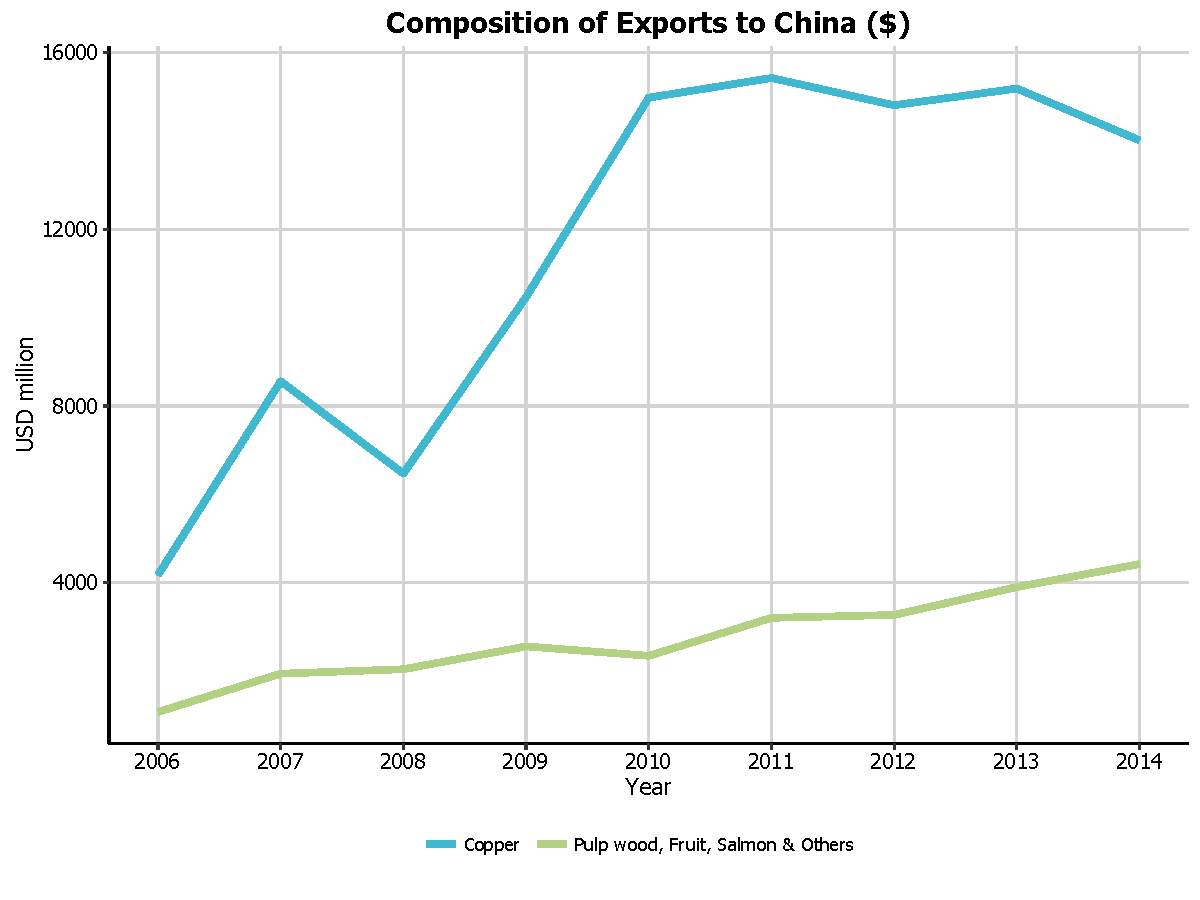
\includegraphics[width=0.55\linewidth]{figures/line_final-1} \end{center}

We will use an international trade \href{http://pachamaltese.github.io/stats/trade-chile-china/copper-data-for-tutorial.csv}{dataset} made by ourselves from different sources (Chile Customs,
Central Bank of Chile and General Directorate of International Economic Relations).

The first thing to do is load in the data and libraries, as below:

\begin{Shaded}
\begin{Highlighting}[]
\KeywordTok{library}\NormalTok{(ggplot2)}
\KeywordTok{library}\NormalTok{(ggthemes)}
\KeywordTok{library}\NormalTok{(extrafont)}

\NormalTok{charts.data <-}\StringTok{ }\KeywordTok{read.csv}\NormalTok{(}\StringTok{"copper-data-for-tutorial.csv"}\NormalTok{)}
\end{Highlighting}
\end{Shaded}

\section{Basic graph}\label{basic-graph}

In order to initialise a plot we tell ggplot that \texttt{charts.data}
is our data, and specify the variables on each axis. We then instruct
ggplot to render this as a line plot by adding the \texttt{geom\_line}
command.

\begin{Shaded}
\begin{Highlighting}[]
\NormalTok{p1 <-}\StringTok{ }\KeywordTok{ggplot}\NormalTok{() +}\StringTok{ }\KeywordTok{geom_line}\NormalTok{(}\KeywordTok{aes}\NormalTok{(}\DataTypeTok{y =} \NormalTok{export, }\DataTypeTok{x =} \NormalTok{year, }\DataTypeTok{colour =} \NormalTok{product), }
\StringTok{\StringTok{        }}\DataTypeTok{data =} \NormalTok{charts.data, }\DataTypeTok{stat=}\StringTok{"identity"}\NormalTok{)}
\NormalTok{p1}
\end{Highlighting}
\end{Shaded}

\begin{center}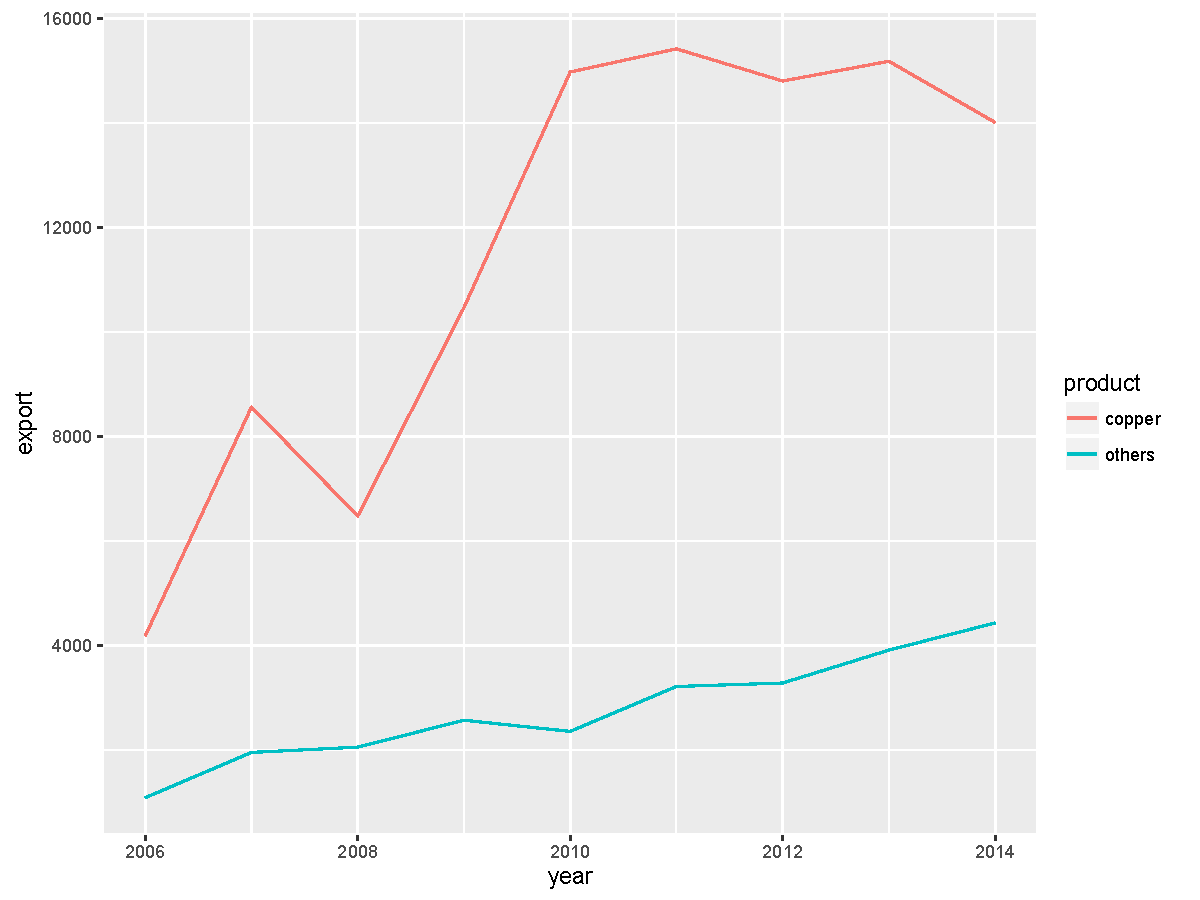
\includegraphics[width=0.55\linewidth]{figures/line_1-1} \end{center}

\section{Adjusting line width}\label{adjusting-line-width}

To change the line width, we add a \texttt{size} argument to
\texttt{geom\_line}.

\begin{Shaded}
\begin{Highlighting}[]
\NormalTok{p1 <-}\StringTok{ }\KeywordTok{ggplot}\NormalTok{() +}\StringTok{ }\KeywordTok{geom_line}\NormalTok{(}\KeywordTok{aes}\NormalTok{(}\DataTypeTok{y =} \NormalTok{export, }\DataTypeTok{x =} \NormalTok{year, }\DataTypeTok{colour =} \NormalTok{product), }
\StringTok{\StringTok{        }}\DataTypeTok{size=}\FloatTok{1.5}\NormalTok{, }\DataTypeTok{data =} \NormalTok{charts.data, }\DataTypeTok{stat=}\StringTok{"identity"}\NormalTok{)}
\NormalTok{p1}
\end{Highlighting}
\end{Shaded}

\begin{center}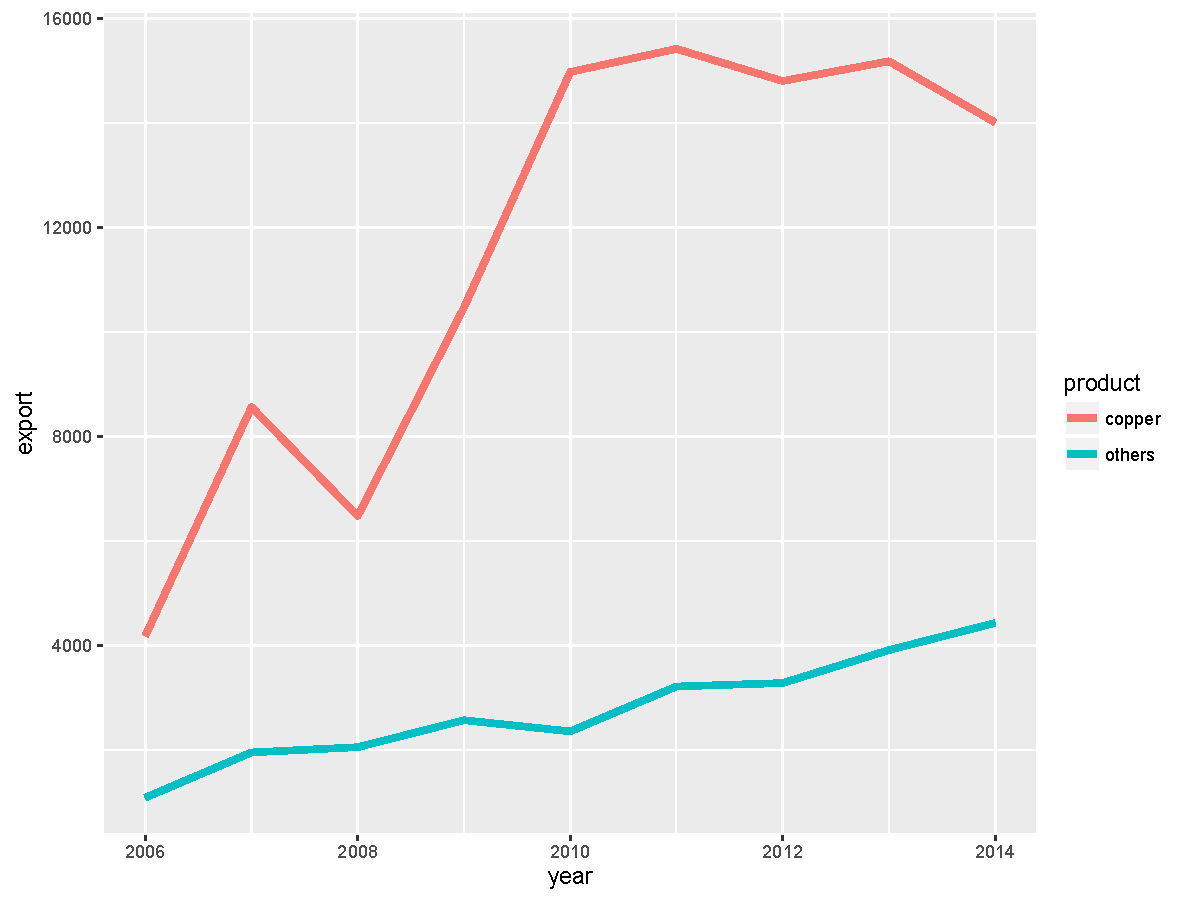
\includegraphics[width=0.55\linewidth]{figures/line_2-1} \end{center}

\section{Changing variables
display}\label{changing-variables-display}

To change the variables displayed name, we need to re-factor our data
labels in \texttt{charts.data} data frame. Then we move the legend to
the bottom using the \texttt{theme} command.

\begin{Shaded}
\begin{Highlighting}[]
\NormalTok{charts.data <-}\StringTok{ }\KeywordTok{as.data.frame}\NormalTok{(charts.data)}
\NormalTok{charts.data$product <-}\StringTok{ }\KeywordTok{factor}\NormalTok{(charts.data$product, }
\StringTok{\StringTok{        }}\DataTypeTok{levels =} \KeywordTok{c}\NormalTok{(}\StringTok{"copper"}\NormalTok{,}\StringTok{"others"}\NormalTok{), }
\StringTok{\StringTok{        }}\DataTypeTok{labels =} \KeywordTok{c}\NormalTok{(}\StringTok{"Copper"}\NormalTok{,}\StringTok{"Pulp wood, Fruit, Salmon & Others"}\NormalTok{))}

\NormalTok{p1 <-}\StringTok{ }\KeywordTok{ggplot}\NormalTok{() +}\StringTok{ }
\StringTok{      }\KeywordTok{geom_line}\NormalTok{(}\KeywordTok{aes}\NormalTok{(}\DataTypeTok{y =} \NormalTok{export, }\DataTypeTok{x =} \NormalTok{year, }\DataTypeTok{colour =} \NormalTok{product), }\DataTypeTok{size=}\FloatTok{1.5}\NormalTok{, }
\StringTok{\StringTok{        }}\DataTypeTok{data =} \NormalTok{charts.data, }\DataTypeTok{stat=}\StringTok{"identity"}\NormalTok{) +}
\StringTok{      }\KeywordTok{theme}\NormalTok{(}\DataTypeTok{legend.position=}\StringTok{"bottom"}\NormalTok{, }\DataTypeTok{legend.direction=}\StringTok{"horizontal"}\NormalTok{, }
\StringTok{\StringTok{        }}\DataTypeTok{legend.title =} \KeywordTok{element_blank}\NormalTok{())}
\NormalTok{p1}
\end{Highlighting}
\end{Shaded}

\begin{center}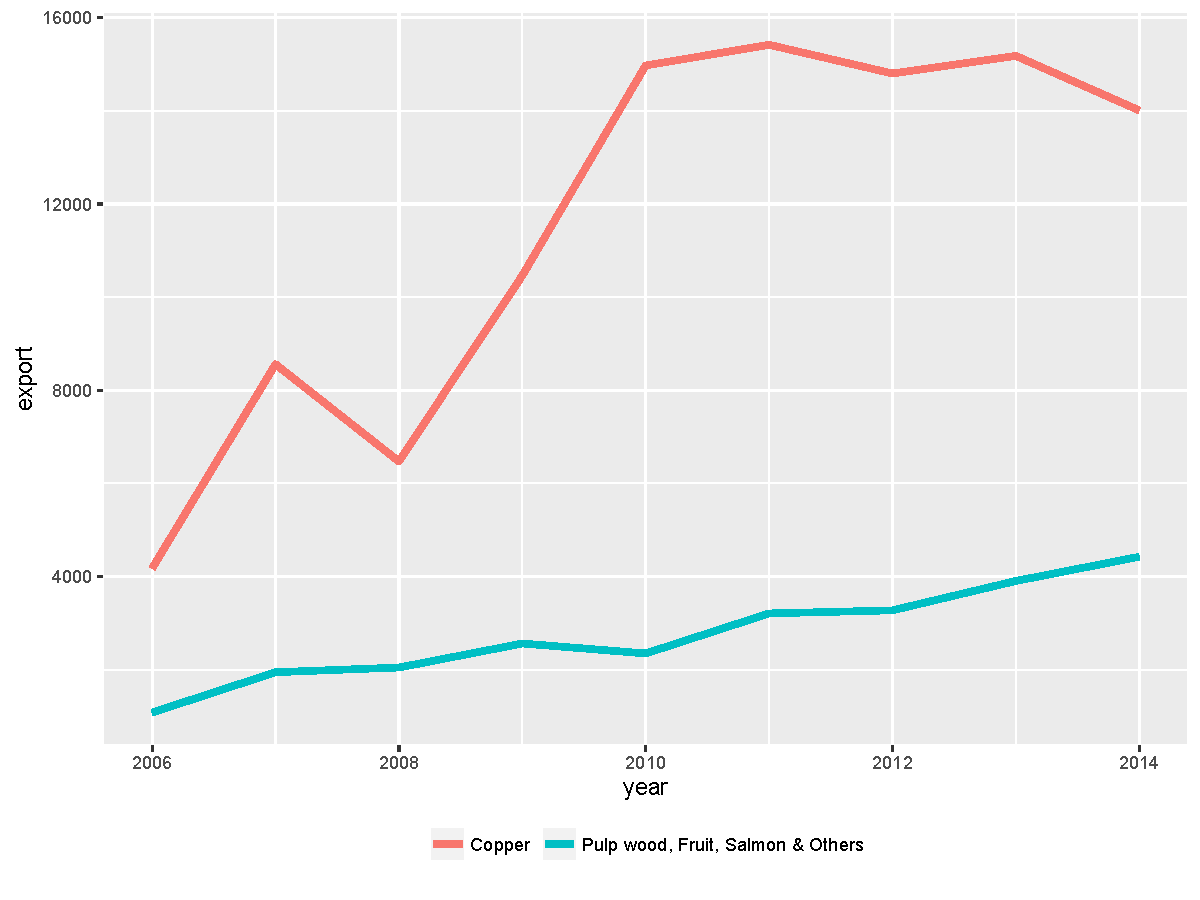
\includegraphics[width=0.55\linewidth]{figures/line_3-1} \end{center}

\section{Adjusting x-axis scale}\label{adjusting-x-axis-scale}

To change the axis tick marks, we use the \texttt{scale\_x\_continuous}
and/or \texttt{scale\_y\_continuous} commands.

\begin{Shaded}
\begin{Highlighting}[]
\NormalTok{p1 <-}\StringTok{ }\NormalTok{p1 +}\StringTok{ }\KeywordTok{scale_x_continuous}\NormalTok{(}\DataTypeTok{breaks=}\KeywordTok{seq}\NormalTok{(}\DecValTok{2006}\NormalTok{,}\DecValTok{2014}\NormalTok{,}\DecValTok{1}\NormalTok{))}
\NormalTok{p1}
\end{Highlighting}
\end{Shaded}

\begin{center}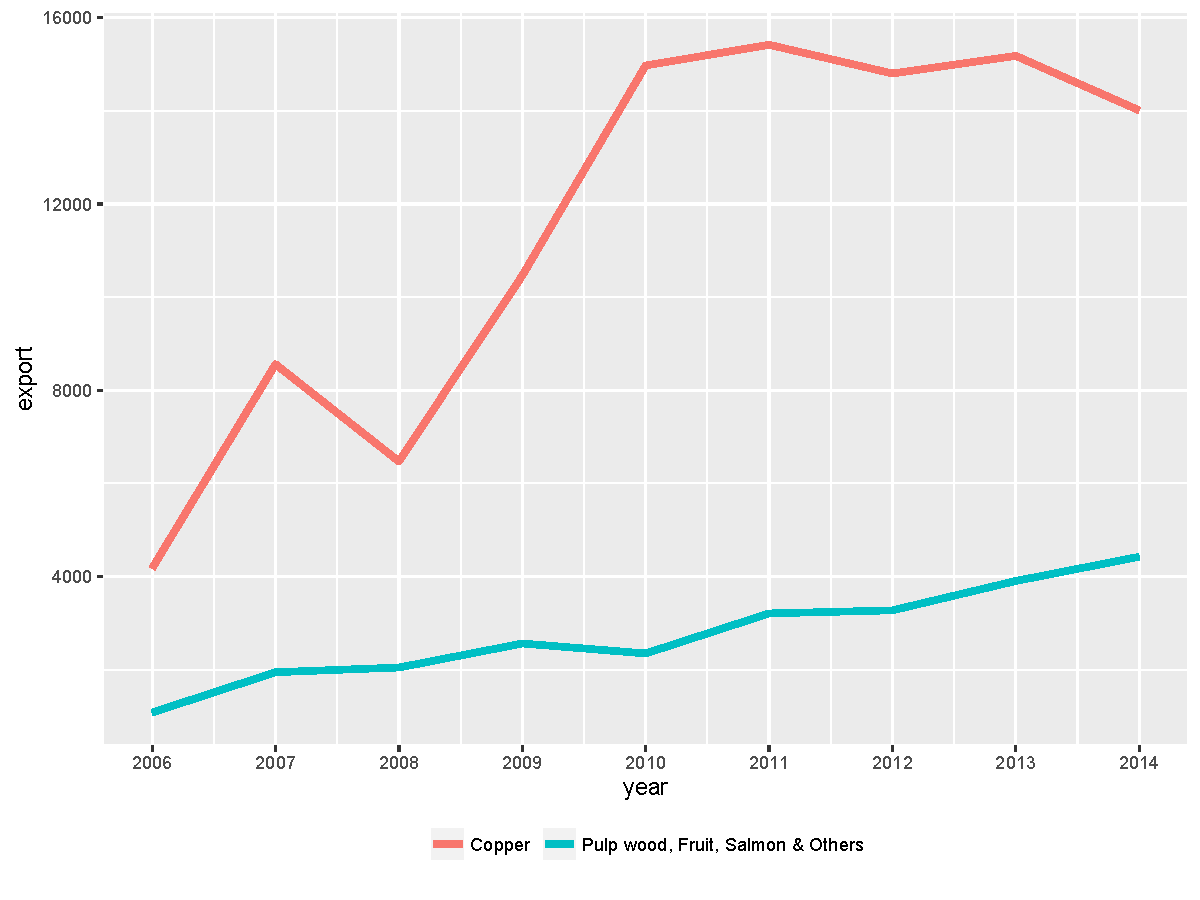
\includegraphics[width=0.55\linewidth]{figures/line_4-1} \end{center}

\section{Adjusting axis labels \& adding
title}\label{adjusting-axis-labels-adding-title}

To add a title, we include the option \texttt{ggtitle} and include the
name of the graph as a string argument, and to change the axis names we
use the \texttt{labs} command.

\begin{Shaded}
\begin{Highlighting}[]
\NormalTok{p1 <-}\StringTok{ }\NormalTok{p1 +}\StringTok{ }\KeywordTok{ggtitle}\NormalTok{(}\StringTok{"Composition of Exports to China ($)"}\NormalTok{) +}
\StringTok{      }\KeywordTok{labs}\NormalTok{(}\DataTypeTok{x=}\StringTok{"Year"}\NormalTok{, }\DataTypeTok{y=}\StringTok{"USD million"}\NormalTok{) }
\NormalTok{p1}
\end{Highlighting}
\end{Shaded}

\begin{center}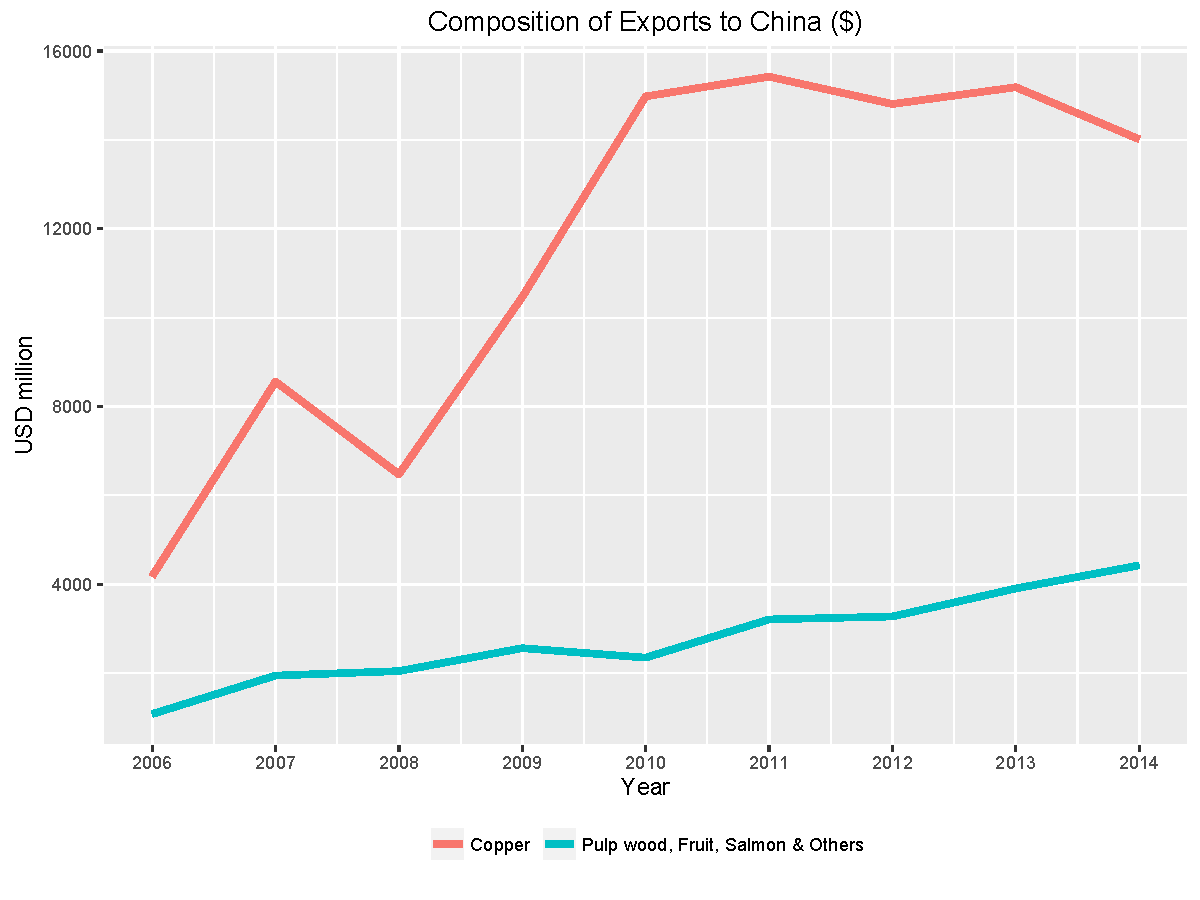
\includegraphics[width=0.55\linewidth]{figures/line_5-1} \end{center}

\section{Adjusting color palette}\label{adjusting-color-palette}

To change the colours, we use the \texttt{scale\_colour\_manual}
command.

\begin{Shaded}
\begin{Highlighting}[]
\NormalTok{colour <-}\StringTok{ }\KeywordTok{c}\NormalTok{(}\StringTok{"#5F9EA0"}\NormalTok{, }\StringTok{"#E1B378"}\NormalTok{)}
\NormalTok{p1 <-}\StringTok{ }\NormalTok{p1 +}\StringTok{ }\KeywordTok{scale_colour_manual}\NormalTok{(}\DataTypeTok{values=}\NormalTok{colour)}
\NormalTok{p1}
\end{Highlighting}
\end{Shaded}

\begin{center}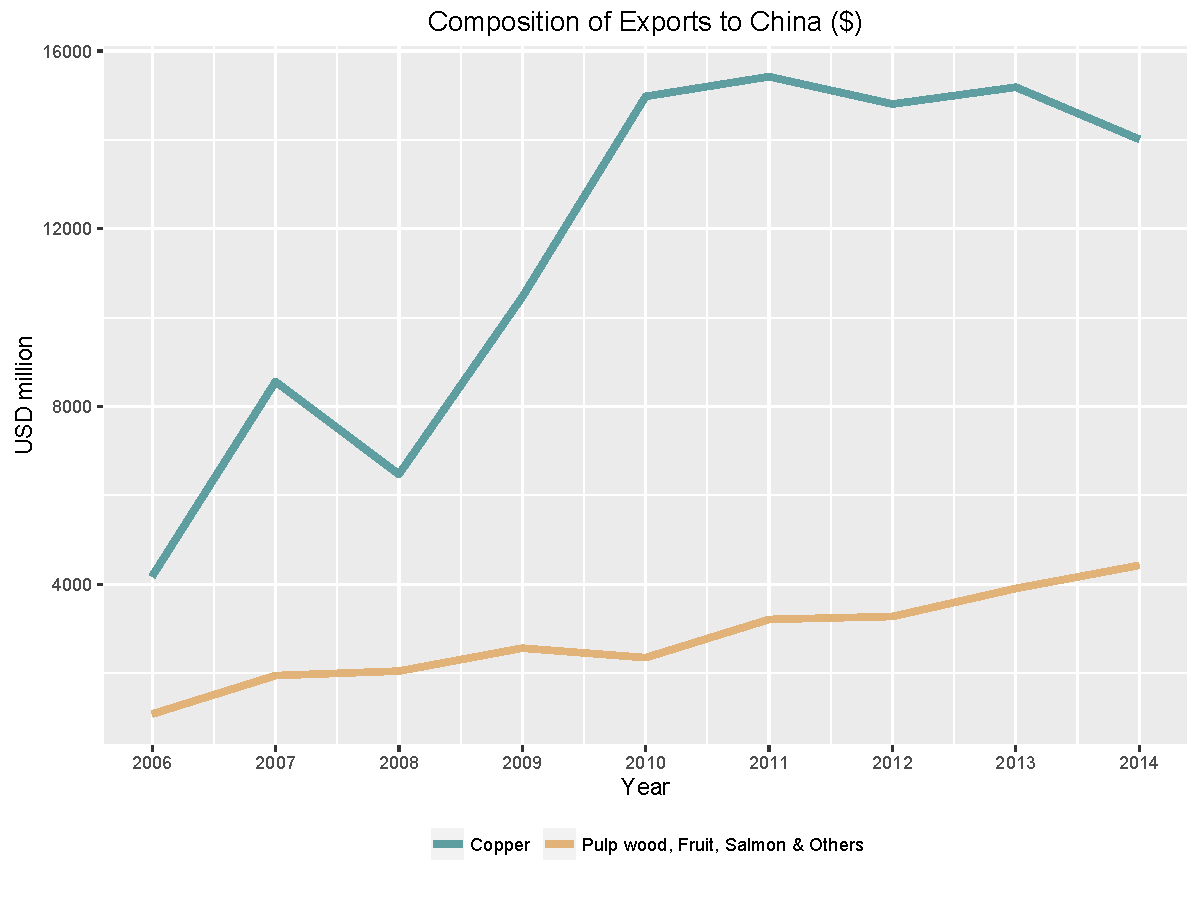
\includegraphics[width=0.55\linewidth]{figures/line_6-1} \end{center}

\section{Using the white theme}\label{using-the-white-theme}

We'll start using a simple theme customisation made adding
\texttt{theme\_bw()} after \texttt{ggplot()}. That theme argument can be
modified to use different themes.

\begin{Shaded}
\begin{Highlighting}[]
\NormalTok{p1 <-}\StringTok{ }\KeywordTok{ggplot}\NormalTok{() +}
\StringTok{      }\KeywordTok{geom_line}\NormalTok{(}\KeywordTok{aes}\NormalTok{(}\DataTypeTok{y =} \NormalTok{export, }\DataTypeTok{x =} \NormalTok{year, }\DataTypeTok{colour =} \NormalTok{product), }\DataTypeTok{size=}\FloatTok{1.5}\NormalTok{, }
\StringTok{\StringTok{        }}\DataTypeTok{data =} \NormalTok{charts.data, }\DataTypeTok{stat=}\StringTok{"identity"}\NormalTok{) +}\StringTok{ }
\StringTok{      }\KeywordTok{scale_x_continuous}\NormalTok{(}\DataTypeTok{breaks=}\KeywordTok{seq}\NormalTok{(}\DecValTok{2006}\NormalTok{,}\DecValTok{2014}\NormalTok{,}\DecValTok{1}\NormalTok{)) +}\StringTok{ }
\StringTok{      }\KeywordTok{labs}\NormalTok{(}\DataTypeTok{x=}\StringTok{"Year"}\NormalTok{, }\DataTypeTok{y=}\StringTok{"USD million"}\NormalTok{) +}\StringTok{ }
\StringTok{      }\KeywordTok{ggtitle}\NormalTok{(}\StringTok{"Composition of Exports to China ($)"}\NormalTok{) +}\StringTok{ }
\StringTok{      }\KeywordTok{scale_colour_manual}\NormalTok{(}\DataTypeTok{values=}\NormalTok{colour) +}
\StringTok{      }\KeywordTok{theme_bw}\NormalTok{() +}
\StringTok{      }\KeywordTok{theme}\NormalTok{(}\DataTypeTok{legend.position=}\StringTok{"bottom"}\NormalTok{, }
\StringTok{        }\DataTypeTok{legend.direction=}\StringTok{"horizontal"}\NormalTok{, }
\StringTok{        }\DataTypeTok{legend.title =} \KeywordTok{element_blank}\NormalTok{()) }
\NormalTok{p1}
\end{Highlighting}
\end{Shaded}

\begin{center}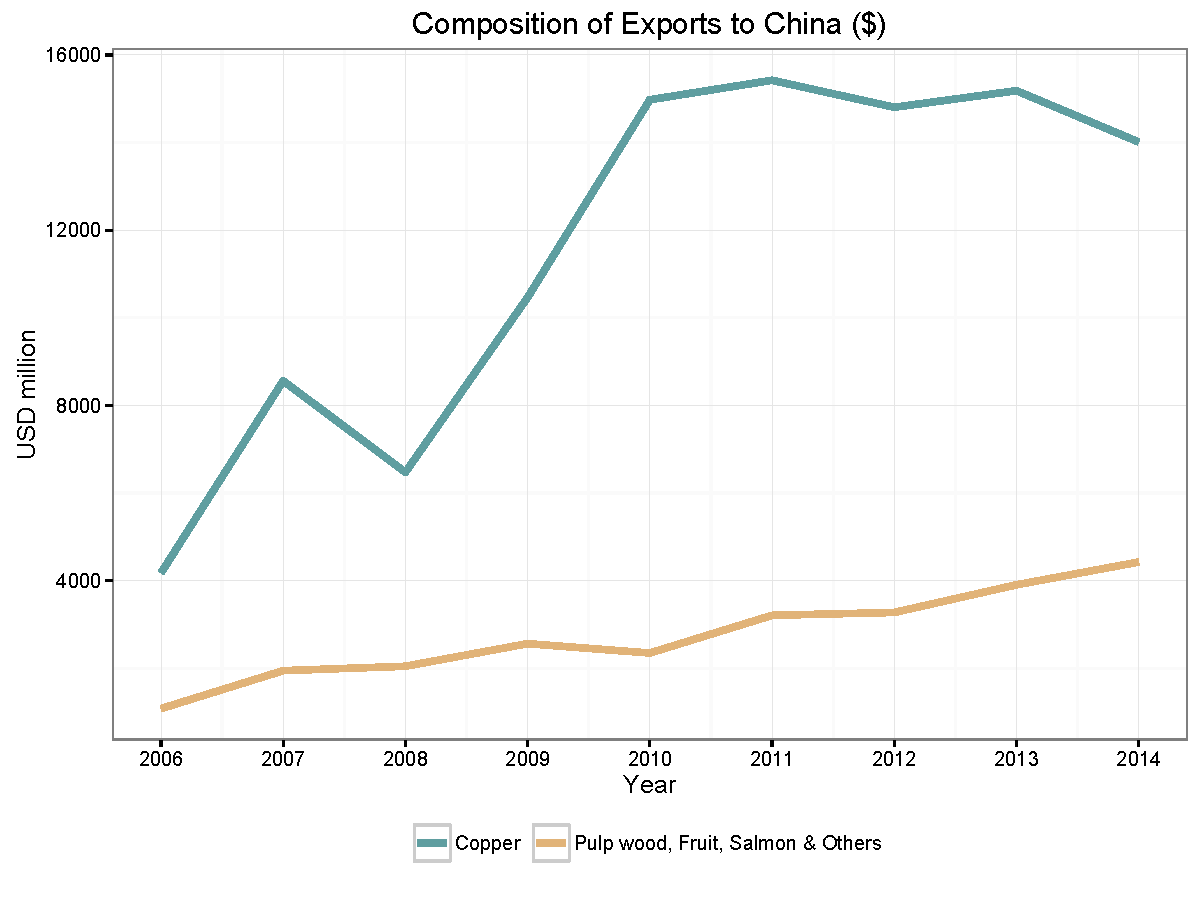
\includegraphics[width=0.55\linewidth]{figures/line_7-1} \end{center}

\section{Creating an XKCD style
chart}\label{creating-an-xkcd-style-chart}

Of course, you may want to create your own themes as well.
\texttt{ggplot2} allows for a very high degree of customisation,
including allowing you to use imported fonts. Below is an example of a
theme Mauricio was able to create which mimics the visual style of
\href{http://xkcd.com/}{XKCD}. In order to create this chart, you first
need to import the XKCD font, install it on your machine and load it
into R using the \texttt{extrafont} package. These instructions are
taken from
\href{https://www.google.com.au/url?sa=t\&rct=j\&q=\&esrc=s\&source=web\&cd=1\&ved=0ahUKEwiWzafchdPJAhVBpJQKHe_LDT8QFggbMAA\&url=https\%3A\%2F\%2Fcran.r-project.org\%2Fweb\%2Fpackages\%2Fxkcd\%2Fvignettes\%2Fxkcd-intro.pdf\&usg=AFQjCNE-KciGY14e-Q1buYIVmTFC0ht__Q\&sig2=DZUwkvIHwfNWtTtkcz94jg}{here}:

\begin{Shaded}
\begin{Highlighting}[]
\KeywordTok{library}\NormalTok{(extrafont)}

\KeywordTok{download.file}\NormalTok{(}\StringTok{"http://simonsoftware.se/other/xkcd.ttf"}\NormalTok{, }
\StringTok{      }\DataTypeTok{dest=}\StringTok{"xkcd.ttf"}\NormalTok{, }\DataTypeTok{mode=}\StringTok{"wb"}\NormalTok{)}
\KeywordTok{system}\NormalTok{(}\StringTok{"mkdir ~/.fonts"}\NormalTok{)}
\KeywordTok{system}\NormalTok{(}\StringTok{"cp xkcd.ttf  ~/.fonts"}\NormalTok{)}
\KeywordTok{font_import}\NormalTok{(}\DataTypeTok{paths =} \StringTok{"~/.fonts"}\NormalTok{, }\DataTypeTok{pattern=}\StringTok{"[X/x]kcd"}\NormalTok{)}
\KeywordTok{fonts}\NormalTok{()}
\KeywordTok{loadfonts}\NormalTok{()}
\end{Highlighting}
\end{Shaded}

You can then create your graph:

\begin{Shaded}
\begin{Highlighting}[]
\NormalTok{fill <-}\StringTok{ }\KeywordTok{c}\NormalTok{(}\StringTok{"#56B4E9"}\NormalTok{, }\StringTok{"#ff69b4"}\NormalTok{)}

\NormalTok{p1 <-}\StringTok{ }\KeywordTok{ggplot}\NormalTok{() +}\StringTok{ }
\StringTok{      }\KeywordTok{geom_line}\NormalTok{(}\KeywordTok{aes}\NormalTok{(}\DataTypeTok{y =} \NormalTok{export, }\DataTypeTok{x =} \NormalTok{year, }\DataTypeTok{colour =} \NormalTok{product), }\DataTypeTok{size=}\FloatTok{1.5}\NormalTok{, }
\StringTok{        }\DataTypeTok{data =} \NormalTok{charts.data, }\DataTypeTok{stat=}\StringTok{"identity"}\NormalTok{) +}\StringTok{ }
\StringTok{      }\KeywordTok{scale_x_continuous}\NormalTok{(}\DataTypeTok{breaks=}\KeywordTok{seq}\NormalTok{(}\DecValTok{2006}\NormalTok{,}\DecValTok{2014}\NormalTok{,}\DecValTok{1}\NormalTok{)) +}\StringTok{ }
\StringTok{      }\KeywordTok{labs}\NormalTok{(}\DataTypeTok{x=}\StringTok{"Year"}\NormalTok{, }\DataTypeTok{y=}\StringTok{"USD million"}\NormalTok{) +}\StringTok{ }
\StringTok{      }\KeywordTok{ggtitle}\NormalTok{(}\StringTok{"Composition of Exports to China ($)"}\NormalTok{) +}\StringTok{ }
\StringTok{      }\KeywordTok{scale_color_manual}\NormalTok{(}\DataTypeTok{values=}\NormalTok{fill) +}\StringTok{ }
\StringTok{      }\KeywordTok{theme}\NormalTok{(}\DataTypeTok{axis.text.x=}\KeywordTok{element_text}\NormalTok{(}\DataTypeTok{colour=}\StringTok{"black"}\NormalTok{, }\DataTypeTok{size =} \DecValTok{10}\NormalTok{), }
\StringTok{        }\DataTypeTok{axis.text.y=}\KeywordTok{element_text}\NormalTok{(}\DataTypeTok{colour=}\StringTok{"black"}\NormalTok{, }\DataTypeTok{size =} \DecValTok{10}\NormalTok{),}
\StringTok{        }\DataTypeTok{axis.line.x =} \KeywordTok{element_line}\NormalTok{(}\DataTypeTok{size=}\NormalTok{.}\DecValTok{5}\NormalTok{, }\DataTypeTok{colour =} \StringTok{"black"}\NormalTok{),}
\StringTok{        }\DataTypeTok{axis.line.y =} \KeywordTok{element_line}\NormalTok{(}\DataTypeTok{size=}\NormalTok{.}\DecValTok{5}\NormalTok{, }\DataTypeTok{colour =} \StringTok{"black"}\NormalTok{),}
\StringTok{        }\DataTypeTok{legend.key=}\KeywordTok{element_rect}\NormalTok{(}\DataTypeTok{fill=}\StringTok{"white"}\NormalTok{, }\DataTypeTok{colour=}\StringTok{"white"}\NormalTok{),}
\StringTok{        }\DataTypeTok{legend.position=}\StringTok{"bottom"}\NormalTok{, }\DataTypeTok{legend.direction=}\StringTok{"horizontal"}\NormalTok{, }
\StringTok{        }\DataTypeTok{legend.title =} \KeywordTok{element_blank}\NormalTok{(),}
\StringTok{        }\DataTypeTok{panel.grid.major =} \KeywordTok{element_blank}\NormalTok{(),}
\StringTok{        }\DataTypeTok{panel.grid.minor =} \KeywordTok{element_blank}\NormalTok{(), }\DataTypeTok{panel.border =} \KeywordTok{element_blank}\NormalTok{(), }
\StringTok{        }\DataTypeTok{panel.background =} \KeywordTok{element_blank}\NormalTok{(),}
\StringTok{        }\DataTypeTok{plot.title=}\KeywordTok{element_text}\NormalTok{(}\DataTypeTok{family=}\StringTok{"xkcd-Regular"}\NormalTok{), }
\StringTok{        }\DataTypeTok{text=}\KeywordTok{element_text}\NormalTok{(}\DataTypeTok{family=}\StringTok{"xkcd-Regular"}\NormalTok{)) }
\NormalTok{p1}
\end{Highlighting}
\end{Shaded}

\begin{center}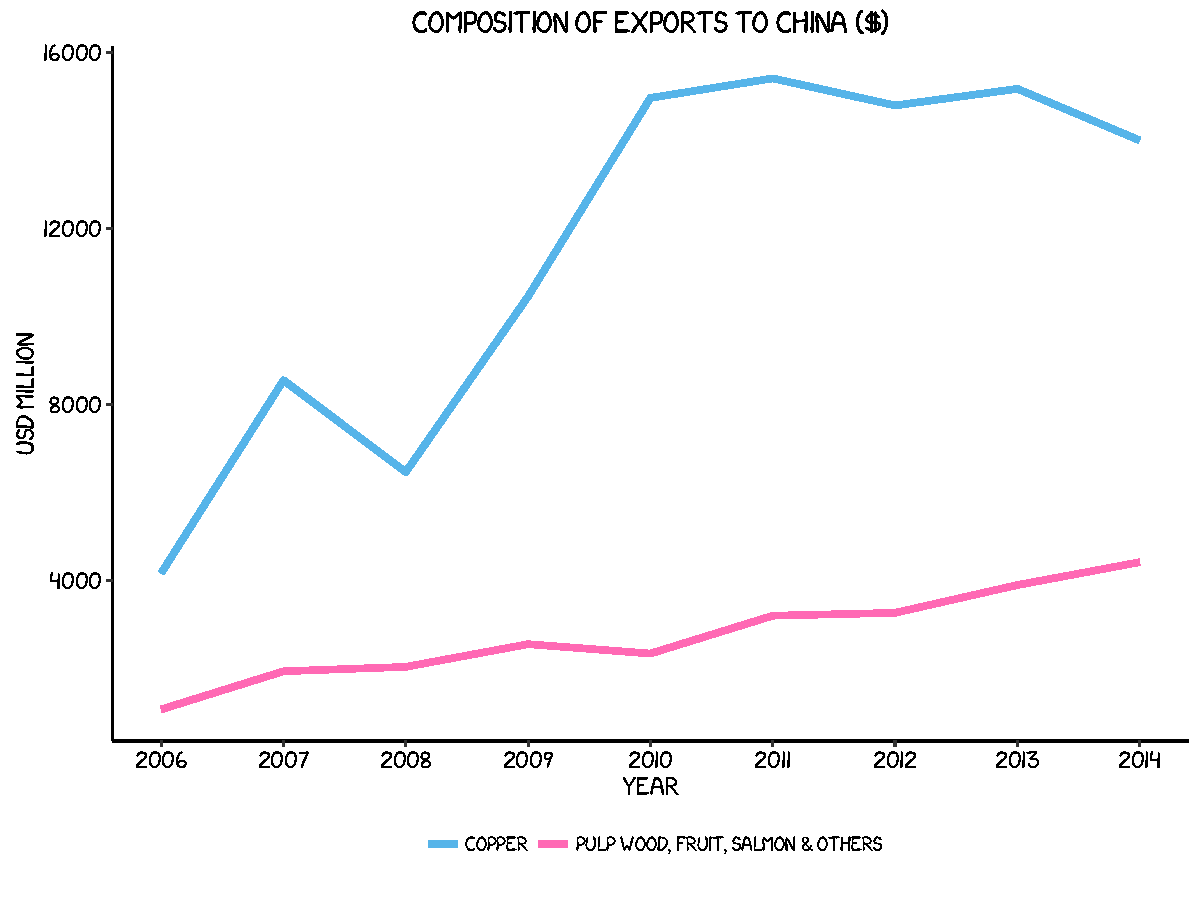
\includegraphics[width=0.55\linewidth]{figures/line_8-1} \end{center}

\section{\texorpdfstring{Using `The Economist'
theme}{Using The Economist theme}}\label{using-the-economist-theme}

There are a wider range of pre-built themes available as part of the
\texttt{ggthemes} package (more information on these
\href{https://cran.r-project.org/web/packages/ggthemes/vignettes/ggthemes.html}{here}).
Below we've applied \texttt{theme\_economist()}, which approximates
graphs in the Economist magazine. It is also important that the font
change argument inside \texttt{theme} is optional and it's only to
obtain a more similar result compared to the original. For an exact
result you need `Officina Sans' which is a commercial font and is
available \href{http://www.myfonts.com/fonts/itc/officina-sans/}{here}.

\begin{Shaded}
\begin{Highlighting}[]
\NormalTok{p1 <-}\StringTok{ }\KeywordTok{ggplot}\NormalTok{() +}
\StringTok{      }\KeywordTok{geom_line}\NormalTok{(}\KeywordTok{aes}\NormalTok{(}\DataTypeTok{y =} \NormalTok{export, }\DataTypeTok{x =} \NormalTok{year, }\DataTypeTok{colour =} \NormalTok{product), }\DataTypeTok{size=}\FloatTok{1.5}\NormalTok{, }
\StringTok{        }\DataTypeTok{data =} \NormalTok{charts.data, }\DataTypeTok{stat=}\StringTok{"identity"}\NormalTok{) +}\StringTok{ }
\StringTok{      }\KeywordTok{scale_x_continuous}\NormalTok{(}\DataTypeTok{breaks=}\KeywordTok{seq}\NormalTok{(}\DecValTok{2006}\NormalTok{,}\DecValTok{2014}\NormalTok{,}\DecValTok{1}\NormalTok{)) +}\StringTok{ }
\StringTok{      }\KeywordTok{labs}\NormalTok{(}\DataTypeTok{x=}\StringTok{"Year"}\NormalTok{, }\DataTypeTok{y=}\StringTok{"USD million"}\NormalTok{) +}\StringTok{ }
\StringTok{      }\KeywordTok{ggtitle}\NormalTok{(}\StringTok{"Composition of Exports to China ($)"}\NormalTok{) +}
\StringTok{      }\KeywordTok{theme_economist}\NormalTok{() +}\StringTok{ }\KeywordTok{scale_colour_economist}\NormalTok{() +}
\StringTok{      }\KeywordTok{theme}\NormalTok{(}\DataTypeTok{axis.line.x =} \KeywordTok{element_line}\NormalTok{(}\DataTypeTok{size=}\NormalTok{.}\DecValTok{5}\NormalTok{, }\DataTypeTok{colour =} \StringTok{"black"}\NormalTok{), }
\StringTok{        }\DataTypeTok{axis.line.y =} \KeywordTok{element_line}\NormalTok{(}\DataTypeTok{size=}\NormalTok{.}\DecValTok{5}\NormalTok{, }\DataTypeTok{colour =} \StringTok{"black"}\NormalTok{),}
\StringTok{        }\DataTypeTok{legend.position=}\StringTok{"bottom"}\NormalTok{, }
\StringTok{        }\DataTypeTok{legend.direction=}\StringTok{"horizontal"}\NormalTok{, }
\StringTok{        }\DataTypeTok{legend.title =} \KeywordTok{element_blank}\NormalTok{(),}
\StringTok{        }\DataTypeTok{plot.title=}\KeywordTok{element_text}\NormalTok{(}\DataTypeTok{family=}\StringTok{"OfficinaSanITC-Book"}\NormalTok{),}
\StringTok{        }\DataTypeTok{text=}\KeywordTok{element_text}\NormalTok{(}\DataTypeTok{family=}\StringTok{"OfficinaSanITC-Book"}\NormalTok{)) }
\NormalTok{p1}
\end{Highlighting}
\end{Shaded}

\begin{center}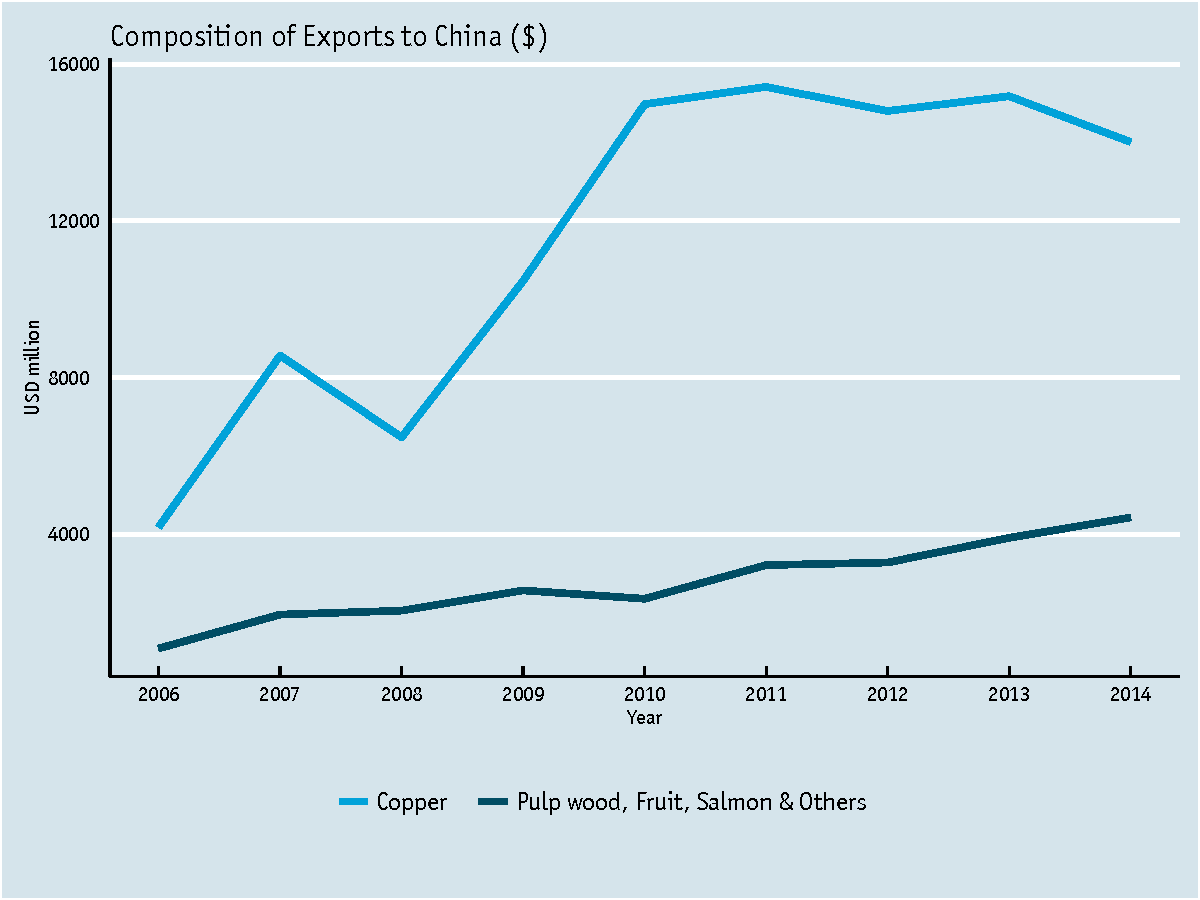
\includegraphics[width=0.55\linewidth]{figures/line_9-1} \end{center}

\section{Creating your own theme}\label{creating-your-own-theme}

As before, you can modify your plots a lot as \texttt{ggplot2} allows
many customisations. Here we present our original result shown at the
top of page.

\begin{Shaded}
\begin{Highlighting}[]
\NormalTok{colour <-}\StringTok{ }\KeywordTok{c}\NormalTok{(}\StringTok{"#40b8d0"}\NormalTok{, }\StringTok{"#b2d183"}\NormalTok{)}

\NormalTok{p1 <-}\StringTok{ }\KeywordTok{ggplot}\NormalTok{() +}\StringTok{ }
\StringTok{      }\KeywordTok{geom_line}\NormalTok{(}\KeywordTok{aes}\NormalTok{(}\DataTypeTok{y =} \NormalTok{export, }\DataTypeTok{x =} \NormalTok{year, }\DataTypeTok{colour =} \NormalTok{product), }\DataTypeTok{size=}\FloatTok{1.5}\NormalTok{, }
\StringTok{        }\DataTypeTok{data =} \NormalTok{charts.data, }\DataTypeTok{stat=}\StringTok{"identity"}\NormalTok{) +}\StringTok{ }
\StringTok{      }\KeywordTok{scale_x_continuous}\NormalTok{(}\DataTypeTok{breaks=}\KeywordTok{seq}\NormalTok{(}\DecValTok{2006}\NormalTok{,}\DecValTok{2014}\NormalTok{,}\DecValTok{1}\NormalTok{)) +}\StringTok{ }
\StringTok{      }\KeywordTok{labs}\NormalTok{(}\DataTypeTok{x=}\StringTok{"Year"}\NormalTok{, }\DataTypeTok{y=}\StringTok{"USD million"}\NormalTok{) +}\StringTok{ }
\StringTok{      }\KeywordTok{ggtitle}\NormalTok{(}\StringTok{"Composition of Exports to China ($)"}\NormalTok{) +}\StringTok{ }
\StringTok{      }\KeywordTok{scale_colour_manual}\NormalTok{(}\DataTypeTok{values=}\NormalTok{colour) +}\StringTok{ }
\StringTok{      }\KeywordTok{theme}\NormalTok{(}\DataTypeTok{axis.line.x =} \KeywordTok{element_line}\NormalTok{(}\DataTypeTok{size=}\NormalTok{.}\DecValTok{5}\NormalTok{, }\DataTypeTok{colour =} \StringTok{"black"}\NormalTok{), }
\StringTok{        }\DataTypeTok{axis.line.y =} \KeywordTok{element_line}\NormalTok{(}\DataTypeTok{size=}\NormalTok{.}\DecValTok{5}\NormalTok{, }\DataTypeTok{colour =} \StringTok{"black"}\NormalTok{), }
\StringTok{        }\DataTypeTok{axis.text.x=}\KeywordTok{element_text}\NormalTok{(}\DataTypeTok{colour=}\StringTok{"black"}\NormalTok{, }\DataTypeTok{size =} \DecValTok{10}\NormalTok{), }
\StringTok{        }\DataTypeTok{axis.text.y=}\KeywordTok{element_text}\NormalTok{(}\DataTypeTok{colour=}\StringTok{"black"}\NormalTok{, }\DataTypeTok{size =} \DecValTok{10}\NormalTok{),}
\StringTok{        }\DataTypeTok{legend.key=}\KeywordTok{element_rect}\NormalTok{(}\DataTypeTok{fill=}\StringTok{"white"}\NormalTok{, }\DataTypeTok{colour=}\StringTok{"white"}\NormalTok{),}
\StringTok{        }\DataTypeTok{legend.position=}\StringTok{"bottom"}\NormalTok{, }\DataTypeTok{legend.direction=}\StringTok{"horizontal"}\NormalTok{, }
\StringTok{        }\DataTypeTok{legend.title =} \KeywordTok{element_blank}\NormalTok{(),}
\StringTok{        }\DataTypeTok{panel.grid.major =} \KeywordTok{element_line}\NormalTok{(}\DataTypeTok{colour =} \StringTok{"#d3d3d3"}\NormalTok{), }
\StringTok{        }\DataTypeTok{panel.grid.minor =} \KeywordTok{element_blank}\NormalTok{(), }
\StringTok{        }\DataTypeTok{panel.border =} \KeywordTok{element_blank}\NormalTok{(), }
\StringTok{        }\DataTypeTok{panel.background =} \KeywordTok{element_blank}\NormalTok{(),}
\StringTok{        }\DataTypeTok{plot.title =} \KeywordTok{element_text}\NormalTok{(}\DataTypeTok{size =} \DecValTok{14}\NormalTok{, }\DataTypeTok{family =} \StringTok{"Tahoma"}\NormalTok{, }\DataTypeTok{face =} \StringTok{"bold"}\NormalTok{), }
\StringTok{        }\DataTypeTok{text=}\KeywordTok{element_text}\NormalTok{(}\DataTypeTok{family=}\StringTok{"Tahoma"}\NormalTok{)) }
\NormalTok{p1}
\end{Highlighting}
\end{Shaded}

\begin{center}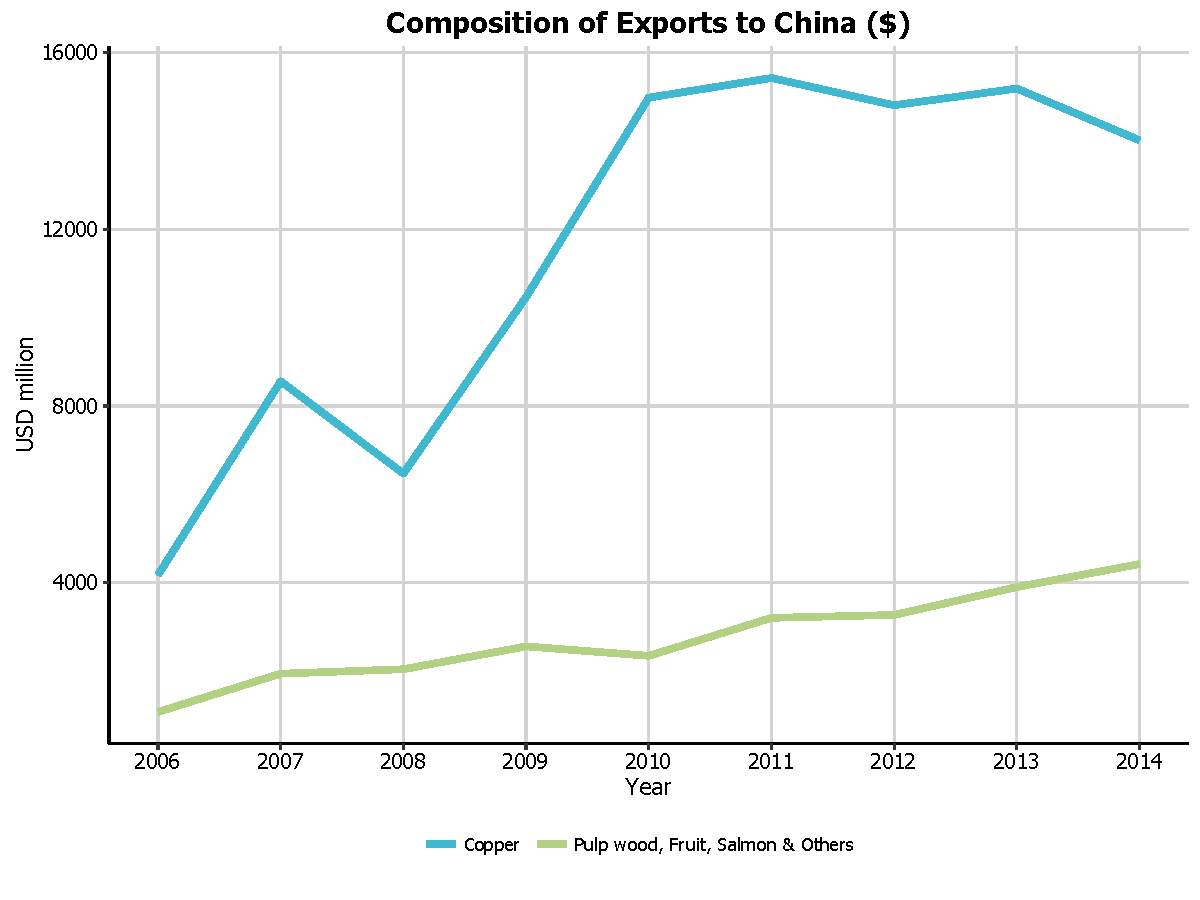
\includegraphics[width=0.55\linewidth]{figures/line_11-1} \end{center}
\chapter{Area Plots}\label{area-plots}

In this part, we will work towards creating the area plot below. We will
take you from a basic area plot and explain all the customisations we
add to the code step-by-step.

\begin{center}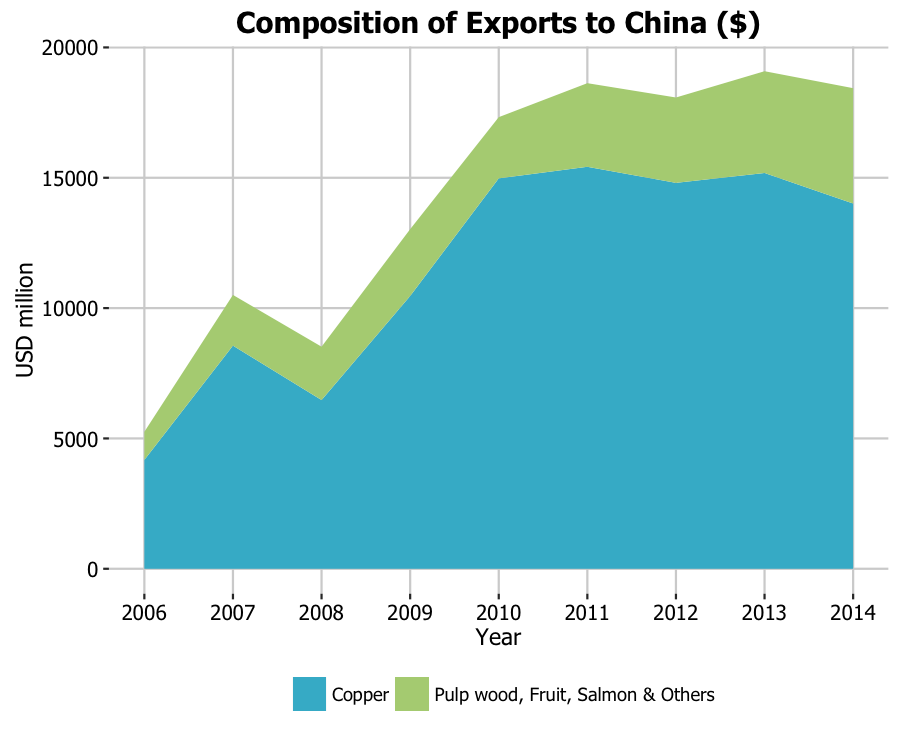
\includegraphics[width=0.55\linewidth]{0_all_posts_pdf/area_final-1} \end{center}

We will use an international trade \href{http://pachamaltese.github.io/stats/trade-chile-china/copper-data-for-tutorial.csv}{dataset} made by ourselves from different sources (Chile Customs,
Central Bank of Chile and General Directorate of International Economic Relations).

\section{Basic graph}\label{basic-graph-1}

The first thing to do is load in the data and libraries, as below:

\begin{Shaded}
\begin{Highlighting}[]
\KeywordTok{library}\NormalTok{(ggplot2)}
\KeywordTok{library}\NormalTok{(ggthemes)}
\KeywordTok{library}\NormalTok{(extrafont)}
\KeywordTok{library}\NormalTok{(plyr)}
\NormalTok{charts.data <-}\StringTok{ }\KeywordTok{read.csv}\NormalTok{(}\StringTok{"copper-data-for-tutorial.csv"}\NormalTok{)}
\end{Highlighting}
\end{Shaded}

In order to initialise a plot we tell ggplot that \texttt{charts.data}
is our data, and specify the variables on each axis. We then instruct
ggplot to render this as an area plot by adding the \texttt{geom\_area}
command.

\begin{Shaded}
\begin{Highlighting}[]
\NormalTok{charts.data <-}\StringTok{ }\KeywordTok{read.csv}\NormalTok{(}\StringTok{"copper-data-for-tutorial.csv"}\NormalTok{)}

\NormalTok{p2 <-}\StringTok{ }\KeywordTok{ggplot}\NormalTok{() +}\StringTok{ }\KeywordTok{geom_area}\NormalTok{(}\KeywordTok{aes}\NormalTok{(}\DataTypeTok{y =} \NormalTok{export, }\DataTypeTok{x =} \NormalTok{year, }\DataTypeTok{fill =} \NormalTok{product), }
\StringTok{        }\DataTypeTok{data =} \NormalTok{charts.data, }\DataTypeTok{stat=}\StringTok{"identity"}\NormalTok{)}
\NormalTok{p2}
\end{Highlighting}
\end{Shaded}

\begin{center}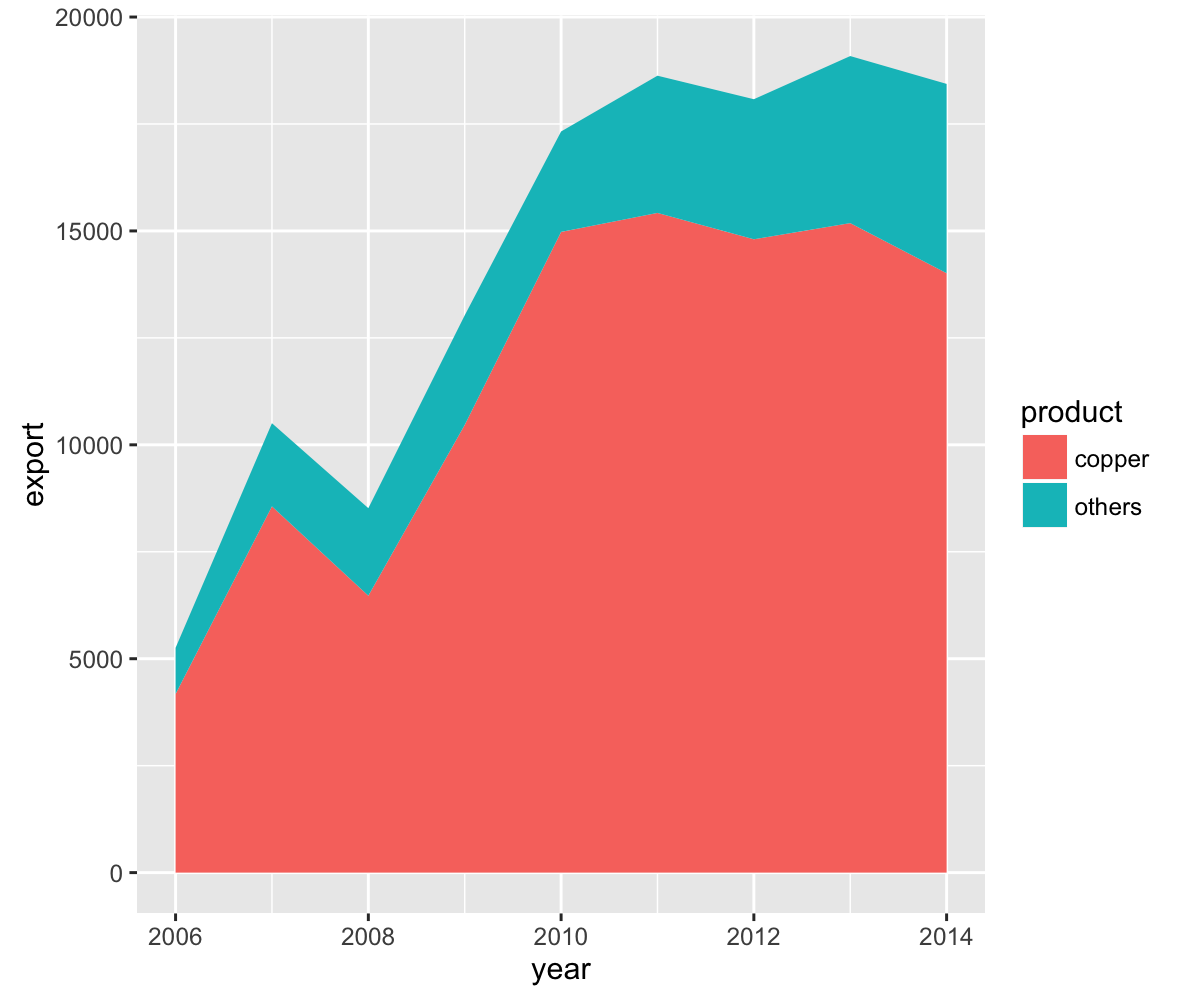
\includegraphics[width=0.55\linewidth]{0_all_posts_pdf/area_1-1} \end{center}

\section{Adjusting legend position}\label{adjusting-legend-position}

To adjust the position of the legend from the default spot of right of
the graph, we add the \texttt{theme} option and specify the
\texttt{legend.position="bottom"} argument. We can also change the title
to blank using the \texttt{legend.title\ =\ element\_blank()} argument
and change the legend shape using the
\texttt{legend.direction="horizontal"} argument.

\begin{Shaded}
\begin{Highlighting}[]
\NormalTok{charts.data <-}\StringTok{ }\KeywordTok{ddply}\NormalTok{(charts.data, .(year), transform, }
\StringTok{        }\DataTypeTok{pos =} \KeywordTok{cumsum}\NormalTok{(export) -}\StringTok{ }\NormalTok{(}\FloatTok{0.5} \NormalTok{*}\StringTok{ }\NormalTok{export))}

\NormalTok{p2 <-}\StringTok{ }\NormalTok{p2 +}\StringTok{ }\KeywordTok{theme}\NormalTok{(}\DataTypeTok{legend.position=}\StringTok{"bottom"}\NormalTok{, }\DataTypeTok{legend.direction=}\StringTok{"horizontal"}\NormalTok{, }
\StringTok{        }\DataTypeTok{legend.title =} \KeywordTok{element_blank}\NormalTok{())}
\NormalTok{p2}
\end{Highlighting}
\end{Shaded}

\begin{center}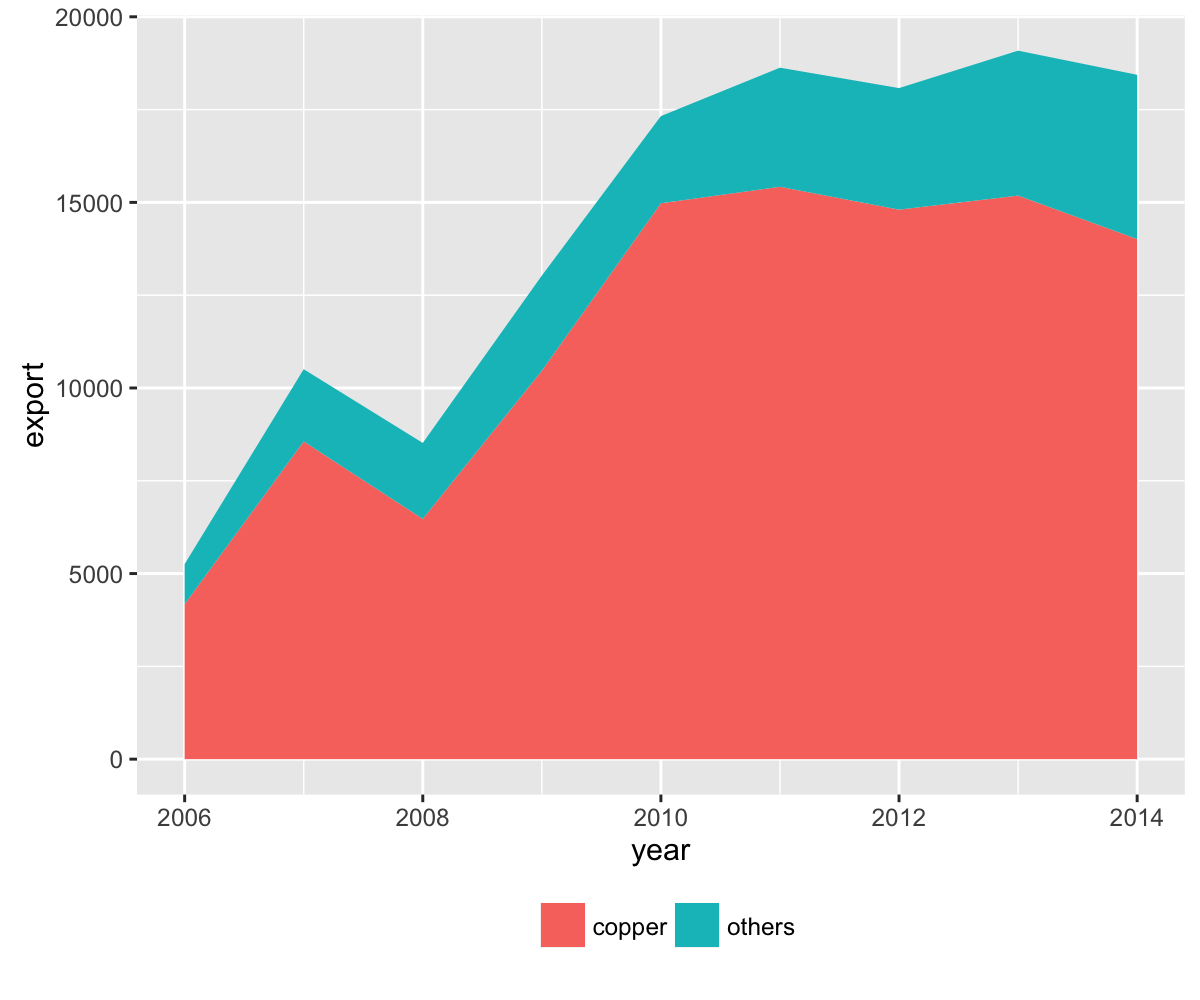
\includegraphics[width=0.55\linewidth]{0_all_posts_pdf/area_2-1} \end{center}

\section{Changing variables
display}\label{changing-variables-display-1}

To change the variables displayed name, we need to re-factor our data
labels in \texttt{charts.data} data frame.

\begin{Shaded}
\begin{Highlighting}[]
\NormalTok{charts.data <-}\StringTok{ }\KeywordTok{as.data.frame}\NormalTok{(charts.data)}
\NormalTok{charts.data$product <-}\StringTok{ }\KeywordTok{factor}\NormalTok{(charts.data$product, }
\StringTok{        }\DataTypeTok{levels =} \KeywordTok{c}\NormalTok{(}\StringTok{"copper"}\NormalTok{,}\StringTok{"others"}\NormalTok{), }
\StringTok{        }\DataTypeTok{labels =} \KeywordTok{c}\NormalTok{(}\StringTok{"Copper"}\NormalTok{,}\StringTok{"Pulp wood, Fruit, Salmon & Others"}\NormalTok{))}

\NormalTok{p2 <-}\StringTok{ }\KeywordTok{ggplot}\NormalTok{() +}\StringTok{ }
\StringTok{      }\KeywordTok{geom_area}\NormalTok{(}\KeywordTok{aes}\NormalTok{(}\DataTypeTok{y =} \NormalTok{export, }\DataTypeTok{x =} \NormalTok{year, }\DataTypeTok{fill =} \NormalTok{product), }\DataTypeTok{data =} \NormalTok{charts.data, }
\StringTok{        }\DataTypeTok{stat=}\StringTok{"identity"}\NormalTok{) +}\StringTok{ }
\StringTok{      }\KeywordTok{theme}\NormalTok{(}\DataTypeTok{legend.position=}\StringTok{"bottom"}\NormalTok{, }\DataTypeTok{legend.direction=}\StringTok{"horizontal"}\NormalTok{, }
\StringTok{        }\DataTypeTok{legend.title =} \KeywordTok{element_blank}\NormalTok{())}
\NormalTok{p2}
\end{Highlighting}
\end{Shaded}

\begin{center}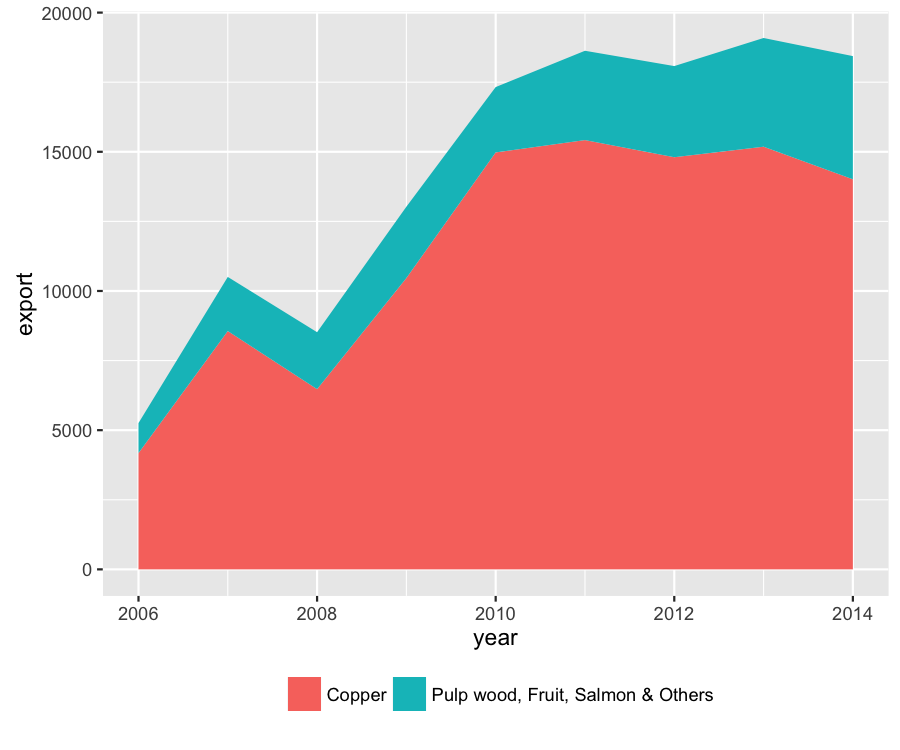
\includegraphics[width=0.55\linewidth]{0_all_posts_pdf/area_3-1} \end{center}

\section{Adjusting x-axis scale}\label{adjusting-x-axis-scale-1}

To change the axis tick marks, we use the \texttt{scale\_x\_continuous}
and/or \texttt{scale\_y\_continuous} commands.

\begin{Shaded}
\begin{Highlighting}[]
\NormalTok{p2 <-}\StringTok{ }\NormalTok{p2 +}\StringTok{ }\KeywordTok{scale_x_continuous}\NormalTok{(}\DataTypeTok{breaks=}\KeywordTok{seq}\NormalTok{(}\DecValTok{2006}\NormalTok{,}\DecValTok{2014}\NormalTok{,}\DecValTok{1}\NormalTok{))}
\NormalTok{p2}
\end{Highlighting}
\end{Shaded}

\begin{center}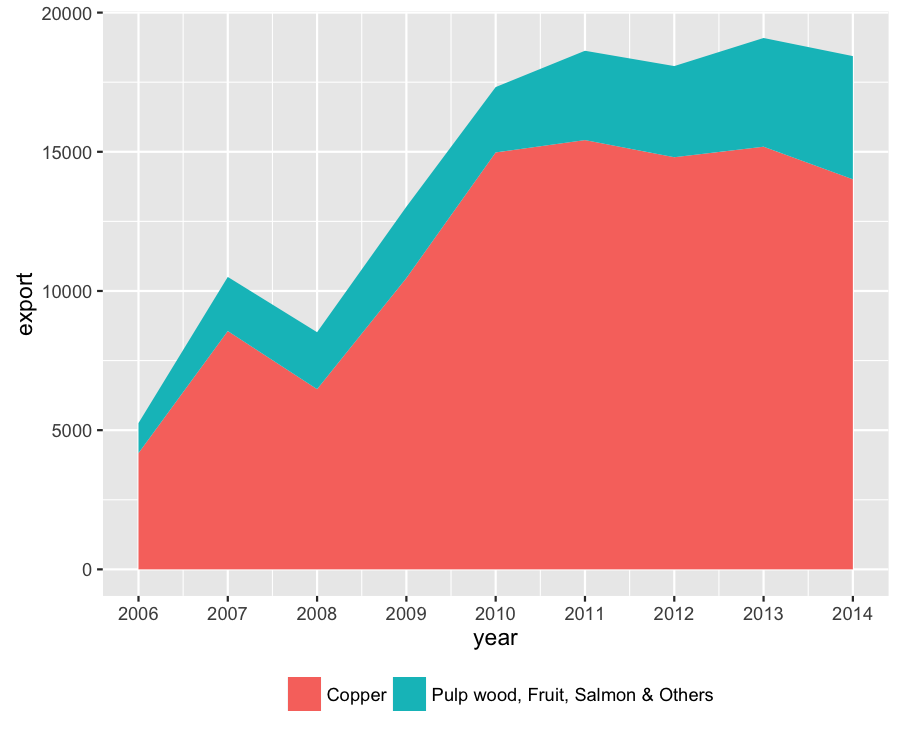
\includegraphics[width=0.55\linewidth]{0_all_posts_pdf/area_4-1} \end{center}

\section{Adjusting axis labels \& adding
title}\label{adjusting-axis-labels-adding-title-1}

To add a title, we include the option \texttt{ggtitle} and include the
name of the graph as a string argument, and to change the axis names we
use the \texttt{labs} command.

\begin{Shaded}
\begin{Highlighting}[]
\NormalTok{p2 <-}\StringTok{ }\NormalTok{p2 +}\StringTok{ }\KeywordTok{ggtitle}\NormalTok{(}\StringTok{"Composition of Exports to China ($)"}\NormalTok{) +}\StringTok{ }
\StringTok{      }\KeywordTok{labs}\NormalTok{(}\DataTypeTok{x=}\StringTok{"Year"}\NormalTok{, }\DataTypeTok{y=}\StringTok{"USD million"}\NormalTok{) }
\NormalTok{p2}
\end{Highlighting}
\end{Shaded}

\begin{center}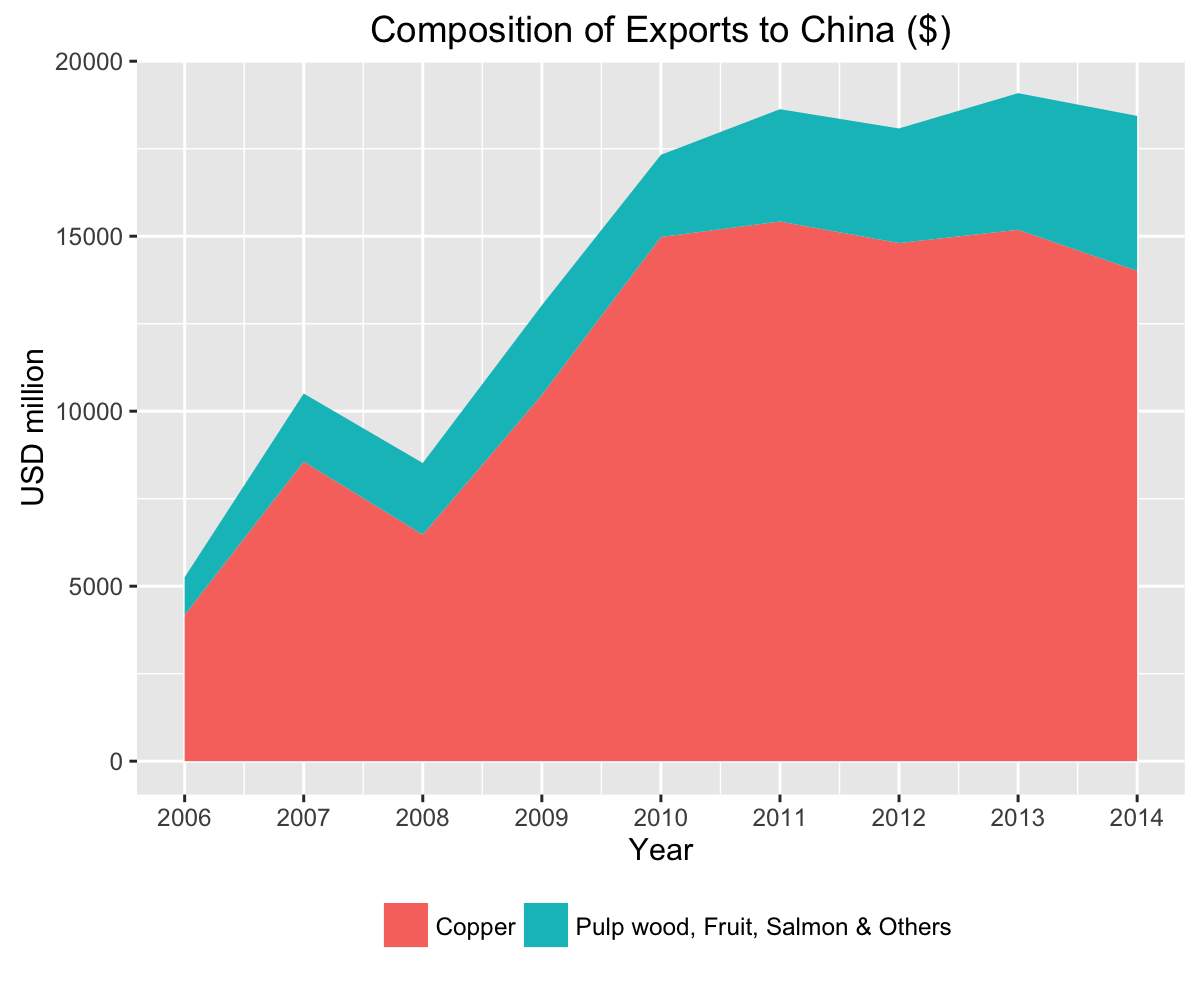
\includegraphics[width=0.55\linewidth]{0_all_posts_pdf/area_5-1} \end{center}

\section{Adjusting color palette}\label{adjusting-color-palette-1}

To change the colours, we use the \texttt{scale\_colour\_manual}
command. Note that you can reference the specific colours you'd like to
use with specific HEX codes. You can also reference colours by name,
with the full list of colours recognised by R
\href{http://www.stat.columbia.edu/~tzheng/files/Rcolor.pdf}{here}.

\begin{Shaded}
\begin{Highlighting}[]
\NormalTok{fill <-}\StringTok{ }\KeywordTok{c}\NormalTok{(}\StringTok{"#5F9EA0"}\NormalTok{, }\StringTok{"#E1B378"}\NormalTok{)}
\NormalTok{p2 <-}\StringTok{ }\NormalTok{p2 +}\StringTok{ }\KeywordTok{scale_fill_manual}\NormalTok{(}\DataTypeTok{values=}\NormalTok{fill)}
\NormalTok{p2}
\end{Highlighting}
\end{Shaded}

\begin{center}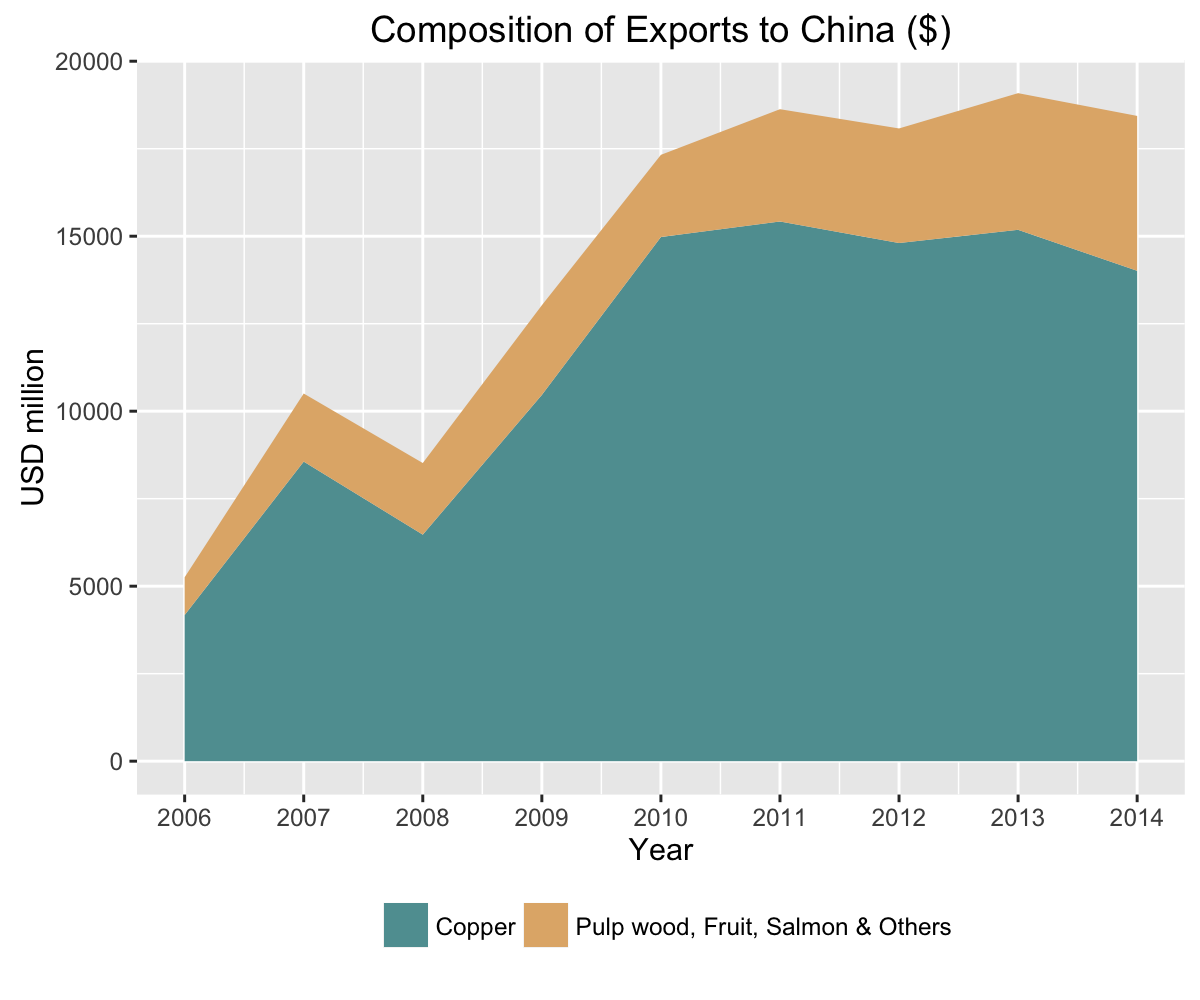
\includegraphics[width=0.55\linewidth]{0_all_posts_pdf/area_6-1} \end{center}

\section{Using the white theme}\label{using-the-white-theme-1}

As explained in the previous post, we can also change the overall look
of the site using themes. We'll start using a simple theme customisation
by adding \texttt{theme\_bw()} after \texttt{ggplot()}. As you can see,
we can further tweak the graph using the \texttt{theme} option, which
we've used so far to change the legend.

\begin{Shaded}
\begin{Highlighting}[]
\NormalTok{p2 <-}\StringTok{ }\KeywordTok{ggplot}\NormalTok{() +}
\StringTok{      }\KeywordTok{geom_area}\NormalTok{(}\KeywordTok{aes}\NormalTok{(}\DataTypeTok{y =} \NormalTok{export, }\DataTypeTok{x =} \NormalTok{year, }\DataTypeTok{fill =} \NormalTok{product), }\DataTypeTok{data =} \NormalTok{charts.data, }
\StringTok{        }\DataTypeTok{stat=}\StringTok{"identity"}\NormalTok{) +}\StringTok{ }
\StringTok{      }\KeywordTok{scale_x_continuous}\NormalTok{(}\DataTypeTok{breaks=}\KeywordTok{seq}\NormalTok{(}\DecValTok{2006}\NormalTok{,}\DecValTok{2014}\NormalTok{,}\DecValTok{1}\NormalTok{)) +}\StringTok{ }
\StringTok{      }\KeywordTok{labs}\NormalTok{(}\DataTypeTok{x=}\StringTok{"Year"}\NormalTok{, }\DataTypeTok{y=}\StringTok{"USD million"}\NormalTok{) +}\StringTok{ }
\StringTok{      }\KeywordTok{ggtitle}\NormalTok{(}\StringTok{"Composition of Exports to China ($)"}\NormalTok{) +}\StringTok{ }
\StringTok{      }\KeywordTok{scale_fill_manual}\NormalTok{(}\DataTypeTok{values=}\NormalTok{fill) +}
\StringTok{      }\KeywordTok{theme_bw}\NormalTok{() +}
\StringTok{      }\KeywordTok{theme}\NormalTok{(}\DataTypeTok{legend.position=}\StringTok{"bottom"}\NormalTok{, }
\StringTok{        }\DataTypeTok{legend.direction=}\StringTok{"horizontal"}\NormalTok{, }
\StringTok{        }\DataTypeTok{legend.title =} \KeywordTok{element_blank}\NormalTok{())   }
\NormalTok{p2}
\end{Highlighting}
\end{Shaded}

\begin{center}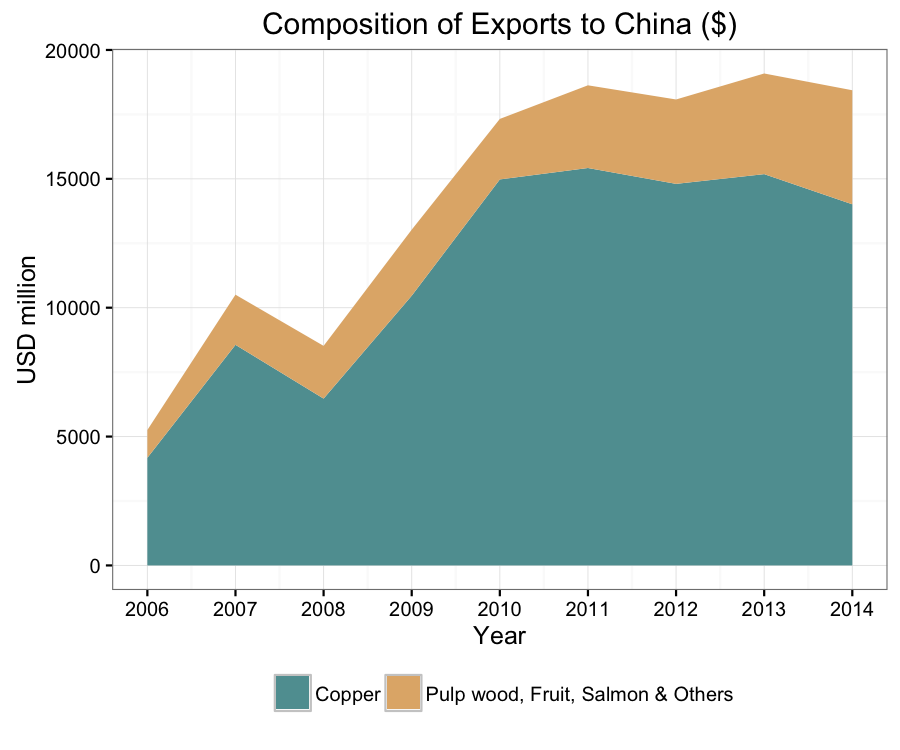
\includegraphics[width=0.55\linewidth]{0_all_posts_pdf/area_7-1} \end{center}

\section{Creating an XKCD style
chart}\label{creating-an-xkcd-style-chart-1}

Of course, you may want to create your own themes as well.
\texttt{ggplot2} allows for a very high degree of customisation,
including allowing you to use imported fonts. Below is an example of a
theme Mauricio was able to create which mimics the visual style of
\href{http://xkcd.com/}{XKCD}. In order to create this chart, you first
need to import the XKCD font, install it on your machine and load it
into R using the \texttt{extrafont} package. These instructions are
taken from
\href{https://www.google.com.au/url?sa=t\&rct=j\&q=\&esrc=s\&source=web\&cd=1\&ved=0ahUKEwiWzafchdPJAhVBpJQKHe_LDT8QFggbMAA\&url=https\%3A\%2F\%2Fcran.r-project.org\%2Fweb\%2Fpackages\%2Fxkcd\%2Fvignettes\%2Fxkcd-intro.pdf\&usg=AFQjCNE-KciGY14e-Q1buYIVmTFC0ht__Q\&sig2=DZUwkvIHwfNWtTtkcz94jg}{here}:

\begin{Shaded}
\begin{Highlighting}[]
\KeywordTok{library}\NormalTok{(extrafont)}

\KeywordTok{download.file}\NormalTok{(}\StringTok{"http://simonsoftware.se/other/xkcd.ttf"}\NormalTok{, }
\StringTok{      }\DataTypeTok{dest=}\StringTok{"xkcd.ttf"}\NormalTok{, }\DataTypeTok{mode=}\StringTok{"wb"}\NormalTok{)}
\KeywordTok{system}\NormalTok{(}\StringTok{"mkdir ~/.fonts"}\NormalTok{)}
\KeywordTok{system}\NormalTok{(}\StringTok{"cp xkcd.ttf  ~/.fonts"}\NormalTok{)}
\KeywordTok{font_import}\NormalTok{(}\DataTypeTok{paths =} \StringTok{"~/.fonts"}\NormalTok{, }\DataTypeTok{pattern=}\StringTok{"[X/x]kcd"}\NormalTok{)}
\KeywordTok{fonts}\NormalTok{()}
\KeywordTok{loadfonts}\NormalTok{()}
\end{Highlighting}
\end{Shaded}

You can then create your graph:

\begin{Shaded}
\begin{Highlighting}[]
\NormalTok{fill <-}\StringTok{ }\KeywordTok{c}\NormalTok{(}\StringTok{"#56B4E9"}\NormalTok{, }\StringTok{"#ffcc00"}\NormalTok{)}

\NormalTok{p2 <-}\StringTok{ }\KeywordTok{ggplot}\NormalTok{() +}\StringTok{ }
\StringTok{      }\KeywordTok{geom_area}\NormalTok{(}\KeywordTok{aes}\NormalTok{(}\DataTypeTok{y =} \NormalTok{export, }\DataTypeTok{x =} \NormalTok{year, }\DataTypeTok{fill =} \NormalTok{product), }\DataTypeTok{data =} \NormalTok{charts.data, }
\StringTok{        }\DataTypeTok{stat=}\StringTok{"identity"}\NormalTok{) +}\StringTok{ }
\StringTok{      }\KeywordTok{scale_x_continuous}\NormalTok{(}\DataTypeTok{breaks=}\KeywordTok{seq}\NormalTok{(}\DecValTok{2006}\NormalTok{,}\DecValTok{2014}\NormalTok{,}\DecValTok{1}\NormalTok{)) +}\StringTok{ }
\StringTok{      }\KeywordTok{labs}\NormalTok{(}\DataTypeTok{x=}\StringTok{"Year"}\NormalTok{, }\DataTypeTok{y=}\StringTok{"USD million"}\NormalTok{) +}\StringTok{ }
\StringTok{      }\KeywordTok{ggtitle}\NormalTok{(}\StringTok{"Composition of Exports to China ($)"}\NormalTok{) +}\StringTok{ }
\StringTok{      }\KeywordTok{scale_fill_manual}\NormalTok{(}\DataTypeTok{values=}\NormalTok{fill) +}\StringTok{ }
\StringTok{      }\KeywordTok{theme}\NormalTok{(}\DataTypeTok{axis.text.x=}\KeywordTok{element_text}\NormalTok{(}\DataTypeTok{colour=}\StringTok{"black"}\NormalTok{, }\DataTypeTok{size =} \DecValTok{10}\NormalTok{), }
\StringTok{        }\DataTypeTok{axis.text.y=}\KeywordTok{element_text}\NormalTok{(}\DataTypeTok{colour=}\StringTok{"black"}\NormalTok{, }\DataTypeTok{size =} \DecValTok{10}\NormalTok{),}
\StringTok{        }\DataTypeTok{axis.line.x =} \KeywordTok{element_line}\NormalTok{(}\DataTypeTok{size=}\NormalTok{.}\DecValTok{5}\NormalTok{, }\DataTypeTok{colour =} \StringTok{"black"}\NormalTok{),}
\StringTok{        }\DataTypeTok{axis.line.y =} \KeywordTok{element_line}\NormalTok{(}\DataTypeTok{size=}\NormalTok{.}\DecValTok{5}\NormalTok{, }\DataTypeTok{colour =} \StringTok{"black"}\NormalTok{),}
\StringTok{        }\DataTypeTok{legend.key=}\KeywordTok{element_rect}\NormalTok{(}\DataTypeTok{fill=}\StringTok{"white"}\NormalTok{, }\DataTypeTok{colour=}\StringTok{"white"}\NormalTok{),}
\StringTok{        }\DataTypeTok{legend.position=}\StringTok{"bottom"}\NormalTok{, }\DataTypeTok{legend.direction=}\StringTok{"horizontal"}\NormalTok{, }
\StringTok{        }\DataTypeTok{legend.title =} \KeywordTok{element_blank}\NormalTok{(),}
\StringTok{        }\DataTypeTok{panel.grid.major =} \KeywordTok{element_blank}\NormalTok{(),}
\StringTok{        }\DataTypeTok{panel.grid.minor =} \KeywordTok{element_blank}\NormalTok{(), }\DataTypeTok{panel.border =} \KeywordTok{element_blank}\NormalTok{(), }
\StringTok{        }\DataTypeTok{panel.background =} \KeywordTok{element_blank}\NormalTok{(),}
\StringTok{        }\DataTypeTok{plot.title=}\KeywordTok{element_text}\NormalTok{(}\DataTypeTok{family=}\StringTok{"xkcd-Regular"}\NormalTok{), }
\StringTok{        }\DataTypeTok{text=}\KeywordTok{element_text}\NormalTok{(}\DataTypeTok{family=}\StringTok{"xkcd-Regular"}\NormalTok{)) }
\NormalTok{p2}
\end{Highlighting}
\end{Shaded}

\begin{center}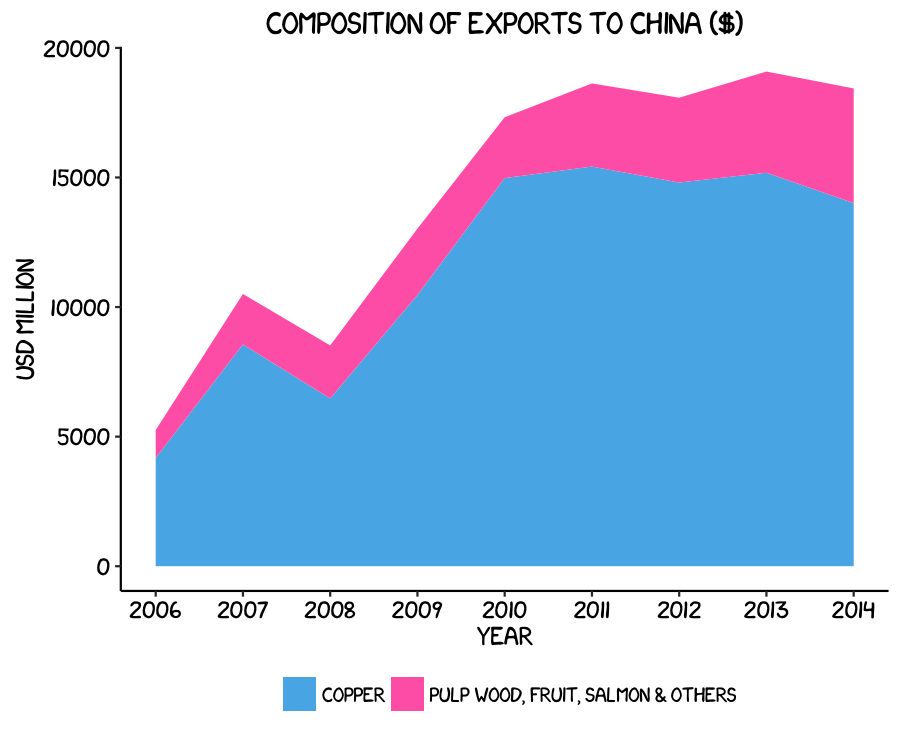
\includegraphics[width=0.55\linewidth]{0_all_posts_pdf/area_8-1} \end{center}

\section{\texorpdfstring{Using `The Economist'
theme}{Using The Economist theme}}\label{using-the-economist-theme-1}

There are a wider range of pre-built themes available as part of the
\texttt{ggthemes} package (more information on these
\href{https://cran.r-project.org/web/packages/ggthemes/vignettes/ggthemes.html}{here}).
Below we've applied \texttt{theme\_economist()}, which approximates
graphs in the Economist magazine. It is also important that the font
change argument inside \texttt{theme} is optional and it's only to
obtain a more similar result compared to the original. For an exact
result you need `Officina Sans' which is a commercial font and is
available \href{http://www.myfonts.com/fonts/itc/officina-sans/}{here}.

\begin{Shaded}
\begin{Highlighting}[]
\NormalTok{p2 <-}\StringTok{ }\KeywordTok{ggplot}\NormalTok{() +}
\StringTok{      }\KeywordTok{geom_area}\NormalTok{(}\KeywordTok{aes}\NormalTok{(}\DataTypeTok{y =} \NormalTok{export, }\DataTypeTok{x =} \NormalTok{year, }\DataTypeTok{fill =} \NormalTok{product), }\DataTypeTok{data =} \NormalTok{charts.data, }
\StringTok{        }\DataTypeTok{stat=}\StringTok{"identity"}\NormalTok{) +}\StringTok{ }
\StringTok{      }\KeywordTok{scale_x_continuous}\NormalTok{(}\DataTypeTok{breaks=}\KeywordTok{seq}\NormalTok{(}\DecValTok{2006}\NormalTok{,}\DecValTok{2014}\NormalTok{,}\DecValTok{1}\NormalTok{)) +}\StringTok{ }
\StringTok{      }\KeywordTok{labs}\NormalTok{(}\DataTypeTok{x=}\StringTok{"Year"}\NormalTok{, }\DataTypeTok{y=}\StringTok{"USD million"}\NormalTok{) +}\StringTok{ }
\StringTok{      }\KeywordTok{ggtitle}\NormalTok{(}\StringTok{"Composition of Exports to China ($)"}\NormalTok{) +}
\StringTok{      }\KeywordTok{theme_economist}\NormalTok{() +}\StringTok{ }\KeywordTok{scale_fill_economist}\NormalTok{() +}
\StringTok{      }\KeywordTok{theme}\NormalTok{(}\DataTypeTok{axis.line.x =} \KeywordTok{element_line}\NormalTok{(}\DataTypeTok{size=}\NormalTok{.}\DecValTok{5}\NormalTok{, }\DataTypeTok{colour =} \StringTok{"black"}\NormalTok{), }
\StringTok{        }\DataTypeTok{axis.line.y =} \KeywordTok{element_line}\NormalTok{(}\DataTypeTok{size=}\NormalTok{.}\DecValTok{5}\NormalTok{, }\DataTypeTok{colour =} \StringTok{"black"}\NormalTok{),}
\StringTok{        }\DataTypeTok{legend.position=}\StringTok{"bottom"}\NormalTok{, }
\StringTok{        }\DataTypeTok{legend.direction=}\StringTok{"horizontal"}\NormalTok{, }
\StringTok{        }\DataTypeTok{legend.title =} \KeywordTok{element_blank}\NormalTok{(),}
\StringTok{        }\DataTypeTok{plot.title=}\KeywordTok{element_text}\NormalTok{(}\DataTypeTok{family=}\StringTok{"OfficinaSanITC-Book"}\NormalTok{),}
\StringTok{        }\DataTypeTok{text=}\KeywordTok{element_text}\NormalTok{(}\DataTypeTok{family=}\StringTok{"OfficinaSanITC-Book"}\NormalTok{))   }
\NormalTok{p2}
\end{Highlighting}
\end{Shaded}

\begin{center}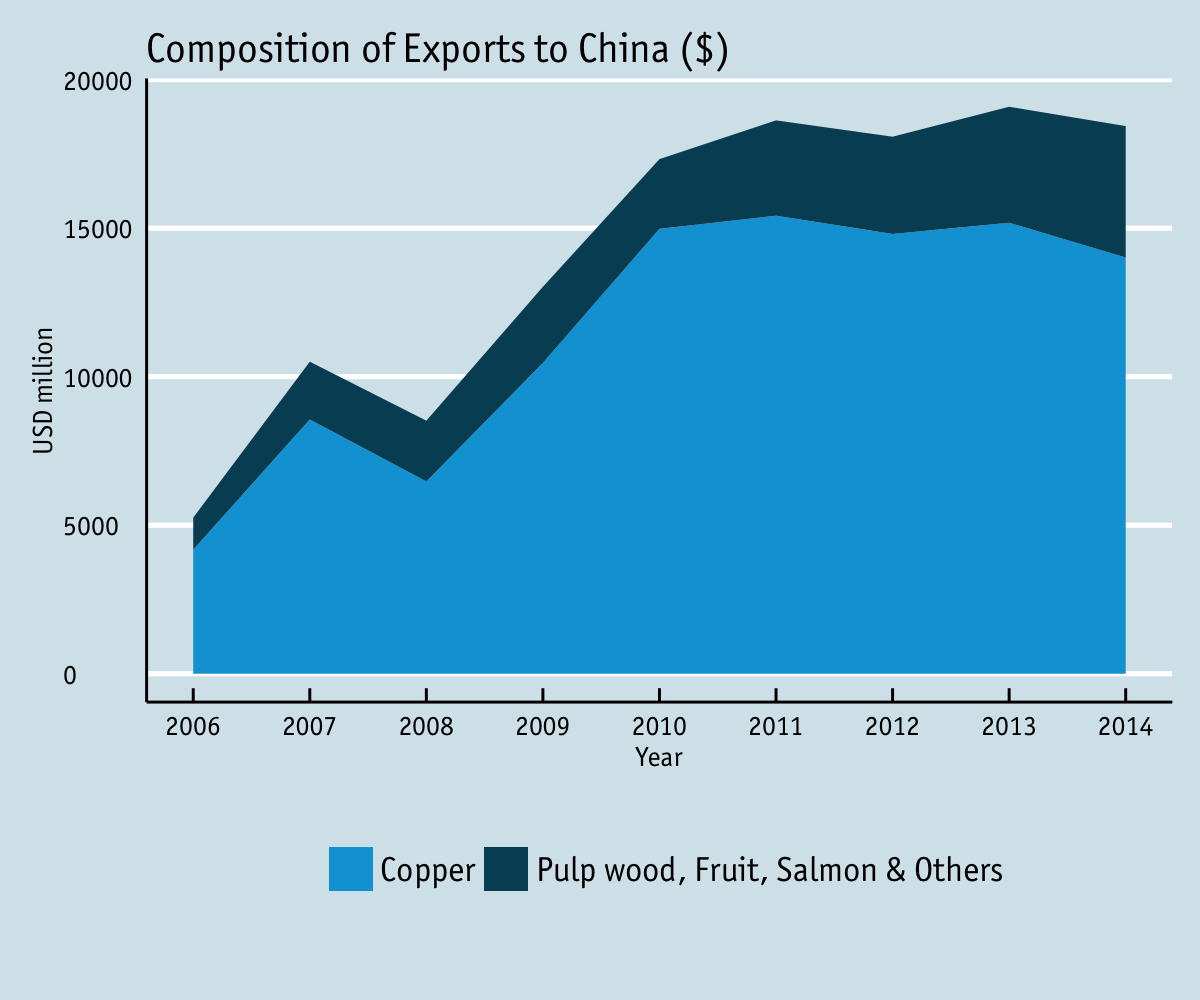
\includegraphics[width=0.55\linewidth]{0_all_posts_pdf/area_9-1} \end{center}

\section{Creating your own theme}\label{creating-your-own-theme-1}

As before, you can modify your plots a lot as \texttt{ggplot2} allows
many customisations. Here we present our original result shown at the
top of page.

\begin{Shaded}
\begin{Highlighting}[]
\NormalTok{fill <-}\StringTok{ }\KeywordTok{c}\NormalTok{(}\StringTok{"#40b8d0"}\NormalTok{, }\StringTok{"#b2d183"}\NormalTok{)}

\NormalTok{p2 <-}\StringTok{ }\KeywordTok{ggplot}\NormalTok{() +}\StringTok{ }
\StringTok{      }\KeywordTok{geom_area}\NormalTok{(}\KeywordTok{aes}\NormalTok{(}\DataTypeTok{y =} \NormalTok{export, }\DataTypeTok{x =} \NormalTok{year, }\DataTypeTok{fill =} \NormalTok{product), }\DataTypeTok{data =} \NormalTok{charts.data, }
\StringTok{        }\DataTypeTok{stat=}\StringTok{"identity"}\NormalTok{) +}\StringTok{ }
\StringTok{      }\KeywordTok{scale_x_continuous}\NormalTok{(}\DataTypeTok{breaks=}\KeywordTok{seq}\NormalTok{(}\DecValTok{2006}\NormalTok{,}\DecValTok{2014}\NormalTok{,}\DecValTok{1}\NormalTok{)) +}\StringTok{ }
\StringTok{      }\KeywordTok{labs}\NormalTok{(}\DataTypeTok{x=}\StringTok{"Year"}\NormalTok{, }\DataTypeTok{y=}\StringTok{"USD million"}\NormalTok{) +}\StringTok{ }
\StringTok{      }\KeywordTok{ggtitle}\NormalTok{(}\StringTok{"Composition of Exports to China ($)"}\NormalTok{) +}\StringTok{ }
\StringTok{      }\KeywordTok{scale_fill_manual}\NormalTok{(}\DataTypeTok{values=}\NormalTok{fill) +}\StringTok{ }
\StringTok{      }\KeywordTok{theme}\NormalTok{(}\DataTypeTok{axis.line.x =} \KeywordTok{element_line}\NormalTok{(}\DataTypeTok{size=}\NormalTok{.}\DecValTok{5}\NormalTok{, }\DataTypeTok{colour =} \StringTok{"black"}\NormalTok{), }
\StringTok{        }\DataTypeTok{axis.line.y =} \KeywordTok{element_line}\NormalTok{(}\DataTypeTok{size=}\NormalTok{.}\DecValTok{5}\NormalTok{, }\DataTypeTok{colour =} \StringTok{"black"}\NormalTok{), }
\StringTok{        }\DataTypeTok{axis.text.x=}\KeywordTok{element_text}\NormalTok{(}\DataTypeTok{colour=}\StringTok{"black"}\NormalTok{, }\DataTypeTok{size =} \DecValTok{10}\NormalTok{), }
\StringTok{        }\DataTypeTok{axis.text.y=}\KeywordTok{element_text}\NormalTok{(}\DataTypeTok{colour=}\StringTok{"black"}\NormalTok{, }\DataTypeTok{size =} \DecValTok{10}\NormalTok{),}
\StringTok{        }\DataTypeTok{legend.key=}\KeywordTok{element_rect}\NormalTok{(}\DataTypeTok{fill=}\StringTok{"white"}\NormalTok{, }\DataTypeTok{colour=}\StringTok{"white"}\NormalTok{),}
\StringTok{        }\DataTypeTok{legend.position=}\StringTok{"bottom"}\NormalTok{, }\DataTypeTok{legend.direction=}\StringTok{"horizontal"}\NormalTok{, }
\StringTok{        }\DataTypeTok{legend.title =} \KeywordTok{element_blank}\NormalTok{(),}
\StringTok{        }\DataTypeTok{panel.grid.major =} \KeywordTok{element_line}\NormalTok{(}\DataTypeTok{colour =} \StringTok{"#d3d3d3"}\NormalTok{), }
\StringTok{        }\DataTypeTok{panel.grid.minor =} \KeywordTok{element_blank}\NormalTok{(), }
\StringTok{        }\DataTypeTok{panel.border =} \KeywordTok{element_blank}\NormalTok{(), }
\StringTok{        }\DataTypeTok{panel.background =} \KeywordTok{element_blank}\NormalTok{(),}
\StringTok{        }\DataTypeTok{plot.title =} \KeywordTok{element_text}\NormalTok{(}\DataTypeTok{size =} \DecValTok{14}\NormalTok{, }\DataTypeTok{family =} \StringTok{"Tahoma"}\NormalTok{, }\DataTypeTok{face =} \StringTok{"bold"}\NormalTok{), }
\StringTok{        }\DataTypeTok{text=}\KeywordTok{element_text}\NormalTok{(}\DataTypeTok{family=}\StringTok{"Tahoma"}\NormalTok{))}
\NormalTok{p2}
\end{Highlighting}
\end{Shaded}

\begin{center}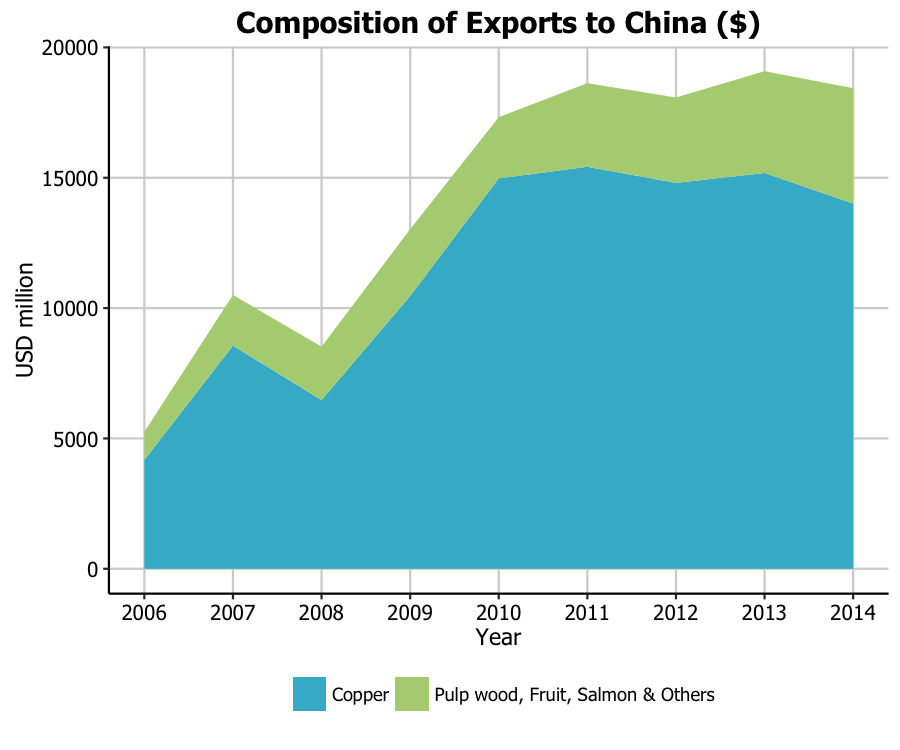
\includegraphics[width=0.55\linewidth]{0_all_posts_pdf/area_11-1} \end{center}
\chapter{Bar Plots}\label{bar-plots}

In this part, we will work towards creating the area plot below. We will
take you from a basic bar plot and explain all the customisations we add
to the code step-by-step.

\begin{center}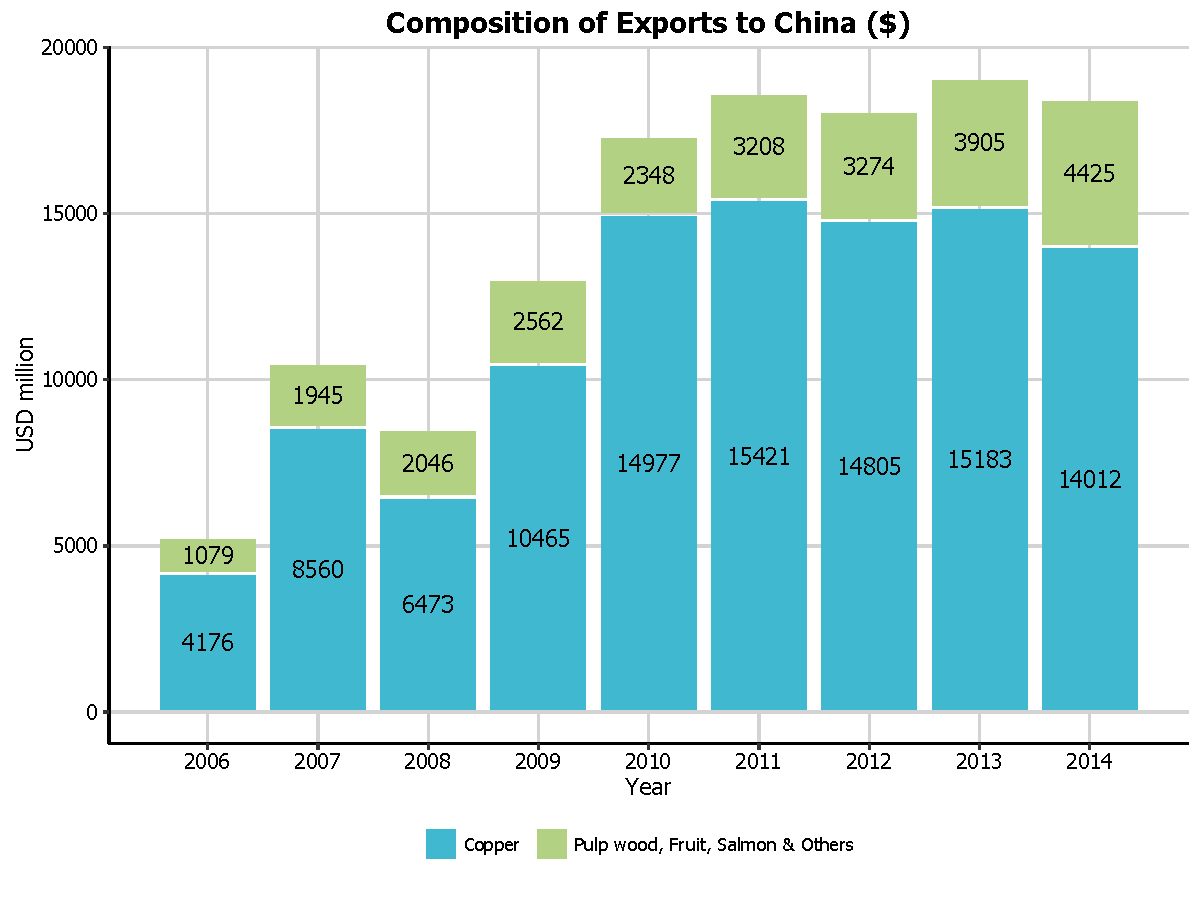
\includegraphics[width=0.55\linewidth]{figures/bar_final-1} \end{center}

We will use an international trade \href{http://pachamaltese.github.io/stats/trade-chile-china/copper-data-for-tutorial.csv}{dataset} made by ourselves from different sources (Chile Customs,
Central Bank of Chile and General Directorate of International Economic Relations).

\section{Basic graph}\label{basic-graph-2}

The first thing to do is load in the data and libraries, as below:

\begin{Shaded}
\begin{Highlighting}[]
\KeywordTok{library}\NormalTok{(ggplot2)}
\KeywordTok{library}\NormalTok{(ggthemes)}
\KeywordTok{library}\NormalTok{(extrafont)}
\KeywordTok{library}\NormalTok{(plyr)}
\KeywordTok{library}\NormalTok{(scales)}
\NormalTok{charts.data <-}\StringTok{ }\KeywordTok{read.csv}\NormalTok{(}\StringTok{"copper-data-for-tutorial.csv"}\NormalTok{)}
\end{Highlighting}
\end{Shaded}

In order to initialise a plot we tell ggplot that \texttt{charts.data}
is our data, and specify the variables on each axis. We then instruct
ggplot to render this as an bar plot by adding the \texttt{geom\_area}
command.

\begin{Shaded}
\begin{Highlighting}[]
\NormalTok{p3 <-}\StringTok{ }\KeywordTok{ggplot}\NormalTok{() +}\StringTok{ }\KeywordTok{geom_bar}\NormalTok{(}\KeywordTok{aes}\NormalTok{(}\DataTypeTok{y =} \NormalTok{export, }\DataTypeTok{x =} \NormalTok{year, }\DataTypeTok{fill =} \NormalTok{product), }
\StringTok{        }\DataTypeTok{data =} \NormalTok{charts.data, }\DataTypeTok{stat=}\StringTok{"identity"}\NormalTok{)}
\NormalTok{p3}
\end{Highlighting}
\end{Shaded}

\begin{center}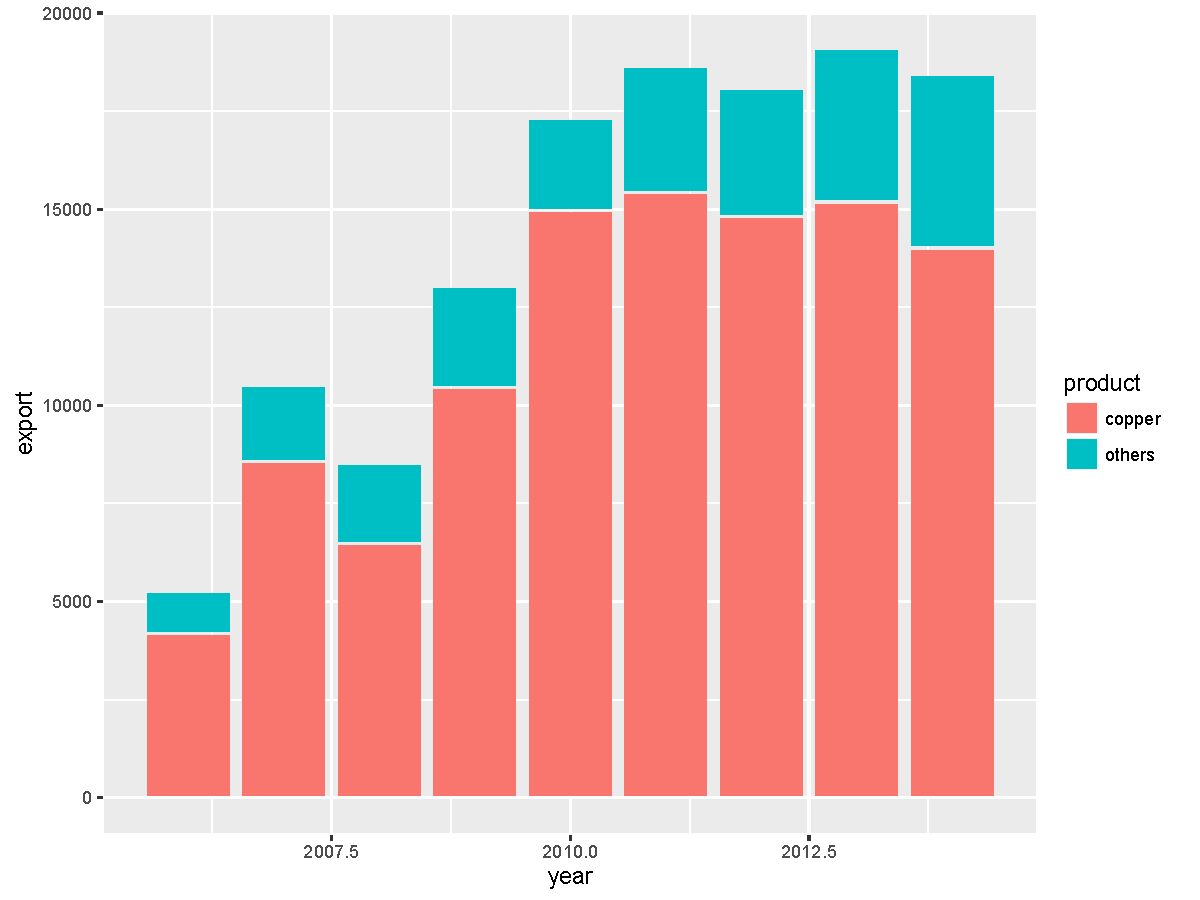
\includegraphics[width=0.55\linewidth]{figures/bar_1-1} \end{center}

\section{Adding data labels}\label{adding-data-labels}

To label the bars according to some variable in the data, we add the
\texttt{label} argument to the \texttt{ggplot(aes())} option. In this
case, we have labelled the bars with numbers from the \texttt{export}
variable.

\begin{Shaded}
\begin{Highlighting}[]
\NormalTok{p3 <-}\StringTok{ }\NormalTok{p3 +}\StringTok{ }\KeywordTok{geom_text}\NormalTok{(}\DataTypeTok{data=}\NormalTok{charts.data, }\KeywordTok{aes}\NormalTok{(}\DataTypeTok{x =} \NormalTok{year, }\DataTypeTok{y =} \NormalTok{export, }
\StringTok{        }\DataTypeTok{label =} \NormalTok{export), }\DataTypeTok{size=}\DecValTok{4}\NormalTok{)}
\NormalTok{p3}
\end{Highlighting}
\end{Shaded}

\begin{center}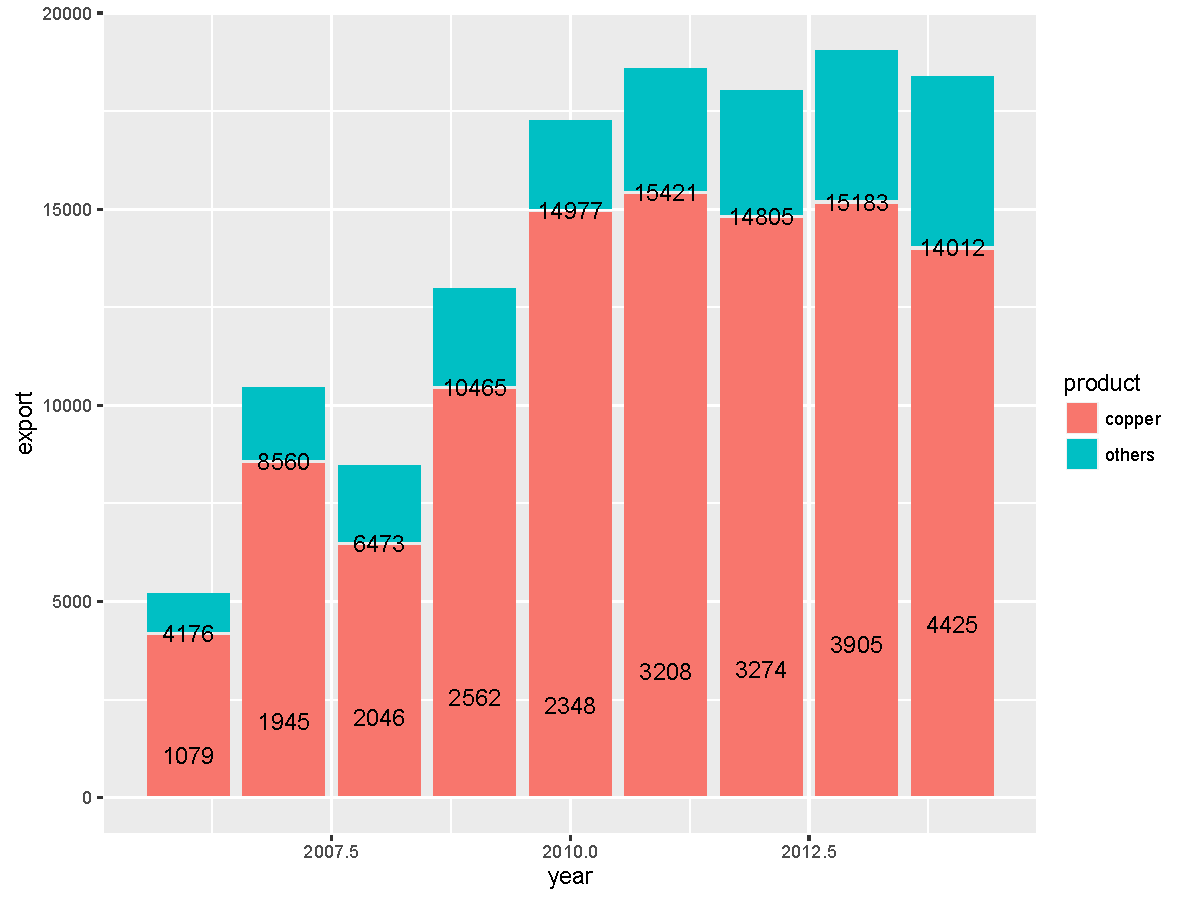
\includegraphics[width=0.55\linewidth]{figures/bar_2-1} \end{center}

\section{Adjusting data labels
position}\label{adjusting-data-labels-position}

To adjust the position of the data labels from the default placement, we
use the \texttt{ddply} function on the data, and create a new variable
called \texttt{pos}. This variable is at the centre of each bar and can
be used to specify the position of the labels by assigning it to the
\texttt{y} argument in \texttt{geom\_text(aes())}.

\begin{Shaded}
\begin{Highlighting}[]
\NormalTok{charts.data <-}\StringTok{ }\KeywordTok{ddply}\NormalTok{(charts.data, .(year), transform, }
\StringTok{        }\DataTypeTok{pos =} \KeywordTok{cumsum}\NormalTok{(export) -}\StringTok{ }\NormalTok{(}\FloatTok{0.5} \NormalTok{*}\StringTok{ }\NormalTok{export))}

\NormalTok{p3 <-}\StringTok{ }\KeywordTok{ggplot}\NormalTok{() +}\StringTok{ }\KeywordTok{geom_bar}\NormalTok{(}\KeywordTok{aes}\NormalTok{(}\DataTypeTok{y =} \NormalTok{export, }\DataTypeTok{x =} \NormalTok{year, }\DataTypeTok{fill =} \NormalTok{product), }
\StringTok{        }\DataTypeTok{data =} \NormalTok{charts.data, }\DataTypeTok{stat=}\StringTok{"identity"}\NormalTok{) }
\NormalTok{p3 <-}\StringTok{ }\NormalTok{p3 +}\StringTok{ }\KeywordTok{geom_text}\NormalTok{(}\StringTok{        }\DataTypeTok{data=}\NormalTok{charts.data, }\KeywordTok{aes}\NormalTok{(}\DataTypeTok{x =} \NormalTok{year, }\DataTypeTok{y =} \NormalTok{pos, }\DataTypeTok{label =} \NormalTok{export), }
\StringTok{        }\DataTypeTok{size=}\DecValTok{4}\NormalTok{)}
\NormalTok{p3}
\end{Highlighting}
\end{Shaded}

\begin{center}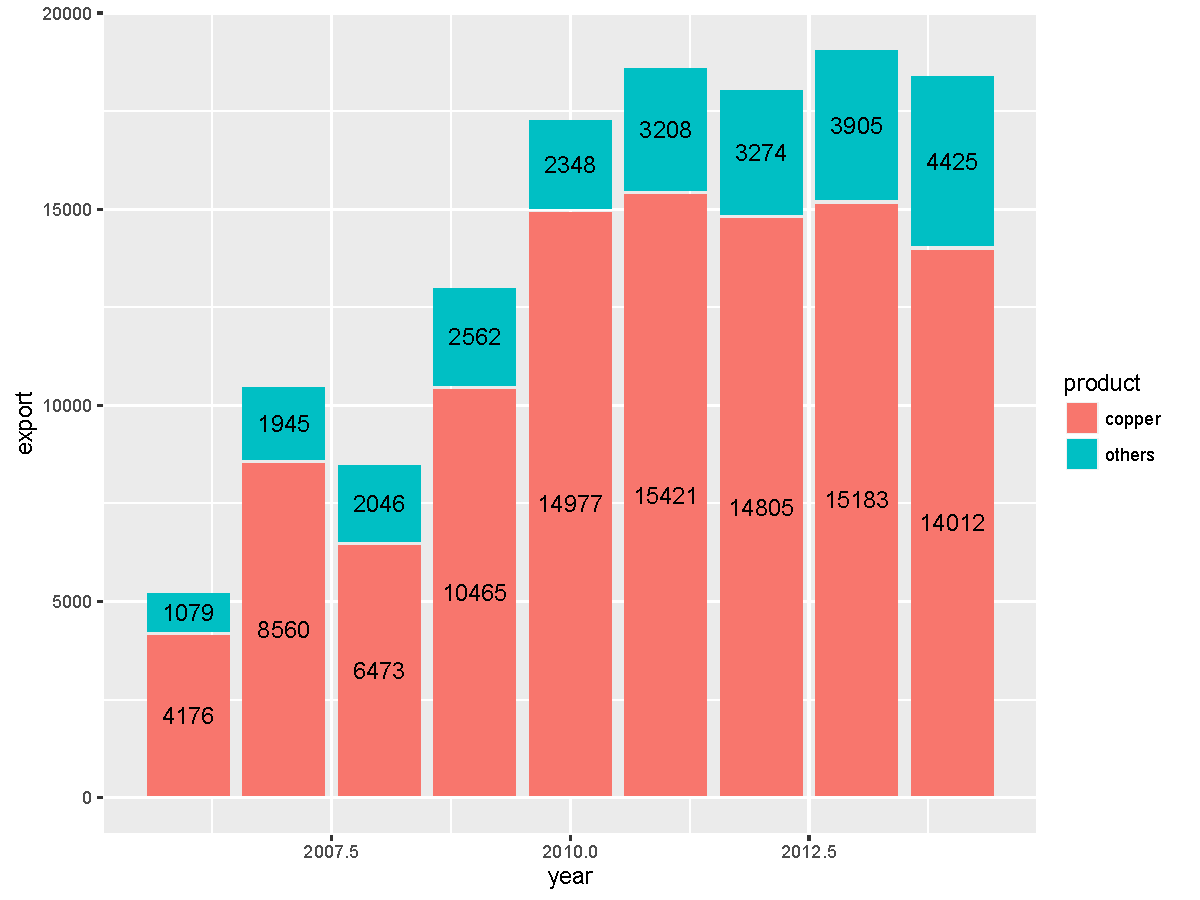
\includegraphics[width=0.55\linewidth]{figures/bar_3-1} \end{center}

\section{Adjusting legend
position}\label{adjusting-legend-position-1}

To adjust the position of the legend from the default spot of right of
the graph, we add the \texttt{theme} option and specify the
\texttt{legend.position="bottom"} argument. We can also change the title
to blank using the \texttt{legend.title\ =\ element\_blank()} argument
and change the legend shape using the
\texttt{legend.direction="horizontal"} argument.

\begin{Shaded}
\begin{Highlighting}[]
\NormalTok{p3 <-}\StringTok{ }\NormalTok{p3 +}\StringTok{ }\KeywordTok{theme}\NormalTok{(}\DataTypeTok{legend.position=}\StringTok{"bottom"}\NormalTok{, }\DataTypeTok{legend.direction=}\StringTok{"horizontal"}\NormalTok{, }
\StringTok{        }\DataTypeTok{legend.title =} \KeywordTok{element_blank}\NormalTok{())}
\NormalTok{p3}
\end{Highlighting}
\end{Shaded}

\begin{center}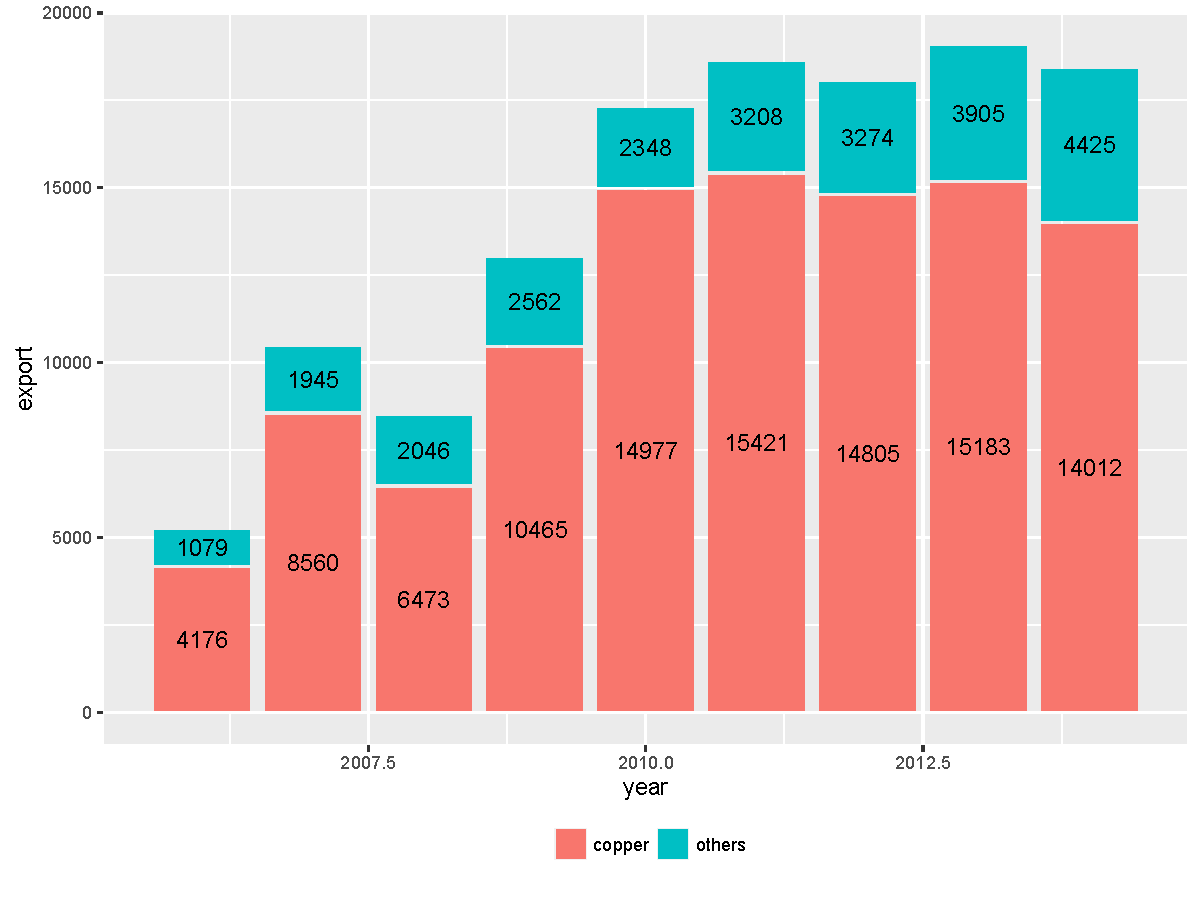
\includegraphics[width=0.55\linewidth]{figures/bar_4-1} \end{center}

\section{Changing variables
display}\label{changing-variables-display-2}

To change the variables' displayed name, we need to re-factor our data
labels in \texttt{charts.data} data frame.

\begin{Shaded}
\begin{Highlighting}[]
\NormalTok{charts.data$product <-}\StringTok{ }\KeywordTok{factor}\NormalTok{(charts.data$product, }
\StringTok{        }\DataTypeTok{levels =} \KeywordTok{c}\NormalTok{(}\StringTok{"copper"}\NormalTok{,}\StringTok{"others"}\NormalTok{), }
\StringTok{        }\DataTypeTok{labels =} \KeywordTok{c}\NormalTok{(}\StringTok{"Copper"}\NormalTok{,}\StringTok{"Pulp wood, Fruit, Salmon & Others"}\NormalTok{))}

\NormalTok{p3 <-}\StringTok{ }\KeywordTok{ggplot}\NormalTok{() +}\StringTok{ }\KeywordTok{geom_bar}\NormalTok{(}\KeywordTok{aes}\NormalTok{(}\DataTypeTok{y =} \NormalTok{export, }\DataTypeTok{x =} \NormalTok{year, }\DataTypeTok{fill =} \NormalTok{product), }
\StringTok{        }\DataTypeTok{data =} \NormalTok{charts.data, }\DataTypeTok{stat=}\StringTok{"identity"}\NormalTok{) +}\StringTok{ }
\StringTok{      }\KeywordTok{geom_text}\NormalTok{(}\DataTypeTok{data=}\NormalTok{charts.data, }\KeywordTok{aes}\NormalTok{(}\DataTypeTok{x =} \NormalTok{year, }\DataTypeTok{y =} \NormalTok{pos, }\DataTypeTok{label =} \NormalTok{export, }
\StringTok{        }\DataTypeTok{size=}\DecValTok{4}\NormalTok{), }\DataTypeTok{show.legend =} \NormalTok{F) +}\StringTok{ }
\StringTok{      }\KeywordTok{theme}\NormalTok{(}\DataTypeTok{legend.position=}\StringTok{"bottom"}\NormalTok{, }\DataTypeTok{legend.direction=}\StringTok{"horizontal"}\NormalTok{, }
\StringTok{        }\DataTypeTok{legend.title =} \KeywordTok{element_blank}\NormalTok{())}
\NormalTok{p3}
\end{Highlighting}
\end{Shaded}

\begin{center}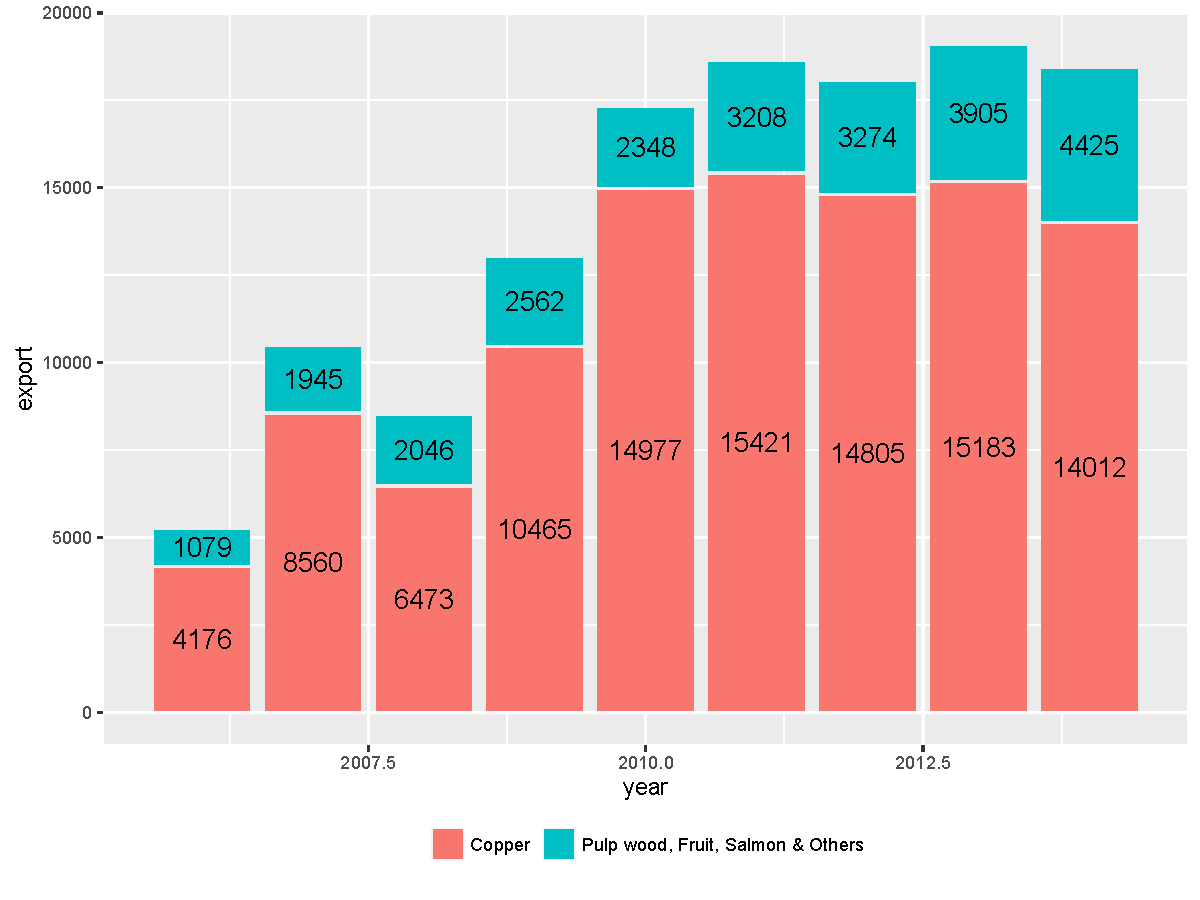
\includegraphics[width=0.55\linewidth]{figures/bar_5-1} \end{center}

\section{Adjusting x-axis scale}\label{adjusting-x-axis-scale-2}

To change the axis tick marks, we use the \texttt{scale\_x\_continuous}
and/or \texttt{scale\_y\_continuous} commands.

\begin{Shaded}
\begin{Highlighting}[]
\NormalTok{p3 <-}\StringTok{ }\NormalTok{p3 +}\StringTok{ }\KeywordTok{scale_x_continuous}\NormalTok{(}\DataTypeTok{breaks=}\KeywordTok{seq}\NormalTok{(}\DecValTok{2006}\NormalTok{,}\DecValTok{2014}\NormalTok{,}\DecValTok{1}\NormalTok{))}
\NormalTok{p3}
\end{Highlighting}
\end{Shaded}

\begin{center}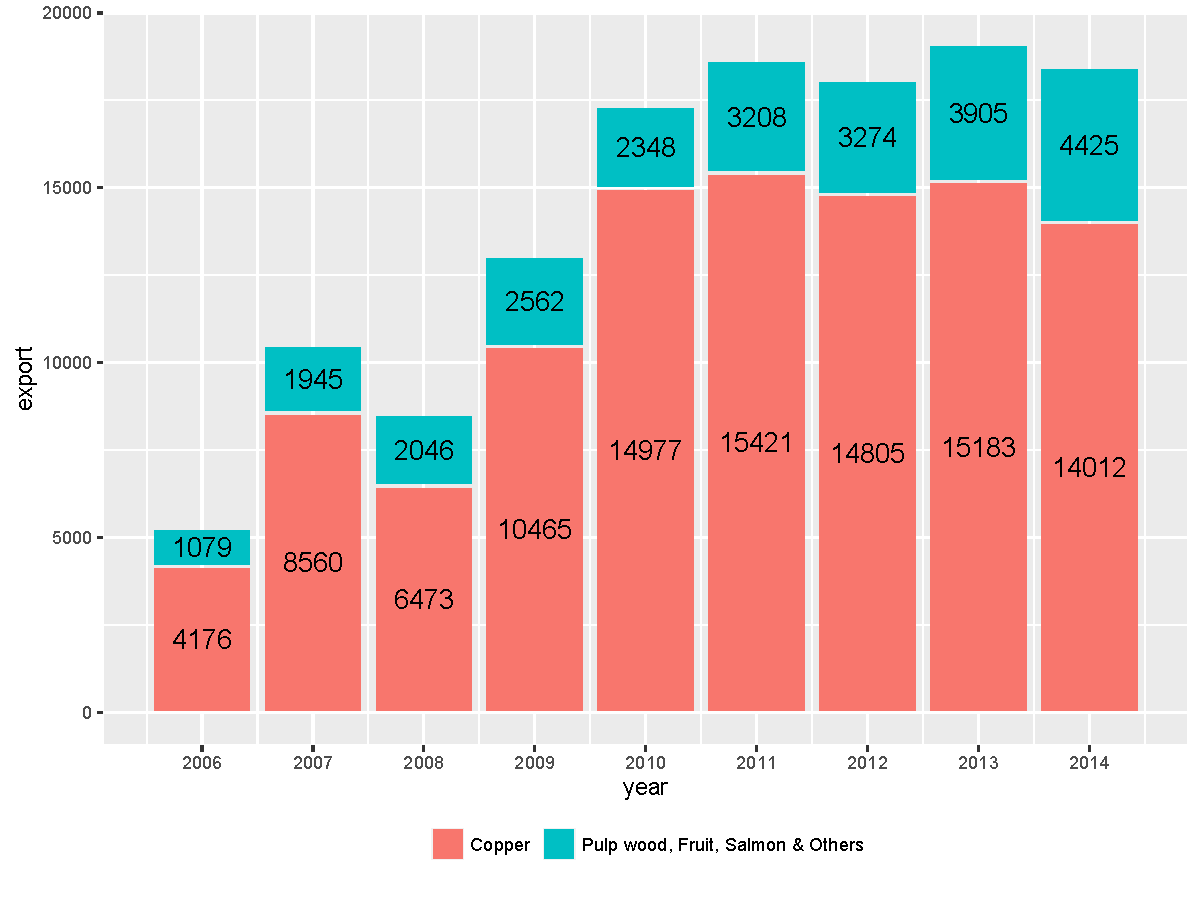
\includegraphics[width=0.55\linewidth]{figures/bar_6-1} \end{center}

\section{Adjusting axis labels \& adding
title}\label{adjusting-axis-labels-adding-title-2}

To add a title, we include the option \texttt{ggtitle} and include the
name of the graph as a string argument, and to change the axis names we
use the \texttt{labs} command.

\begin{Shaded}
\begin{Highlighting}[]
\NormalTok{p3 <-}\StringTok{ }\NormalTok{p3 +}\StringTok{ }\KeywordTok{ggtitle}\NormalTok{(}\StringTok{"Composition of Exports to China ($)"}\NormalTok{) +}\StringTok{ }
\StringTok{      }\KeywordTok{labs}\NormalTok{(}\DataTypeTok{x=}\StringTok{"Year"}\NormalTok{, }\DataTypeTok{y=}\StringTok{"USD million"}\NormalTok{) }
\NormalTok{p3}
\end{Highlighting}
\end{Shaded}

\begin{center}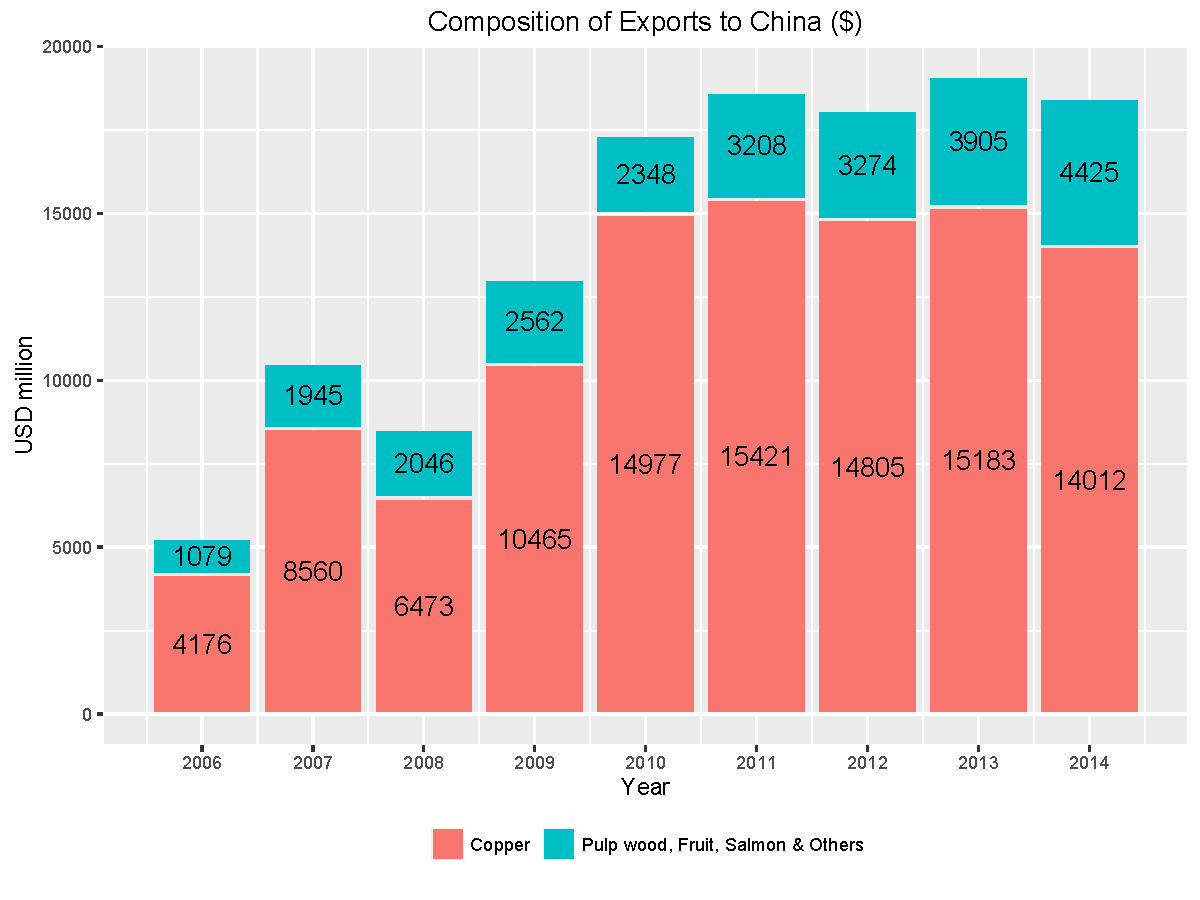
\includegraphics[width=0.55\linewidth]{figures/bar_7-1} \end{center}

\section{Adjusting color palette}\label{adjusting-color-palette-2}

To change the colours, we use the \texttt{scale\_colour\_manual}
command. Note that you can reference the specific colours you'd like to
use with specific HEX codes. You can also reference colours by name,
with the full list of colours recognised by R
\href{http://www.stat.columbia.edu/~tzheng/files/Rcolor.pdf}{here}.

\begin{Shaded}
\begin{Highlighting}[]
\NormalTok{fill <-}\StringTok{ }\KeywordTok{c}\NormalTok{(}\StringTok{"#5F9EA0"}\NormalTok{, }\StringTok{"#E1B378"}\NormalTok{)}
\NormalTok{p3 <-}\StringTok{ }\NormalTok{p3 +}\StringTok{ }\KeywordTok{scale_fill_manual}\NormalTok{(}\DataTypeTok{values=}\NormalTok{fill)}
\NormalTok{p3}
\end{Highlighting}
\end{Shaded}

\begin{center}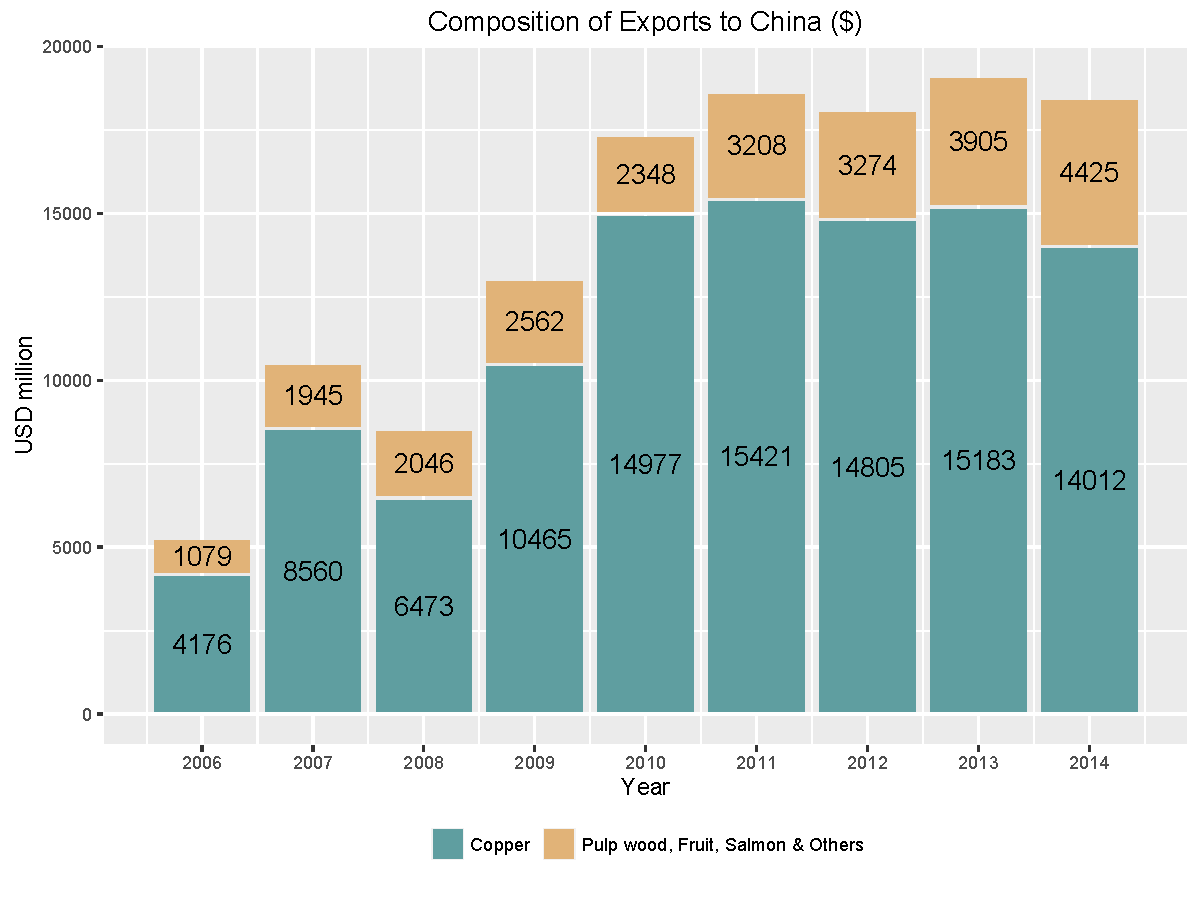
\includegraphics[width=0.55\linewidth]{figures/bar_8-1} \end{center}

\section{Using the white theme}\label{using-the-white-theme-2}

As explained in the previous posts, we can also change the overall look
of the graph using themes. We'll start using a simple theme
customisation by adding \texttt{theme\_bw()} after \texttt{ggplot()}. As
you can see, we can further tweak the graph using the \texttt{theme}
option, which we've used so far to change the legend.

\begin{Shaded}
\begin{Highlighting}[]
\NormalTok{p3 <-}\StringTok{ }\KeywordTok{ggplot}\NormalTok{() +}
\StringTok{      }\KeywordTok{geom_bar}\NormalTok{(}\KeywordTok{aes}\NormalTok{(}\DataTypeTok{y =} \NormalTok{export, }\DataTypeTok{x =} \NormalTok{year, }\DataTypeTok{fill =} \NormalTok{product), }\DataTypeTok{data =} \NormalTok{charts.data, }
\StringTok{        }\DataTypeTok{stat=}\StringTok{"identity"}\NormalTok{) +}\StringTok{ }
\StringTok{      }\KeywordTok{geom_text}\NormalTok{(}\DataTypeTok{data=}\NormalTok{charts.data, }\KeywordTok{aes}\NormalTok{(}\DataTypeTok{x =} \NormalTok{year, }\DataTypeTok{y =} \NormalTok{pos, }\DataTypeTok{label =} \NormalTok{export, }
\StringTok{        }\DataTypeTok{size=}\DecValTok{4}\NormalTok{), }\DataTypeTok{show.legend =} \NormalTok{F) +}\StringTok{ }
\StringTok{      }\KeywordTok{scale_x_continuous}\NormalTok{(}\DataTypeTok{breaks=}\KeywordTok{seq}\NormalTok{(}\DecValTok{2006}\NormalTok{,}\DecValTok{2014}\NormalTok{,}\DecValTok{1}\NormalTok{)) +}\StringTok{ }
\StringTok{      }\KeywordTok{labs}\NormalTok{(}\DataTypeTok{x=}\StringTok{"Year"}\NormalTok{, }\DataTypeTok{y=}\StringTok{"USD million"}\NormalTok{) +}\StringTok{ }
\StringTok{      }\KeywordTok{ggtitle}\NormalTok{(}\StringTok{"Composition of Exports to China ($)"}\NormalTok{) +}\StringTok{ }
\StringTok{      }\KeywordTok{scale_fill_manual}\NormalTok{(}\DataTypeTok{values=}\NormalTok{fill) +}
\StringTok{      }\KeywordTok{theme_bw}\NormalTok{() +}
\StringTok{      }\KeywordTok{theme}\NormalTok{(}\DataTypeTok{legend.position=}\StringTok{"bottom"}\NormalTok{, }
        \DataTypeTok{legend.direction=}\StringTok{"horizontal"}\NormalTok{, }
        \DataTypeTok{legend.title =} \KeywordTok{element_blank}\NormalTok{())   }
\NormalTok{p3}
\end{Highlighting}
\end{Shaded}

\begin{center}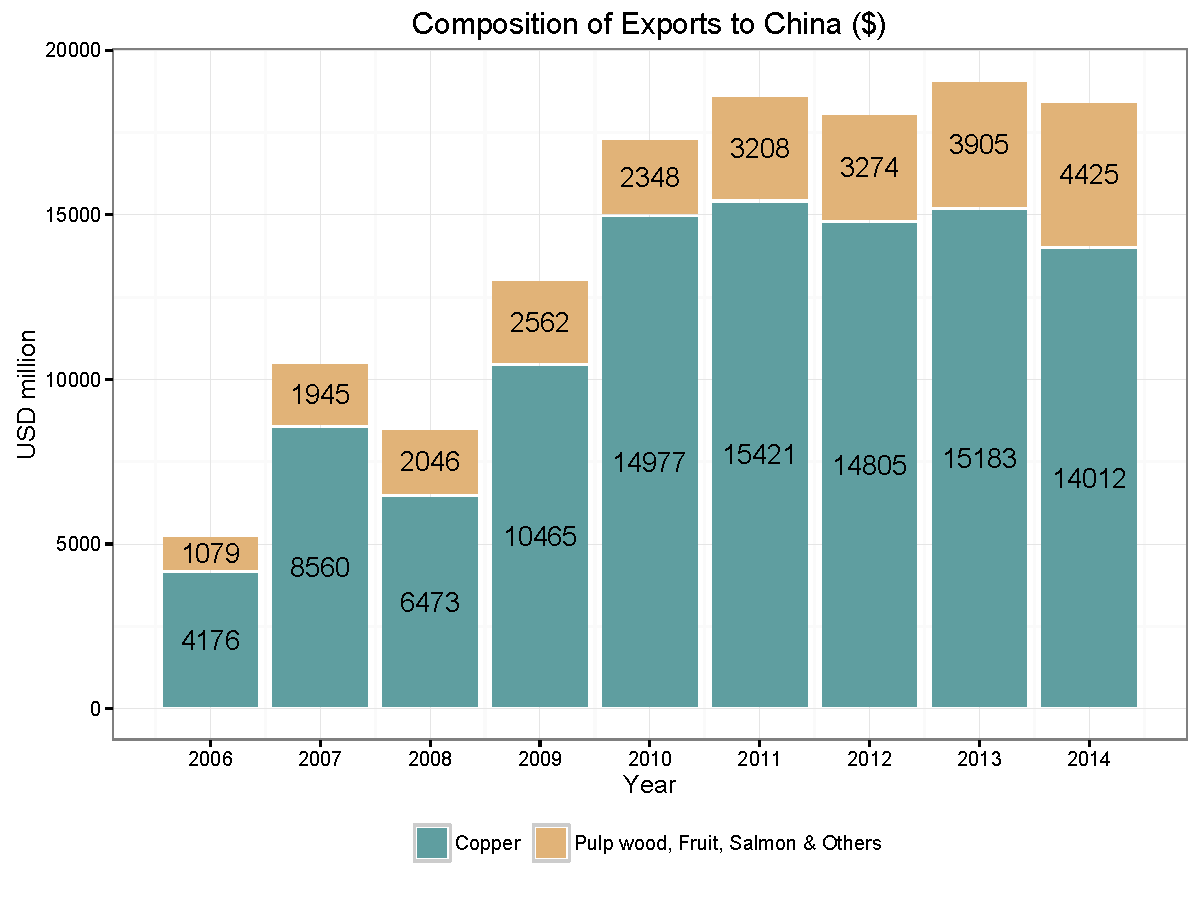
\includegraphics[width=0.55\linewidth]{figures/bar_9-1} \end{center}

\section{Creating an XKCD style
chart}\label{creating-an-xkcd-style-chart-2}

Of course, you may want to create your own themes as well.
\texttt{ggplot2} allows for a very high degree of customisation,
including allowing you to use imported fonts. Below is an example of a
theme Mauricio was able to create which mimics the visual style of
\href{http://xkcd.com/}{XKCD}. In order to create this chart, you first
need to import the XKCD font, install it on your machine and load it
into R using the \texttt{extrafont} package. These instructions are
taken from
\href{https://www.google.com.au/url?sa=t\&rct=j\&q=\&esrc=s\&source=web\&cd=1\&ved=0ahUKEwiWzafchdPJAhVBpJQKHe_LDT8QFggbMAA\&url=https\%3A\%2F\%2Fcran.r-project.org\%2Fweb\%2Fpackages\%2Fxkcd\%2Fvignettes\%2Fxkcd-intro.pdf\&usg=AFQjCNE-KciGY14e-Q1buYIVmTFC0ht__Q\&sig2=DZUwkvIHwfNWtTtkcz94jg}{here}:

\begin{Shaded}
\begin{Highlighting}[]
\KeywordTok{library}\NormalTok{(extrafont)}

\KeywordTok{download.file}\NormalTok{(}\StringTok{"http://simonsoftware.se/other/xkcd.ttf"}\NormalTok{, }
\StringTok{      }\DataTypeTok{dest=}\StringTok{"xkcd.ttf"}\NormalTok{, }\DataTypeTok{mode=}\StringTok{"wb"}\NormalTok{)}
\KeywordTok{system}\NormalTok{(}\StringTok{"mkdir ~/.fonts"}\NormalTok{)}
\KeywordTok{system}\NormalTok{(}\StringTok{"cp xkcd.ttf  ~/.fonts"}\NormalTok{)}
\KeywordTok{font_import}\NormalTok{(}\DataTypeTok{paths =} \StringTok{"~/.fonts"}\NormalTok{, }\DataTypeTok{pattern=}\StringTok{"[X/x]kcd"}\NormalTok{)}
\KeywordTok{fonts}\NormalTok{()}
\KeywordTok{loadfonts}\NormalTok{()}
\end{Highlighting}
\end{Shaded}

You can then create your graph:

\begin{Shaded}
\begin{Highlighting}[]
\NormalTok{fill <-}\StringTok{ }\KeywordTok{c}\NormalTok{(}\StringTok{"#56B4E9"}\NormalTok{, }\StringTok{"#F0E442"}\NormalTok{)}

\NormalTok{p3 <-}\StringTok{ }\KeywordTok{ggplot}\NormalTok{() +}\StringTok{ }
\StringTok{      }\KeywordTok{geom_bar}\NormalTok{(}\KeywordTok{aes}\NormalTok{(}\DataTypeTok{y =} \NormalTok{export, }\DataTypeTok{x =} \NormalTok{year, }\DataTypeTok{fill =} \NormalTok{product), }\DataTypeTok{data =} \NormalTok{charts.data, }
\StringTok{        }\DataTypeTok{stat=}\StringTok{"identity"}\NormalTok{) +}\StringTok{ }
\StringTok{      }\KeywordTok{geom_text}\NormalTok{(}\DataTypeTok{data=}\NormalTok{charts.data, }\KeywordTok{aes}\NormalTok{(}\DataTypeTok{x =} \NormalTok{year, }\DataTypeTok{y =} \NormalTok{pos, }\DataTypeTok{label =} \NormalTok{export), }
\StringTok{        }\DataTypeTok{colour=}\StringTok{"black"}\NormalTok{, }\DataTypeTok{family=}\StringTok{"xkcd-Regular"}\NormalTok{, }\DataTypeTok{size =} \DecValTok{4}\NormalTok{, }\DataTypeTok{show.legend =} \NormalTok{F) +}\StringTok{ }
\StringTok{      }\KeywordTok{scale_x_continuous}\NormalTok{(}\DataTypeTok{breaks=}\KeywordTok{seq}\NormalTok{(}\DecValTok{2006}\NormalTok{,}\DecValTok{2014}\NormalTok{,}\DecValTok{1}\NormalTok{)) +}\StringTok{ }
\StringTok{      }\KeywordTok{labs}\NormalTok{(}\DataTypeTok{x=}\StringTok{"Year"}\NormalTok{, }\DataTypeTok{y=}\StringTok{"USD million"}\NormalTok{) +}\StringTok{ }
\StringTok{      }\KeywordTok{ggtitle}\NormalTok{(}\StringTok{"Composition of Exports to China ($)"}\NormalTok{) +}\StringTok{ }
\StringTok{      }\KeywordTok{scale_fill_manual}\NormalTok{(}\DataTypeTok{values=}\NormalTok{fill) +}\StringTok{ }
\StringTok{      }\KeywordTok{theme}\NormalTok{(}\DataTypeTok{axis.text.x=}\KeywordTok{element_text}\NormalTok{(}\DataTypeTok{colour=}\StringTok{"black"}\NormalTok{, }\DataTypeTok{size =} \DecValTok{10}\NormalTok{), }
        \DataTypeTok{axis.text.y=}\KeywordTok{element_text}\NormalTok{(}\DataTypeTok{colour=}\StringTok{"black"}\NormalTok{, }\DataTypeTok{size =} \DecValTok{10}\NormalTok{),}
        \DataTypeTok{axis.line.x =} \KeywordTok{element_line}\NormalTok{(}\DataTypeTok{size=}\NormalTok{.}\DecValTok{5}\NormalTok{, }\DataTypeTok{colour =} \StringTok{"black"}\NormalTok{),}
        \DataTypeTok{axis.line.y =} \KeywordTok{element_line}\NormalTok{(}\DataTypeTok{size=}\NormalTok{.}\DecValTok{5}\NormalTok{, }\DataTypeTok{colour =} \StringTok{"black"}\NormalTok{),}
        \DataTypeTok{legend.key=}\KeywordTok{element_rect}\NormalTok{(}\DataTypeTok{fill=}\StringTok{"white"}\NormalTok{, }\DataTypeTok{colour=}\StringTok{"white"}\NormalTok{),}
        \DataTypeTok{legend.position=}\StringTok{"bottom"}\NormalTok{, }\DataTypeTok{legend.direction=}\StringTok{"horizontal"}\NormalTok{, }
        \DataTypeTok{legend.title =} \KeywordTok{element_blank}\NormalTok{(),}
        \DataTypeTok{panel.grid.major =} \KeywordTok{element_blank}\NormalTok{(),}
        \DataTypeTok{panel.grid.minor =} \KeywordTok{element_blank}\NormalTok{(), }\DataTypeTok{panel.border =} \KeywordTok{element_blank}\NormalTok{(), }
        \DataTypeTok{panel.background =} \KeywordTok{element_blank}\NormalTok{(),}
        \DataTypeTok{plot.title=}\KeywordTok{element_text}\NormalTok{(}\DataTypeTok{family=}\StringTok{"xkcd-Regular"}\NormalTok{), }
        \DataTypeTok{text=}\KeywordTok{element_text}\NormalTok{(}\DataTypeTok{family=}\StringTok{"xkcd-Regular"}\NormalTok{)) }
\NormalTok{p3}
\end{Highlighting}
\end{Shaded}

\begin{center}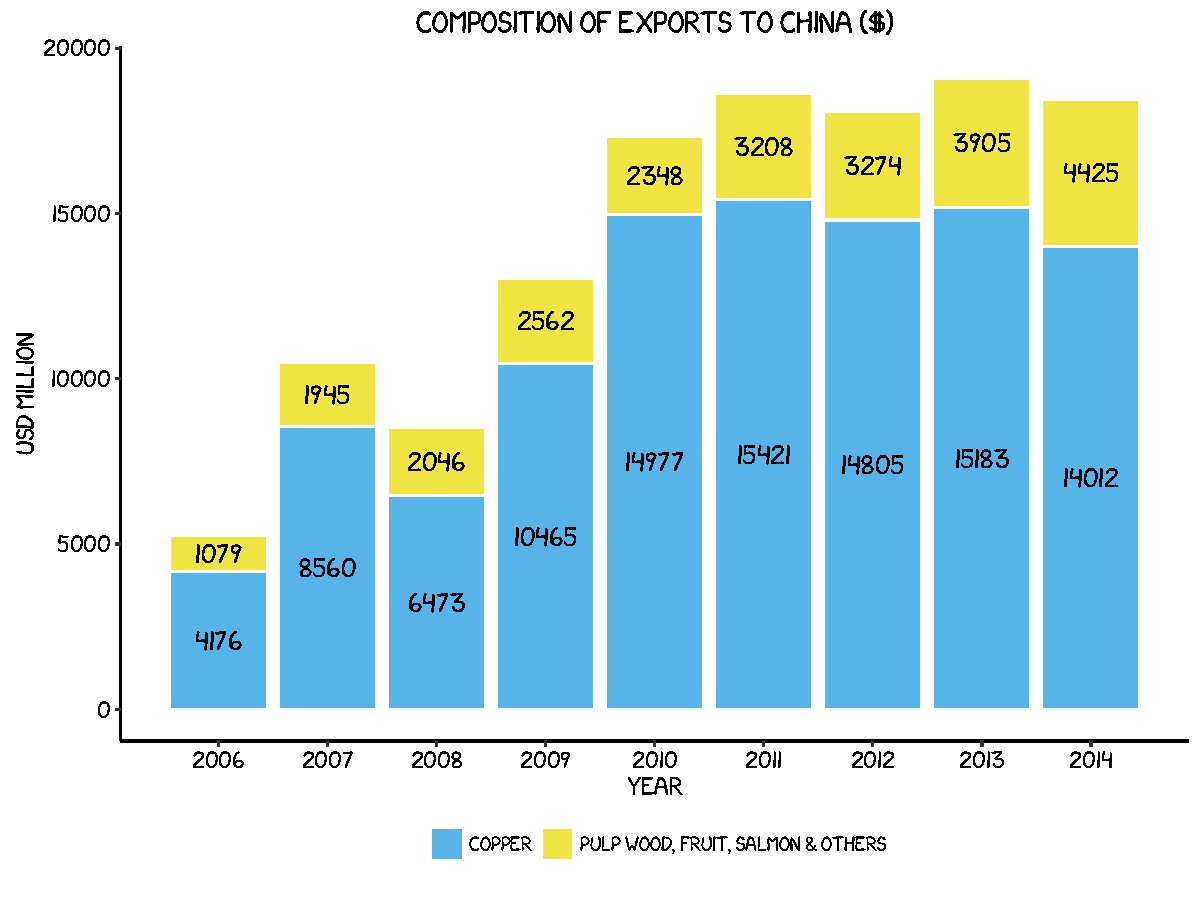
\includegraphics[width=0.55\linewidth]{figures/bar_10-1} \end{center}

\section{\texorpdfstring{Using `The Economist'
theme}{Using The Economist theme}}\label{using-the-economist-theme-2}

There are a wider range of pre-built themes available as part of the
\texttt{ggthemes} package (more information on these
\href{https://cran.r-project.org/web/packages/ggthemes/vignettes/ggthemes.html}{here}).
Below we've applied \texttt{theme\_economist()}, which approximates
graphs in the Economist magazine. It is also important that the font
change argument inside \texttt{theme} is optional and it's only to
obtain a more similar result compared to the original. For an exact
result you need `Officina Sans' which is a commercial font and is
available \href{http://www.myfonts.com/fonts/itc/officina-sans/}{here}.

\begin{Shaded}
\begin{Highlighting}[]
\NormalTok{p3 <-}\StringTok{ }\KeywordTok{ggplot}\NormalTok{() +}
\StringTok{      }\KeywordTok{geom_bar}\NormalTok{(}\KeywordTok{aes}\NormalTok{(}\DataTypeTok{y =} \NormalTok{export, }\DataTypeTok{x =} \NormalTok{year, }\DataTypeTok{fill =} \NormalTok{product), }\DataTypeTok{data =} \NormalTok{charts.data, }
\StringTok{        }\DataTypeTok{stat=}\StringTok{"identity"}\NormalTok{) +}\StringTok{ }
\StringTok{      }\KeywordTok{geom_text}\NormalTok{(}\DataTypeTok{data=}\NormalTok{charts.data, }\KeywordTok{aes}\NormalTok{(}\DataTypeTok{x =} \NormalTok{year, }\DataTypeTok{y =} \NormalTok{pos, }\DataTypeTok{label =} \NormalTok{export), }
\StringTok{        }\DataTypeTok{colour=}\StringTok{"white"}\NormalTok{, }\DataTypeTok{size =} \DecValTok{4}\NormalTok{,}\DataTypeTok{family =} \StringTok{"OfficinaSanITC-Book"}\NormalTok{, }
\StringTok{        }\DataTypeTok{show.legend =} \NormalTok{F) +}\StringTok{ }
\StringTok{      }\KeywordTok{scale_x_continuous}\NormalTok{(}\DataTypeTok{breaks=}\KeywordTok{seq}\NormalTok{(}\DecValTok{2006}\NormalTok{,}\DecValTok{2014}\NormalTok{,}\DecValTok{1}\NormalTok{)) +}\StringTok{ }
\StringTok{      }\KeywordTok{labs}\NormalTok{(}\DataTypeTok{x=}\StringTok{"Year"}\NormalTok{, }\DataTypeTok{y=}\StringTok{"USD million"}\NormalTok{) +}\StringTok{ }
\StringTok{      }\KeywordTok{ggtitle}\NormalTok{(}\StringTok{"Composition of Exports to China ($)"}\NormalTok{) +}
\StringTok{      }\KeywordTok{theme_economist}\NormalTok{() +}\StringTok{ }\KeywordTok{scale_fill_economist}\NormalTok{() +}
\StringTok{      }\KeywordTok{theme}\NormalTok{(}\DataTypeTok{axis.line.x =} \KeywordTok{element_line}\NormalTok{(}\DataTypeTok{size=}\NormalTok{.}\DecValTok{5}\NormalTok{, }\DataTypeTok{colour =} \StringTok{"black"}\NormalTok{), }
        \DataTypeTok{axis.line.y =} \KeywordTok{element_line}\NormalTok{(}\DataTypeTok{size=}\NormalTok{.}\DecValTok{5}\NormalTok{, }\DataTypeTok{colour =} \StringTok{"black"}\NormalTok{),}
        \DataTypeTok{legend.position=}\StringTok{"bottom"}\NormalTok{, }
        \DataTypeTok{legend.direction=}\StringTok{"horizontal"}\NormalTok{, }
        \DataTypeTok{legend.title =} \KeywordTok{element_blank}\NormalTok{(),}
        \DataTypeTok{plot.title=}\KeywordTok{element_text}\NormalTok{(}\DataTypeTok{family=}\StringTok{"OfficinaSanITC-Book"}\NormalTok{),}
        \DataTypeTok{text=}\KeywordTok{element_text}\NormalTok{(}\DataTypeTok{family=}\StringTok{"OfficinaSanITC-Book"}\NormalTok{))   }
\NormalTok{p3}
\end{Highlighting}
\end{Shaded}

\begin{center}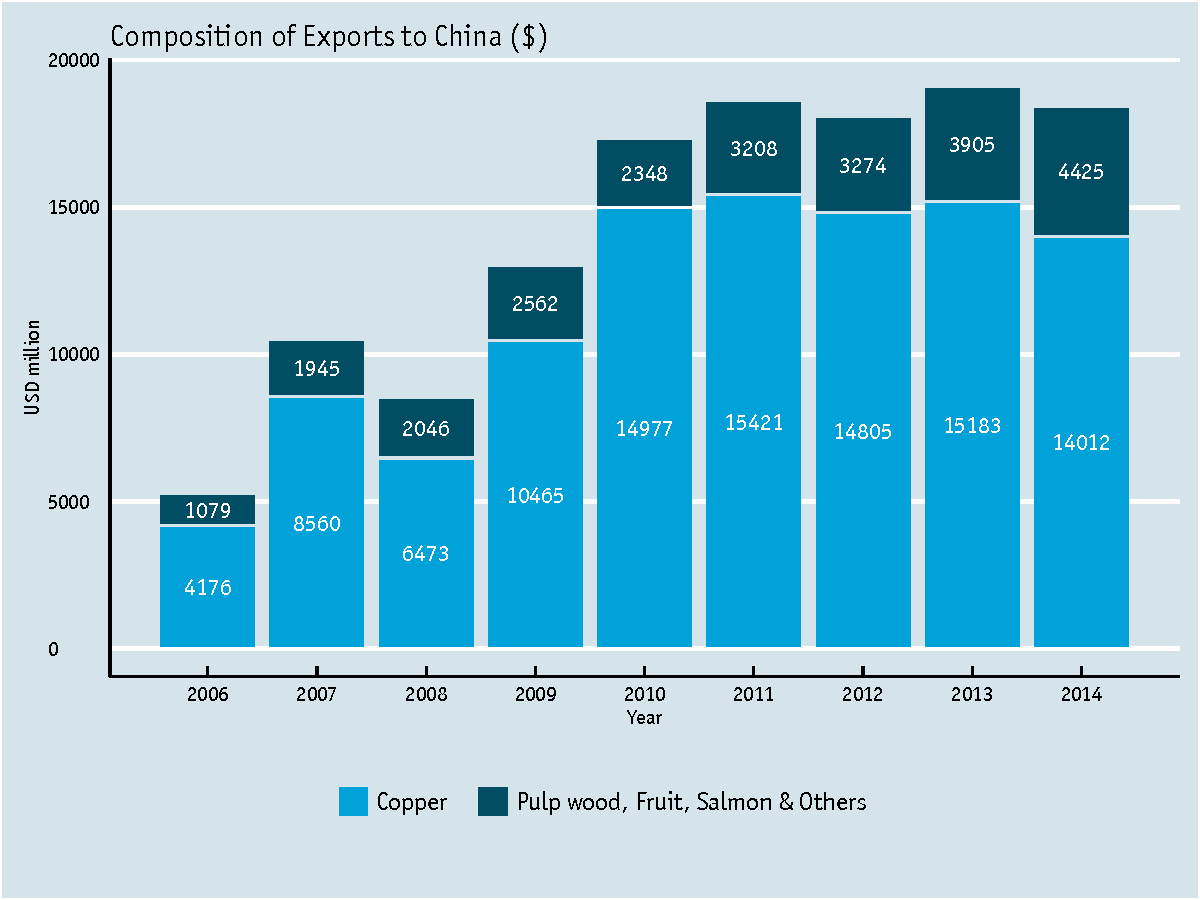
\includegraphics[width=0.55\linewidth]{figures/bar_11-1} \end{center}

\section{Creating your own theme}\label{creating-your-own-theme-2}

As before, you can modify your plots a lot as \texttt{ggplot2} allows
many customisations. Here we present our original result shown at the
top of page.

\begin{Shaded}
\begin{Highlighting}[]
\NormalTok{fill <-}\StringTok{ }\KeywordTok{c}\NormalTok{(}\StringTok{"#40b8d0"}\NormalTok{, }\StringTok{"#b2d183"}\NormalTok{)}

\NormalTok{p3 <-}\StringTok{ }\KeywordTok{ggplot}\NormalTok{() +}\StringTok{ }
\StringTok{      }\KeywordTok{geom_bar}\NormalTok{(}\KeywordTok{aes}\NormalTok{(}\DataTypeTok{y =} \NormalTok{export, }\DataTypeTok{x =} \NormalTok{year, }\DataTypeTok{fill =} \NormalTok{product), }\DataTypeTok{data =} \NormalTok{charts.data, }
\StringTok{        }\DataTypeTok{stat=}\StringTok{"identity"}\NormalTok{) +}\StringTok{ }
\StringTok{      }\KeywordTok{geom_text}\NormalTok{(}\DataTypeTok{data=}\NormalTok{charts.data, }\KeywordTok{aes}\NormalTok{(}\DataTypeTok{x =} \NormalTok{year, }\DataTypeTok{y =} \NormalTok{pos, }\DataTypeTok{label =} \NormalTok{export), }
\StringTok{        }\DataTypeTok{colour=}\StringTok{"black"}\NormalTok{, }\DataTypeTok{family=}\StringTok{"Tahoma"}\NormalTok{, }\DataTypeTok{size =} \DecValTok{4}\NormalTok{, }\DataTypeTok{show.legend =} \NormalTok{F) +}\StringTok{ }
\StringTok{      }\KeywordTok{scale_x_continuous}\NormalTok{(}\DataTypeTok{breaks=}\KeywordTok{seq}\NormalTok{(}\DecValTok{2006}\NormalTok{,}\DecValTok{2014}\NormalTok{,}\DecValTok{1}\NormalTok{)) +}\StringTok{ }
\StringTok{      }\KeywordTok{labs}\NormalTok{(}\DataTypeTok{x=}\StringTok{"Year"}\NormalTok{, }\DataTypeTok{y=}\StringTok{"USD million"}\NormalTok{) +}\StringTok{ }
\StringTok{      }\KeywordTok{ggtitle}\NormalTok{(}\StringTok{"Composition of Exports to China ($)"}\NormalTok{) +}\StringTok{ }
\StringTok{      }\KeywordTok{scale_fill_manual}\NormalTok{(}\DataTypeTok{values=}\NormalTok{fill) +}\StringTok{ }
\StringTok{      }\KeywordTok{theme}\NormalTok{(}\DataTypeTok{axis.line.x =} \KeywordTok{element_line}\NormalTok{(}\DataTypeTok{size=}\NormalTok{.}\DecValTok{5}\NormalTok{, }\DataTypeTok{colour =} \StringTok{"black"}\NormalTok{), }
        \DataTypeTok{axis.line.y =} \KeywordTok{element_line}\NormalTok{(}\DataTypeTok{size=}\NormalTok{.}\DecValTok{5}\NormalTok{, }\DataTypeTok{colour =} \StringTok{"black"}\NormalTok{), }
        \DataTypeTok{axis.text.x=}\KeywordTok{element_text}\NormalTok{(}\DataTypeTok{colour=}\StringTok{"black"}\NormalTok{, }\DataTypeTok{size =} \DecValTok{10}\NormalTok{), }
        \DataTypeTok{axis.text.y=}\KeywordTok{element_text}\NormalTok{(}\DataTypeTok{colour=}\StringTok{"black"}\NormalTok{, }\DataTypeTok{size =} \DecValTok{10}\NormalTok{),}
        \DataTypeTok{legend.key=}\KeywordTok{element_rect}\NormalTok{(}\DataTypeTok{fill=}\StringTok{"white"}\NormalTok{, }\DataTypeTok{colour=}\StringTok{"white"}\NormalTok{),}
        \DataTypeTok{legend.position=}\StringTok{"bottom"}\NormalTok{, }\DataTypeTok{legend.direction=}\StringTok{"horizontal"}\NormalTok{, }
        \DataTypeTok{legend.title =} \KeywordTok{element_blank}\NormalTok{(),}
        \DataTypeTok{panel.grid.major =} \KeywordTok{element_line}\NormalTok{(}\DataTypeTok{colour =} \StringTok{"#d3d3d3"}\NormalTok{), }
        \DataTypeTok{panel.grid.minor =} \KeywordTok{element_blank}\NormalTok{(), }
        \DataTypeTok{panel.border =} \KeywordTok{element_blank}\NormalTok{(), }
        \DataTypeTok{panel.background =} \KeywordTok{element_blank}\NormalTok{(),}
        \DataTypeTok{plot.title =} \KeywordTok{element_text}\NormalTok{(}\DataTypeTok{size =} \DecValTok{14}\NormalTok{, }\DataTypeTok{family =} \StringTok{"Tahoma"}\NormalTok{, }\DataTypeTok{face =} \StringTok{"bold"}\NormalTok{), }
        \DataTypeTok{text=}\KeywordTok{element_text}\NormalTok{(}\DataTypeTok{family=}\StringTok{"Tahoma"}\NormalTok{))  }
\NormalTok{p3}
\end{Highlighting}
\end{Shaded}

\begin{center}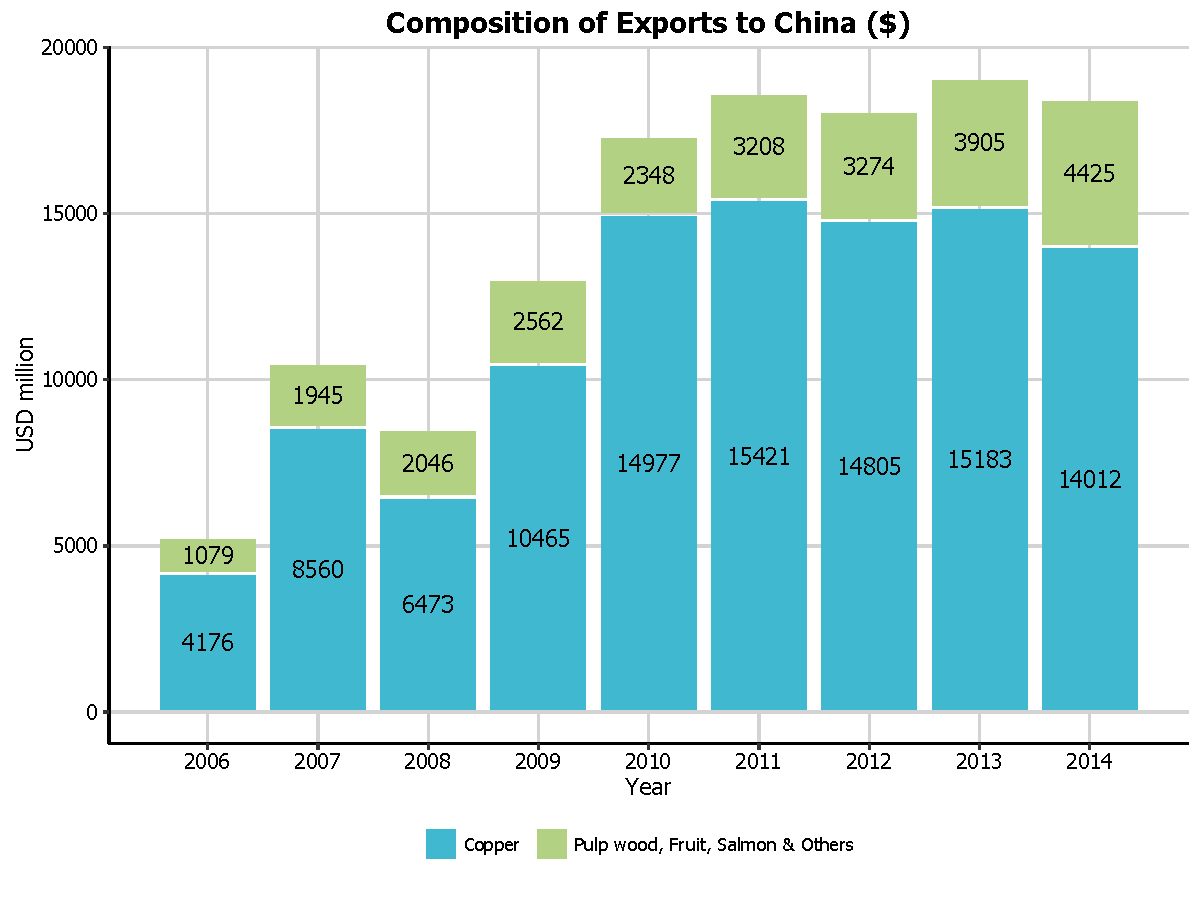
\includegraphics[width=0.55\linewidth]{figures/bar_13-1} \end{center}
\chapter{Stacked Bar Plots}\label{stacked-bar-plots}

In this part, we will work towards creating the bar plot below. We will
take you from a basic stacked bar plot and explain all the
customisations we add to the code step-by-step.

\begin{center}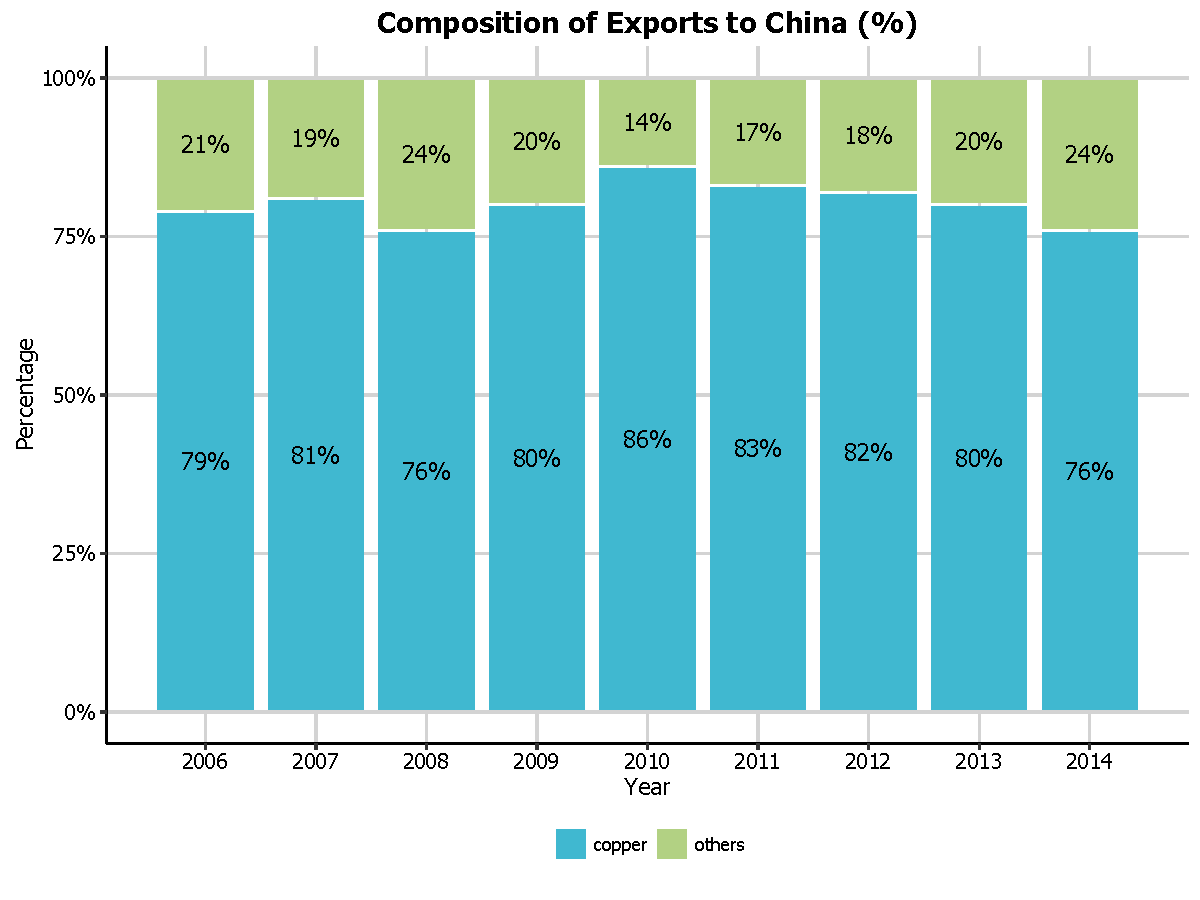
\includegraphics[width=0.55\linewidth]{figures/stacked_finalresult-1} \end{center}

We will use an international trade \href{http://pachamaltese.github.io/stats/trade-chile-china/copper-data-for-tutorial.csv}{dataset} made by ourselves from different sources (Chile Customs,
Central Bank of Chile and General Directorate of International Economic Relations).

\section{Basic graph}\label{basic-graph-3}

In order to initialise a plot we tell ggplot that \texttt{charts.data}
is our data, and specify the variables on each axis. We then instruct
ggplot to render this as a stacked bar plot by adding the
\texttt{geom\_bar} command.

The first thing to do is load in the data and libraries, as below:

\begin{Shaded}
\begin{Highlighting}[]
\KeywordTok{library}\NormalTok{(ggplot2)}
\KeywordTok{library}\NormalTok{(ggthemes)}
\KeywordTok{library}\NormalTok{(extrafont)}
\KeywordTok{library}\NormalTok{(plyr)}
\KeywordTok{library}\NormalTok{(scales)}
\NormalTok{charts.data <-}\StringTok{ }\KeywordTok{read.csv}\NormalTok{(}\StringTok{"copper-data-for-tutorial.csv"}\NormalTok{)}
\end{Highlighting}
\end{Shaded}

\begin{Shaded}
\begin{Highlighting}[]
\NormalTok{charts.data <-}\StringTok{ }\KeywordTok{read.csv}\NormalTok{(}\StringTok{"copper-data-for-tutorial.csv"}\NormalTok{)}

\NormalTok{p4 <-}\StringTok{ }\KeywordTok{ggplot}\NormalTok{() +}\StringTok{ }\KeywordTok{geom_bar}\NormalTok{(}\KeywordTok{aes}\NormalTok{(}\DataTypeTok{y =} \NormalTok{percentage, }\DataTypeTok{x =} \NormalTok{year, }\DataTypeTok{fill =} \NormalTok{product), }
\StringTok{        }\DataTypeTok{data =} \NormalTok{charts.data, }\DataTypeTok{stat=}\StringTok{"identity"}\NormalTok{)}
\NormalTok{p4}
\end{Highlighting}
\end{Shaded}

\begin{center}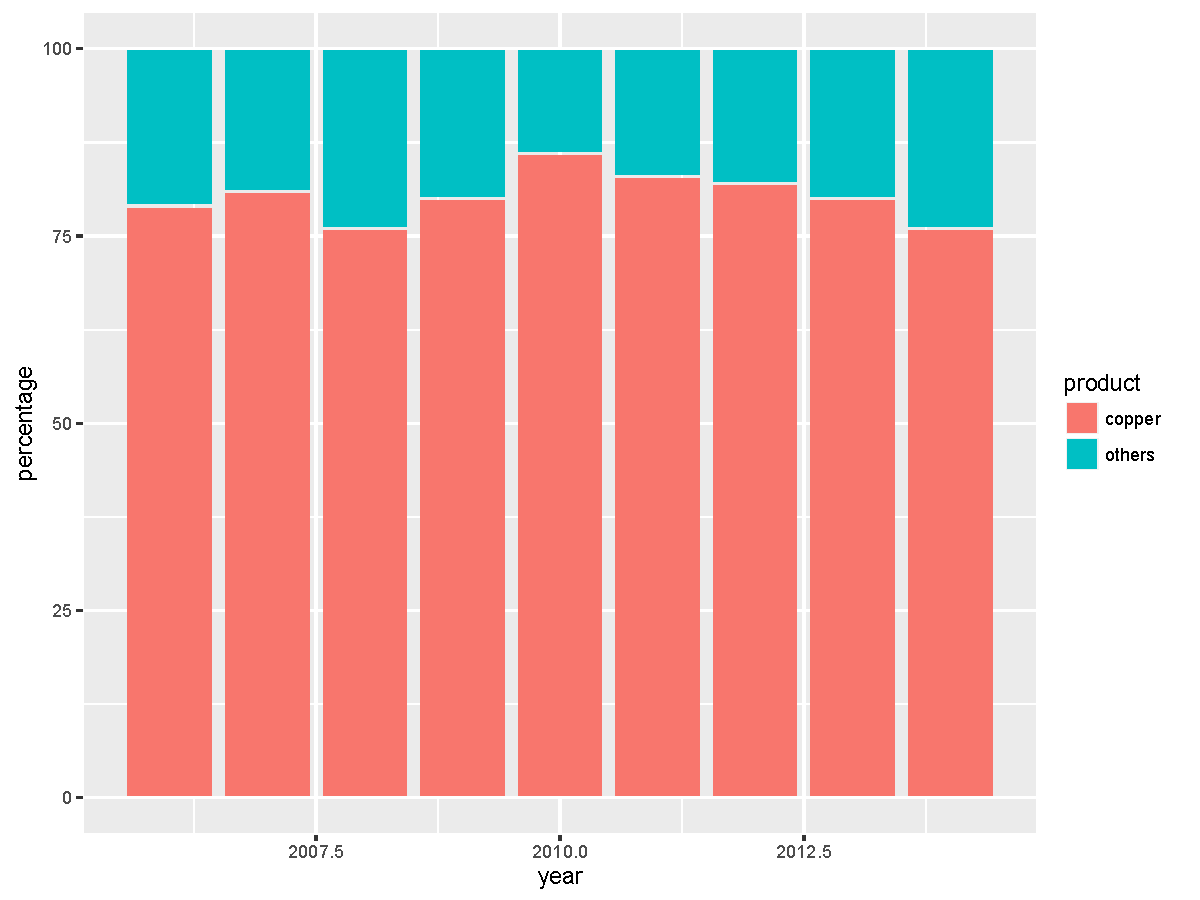
\includegraphics[width=0.55\linewidth]{figures/stacked_1-1} \end{center}

\section{Adding data labels}\label{adding-data-labels-1}

To label the bars according to some variable in the data, we add the
\texttt{label} argument to the \texttt{ggplot(aes())} option. In this
case, we have labelled the bars with numbers from the \texttt{export}
variable.

\begin{Shaded}
\begin{Highlighting}[]
\NormalTok{p4 <-}\StringTok{ }\NormalTok{p4 +}\StringTok{ }\KeywordTok{geom_text}\NormalTok{(}\DataTypeTok{data=}\NormalTok{charts.data, }\KeywordTok{aes}\NormalTok{(}\DataTypeTok{x =} \NormalTok{year, }\DataTypeTok{y =} \NormalTok{percentage, }
\StringTok{        }\DataTypeTok{label =} \KeywordTok{paste0}\NormalTok{(percentage,}\StringTok{"%"}\NormalTok{)), }\DataTypeTok{size=}\DecValTok{4}\NormalTok{)}
\NormalTok{p4}
\end{Highlighting}
\end{Shaded}

\begin{center}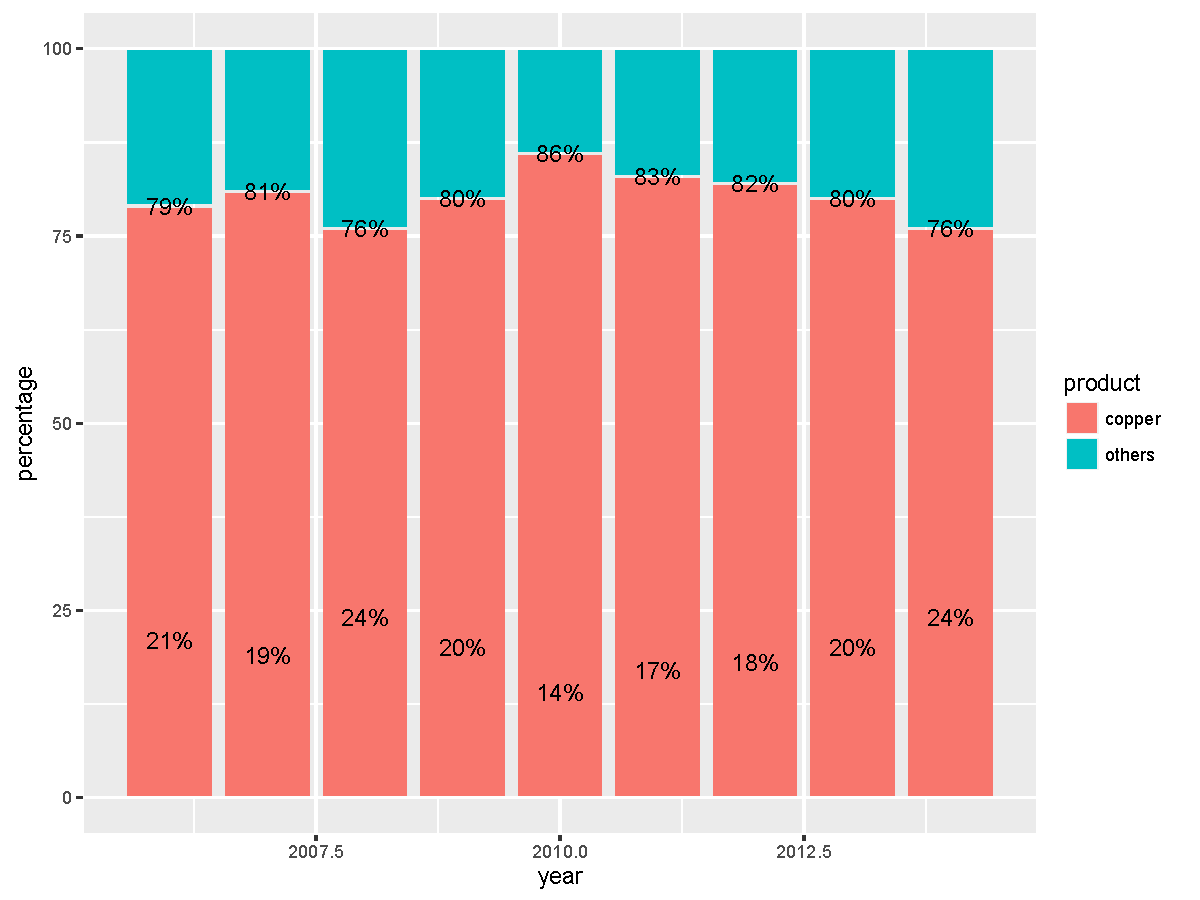
\includegraphics[width=0.55\linewidth]{figures/stacked_2-1} \end{center}

\section{Adjusting data labels
position}\label{adjusting-data-labels-position-1}

To adjust the position of the data labels from the default placement, we
use the \texttt{ddply} function on the data, and create a new variable
called \texttt{pos}. This variable is at the centre of each bar and can
be used to specify the position of the labels by assigning it to the
\texttt{y} argument in \texttt{geom\_text(aes())}.

\begin{Shaded}
\begin{Highlighting}[]
\NormalTok{charts.data <-}\StringTok{ }\KeywordTok{ddply}\NormalTok{(charts.data, .(year), transform, }
\StringTok{        }\DataTypeTok{pos =} \KeywordTok{cumsum}\NormalTok{(percentage) -}\StringTok{ }\NormalTok{(}\FloatTok{0.5} \NormalTok{*}\StringTok{ }\NormalTok{percentage))}

\NormalTok{p4 <-}\StringTok{ }\KeywordTok{ggplot}\NormalTok{() +}\StringTok{ }\KeywordTok{geom_bar}\NormalTok{(}\KeywordTok{aes}\NormalTok{(}\DataTypeTok{y =} \NormalTok{percentage, }\DataTypeTok{x =} \NormalTok{year, }\DataTypeTok{fill =} \NormalTok{product), }
\StringTok{        }\DataTypeTok{data =} \NormalTok{charts.data,}\DataTypeTok{stat=}\StringTok{"identity"}\NormalTok{)}
\NormalTok{p4 <-}\StringTok{ }\NormalTok{p4 +}\StringTok{ }\KeywordTok{geom_text}\NormalTok{(}\DataTypeTok{data=}\NormalTok{charts.data, }\KeywordTok{aes}\NormalTok{(}\DataTypeTok{x =} \NormalTok{year, }\DataTypeTok{y =} \NormalTok{pos, }
\StringTok{        }\DataTypeTok{label =} \KeywordTok{paste0}\NormalTok{(percentage,}\StringTok{"%"}\NormalTok{)),} \DataTypeTok{size=}\DecValTok{4}\NormalTok{)}
\NormalTok{p4}
\end{Highlighting}
\end{Shaded}

\begin{center}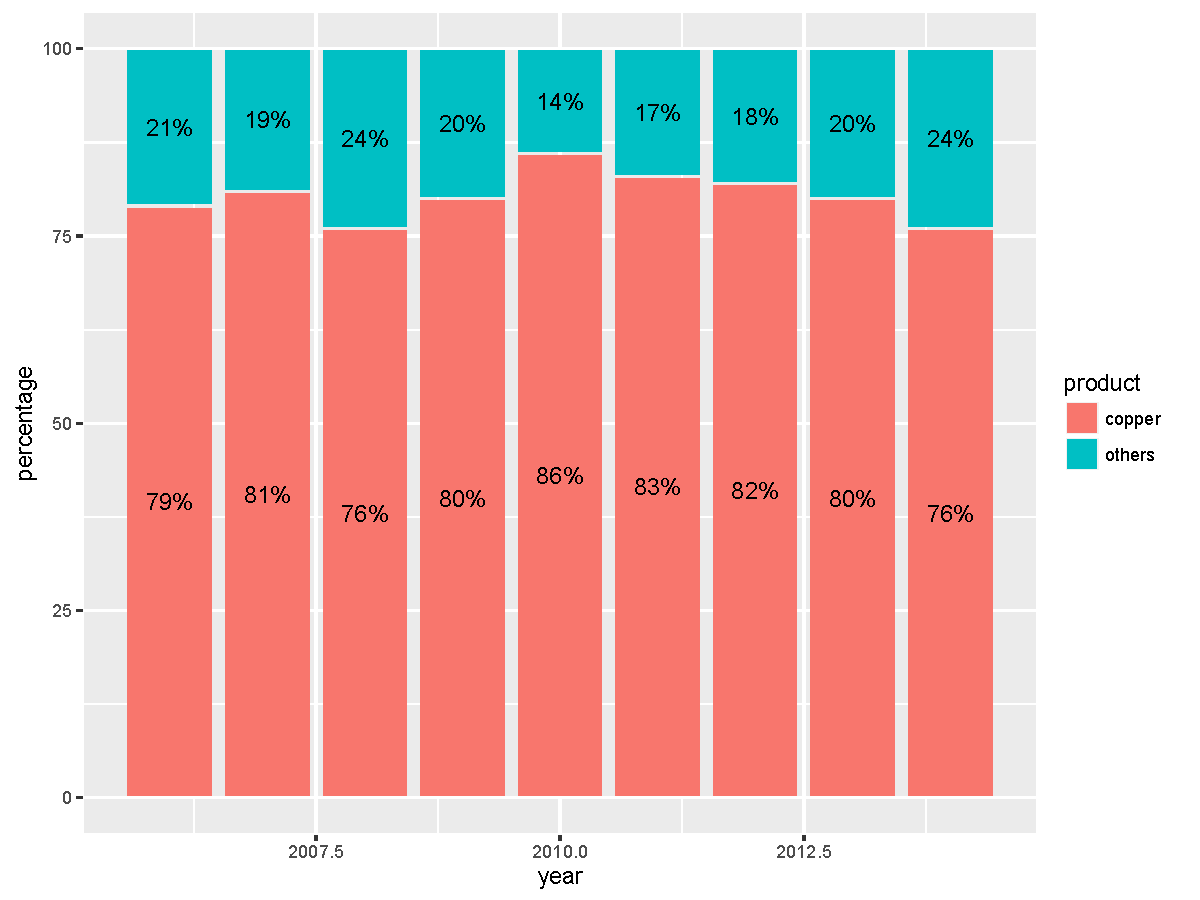
\includegraphics[width=0.55\linewidth]{figures/stacked_3-1} \end{center}

\section{Adjusting legend
position}\label{adjusting-legend-position-2}

To adjust the position of the legend from the default spot of right of
the graph, we add the \texttt{theme} option and specify the
\texttt{legend.position="bottom"} argument. We can also change the title
to blank using the \texttt{legend.title\ =\ element\_blank()} argument
and change the legend shape using the
\texttt{legend.direction="horizontal"} argument.

\begin{Shaded}
\begin{Highlighting}[]
\NormalTok{p4 <-}\StringTok{ }\NormalTok{p4 +}\StringTok{ }\KeywordTok{theme}\NormalTok{(}\DataTypeTok{legend.position=}\StringTok{"bottom"}\NormalTok{, }\DataTypeTok{legend.direction=}\StringTok{"horizontal"}\NormalTok{, }
\StringTok{        }\DataTypeTok{legend.title =} \KeywordTok{element_blank}\NormalTok{())}
\NormalTok{p4}
\end{Highlighting}
\end{Shaded}

\begin{center}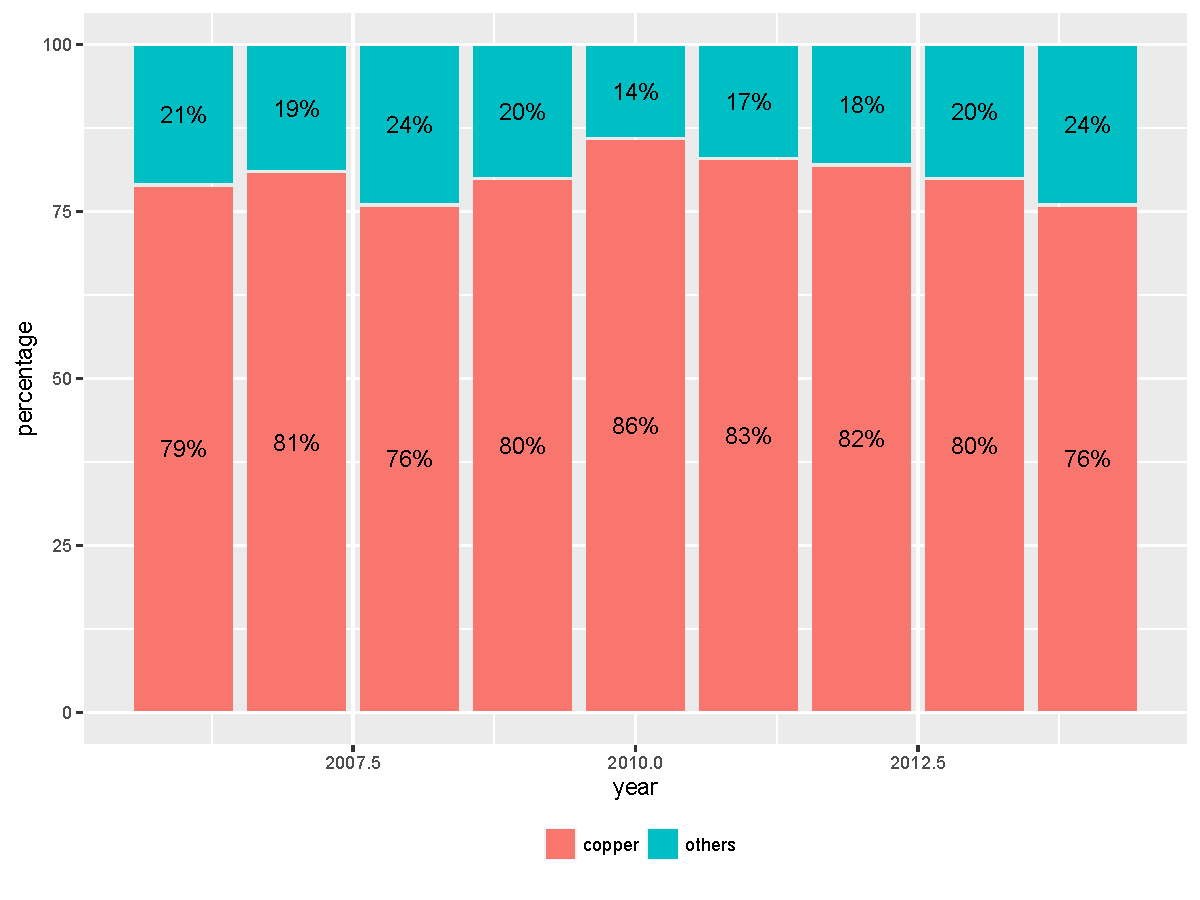
\includegraphics[width=0.55\linewidth]{figures/stacked_4-1} \end{center}

\section{Changing variables
display}\label{changing-variables-display-3}

To change the variables' displayed name, we need to re-factor our data
labels in \texttt{charts.data} data frame.

\begin{Shaded}
\begin{Highlighting}[]
\NormalTok{charts.data <-}\StringTok{ }\KeywordTok{as.data.frame}\NormalTok{(charts.data)}
\NormalTok{charts.data$product <-}\StringTok{ }\KeywordTok{factor}\NormalTok{(charts.data$product, }
\StringTok{        }\DataTypeTok{levels =} \KeywordTok{c}\NormalTok{(}\StringTok{"copper"}\NormalTok{,}\StringTok{"others"}\NormalTok{), }
\StringTok{        }\DataTypeTok{labels =} \KeywordTok{c}\NormalTok{(}\StringTok{"Copper"}\NormalTok{,}\StringTok{"Pulp wood, Fruit, Salmon & Others"}\NormalTok{))}

\NormalTok{p4 <-}\StringTok{ }\KeywordTok{ggplot}\NormalTok{() +}\StringTok{ }
\StringTok{      }\KeywordTok{geom_bar}\NormalTok{(}\KeywordTok{aes}\NormalTok{(}\DataTypeTok{y =} \NormalTok{percentage, }\DataTypeTok{x =} \NormalTok{year, }\DataTypeTok{fill =} \NormalTok{product), }
\StringTok{        }\DataTypeTok{data =} \NormalTok{charts.data, }\DataTypeTok{stat=}\StringTok{"identity"}\NormalTok{) +}\StringTok{ }
\StringTok{      }\KeywordTok{geom_text}\NormalTok{(}\DataTypeTok{data=}\NormalTok{charts.data, }\KeywordTok{aes}\NormalTok{(}\DataTypeTok{x =} \NormalTok{year, }\DataTypeTok{y =} \NormalTok{pos, }
\StringTok{        }\DataTypeTok{label =} \KeywordTok{paste0}\NormalTok{(percentage,}\StringTok{"%"}\NormalTok{)), }\DataTypeTok{size=}\DecValTok{4}\NormalTok{) +}
\StringTok{      }\KeywordTok{theme}\NormalTok{(}\DataTypeTok{legend.position=}\StringTok{"bottom"}\NormalTok{, }\DataTypeTok{legend.direction=}\StringTok{"horizontal"}\NormalTok{, }
\StringTok{        }\DataTypeTok{legend.title =} \KeywordTok{element_blank}\NormalTok{())}
\NormalTok{p4}
\end{Highlighting}
\end{Shaded}

\begin{center}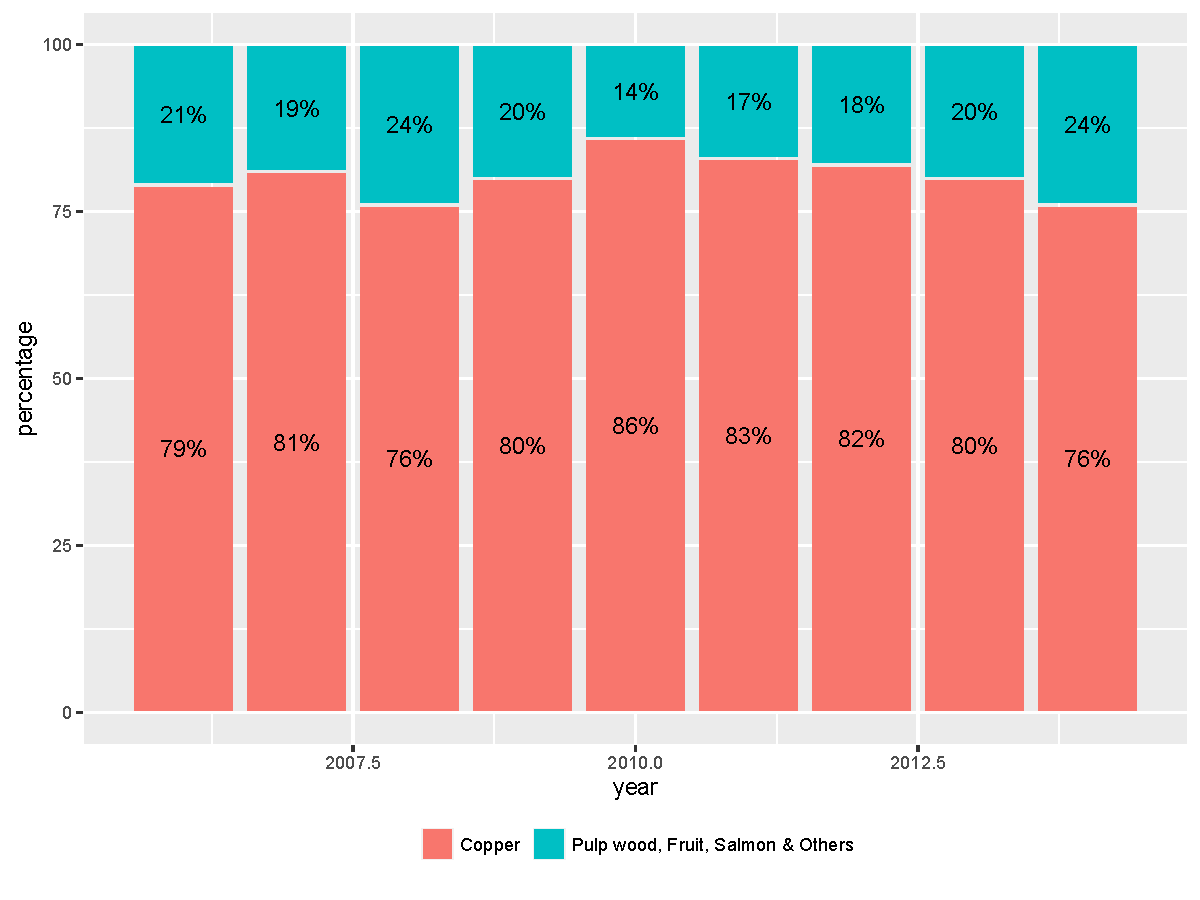
\includegraphics[width=0.55\linewidth]{figures/stacked_5-1} \end{center}

\section{Adjusting x-axis scale}\label{adjusting-x-axis-scale-3}

To change the axis tick marks, we use the \texttt{scale\_x\_continuous}
and/or \texttt{scale\_y\_continuous} commands.

\begin{Shaded}
\begin{Highlighting}[]
\NormalTok{p4 <-}\StringTok{ }\NormalTok{p4 +}\StringTok{ }\KeywordTok{scale_x_continuous}\NormalTok{(}\DataTypeTok{breaks=}\KeywordTok{seq}\NormalTok{(}\DecValTok{2006}\NormalTok{,}\DecValTok{2014}\NormalTok{,}\DecValTok{1}\NormalTok{))}
\NormalTok{p4}
\end{Highlighting}
\end{Shaded}

\begin{center}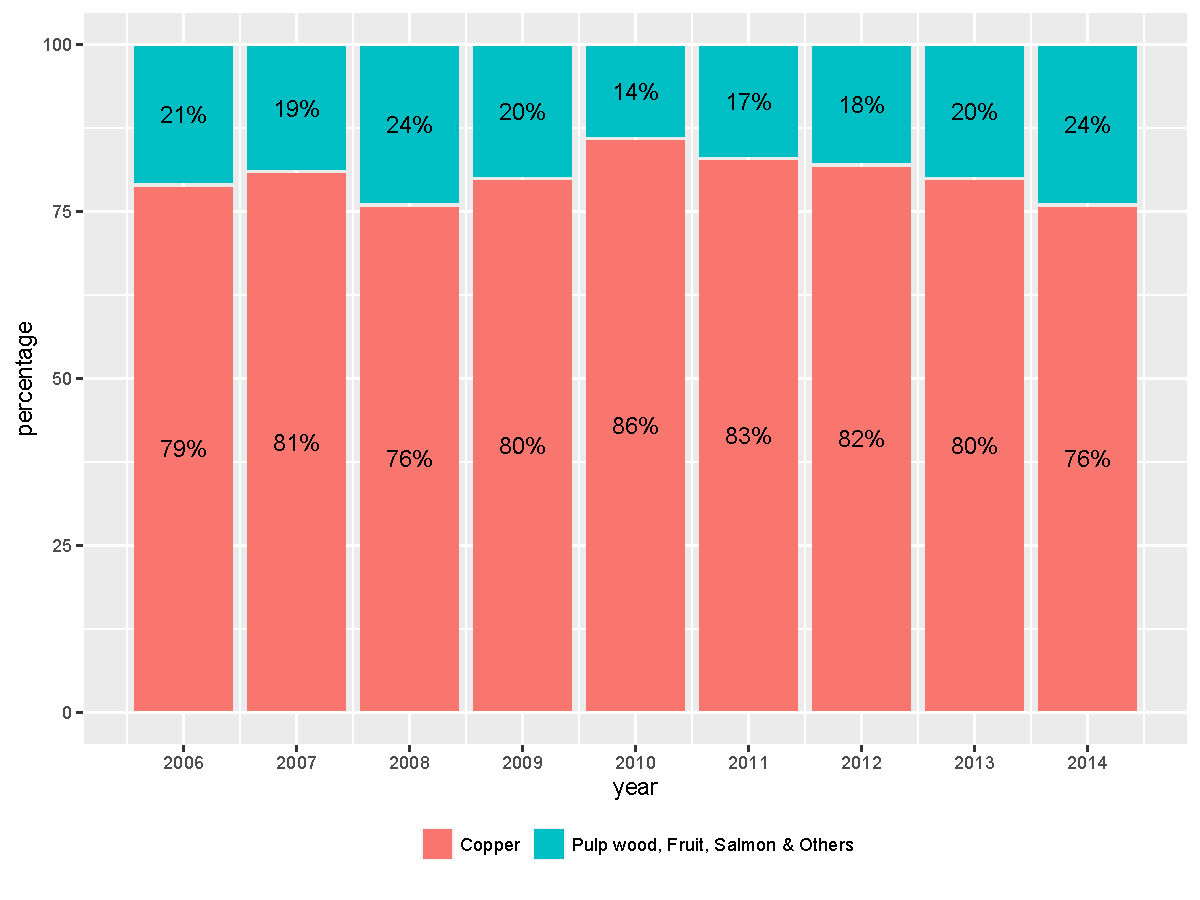
\includegraphics[width=0.55\linewidth]{figures/stacked_6-1} \end{center}

\section{Adjusting axis, title \&
units}\label{adjusting-axis-title-units}

To add a title, we include the option \texttt{ggtitle} and include the
name of the graph as a string argument, and to change the axis names we
use the \texttt{labs} command.

\begin{Shaded}
\begin{Highlighting}[]
\NormalTok{p4 <-}\StringTok{ }\NormalTok{p4 +}\StringTok{ }\KeywordTok{labs}\NormalTok{(}\DataTypeTok{x=}\StringTok{"Year"}\NormalTok{, }\DataTypeTok{y=}\StringTok{"Percentage"}\NormalTok{) +}\StringTok{ }
\StringTok{      }\KeywordTok{scale_y_continuous}\NormalTok{(}\DataTypeTok{labels =} \KeywordTok{dollar_format}\NormalTok{(}\DataTypeTok{suffix =} \StringTok{"%"}\NormalTok{, }\DataTypeTok{prefix =} \StringTok{""}\NormalTok{)) +}
\StringTok{      }\KeywordTok{ggtitle}\NormalTok{(}\StringTok{"Composition of Exports to China (%)"}\NormalTok{) }
\NormalTok{p4}
\end{Highlighting}
\end{Shaded}

\begin{center}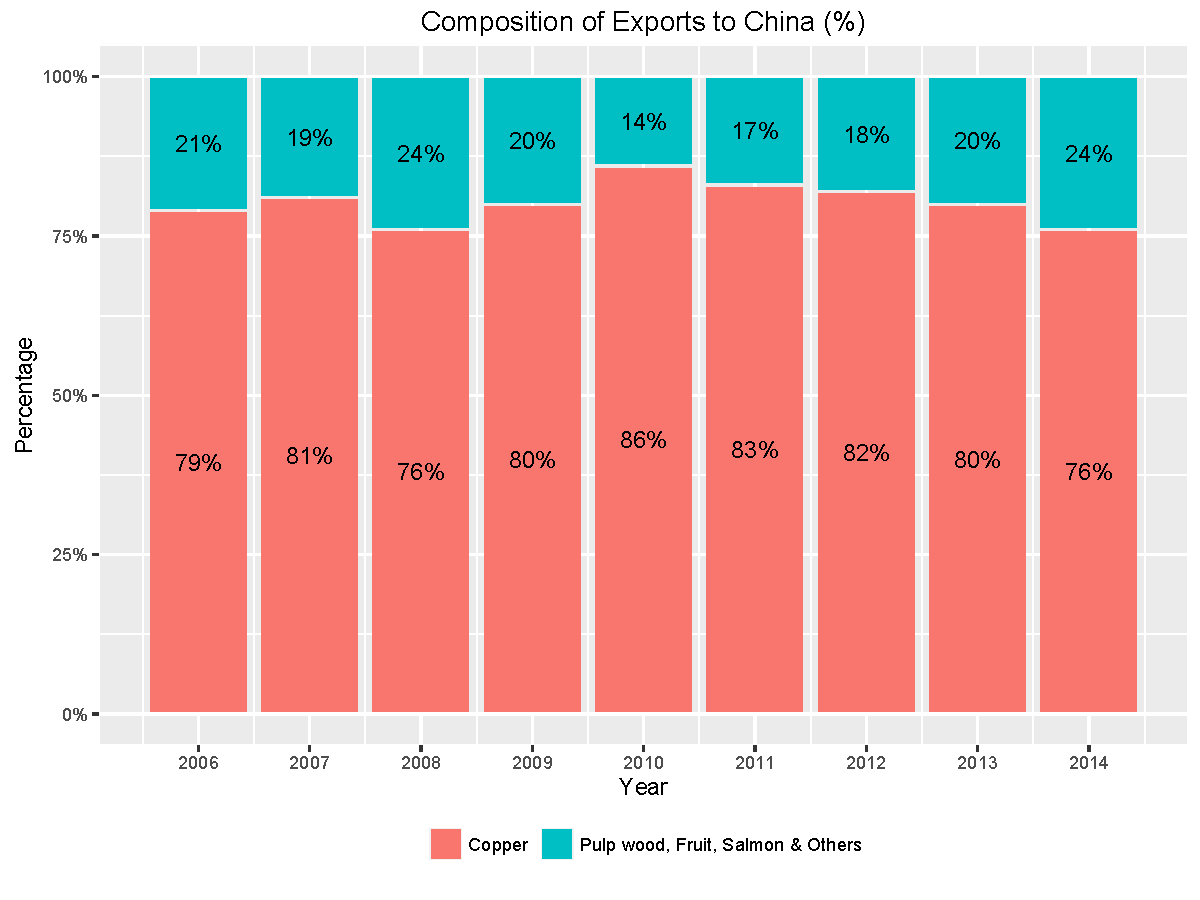
\includegraphics[width=0.55\linewidth]{figures/stacked_7-1} \end{center}

\section{Adjusting color palette}\label{adjusting-color-palette-3}

To change the colours, we use the \texttt{scale\_colour\_manual}
command. Note that you can reference the specific colours you'd like to
use with specific HEX codes. You can also reference colours by name,
with the full list of colours recognised by R
\href{http://www.stat.columbia.edu/~tzheng/files/Rcolor.pdf}{here}.

\begin{Shaded}
\begin{Highlighting}[]
\NormalTok{fill <-}\StringTok{ }\KeywordTok{c}\NormalTok{(}\StringTok{"#5F9EA0"}\NormalTok{, }\StringTok{"#E1B378"}\NormalTok{)}
\NormalTok{p4 <-}\StringTok{ }\NormalTok{p4 +}\StringTok{ }\KeywordTok{scale_fill_manual}\NormalTok{(}\DataTypeTok{values=}\NormalTok{fill)}
\NormalTok{p4}
\end{Highlighting}
\end{Shaded}

\begin{center}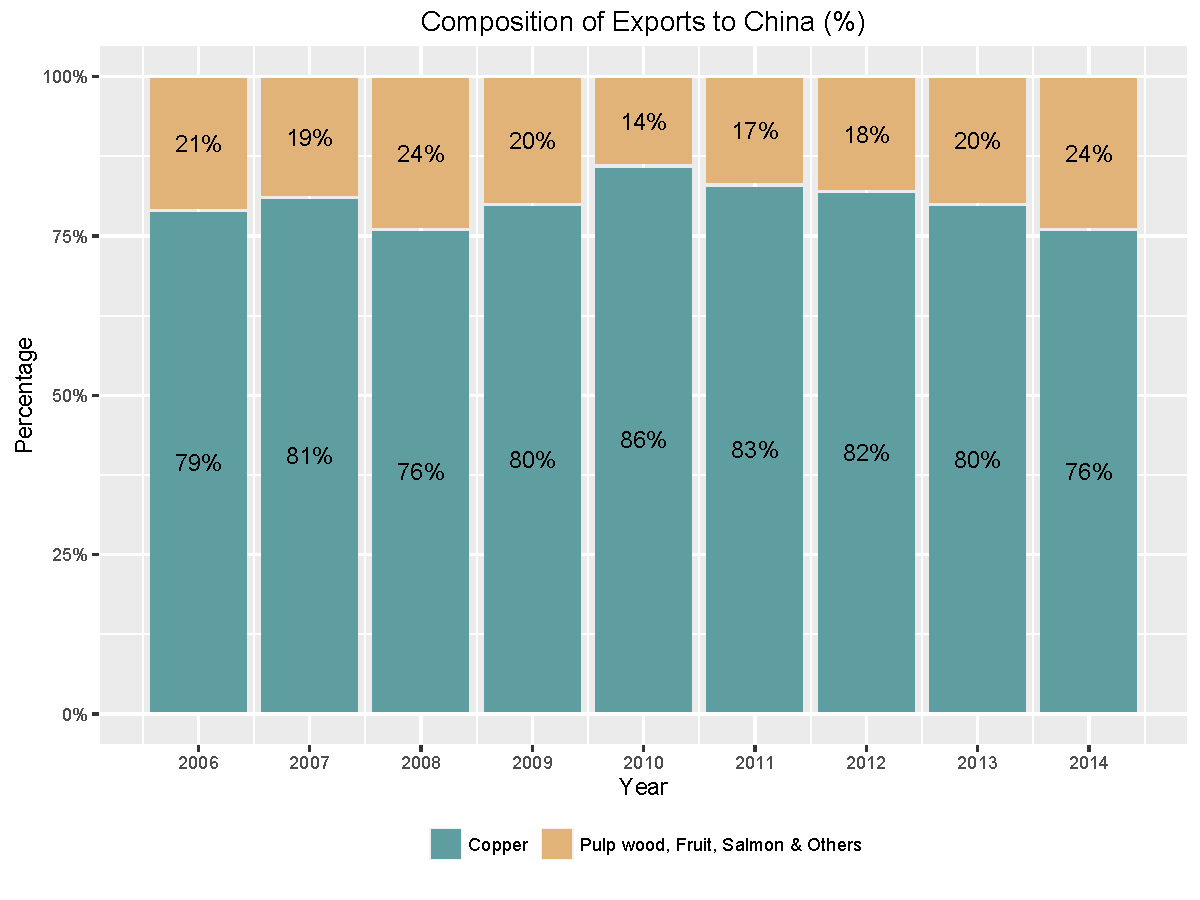
\includegraphics[width=0.55\linewidth]{figures/stacked_8-1} \end{center}

\section{Using the white theme}\label{using-the-white-theme-3}

As explained in the previous posts, we can also change the overall look
of the graph using themes. We'll start using a simple theme
customisation by adding \texttt{theme\_bw()} after \texttt{ggplot()}. As
you can see, we can further tweak the graph using the \texttt{theme}
option, which we've used so far to change the legend.

\begin{Shaded}
\begin{Highlighting}[]
\NormalTok{p4 <-}\StringTok{ }\KeywordTok{ggplot}\NormalTok{() +}\StringTok{ }
\StringTok{      }\KeywordTok{geom_bar}\NormalTok{(}\KeywordTok{aes}\NormalTok{(}\DataTypeTok{y =} \NormalTok{percentage, }\DataTypeTok{x =} \NormalTok{year, }\DataTypeTok{fill =} \NormalTok{product), }
\StringTok{        }\DataTypeTok{data =} \NormalTok{charts.data, }\DataTypeTok{stat=}\StringTok{"identity"}\NormalTok{) +}\StringTok{ }
\StringTok{      }\KeywordTok{geom_text}\NormalTok{(}\DataTypeTok{data=}\NormalTok{charts.data, }\KeywordTok{aes}\NormalTok{(}\DataTypeTok{x =} \NormalTok{year, }\DataTypeTok{y =} \NormalTok{pos, }
\StringTok{        }\DataTypeTok{label =} \KeywordTok{paste0}\NormalTok{(percentage,}\StringTok{"%"}\NormalTok{)), }\DataTypeTok{size=}\DecValTok{4}\NormalTok{) +}\StringTok{ }
\StringTok{      }\KeywordTok{scale_x_continuous}\NormalTok{(}\DataTypeTok{breaks=}\KeywordTok{seq}\NormalTok{(}\DecValTok{2006}\NormalTok{,}\DecValTok{2014}\NormalTok{,}\DecValTok{1}\NormalTok{)) +}\StringTok{ }
\StringTok{      }\KeywordTok{scale_y_continuous}\NormalTok{(}\DataTypeTok{labels =} \KeywordTok{dollar_format}\NormalTok{(}\DataTypeTok{suffix =} \StringTok{"%"}\NormalTok{, }\DataTypeTok{prefix =} \StringTok{""}\NormalTok{)) +}\StringTok{ }
\StringTok{      }\KeywordTok{labs}\NormalTok{(}\DataTypeTok{x=}\StringTok{"Year"}\NormalTok{, }\DataTypeTok{y=}\StringTok{"Percentage"}\NormalTok{) +}\StringTok{ }
\StringTok{      }\KeywordTok{ggtitle}\NormalTok{(}\StringTok{"Composition of Exports to China (%)"}\NormalTok{) +}
\StringTok{      }\KeywordTok{theme_bw}\NormalTok{() +}
\StringTok{      }\KeywordTok{theme}\NormalTok{(}\DataTypeTok{legend.position=}\StringTok{"bottom"}\NormalTok{, }
\StringTok{        }\DataTypeTok{legend.direction=}\StringTok{"horizontal"}\NormalTok{, }
\StringTok{        }\DataTypeTok{legend.title =} \KeywordTok{element_blank}\NormalTok{())    }
\NormalTok{p4}
\end{Highlighting}
\end{Shaded}

\begin{center}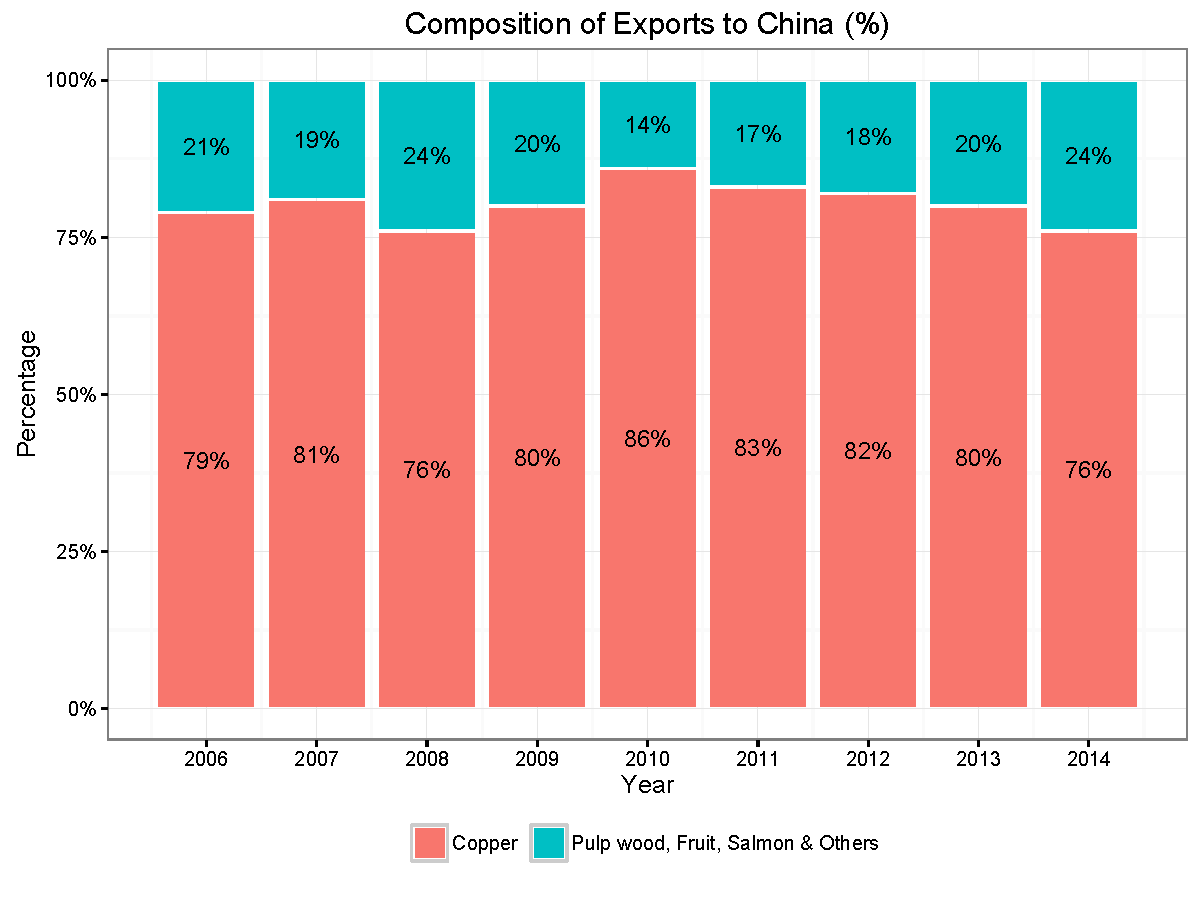
\includegraphics[width=0.55\linewidth]{figures/stacked_9-1} \end{center}

\section{Creating an XKCD style
chart}\label{creating-an-xkcd-style-chart-3}

Of course, you may want to create your own themes as well.
\texttt{ggplot2} allows for a very high degree of customisation,
including allowing you to use imported fonts. Below is an example of a
theme Mauricio was able to create which mimics the visual style of
\href{http://xkcd.com/}{XKCD}. In order to create this chart, you first
need to import the XKCD font, install it on your machine and load it
into R using the \texttt{extrafont} package. These instructions are
taken from
\href{https://www.google.com.au/url?sa=t\&rct=j\&q=\&esrc=s\&source=web\&cd=1\&ved=0ahUKEwiWzafchdPJAhVBpJQKHe_LDT8QFggbMAA\&url=https\%3A\%2F\%2Fcran.r-project.org\%2Fweb\%2Fpackages\%2Fxkcd\%2Fvignettes\%2Fxkcd-intro.pdf\&usg=AFQjCNE-KciGY14e-Q1buYIVmTFC0ht__Q\&sig2=DZUwkvIHwfNWtTtkcz94jg}{here}:

\begin{Shaded}
\begin{Highlighting}[]
\KeywordTok{library}\NormalTok{(extrafont)}

\KeywordTok{download.file}\NormalTok{(}\StringTok{"http://simonsoftware.se/other/xkcd.ttf"}\NormalTok{, }
\StringTok{      }\DataTypeTok{dest=}\StringTok{"xkcd.ttf"}\NormalTok{, }\DataTypeTok{mode=}\StringTok{"wb"}\NormalTok{)}
\KeywordTok{system}\NormalTok{(}\StringTok{"mkdir ~/.fonts"}\NormalTok{)}
\KeywordTok{system}\NormalTok{(}\StringTok{"cp xkcd.ttf  ~/.fonts"}\NormalTok{)}
\KeywordTok{font_import}\NormalTok{(}\DataTypeTok{paths =} \StringTok{"~/.fonts"}\NormalTok{, }\DataTypeTok{pattern=}\StringTok{"[X/x]kcd"}\NormalTok{)}
\KeywordTok{fonts}\NormalTok{()}
\KeywordTok{loadfonts}\NormalTok{()}
\end{Highlighting}
\end{Shaded}

You can then create your graph:

\begin{Shaded}
\begin{Highlighting}[]
\CommentTok{#font_import(pattern="[X/x]kcd")}
\CommentTok{#fonts()}

\NormalTok{fill <-}\StringTok{ }\KeywordTok{c}\NormalTok{(}\StringTok{"#56B4E9"}\NormalTok{, }\StringTok{"#F0E442"}\NormalTok{)}

\NormalTok{p4 <-}\StringTok{ }\KeywordTok{ggplot}\NormalTok{() +}\StringTok{ }
\StringTok{      }\KeywordTok{geom_bar}\NormalTok{(}\KeywordTok{aes}\NormalTok{(}\DataTypeTok{y =} \NormalTok{percentage, }\DataTypeTok{x =} \NormalTok{year, }\DataTypeTok{fill =} \NormalTok{product), }
\StringTok{        }\DataTypeTok{data =} \NormalTok{charts.data, }\DataTypeTok{stat=}\StringTok{"identity"}\NormalTok{) +}\StringTok{ }
\StringTok{      }\KeywordTok{geom_text}\NormalTok{(}\DataTypeTok{data=}\NormalTok{charts.data, }\KeywordTok{aes}\NormalTok{(}\DataTypeTok{x =} \NormalTok{year, }\DataTypeTok{y =} \NormalTok{pos, }
\StringTok{        }\DataTypeTok{label =} \KeywordTok{paste0}\NormalTok{(percentage,}\StringTok{"%"}\NormalTok{)), }
\StringTok{        }\DataTypeTok{colour=}\StringTok{"black"}\NormalTok{, }\DataTypeTok{family=}\StringTok{"xkcd-Regular"}\NormalTok{, }\DataTypeTok{size =} \DecValTok{5}\NormalTok{, }\DataTypeTok{show.legend =} \NormalTok{F) +}\StringTok{ }
\StringTok{      }\KeywordTok{scale_x_continuous}\NormalTok{(}\DataTypeTok{breaks=}\KeywordTok{seq}\NormalTok{(}\DecValTok{2006}\NormalTok{,}\DecValTok{2014}\NormalTok{,}\DecValTok{1}\NormalTok{)) +}\StringTok{ }
\StringTok{      }\KeywordTok{scale_y_continuous}\NormalTok{(}\DataTypeTok{labels =} \KeywordTok{dollar_format}\NormalTok{(}\DataTypeTok{suffix =} \StringTok{"%"}\NormalTok{, }\DataTypeTok{prefix =} \StringTok{""}\NormalTok{)) +}\StringTok{ }
\StringTok{      }\KeywordTok{labs}\NormalTok{(}\DataTypeTok{x=}\StringTok{"Year"}\NormalTok{, }\DataTypeTok{y=}\StringTok{"Percentage"}\NormalTok{) +}\StringTok{ }
\StringTok{      }\KeywordTok{ggtitle}\NormalTok{(}\StringTok{"Composition of Exports to China (%)"}\NormalTok{) +}\StringTok{ }
\StringTok{      }\KeywordTok{scale_fill_manual}\NormalTok{(}\DataTypeTok{values=}\NormalTok{fill) +}\StringTok{ }
\StringTok{      }\KeywordTok{theme}\NormalTok{(}\DataTypeTok{axis.text.x=}\KeywordTok{element_text}\NormalTok{(}\DataTypeTok{colour=}\StringTok{"black"}\NormalTok{, }\DataTypeTok{size =} \DecValTok{10}\NormalTok{), }
\StringTok{        }\DataTypeTok{axis.text.y=}\KeywordTok{element_text}\NormalTok{(}\DataTypeTok{colour=}\StringTok{"black"}\NormalTok{, }\DataTypeTok{size =} \DecValTok{10}\NormalTok{),}
\StringTok{        }\DataTypeTok{axis.line.x =} \KeywordTok{element_line}\NormalTok{(}\DataTypeTok{size=}\NormalTok{.}\DecValTok{5}\NormalTok{, }\DataTypeTok{colour =} \StringTok{"black"}\NormalTok{),}
\StringTok{        }\DataTypeTok{axis.line.y =} \KeywordTok{element_line}\NormalTok{(}\DataTypeTok{size=}\NormalTok{.}\DecValTok{5}\NormalTok{, }\DataTypeTok{colour =} \StringTok{"black"}\NormalTok{),}
\StringTok{        }\DataTypeTok{legend.key=}\KeywordTok{element_rect}\NormalTok{(}\DataTypeTok{fill=}\StringTok{"white"}\NormalTok{, }\DataTypeTok{colour=}\StringTok{"white"}\NormalTok{),}
\StringTok{        }\DataTypeTok{legend.position=}\StringTok{"bottom"}\NormalTok{, }\DataTypeTok{legend.direction=}\StringTok{"horizontal"}\NormalTok{, }
\StringTok{        }\DataTypeTok{legend.title =} \KeywordTok{element_blank}\NormalTok{(),}
\StringTok{        }\DataTypeTok{panel.grid.major =} \KeywordTok{element_blank}\NormalTok{(),}
\StringTok{        }\DataTypeTok{panel.grid.minor =} \KeywordTok{element_blank}\NormalTok{(), }\DataTypeTok{panel.border =} \KeywordTok{element_blank}\NormalTok{(), }
\StringTok{        }\DataTypeTok{panel.background =} \KeywordTok{element_blank}\NormalTok{(),}
\StringTok{        }\DataTypeTok{plot.title=}\KeywordTok{element_text}\NormalTok{(}\DataTypeTok{family=}\StringTok{"xkcd-Regular"}\NormalTok{), }
\StringTok{        }\DataTypeTok{text=}\KeywordTok{element_text}\NormalTok{(}\DataTypeTok{family=}\StringTok{"xkcd-Regular"}\NormalTok{)) }
\NormalTok{p4}
\end{Highlighting}
\end{Shaded}

\begin{center}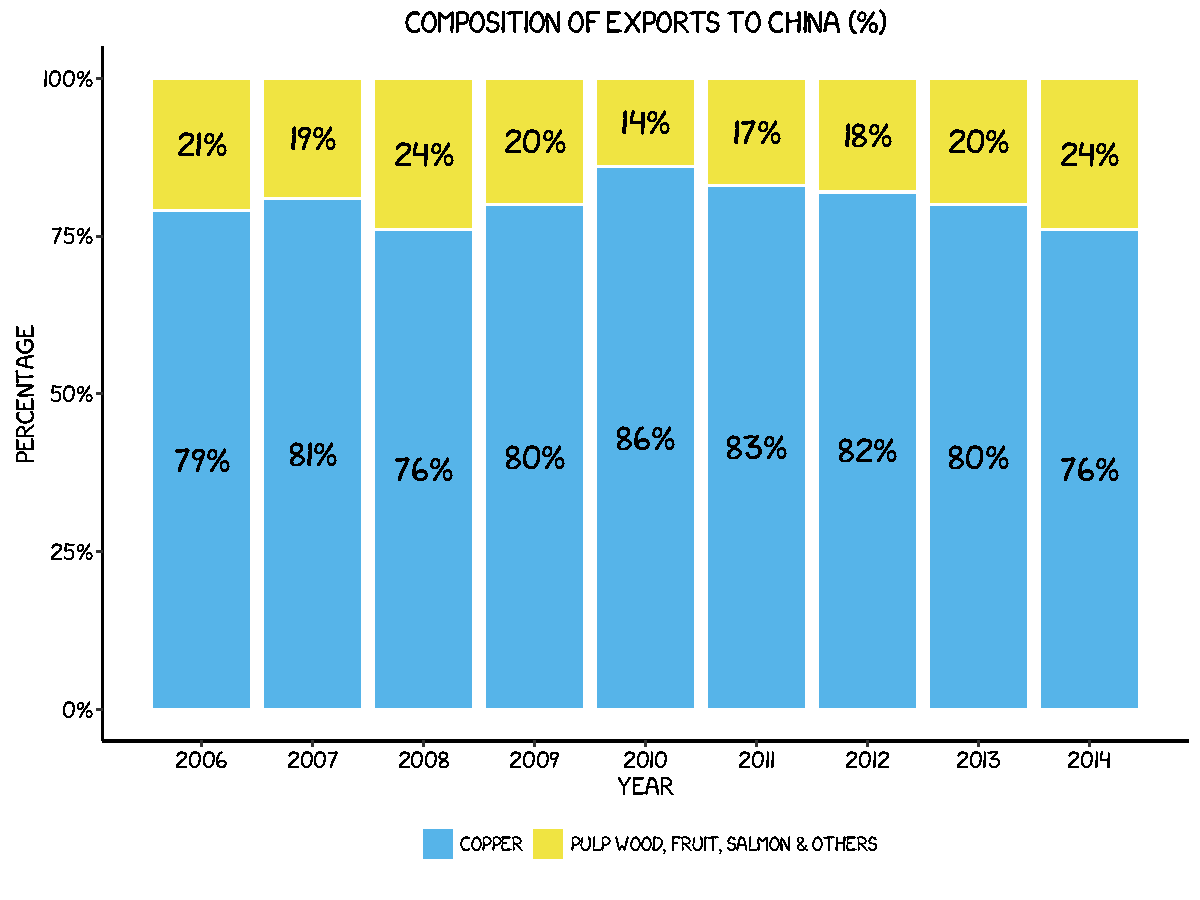
\includegraphics[width=0.55\linewidth]{figures/stacked_10-1} \end{center}

\section{\texorpdfstring{Using `The Economist'
theme}{Using The Economist theme}}\label{using-the-economist-theme-3}

There are a wider range of pre-built themes available as part of the
\texttt{ggthemes} package (more information on these
\href{https://cran.r-project.org/web/packages/ggthemes/vignettes/ggthemes.html}{here}).
Below we've applied \texttt{theme\_economist()}, which approximates
graphs in the Economist magazine. It is also important that the font
change argument inside \texttt{theme} is optional and it's only to
obtain a more similar result compared to the original. For an exact
result you need `Officina Sans' which is a commercial font and is
available \href{http://www.myfonts.com/fonts/itc/officina-sans/}{here}.

\begin{Shaded}
\begin{Highlighting}[]
\NormalTok{p4 <-}\StringTok{ }\KeywordTok{ggplot}\NormalTok{() +}
\StringTok{      }\KeywordTok{geom_bar}\NormalTok{(}\KeywordTok{aes}\NormalTok{(}\DataTypeTok{y =} \NormalTok{percentage, }\DataTypeTok{x =} \NormalTok{year, }\DataTypeTok{fill =} \NormalTok{product), }
\StringTok{        }\DataTypeTok{data =} \NormalTok{charts.data, }\DataTypeTok{stat=}\StringTok{"identity"}\NormalTok{) +}\StringTok{ }
\StringTok{      }\KeywordTok{geom_text}\NormalTok{(}\DataTypeTok{data=}\NormalTok{charts.data, }\KeywordTok{aes}\NormalTok{(}\DataTypeTok{x =} \NormalTok{year, }\DataTypeTok{y =} \NormalTok{pos, }
\StringTok{        }\DataTypeTok{label =} \KeywordTok{paste0}\NormalTok{(percentage,}\StringTok{"%"}\NormalTok{)), }
\StringTok{        }\DataTypeTok{colour=}\StringTok{"white"}\NormalTok{, }\DataTypeTok{family=}\StringTok{"OfficinaSanITC-Book"}\NormalTok{, }\DataTypeTok{size=}\DecValTok{4}\NormalTok{) +}\StringTok{ }
\StringTok{      }\KeywordTok{scale_x_continuous}\NormalTok{(}\DataTypeTok{breaks=}\KeywordTok{seq}\NormalTok{(}\DecValTok{2006}\NormalTok{,}\DecValTok{2014}\NormalTok{,}\DecValTok{1}\NormalTok{)) +}\StringTok{ }
\StringTok{      }\KeywordTok{scale_y_continuous}\NormalTok{(}\DataTypeTok{labels =} \KeywordTok{dollar_format}\NormalTok{(}\DataTypeTok{suffix =} \StringTok{"%"}\NormalTok{, }\DataTypeTok{prefix =} \StringTok{""}\NormalTok{)) +}\StringTok{ }
\StringTok{      }\KeywordTok{labs}\NormalTok{(}\DataTypeTok{x=}\StringTok{"Year"}\NormalTok{, }\DataTypeTok{y=}\StringTok{"Percentage"}\NormalTok{) +}\StringTok{ }
\StringTok{      }\KeywordTok{ggtitle}\NormalTok{(}\StringTok{"Composition of Exports to China (%)"}\NormalTok{) +}
\StringTok{      }\KeywordTok{theme_economist}\NormalTok{() +}\StringTok{ }\KeywordTok{scale_fill_economist}\NormalTok{() +}\StringTok{ }
\StringTok{      }\KeywordTok{theme}\NormalTok{(}\DataTypeTok{axis.line.x =} \KeywordTok{element_line}\NormalTok{(}\DataTypeTok{size=}\NormalTok{.}\DecValTok{5}\NormalTok{, }\DataTypeTok{colour =} \StringTok{"black"}\NormalTok{), }
\StringTok{        }\DataTypeTok{axis.line.y =} \KeywordTok{element_line}\NormalTok{(}\DataTypeTok{size=}\NormalTok{.}\DecValTok{5}\NormalTok{, }\DataTypeTok{colour =} \StringTok{"black"}\NormalTok{),}
\StringTok{        }\DataTypeTok{legend.position=}\StringTok{"bottom"}\NormalTok{, }
\StringTok{        }\DataTypeTok{legend.direction=}\StringTok{"horizontal"}\NormalTok{, }
\StringTok{    }\StringTok{        }\DataTypeTok{legend.title =} \KeywordTok{element_blank}\NormalTok{(),}
\StringTok{        }\DataTypeTok{plot.title=}\KeywordTok{element_text}\NormalTok{(}\DataTypeTok{family=}\StringTok{"OfficinaSanITC-Book"}\NormalTok{),}
\StringTok{        }\DataTypeTok{text=}\KeywordTok{element_text}\NormalTok{(}\DataTypeTok{family=}\StringTok{"OfficinaSanITC-Book"}\NormalTok{))    }
\NormalTok{p4}
\end{Highlighting}
\end{Shaded}

\begin{center}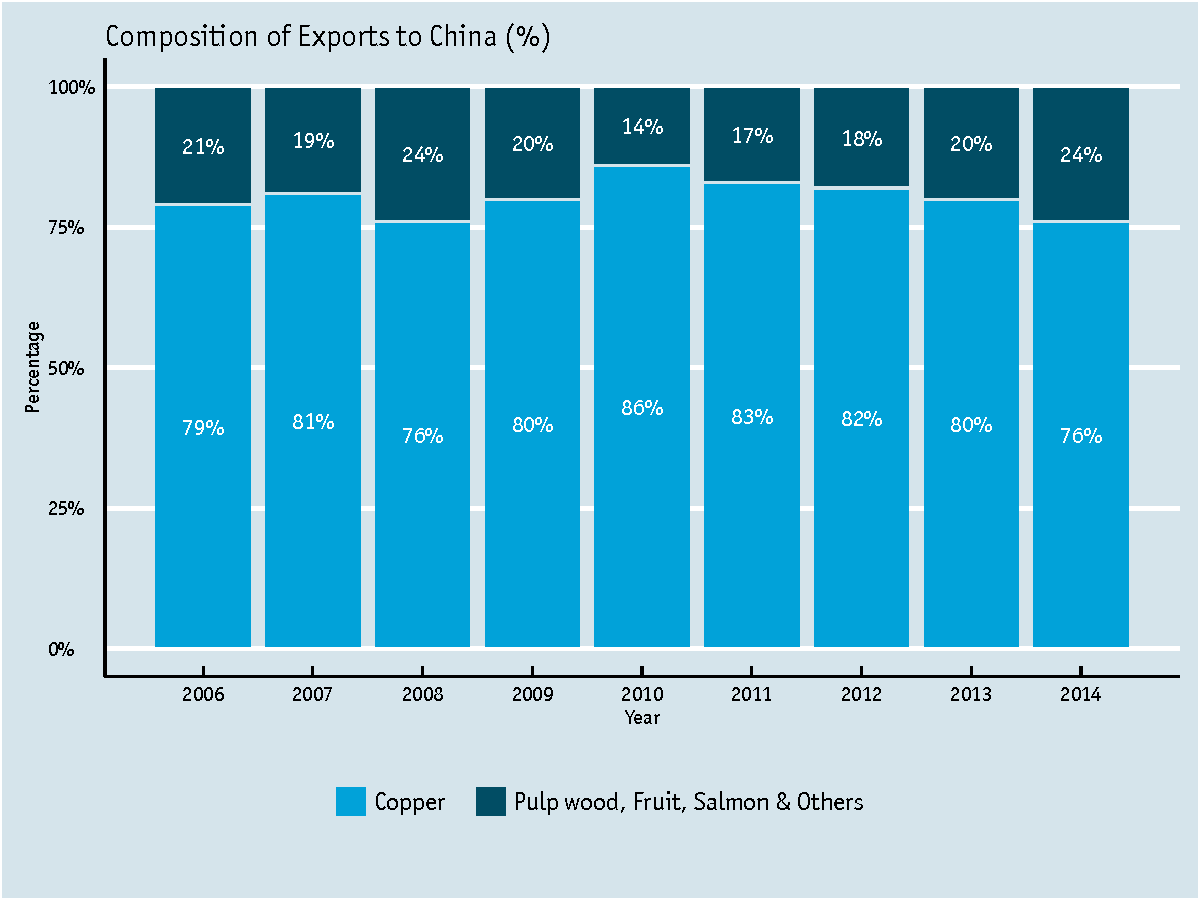
\includegraphics[width=0.55\linewidth]{figures/stacked_11-1} \end{center}

\section{Creating your own theme}\label{creating-your-own-theme-3}

As before, you can modify your plots a lot as \texttt{ggplot2} allows
many customisations. Here we present our original result shown at the
top of page.

\begin{Shaded}
\begin{Highlighting}[]
\NormalTok{fill <-}\StringTok{ }\KeywordTok{c}\NormalTok{(}\StringTok{"#40b8d0"}\NormalTok{, }\StringTok{"#b2d183"}\NormalTok{)}

\NormalTok{p4 <-}\StringTok{ }\KeywordTok{ggplot}\NormalTok{() +}\StringTok{ }
\StringTok{      }\KeywordTok{geom_bar}\NormalTok{(}\KeywordTok{aes}\NormalTok{(}\DataTypeTok{y =} \NormalTok{percentage, }\DataTypeTok{x =} \NormalTok{year, }\DataTypeTok{fill =} \NormalTok{product), }
\StringTok{        }\DataTypeTok{data =} \NormalTok{charts.data, }\DataTypeTok{stat=}\StringTok{"identity"}\NormalTok{) +}\StringTok{ }
\StringTok{      }\KeywordTok{geom_text}\NormalTok{(}\DataTypeTok{data=}\NormalTok{charts.data, }\KeywordTok{aes}\NormalTok{(}\DataTypeTok{x =} \NormalTok{year, }\DataTypeTok{y =} \NormalTok{pos, }
\StringTok{        }\DataTypeTok{label =} \KeywordTok{paste0}\NormalTok{(percentage,}\StringTok{"%"}\NormalTok{)), }
\StringTok{        }\DataTypeTok{colour=}\StringTok{"black"}\NormalTok{, }\DataTypeTok{family=}\StringTok{"Tahoma"}\NormalTok{, }\DataTypeTok{size=}\DecValTok{4}\NormalTok{) +}\StringTok{ }
\StringTok{      }\KeywordTok{scale_x_continuous}\NormalTok{(}\DataTypeTok{breaks=}\KeywordTok{seq}\NormalTok{(}\DecValTok{2006}\NormalTok{,}\DecValTok{2014}\NormalTok{,}\DecValTok{1}\NormalTok{)) +}\StringTok{ }
\StringTok{      }\KeywordTok{scale_y_continuous}\NormalTok{(}\DataTypeTok{labels =} \KeywordTok{dollar_format}\NormalTok{(}\DataTypeTok{suffix =} \StringTok{"%"}\NormalTok{, }\DataTypeTok{prefix =} \StringTok{""}\NormalTok{)) +}\StringTok{ }
\StringTok{      }\KeywordTok{labs}\NormalTok{(}\DataTypeTok{x=}\StringTok{"Year"}\NormalTok{, }\DataTypeTok{y=}\StringTok{"Percentage"}\NormalTok{) +}\StringTok{ }
\StringTok{      }\KeywordTok{ggtitle}\NormalTok{(}\StringTok{"Composition of Exports to China (%)"}\NormalTok{) +}\StringTok{ }
\StringTok{      }\KeywordTok{scale_fill_manual}\NormalTok{(}\DataTypeTok{values=}\NormalTok{fill) +}\StringTok{ }
\StringTok{      }\KeywordTok{theme}\NormalTok{(}\DataTypeTok{axis.line.x =} \KeywordTok{element_line}\NormalTok{(}\DataTypeTok{size=}\NormalTok{.}\DecValTok{5}\NormalTok{, }\DataTypeTok{colour =} \StringTok{"black"}\NormalTok{), }
\StringTok{        }\DataTypeTok{axis.line.y =} \KeywordTok{element_line}\NormalTok{(}\DataTypeTok{size=}\NormalTok{.}\DecValTok{5}\NormalTok{, }\DataTypeTok{colour =} \StringTok{"black"}\NormalTok{), }
\StringTok{        }\DataTypeTok{axis.text.x=}\KeywordTok{element_text}\NormalTok{(}\DataTypeTok{colour=}\StringTok{"black"}\NormalTok{, }\DataTypeTok{size =} \DecValTok{10}\NormalTok{), }
\StringTok{        }\DataTypeTok{axis.text.y=}\KeywordTok{element_text}\NormalTok{(}\DataTypeTok{colour=}\StringTok{"black"}\NormalTok{, }\DataTypeTok{size =} \DecValTok{10}\NormalTok{),}
\StringTok{        }\DataTypeTok{legend.key=}\KeywordTok{element_rect}\NormalTok{(}\DataTypeTok{fill=}\StringTok{"white"}\NormalTok{, }\DataTypeTok{colour=}\StringTok{"white"}\NormalTok{),}
\StringTok{        }\DataTypeTok{legend.position=}\StringTok{"bottom"}\NormalTok{, }\DataTypeTok{legend.direction=}\StringTok{"horizontal"}\NormalTok{, }
\StringTok{        }\DataTypeTok{legend.title =} \KeywordTok{element_blank}\NormalTok{(),}
\StringTok{        }\DataTypeTok{panel.grid.major =} \KeywordTok{element_line}\NormalTok{(}\DataTypeTok{colour =} \StringTok{"#d3d3d3"}\NormalTok{), }
\StringTok{        }\DataTypeTok{panel.grid.minor =} \KeywordTok{element_blank}\NormalTok{(), }
\StringTok{        }\DataTypeTok{panel.border =} \KeywordTok{element_blank}\NormalTok{(), }
\StringTok{        }\DataTypeTok{panel.background =} \KeywordTok{element_blank}\NormalTok{(),}
\StringTok{        }\DataTypeTok{plot.title =} \KeywordTok{element_text}\NormalTok{(}\DataTypeTok{size =} \DecValTok{14}\NormalTok{, }\DataTypeTok{family =} \StringTok{"Tahoma"}\NormalTok{, }\DataTypeTok{face =} \StringTok{"bold"}\NormalTok{), }
\StringTok{        }\DataTypeTok{text=}\KeywordTok{element_text}\NormalTok{(}\DataTypeTok{family=}\StringTok{"Tahoma"}\NormalTok{)) }
\NormalTok{p4}
\end{Highlighting}
\end{Shaded}

\begin{center}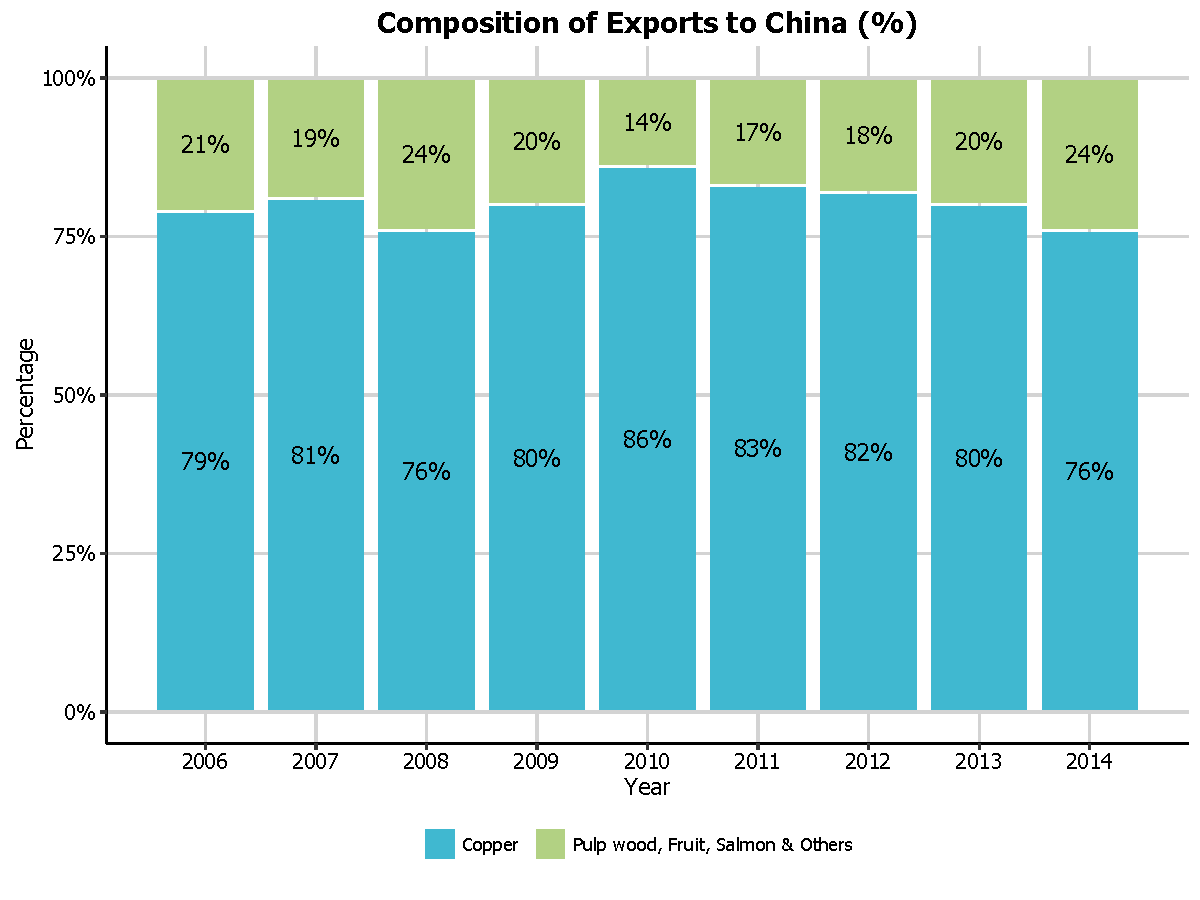
\includegraphics[width=0.55\linewidth]{figures/stacked_13-1} \end{center}
\chapter{Scatter Plots}\label{scatter-plots}

In this part, we will work towards creating the scatterplot below. We
will take you from a basic scatterplot and explain all the
customisations we add to the code step-by-step.

\begin{center}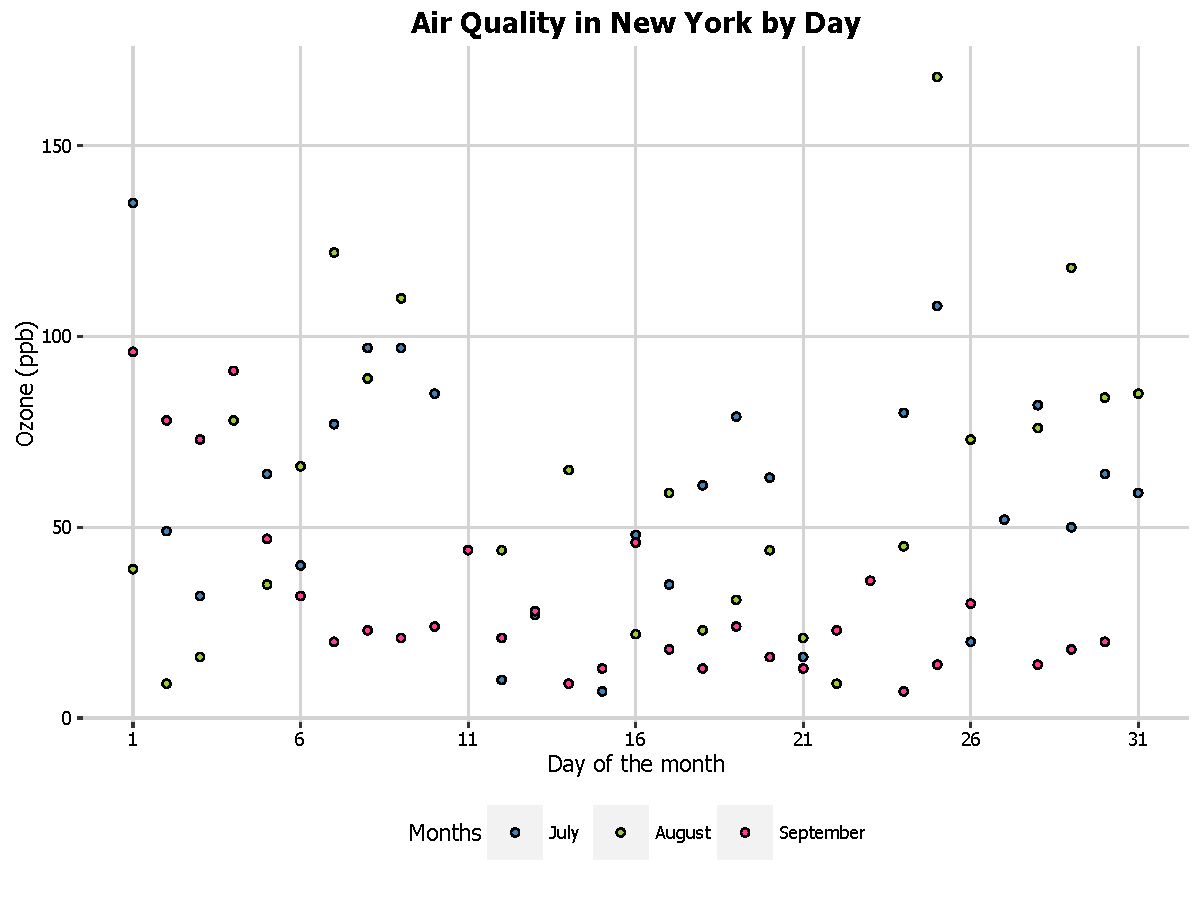
\includegraphics[width=0.55\linewidth]{figures/scatter_finalgraph-1} \end{center}

The first thing to do is load in the data, as below:

\begin{Shaded}
\begin{Highlighting}[]
\KeywordTok{library}\NormalTok{(ggplot2)}
\KeywordTok{library}\NormalTok{(ggthemes)}
\KeywordTok{library}\NormalTok{(extrafont)}
\KeywordTok{library}\NormalTok{(datasets)}
\KeywordTok{data}\NormalTok{(airquality)}
\end{Highlighting}
\end{Shaded}

We will then trim the data down to the final three months and turn the
\texttt{Month} variable into a labelled factor variable. We end up with
a new dataset called \texttt{aq\_trim}.

\begin{Shaded}
\begin{Highlighting}[]
\NormalTok{aq_trim <-}\StringTok{ }\NormalTok{airquality[}\KeywordTok{which}\NormalTok{(airquality$Month ==}\StringTok{ }\DecValTok{7} \NormalTok{|}
\NormalTok{airquality$Month ==}\StringTok{ }\DecValTok{8} \NormalTok{|}
\NormalTok{airquality$Month ==}\StringTok{ }\DecValTok{9}\NormalTok{), ]}
\NormalTok{aq_trim$Month <-}\StringTok{ }\KeywordTok{factor}\NormalTok{(aq_trim$Month, }
\DataTypeTok{labels =} \KeywordTok{c}\NormalTok{(}\StringTok{"July"}\NormalTok{, }\StringTok{"August"}\NormalTok{, }\StringTok{"September"}\NormalTok{))}
\end{Highlighting}
\end{Shaded}

\section{Basic scatterplot}\label{basic-scatterplot}

In order to initialise a scatterplot we tell ggplot that
\texttt{aq\_trim} is our data, and specify that our x-axis plots the
\texttt{Day} variable and our y-axis plots the \texttt{Ozone} variable.
We then instruct ggplot to render this as a scatterplot by adding the
\texttt{geom\_point()} option.

\begin{Shaded}
\begin{Highlighting}[]
\NormalTok{p5 <-}\StringTok{ }\KeywordTok{ggplot}\NormalTok{(aq_trim, }\KeywordTok{aes}\NormalTok{(}\DataTypeTok{x =} \NormalTok{Day, }\DataTypeTok{y =} \NormalTok{Ozone)) +}\StringTok{ }
\StringTok{      }\KeywordTok{geom_point}\NormalTok{()}
\NormalTok{p5}
\end{Highlighting}
\end{Shaded}

\begin{center}\includegraphics[width=0.55\linewidth]{figures/scatter_1-1} \end{center}

\section{Changing the shape of the data
points}\label{changing-the-shape-of-the-data-points}

Perhaps we want the data points to be a different shape than a solid
circle. We can change these by adding the \texttt{shape} argument to
\texttt{geom\_point}. An explanation of the allowed arguments for shape
are described in
\href{http://sape.inf.usi.ch/quick-reference/ggplot2/shape}{this
article}. In this case, we will use shape 21, which is a circle that
allows different colours for the outline and fill.

\begin{Shaded}
\begin{Highlighting}[]
\NormalTok{p5 <-}\StringTok{ }\KeywordTok{ggplot}\NormalTok{(aq_trim, }\KeywordTok{aes}\NormalTok{(}\DataTypeTok{x =} \NormalTok{Day, }\DataTypeTok{y =} \NormalTok{Ozone)) +}\StringTok{ }\KeywordTok{geom_point}\NormalTok{(}\DataTypeTok{shape =} \DecValTok{21}\NormalTok{)}
\NormalTok{p5}
\end{Highlighting}
\end{Shaded}

\begin{center}\includegraphics[width=0.55\linewidth]{figures/scatter_2-1} \end{center}

\section{Adjusting the axis scales}\label{adjusting-the-axis-scales}

To change the x-axis tick marks, we use the
\texttt{scale\_x\_continuous} option. Similarly, to change the y-axis we
use the \texttt{scale\_y\_continuous} option. Here we will change the
x-axis to every 5 days, rather than 10, and change the range from 1 to
31 (as 0 is not a valid value for this variable).

\begin{Shaded}
\begin{Highlighting}[]
\NormalTok{p5 <-}\StringTok{ }\NormalTok{p5 +}\StringTok{ }\KeywordTok{scale_x_continuous}\NormalTok{(}\DataTypeTok{breaks =} \KeywordTok{seq}\NormalTok{(}\DecValTok{1}\NormalTok{, }\DecValTok{31}\NormalTok{, }\DecValTok{5}\NormalTok{))}
\NormalTok{p5}
\end{Highlighting}
\end{Shaded}

\begin{center}\includegraphics[width=0.55\linewidth]{figures/scatter_3-1} \end{center}

\section{Adjusting axis labels \& adding
title}\label{adjusting-axis-labels-adding-title-3}

To add a title, we include the option \texttt{ggtitle} and include the
name of the graph as a string argument. To change the axis names we add
\texttt{x} and \texttt{y} arguments to the \texttt{labs} command.

\begin{Shaded}
\begin{Highlighting}[]
\NormalTok{p5 <-}\StringTok{ }\NormalTok{p5 +}\StringTok{ }\KeywordTok{ggtitle}\NormalTok{(}\StringTok{"Air Quality in New York by Day"}\NormalTok{) +}\StringTok{ }
\StringTok{      }\KeywordTok{labs}\NormalTok{(}\DataTypeTok{x =} \StringTok{"Day of the month"}\NormalTok{, }\DataTypeTok{y =} \StringTok{"Ozone (ppb)"}\NormalTok{) }
\NormalTok{p5}
\end{Highlighting}
\end{Shaded}

\begin{center}\includegraphics[width=0.55\linewidth]{figures/scatter_4-1} \end{center}

\section{Adjusting the colour
palette}\label{adjusting-the-colour-palette}

There are a few options for adjusting the colour. The most simple is to
make every point one fixed colour. You can reference colours by name,
with the full list of colours recognised by R
\href{http://www.stat.columbia.edu/~tzheng/files/Rcolor.pdf}{here}.
Let's try making the outline \texttt{mediumvioletred} and the fill
\texttt{springgreen}.

\begin{Shaded}
\begin{Highlighting}[]
\NormalTok{p5 <-}\StringTok{ }\KeywordTok{ggplot}\NormalTok{(aq_trim, }\KeywordTok{aes}\NormalTok{(}\DataTypeTok{x =} \NormalTok{Day, }\DataTypeTok{y =} \NormalTok{Ozone)) +}\StringTok{ }
\StringTok{      }\KeywordTok{geom_point}\NormalTok{(}\DataTypeTok{shape =} \DecValTok{21}\NormalTok{, }\DataTypeTok{colour =} \StringTok{"mediumvioletred"}\NormalTok{, }\DataTypeTok{fill =} \StringTok{"springgreen"}\NormalTok{) +}
\StringTok{      }\KeywordTok{ggtitle}\NormalTok{(}\StringTok{"Air Quality in New York by Day"}\NormalTok{) +}\StringTok{ }
\StringTok{      }\KeywordTok{labs}\NormalTok{(}\DataTypeTok{x =} \StringTok{"Day of the month"}\NormalTok{, }\DataTypeTok{y =} \StringTok{"Ozone (ppb)"}\NormalTok{) +}
\StringTok{      }\KeywordTok{scale_x_continuous}\NormalTok{(}\DataTypeTok{breaks =} \KeywordTok{seq}\NormalTok{(}\DecValTok{1}\NormalTok{, }\DecValTok{31}\NormalTok{, }\DecValTok{5}\NormalTok{)) }
\NormalTok{p5}
\end{Highlighting}
\end{Shaded}

\begin{center}\includegraphics[width=0.55\linewidth]{figures/scatter_5-1} \end{center}

You can change the colours using specific HEX codes instead. Here we
have made the outline \#000000 (black) and the fill ``\#40b8d0 (vivid
cyan).

\begin{Shaded}
\begin{Highlighting}[]
\NormalTok{p5 <-}\StringTok{ }\KeywordTok{ggplot}\NormalTok{(aq_trim, }\KeywordTok{aes}\NormalTok{(}\DataTypeTok{x =} \NormalTok{Day, }\DataTypeTok{y =} \NormalTok{Ozone)) +}\StringTok{ }
\StringTok{      }\KeywordTok{geom_point}\NormalTok{(}\DataTypeTok{shape =} \DecValTok{21}\NormalTok{, }\DataTypeTok{colour =} \StringTok{"#000000"}\NormalTok{, }\DataTypeTok{fill =} \StringTok{"#40b8d0"}\NormalTok{) +}
\StringTok{      }\KeywordTok{ggtitle}\NormalTok{(}\StringTok{"Air Quality in New York by Day"}\NormalTok{) +}\StringTok{ }
\StringTok{      }\KeywordTok{labs}\NormalTok{(}\DataTypeTok{x =} \StringTok{"Day of the month"}\NormalTok{, }\DataTypeTok{y =} \StringTok{"Ozone (ppb)"}\NormalTok{) +}
\StringTok{      }\KeywordTok{scale_x_continuous}\NormalTok{(}\DataTypeTok{breaks =} \KeywordTok{seq}\NormalTok{(}\DecValTok{1}\NormalTok{, }\DecValTok{31}\NormalTok{, }\DecValTok{5}\NormalTok{))}
\NormalTok{p5}
\end{Highlighting}
\end{Shaded}

\begin{center}\includegraphics[width=0.55\linewidth]{figures/scatter_6-1} \end{center}

You can also change the colour of the data points according to the
levels of another variable. This can be done either as a continuous
gradient, or as a levels of a factor variable. Let's change the colour
by the values of temperature:

\begin{Shaded}
\begin{Highlighting}[]
\NormalTok{p5 <-}\StringTok{ }\KeywordTok{ggplot}\NormalTok{(aq_trim, }\KeywordTok{aes}\NormalTok{(}\DataTypeTok{x =} \NormalTok{Day, }\DataTypeTok{y =} \NormalTok{Ozone, }\DataTypeTok{fill =} \NormalTok{Temp)) +}\StringTok{ }
\StringTok{      }\KeywordTok{geom_point}\NormalTok{(}\DataTypeTok{shape =} \DecValTok{21}\NormalTok{) +}
\StringTok{      }\KeywordTok{ggtitle}\NormalTok{(}\StringTok{"Air Quality in New York by Day"}\NormalTok{) +}\StringTok{ }
\StringTok{      }\KeywordTok{labs}\NormalTok{(}\DataTypeTok{x =} \StringTok{"Day of the month"}\NormalTok{, }\DataTypeTok{y =} \StringTok{"Ozone (ppb)"}\NormalTok{) +}
\StringTok{      }\KeywordTok{scale_x_continuous}\NormalTok{(}\DataTypeTok{breaks =} \KeywordTok{seq}\NormalTok{(}\DecValTok{1}\NormalTok{, }\DecValTok{31}\NormalTok{, }\DecValTok{5}\NormalTok{))}
\NormalTok{p5}
\end{Highlighting}
\end{Shaded}

\begin{center}\includegraphics[width=0.55\linewidth]{figures/scatter_7-1} \end{center}

We can change the gradient's colours by adding the
\texttt{scale\_fill\_continuous} option. The \texttt{low} and
\texttt{high} arguments specify the range of colours the gradient should
transition between.

\begin{Shaded}
\begin{Highlighting}[]
\NormalTok{p5 <-}\StringTok{  }\NormalTok{p5 +}\StringTok{ }\KeywordTok{scale_fill_continuous}\NormalTok{(}\DataTypeTok{low =} \StringTok{"plum1"}\NormalTok{, }\DataTypeTok{high =} \StringTok{"purple4"}\NormalTok{)}
\NormalTok{p5}
\end{Highlighting}
\end{Shaded}

\begin{center}\includegraphics[width=0.55\linewidth]{figures/scatter_8-1} \end{center}

We can see that higher temperatures seem to have higher ozone levels.

Let's now change the colours of the data points by a factor variable,
\texttt{Month}.

\begin{Shaded}
\begin{Highlighting}[]
\NormalTok{p5 <-}\StringTok{ }\KeywordTok{ggplot}\NormalTok{(aq_trim, }\KeywordTok{aes}\NormalTok{(}\DataTypeTok{x =} \NormalTok{Day, }\DataTypeTok{y =} \NormalTok{Ozone, }\DataTypeTok{fill =} \NormalTok{Month)) +}\StringTok{ }
\StringTok{      }\KeywordTok{geom_point}\NormalTok{(}\DataTypeTok{shape =} \DecValTok{21}\NormalTok{) +}
\StringTok{      }\KeywordTok{ggtitle}\NormalTok{(}\StringTok{"Air Quality in New York by Day"}\NormalTok{) +}\StringTok{ }
\StringTok{      }\KeywordTok{labs}\NormalTok{(}\DataTypeTok{x =} \StringTok{"Day of the month"}\NormalTok{, }\DataTypeTok{y =} \StringTok{"Ozone (ppb)"}\NormalTok{) +}
\StringTok{      }\KeywordTok{scale_x_continuous}\NormalTok{(}\DataTypeTok{breaks =} \KeywordTok{seq}\NormalTok{(}\DecValTok{1}\NormalTok{, }\DecValTok{31}\NormalTok{, }\DecValTok{5}\NormalTok{))}
\NormalTok{p5}
\end{Highlighting}
\end{Shaded}

\begin{center}\includegraphics[width=0.55\linewidth]{figures/scatter_9-1} \end{center}

Again, we can change the colours of these data points, this time using
\texttt{scale\_fill\_manual}.

\begin{Shaded}
\begin{Highlighting}[]
\NormalTok{fill =}\StringTok{ }\KeywordTok{c}\NormalTok{(}\StringTok{"steelblue"}\NormalTok{, }\StringTok{"yellowgreen"}\NormalTok{, }\StringTok{"violetred1"}\NormalTok{)}

\NormalTok{p5 <-}\StringTok{ }\NormalTok{p5 +}\StringTok{ }\KeywordTok{scale_fill_manual}\NormalTok{(}\DataTypeTok{values =} \NormalTok{fill)}
\NormalTok{p5}
\end{Highlighting}
\end{Shaded}

\begin{center}\includegraphics[width=0.55\linewidth]{figures/scatter_10-1} \end{center}

\section{Adjusting legend
position}\label{adjusting-legend-position-3}

To adjust the position of the legend from the default spot of right of
the graph, we add the \texttt{theme} option and specify the
\texttt{legend.position\ =\ "bottom"} argument. We can also change the
legend shape using the \texttt{legend.direction\ =\ "horizontal"}
argument.

\begin{Shaded}
\begin{Highlighting}[]
\NormalTok{p5 <-}\StringTok{ }\NormalTok{p5 +}\StringTok{ }\KeywordTok{theme}\NormalTok{(}\DataTypeTok{legend.position =} \StringTok{"bottom"}\NormalTok{, }\DataTypeTok{legend.direction =} \StringTok{"horizontal"}\NormalTok{)}
\NormalTok{p5}
\end{Highlighting}
\end{Shaded}

\begin{center}\includegraphics[width=0.55\linewidth]{figures/scatter_11-1} \end{center}

\section{Using the white theme}\label{using-the-white-theme-4}

As explained in the previous posts, we can also change the overall look
of the plot using themes. We'll start using a simple theme customisation
by adding \texttt{theme\_bw()} after \texttt{ggplot()}. As you can see,
we can further tweak the graph using the \texttt{theme} option, which
we've used so far to change the legend.

\begin{Shaded}
\begin{Highlighting}[]
\NormalTok{p5 <-}\StringTok{ }\KeywordTok{ggplot}\NormalTok{(aq_trim, }\KeywordTok{aes}\NormalTok{(}\DataTypeTok{x =} \NormalTok{Day, }\DataTypeTok{y =} \NormalTok{Ozone, }\DataTypeTok{fill =} \NormalTok{Month)) +}\StringTok{ }\KeywordTok{theme_bw}\NormalTok{() +}
\StringTok{      }\KeywordTok{geom_point}\NormalTok{(}\DataTypeTok{shape =} \DecValTok{21}\NormalTok{) +}
\StringTok{      }\KeywordTok{ggtitle}\NormalTok{(}\StringTok{"Air Quality in New York by Day"}\NormalTok{) +}\StringTok{ }
\StringTok{      }\KeywordTok{labs}\NormalTok{(}\DataTypeTok{x =} \StringTok{"Day of the month"}\NormalTok{, }\DataTypeTok{y =} \StringTok{"Ozone (ppb)"}\NormalTok{, }\DataTypeTok{fill =} \StringTok{"Months"}\NormalTok{) +}
\StringTok{      }\KeywordTok{scale_x_continuous}\NormalTok{(}\DataTypeTok{breaks =} \KeywordTok{seq}\NormalTok{(}\DecValTok{1}\NormalTok{, }\DecValTok{31}\NormalTok{, }\DecValTok{5}\NormalTok{)) +}
\StringTok{      }\KeywordTok{scale_fill_manual}\NormalTok{(}\DataTypeTok{values =} \NormalTok{fill) +}
\StringTok{      }\KeywordTok{scale_size}\NormalTok{(}\DataTypeTok{range =} \KeywordTok{c}\NormalTok{(}\DecValTok{1}\NormalTok{, }\DecValTok{10}\NormalTok{)) +}
\StringTok{      }\KeywordTok{theme}\NormalTok{(}\DataTypeTok{legend.position=}\StringTok{"bottom"}\NormalTok{, }\DataTypeTok{legend.direction=}\StringTok{"horizontal"}\NormalTok{)}
\NormalTok{p5}
\end{Highlighting}
\end{Shaded}

\begin{center}\includegraphics[width=0.55\linewidth]{figures/scatter_12-1} \end{center}

\section{Creating an XKCD style
chart}\label{creating-an-xkcd-style-chart-4}

Of course, you may want to create your own themes as well.
\texttt{ggplot2} allows for a very high degree of customisation,
including allowing you to use imported fonts. Below is an example of a
theme Mauricio was able to create which mimics the visual style of
\href{http://xkcd.com/}{XKCD}. In order to create this chart, you first
need to import the XKCD font, install it on your machine and load it
into R using the \texttt{extrafont} package. These instructions are
taken from
\href{https://www.google.com.au/url?sa=t\&rct=j\&q=\&esrc=s\&source=web\&cd=1\&ved=0ahUKEwiWzafchdPJAhVBpJQKHe_LDT8QFggbMAA\&url=https\%3A\%2F\%2Fcran.r-project.org\%2Fweb\%2Fpackages\%2Fxkcd\%2Fvignettes\%2Fxkcd-intro.pdf\&usg=AFQjCNE-KciGY14e-Q1buYIVmTFC0ht__Q\&sig2=DZUwkvIHwfNWtTtkcz94jg}{here}:

\begin{Shaded}
\begin{Highlighting}[]
\KeywordTok{library}\NormalTok{(extrafont)}

\KeywordTok{download.file}\NormalTok{(}\StringTok{"http://simonsoftware.se/other/xkcd.ttf"}\NormalTok{, }\DataTypeTok{dest=}\StringTok{"xkcd.ttf"}\NormalTok{, }
	\DataTypeTok{mode=}\StringTok{"wb"}\NormalTok{)}
\KeywordTok{system}\NormalTok{(}\StringTok{"mkdir ~/.fonts"}\NormalTok{)}
\KeywordTok{system}\NormalTok{(}\StringTok{"cp xkcd.ttf  ~/.fonts"}\NormalTok{)}
\KeywordTok{font_import}\NormalTok{(}\DataTypeTok{paths =} \StringTok{"~/.fonts"}\NormalTok{, }\DataTypeTok{pattern=}\StringTok{"[X/x]kcd"}\NormalTok{)}
\KeywordTok{fonts}\NormalTok{()}
\KeywordTok{loadfonts}\NormalTok{()}
\end{Highlighting}
\end{Shaded}

You can then create your graph:

\begin{Shaded}
\begin{Highlighting}[]
\NormalTok{fill <-}\StringTok{ }\KeywordTok{c}\NormalTok{(}\StringTok{"#56B4E9"}\NormalTok{, }\StringTok{"#F0E442"}\NormalTok{, }\StringTok{"violetred1"}\NormalTok{)}

\NormalTok{p5 <-}\StringTok{ }\KeywordTok{ggplot}\NormalTok{(aq_trim, }\KeywordTok{aes}\NormalTok{(}\DataTypeTok{x =} \NormalTok{Day, }\DataTypeTok{y =} \NormalTok{Ozone, }\DataTypeTok{fill =} \NormalTok{Month)) +}\StringTok{ }
\StringTok{      }\KeywordTok{geom_point}\NormalTok{(}\DataTypeTok{shape =} \DecValTok{21}\NormalTok{) +}
\StringTok{      }\KeywordTok{ggtitle}\NormalTok{(}\StringTok{"Air Quality in New York by Day"}\NormalTok{) +}\StringTok{ }
\StringTok{      }\KeywordTok{labs}\NormalTok{(}\DataTypeTok{x =} \StringTok{"Day of the month"}\NormalTok{, }\DataTypeTok{y =} \StringTok{"Ozone (ppb)"}\NormalTok{, }\DataTypeTok{fill =} \StringTok{"Months"}\NormalTok{) +}
\StringTok{      }\KeywordTok{scale_x_continuous}\NormalTok{(}\DataTypeTok{breaks =} \KeywordTok{seq}\NormalTok{(}\DecValTok{1}\NormalTok{, }\DecValTok{31}\NormalTok{, }\DecValTok{5}\NormalTok{)) +}
\StringTok{      }\KeywordTok{scale_fill_manual}\NormalTok{(}\DataTypeTok{values =} \NormalTok{fill) +}
\StringTok{      }\KeywordTok{scale_size}\NormalTok{(}\DataTypeTok{range =} \KeywordTok{c}\NormalTok{(}\DecValTok{1}\NormalTok{, }\DecValTok{10}\NormalTok{)) +}
\StringTok{      }\KeywordTok{theme}\NormalTok{(}\DataTypeTok{axis.line.x =} \KeywordTok{element_line}\NormalTok{(}\DataTypeTok{size=}\DecValTok{1}\NormalTok{, }\DataTypeTok{colour =} \StringTok{"black"}\NormalTok{),}
\StringTok{        }\DataTypeTok{axis.line.y =} \KeywordTok{element_line}\NormalTok{(}\DataTypeTok{size=}\DecValTok{1}\NormalTok{, }\DataTypeTok{colour =} \StringTok{"black"}\NormalTok{),}
\StringTok{        }\DataTypeTok{axis.text.x=}\KeywordTok{element_text}\NormalTok{(}\DataTypeTok{colour=}\StringTok{"black"}\NormalTok{, }\DataTypeTok{size =} \DecValTok{10}\NormalTok{), }
\StringTok{        }\DataTypeTok{axis.text.y=}\KeywordTok{element_text}\NormalTok{(}\DataTypeTok{colour=}\StringTok{"black"}\NormalTok{, }\DataTypeTok{size =} \DecValTok{10}\NormalTok{), }
\StringTok{        }\DataTypeTok{legend.position=}\StringTok{"bottom"}\NormalTok{, }\DataTypeTok{legend.direction=}\StringTok{"horizontal"}\NormalTok{,}
\StringTok{        }\DataTypeTok{panel.grid.major =} \KeywordTok{element_blank}\NormalTok{(),}
\StringTok{        }\DataTypeTok{panel.grid.minor =} \KeywordTok{element_blank}\NormalTok{(), }
\StringTok{        }\DataTypeTok{panel.border =} \KeywordTok{element_blank}\NormalTok{(),}
\StringTok{        }\DataTypeTok{panel.background =} \KeywordTok{element_blank}\NormalTok{(),}
\StringTok{        }\DataTypeTok{plot.title=}\KeywordTok{element_text}\NormalTok{(}\DataTypeTok{family=}\StringTok{"xkcd-Regular"}\NormalTok{), }
\StringTok{        }\DataTypeTok{text=}\KeywordTok{element_text}\NormalTok{(}\DataTypeTok{family=}\StringTok{"xkcd-Regular"}\NormalTok{)) }
\NormalTok{p5}
\end{Highlighting}
\end{Shaded}

\begin{center}\includegraphics[width=0.55\linewidth]{figures/scatter_13-1} \end{center}

\section{\texorpdfstring{Using `The Economist'
theme}{Using The Economist theme}}\label{using-the-economist-theme-4}

There are a wider range of pre-built themes available as part of the
\texttt{ggthemes} package (more information on these
\href{https://cran.r-project.org/web/packages/ggthemes/vignettes/ggthemes.html}{here}).
Below we've applied \texttt{theme\_economist()}, which approximates
graphs in the Economist magazine.

\begin{Shaded}
\begin{Highlighting}[]
\NormalTok{p5 <-}\StringTok{ }\KeywordTok{ggplot}\NormalTok{(aq_trim, }\KeywordTok{aes}\NormalTok{(}\DataTypeTok{x =} \NormalTok{Day, }\DataTypeTok{y =} \NormalTok{Ozone, }\DataTypeTok{fill =} \NormalTok{Month)) +}
\StringTok{      }\KeywordTok{scale_fill_economist}\NormalTok{() +}
\StringTok{      }\KeywordTok{geom_point}\NormalTok{(}\DataTypeTok{shape =} \DecValTok{21}\NormalTok{) +}
\StringTok{      }\KeywordTok{ggtitle}\NormalTok{(}\StringTok{"Air Quality in New York by Day"}\NormalTok{) +}\StringTok{ }
\StringTok{      }\KeywordTok{labs}\NormalTok{(}\DataTypeTok{x =} \StringTok{"Day of the month"}\NormalTok{, }\DataTypeTok{y =} \StringTok{"Ozone (ppb)"}\NormalTok{, }\DataTypeTok{fill =} \StringTok{"Months"}\NormalTok{) +}
\StringTok{      }\KeywordTok{scale_x_continuous}\NormalTok{(}\DataTypeTok{breaks =} \KeywordTok{seq}\NormalTok{(}\DecValTok{1}\NormalTok{, }\DecValTok{31}\NormalTok{, }\DecValTok{5}\NormalTok{)) +}
\StringTok{      }\KeywordTok{scale_size}\NormalTok{(}\DataTypeTok{range =} \KeywordTok{c}\NormalTok{(}\DecValTok{1}\NormalTok{, }\DecValTok{10}\NormalTok{)) +}
\StringTok{      }\KeywordTok{theme_economist}\NormalTok{() +}\StringTok{ }
\StringTok{      }\KeywordTok{theme}\NormalTok{(}\DataTypeTok{axis.line.x =} \KeywordTok{element_line}\NormalTok{(}\DataTypeTok{size=}\NormalTok{.}\DecValTok{5}\NormalTok{, }\DataTypeTok{colour =} \StringTok{"black"}\NormalTok{), }
\StringTok{        }\DataTypeTok{axis.line.y =} \KeywordTok{element_line}\NormalTok{(}\DataTypeTok{size=}\NormalTok{.}\DecValTok{5}\NormalTok{, }\DataTypeTok{colour =} \StringTok{"black"}\NormalTok{), }
\StringTok{        }\DataTypeTok{axis.title =} \KeywordTok{element_text}\NormalTok{(}\DataTypeTok{size =} \DecValTok{12}\NormalTok{),}
\StringTok{        }\DataTypeTok{legend.position =} \StringTok{"bottom"}\NormalTok{, }\DataTypeTok{legend.direction =} \StringTok{"horizontal"}\NormalTok{,}
\StringTok{        }\DataTypeTok{legend.text =} \KeywordTok{element_text}\NormalTok{(}\DataTypeTok{size =} \DecValTok{9}\NormalTok{),}
\StringTok{        }\DataTypeTok{legend.title=}\KeywordTok{element_text}\NormalTok{(}\DataTypeTok{face =} \StringTok{"bold"}\NormalTok{, }\DataTypeTok{size =} \DecValTok{9}\NormalTok{),}
\StringTok{        }\DataTypeTok{text =} \KeywordTok{element_text}\NormalTok{(}\DataTypeTok{family =} \StringTok{"Tahoma"}\NormalTok{),  }
\StringTok{        }\DataTypeTok{plot.title =} \KeywordTok{element_text}\NormalTok{(}\DataTypeTok{family=}\StringTok{"Tahoma"}\NormalTok{))}
\NormalTok{p5}
\end{Highlighting}
\end{Shaded}

\begin{center}\includegraphics[width=0.55\linewidth]{figures/scatter_14-1} \end{center}

\section{Creating your own theme}\label{creating-your-own-theme-4}

As before, you can modify your plots a lot as \texttt{ggplot2} allows
many customisations. Here we present our original result shown at the
top of page.

\begin{Shaded}
\begin{Highlighting}[]
\NormalTok{fill =}\StringTok{ }\KeywordTok{c}\NormalTok{(}\StringTok{"steelblue"}\NormalTok{, }\StringTok{"yellowgreen"}\NormalTok{, }\StringTok{"violetred1"}\NormalTok{)}

\NormalTok{p5 <-}\StringTok{ }\KeywordTok{ggplot}\NormalTok{(aq_trim, }\KeywordTok{aes}\NormalTok{(}\DataTypeTok{x =} \NormalTok{Day, }\DataTypeTok{y =} \NormalTok{Ozone, }\DataTypeTok{fill =} \NormalTok{Month)) +}
\StringTok{      }\KeywordTok{geom_point}\NormalTok{(}\DataTypeTok{shape =} \DecValTok{21}\NormalTok{) +}
\StringTok{      }\KeywordTok{ggtitle}\NormalTok{(}\StringTok{"Air Quality in New York by Day"}\NormalTok{) +}\StringTok{ }
\StringTok{      }\KeywordTok{labs}\NormalTok{(}\DataTypeTok{x =} \StringTok{"Day of the month"}\NormalTok{, }\DataTypeTok{y =} \StringTok{"Ozone (ppb)"}\NormalTok{, }\DataTypeTok{fill =} \StringTok{"Months"}\NormalTok{) +}
\StringTok{      }\KeywordTok{scale_x_continuous}\NormalTok{(}\DataTypeTok{breaks =} \KeywordTok{seq}\NormalTok{(}\DecValTok{1}\NormalTok{, }\DecValTok{31}\NormalTok{, }\DecValTok{5}\NormalTok{)) +}
\StringTok{      }\KeywordTok{scale_size}\NormalTok{(}\DataTypeTok{range =} \KeywordTok{c}\NormalTok{(}\DecValTok{1}\NormalTok{, }\DecValTok{10}\NormalTok{)) +}
\StringTok{      }\KeywordTok{scale_fill_manual}\NormalTok{(}\DataTypeTok{values =} \NormalTok{fill) +}
\StringTok{      }\KeywordTok{theme}\NormalTok{(}\DataTypeTok{axis.line.x =} \KeywordTok{element_line}\NormalTok{(}\DataTypeTok{size=}\DecValTok{1}\NormalTok{, }\DataTypeTok{colour =} \StringTok{"black"}\NormalTok{), }
\StringTok{        }\DataTypeTok{axis.line.y =} \KeywordTok{element_line}\NormalTok{(}\DataTypeTok{size=}\DecValTok{1}\NormalTok{, }\DataTypeTok{colour =} \StringTok{"black"}\NormalTok{), }
\StringTok{        }\DataTypeTok{axis.text.x=}\KeywordTok{element_text}\NormalTok{(}\DataTypeTok{colour=}\StringTok{"black"}\NormalTok{, }\DataTypeTok{size =} \DecValTok{9}\NormalTok{), }
\StringTok{        }\DataTypeTok{axis.text.y=}\KeywordTok{element_text}\NormalTok{(}\DataTypeTok{colour=}\StringTok{"black"}\NormalTok{, }\DataTypeTok{size =} \DecValTok{9}\NormalTok{),  }
\StringTok{        }\DataTypeTok{legend.position =} \StringTok{"bottom"}\NormalTok{, }\DataTypeTok{legend.direction =} \StringTok{"horizontal"}\NormalTok{,}
\StringTok{        }\DataTypeTok{panel.grid.major =} \KeywordTok{element_line}\NormalTok{(}\DataTypeTok{colour =} \StringTok{"#d3d3d3"}\NormalTok{), }
\StringTok{        }\DataTypeTok{panel.grid.minor =} \KeywordTok{element_blank}\NormalTok{(), }
\StringTok{        }\DataTypeTok{panel.border =} \KeywordTok{element_blank}\NormalTok{(), }\DataTypeTok{panel.background =} \KeywordTok{element_blank}\NormalTok{(),}
\StringTok{        }\DataTypeTok{plot.title =} \KeywordTok{element_text}\NormalTok{(}\DataTypeTok{size =} \DecValTok{14}\NormalTok{, }\DataTypeTok{family =} \StringTok{"Tahoma"}\NormalTok{, }
\StringTok{        }\DataTypeTok{face =} \StringTok{"bold"}\NormalTok{),}
\StringTok{        }\DataTypeTok{text=}\KeywordTok{element_text}\NormalTok{(}\DataTypeTok{family=}\StringTok{"Tahoma"}\NormalTok{)) }
\NormalTok{p5}
\end{Highlighting}
\end{Shaded}

\begin{center}\includegraphics[width=0.55\linewidth]{figures/scatter_15-1} \end{center}
\chapter{Weighted Scatter Plots}\label{weighted-scatter-plots}

The first thing to do is load in the data, as below:

\begin{Shaded}
\begin{Highlighting}[]
\KeywordTok{rm}\NormalTok{(}\DataTypeTok{list =} \KeywordTok{ls}\NormalTok{())}
\KeywordTok{library}\NormalTok{(datasets)}
\KeywordTok{library}\NormalTok{(ggplot2)}
\KeywordTok{data}\NormalTok{(airquality)}
\end{Highlighting}
\end{Shaded}

We will then trim the data down to the final three months and turn the
\texttt{Month} variable into a labelled factor variable. We end up with
a new dataset called \texttt{aq\_trim}.

\begin{Shaded}
\begin{Highlighting}[]
\NormalTok{aq_trim <-}\StringTok{ }\NormalTok{airquality[}\KeywordTok{which}\NormalTok{(airquality$Month ==}\StringTok{ }\DecValTok{7} \NormalTok{|}
\NormalTok{airquality$Month ==}\StringTok{ }\DecValTok{8} \NormalTok{|}
\NormalTok{airquality$Month ==}\StringTok{ }\DecValTok{9}\NormalTok{), ]}
\NormalTok{aq_trim$Month <-}\StringTok{ }\KeywordTok{factor}\NormalTok{(aq_trim$Month, }
\DataTypeTok{labels =} \KeywordTok{c}\NormalTok{(}\StringTok{"July"}\NormalTok{, }\StringTok{"August"}\NormalTok{, }\StringTok{"September"}\NormalTok{))}
\end{Highlighting}
\end{Shaded}

In this part, we will work towards creating the weighted scatterplot
below. We will take you from a basic scatterplot and explain all the
customisations we add to the code step-by-step.

\begin{center}\includegraphics[width=0.55\linewidth]{0_all_posts_pdf/wscatter_finalgraph-1} \end{center}

\section{Basic weighted
scatterplot}\label{basic-weighted-scatterplot}

Let's start really slowly by revisiting how to create a basic
scatterplot. In order to initialise this plot we tell ggplot that
\texttt{aq\_trim} is our data, and specify that our x-axis plots the
\texttt{Day} variable and our y-axis plots the \texttt{Ozone} variable.
We then instruct ggplot to render this as a scatterplot by adding the
\texttt{geom\_point()} option.

\begin{Shaded}
\begin{Highlighting}[]
\NormalTok{p6 <-}\StringTok{ }\KeywordTok{ggplot}\NormalTok{(aq_trim, }\KeywordTok{aes}\NormalTok{(}\DataTypeTok{x =} \NormalTok{Day, }\DataTypeTok{y =} \NormalTok{Ozone)) +}\StringTok{ }
\StringTok{      }\KeywordTok{geom_point}\NormalTok{()}
\NormalTok{p6}
\end{Highlighting}
\end{Shaded}

\begin{center}\includegraphics[width=0.55\linewidth]{0_all_posts_pdf/wscatter_1-1} \end{center}

In order to turn this into a weighted scatterplot, we simply add the
\texttt{size} argument to \texttt{ggplot(aes())}. In this case, we want
to weight the points by the \texttt{Wind} variable.

\begin{Shaded}
\begin{Highlighting}[]
\NormalTok{p6 <-}\StringTok{ }\KeywordTok{ggplot}\NormalTok{(aq_trim, }\KeywordTok{aes}\NormalTok{(}\DataTypeTok{x =} \NormalTok{Day, }\DataTypeTok{y =} \NormalTok{Ozone, }\DataTypeTok{size =} \NormalTok{Wind)) +}\StringTok{ }
\StringTok{      }\KeywordTok{geom_point}\NormalTok{()}
\NormalTok{p6}
\end{Highlighting}
\end{Shaded}

\begin{center}\includegraphics[width=0.55\linewidth]{0_all_posts_pdf/wscatter_2-1} \end{center}

You can see we already have an interesting looking pattern, where days
with higher wind speed tend to have lower ozone (or in other words,
better air quality). Now let's make it beautiful!

\section{Changing the shape of the data
points}\label{changing-the-shape-of-the-data-points-1}

Perhaps we want the data points to be a different shape than a solid
circle. We can change these by adding the \texttt{shape} argument to
\texttt{geom\_point}. An explanation of the allowed arguments for shape
are described in
\href{http://sape.inf.usi.ch/quick-reference/ggplot2/shape}{this
article}. In this case, we will use shape 21, which is a circle that
allows different colours for the outline and fill.

\begin{Shaded}
\begin{Highlighting}[]
\NormalTok{p6 <-}\StringTok{ }\KeywordTok{ggplot}\NormalTok{(aq_trim, }\KeywordTok{aes}\NormalTok{(}\DataTypeTok{x =} \NormalTok{Day, }\DataTypeTok{y =} \NormalTok{Ozone, }\DataTypeTok{size =} \NormalTok{Wind)) +}\StringTok{ }
\StringTok{      }\KeywordTok{geom_point}\NormalTok{(}\DataTypeTok{shape =} \DecValTok{21}\NormalTok{)}
\NormalTok{p6}
\end{Highlighting}
\end{Shaded}

\begin{center}\includegraphics[width=0.55\linewidth]{0_all_posts_pdf/wscatter_3-1} \end{center}

\section{Adjusting the axis
scales}\label{adjusting-the-axis-scales-1}

To change the x-axis tick marks, we use the
\texttt{scale\_x\_continuous} option. Similarly, to change the y-axis we
use the \texttt{scale\_y\_continuous} option. Here we will change the
x-axis to every 5 days, rather than 10, and change the range from 1 to
31 (as 0 is not a valid value for this variable).

\begin{Shaded}
\begin{Highlighting}[]
\NormalTok{p6 <-}\StringTok{ }\NormalTok{p6 +}\StringTok{ }\KeywordTok{scale_x_continuous}\NormalTok{(}\DataTypeTok{breaks =} \KeywordTok{seq}\NormalTok{(}\DecValTok{1}\NormalTok{, }\DecValTok{31}\NormalTok{, }\DecValTok{5}\NormalTok{))}
\NormalTok{p6}
\end{Highlighting}
\end{Shaded}

\begin{center}\includegraphics[width=0.55\linewidth]{0_all_posts_pdf/wscatter_4-1} \end{center}

\section{Adjusting axis labels \& adding
title}\label{adjusting-axis-labels-adding-title-4}

To add a title, we include the option \texttt{ggtitle} and include the
name of the graph as a string argument. To change the axis names we add
\texttt{x} and \texttt{y} arguments to the \texttt{labs} command.

\begin{Shaded}
\begin{Highlighting}[]
\NormalTok{p6 <-}\StringTok{ }\NormalTok{p6 +}\StringTok{ }\KeywordTok{ggtitle}\NormalTok{(}\StringTok{"Air Quality in New York by Day"}\NormalTok{) +}\StringTok{ }
\StringTok{      }\KeywordTok{labs}\NormalTok{(}\DataTypeTok{x =} \StringTok{"Day of the month"}\NormalTok{, }\DataTypeTok{y =} \StringTok{"Ozone (ppb)"}\NormalTok{) }
\NormalTok{p6}
\end{Highlighting}
\end{Shaded}

\begin{center}\includegraphics[width=0.55\linewidth]{0_all_posts_pdf/wscatter_5-1} \end{center}

\section{Adjusting the colour
palette}\label{adjusting-the-colour-palette-1}

There are a few options for adjusting the colour. The most simple is to
make every point one fixed colour. You can reference colours by name,
with the full list of colours recognised by R
\href{http://www.stat.columbia.edu/~tzheng/files/Rcolor.pdf}{here}.
Let's try making the outline \texttt{mediumvioletred} and the fill
\texttt{springgreen}.

\begin{Shaded}
\begin{Highlighting}[]
\NormalTok{p6 <-}\StringTok{ }\KeywordTok{ggplot}\NormalTok{(aq_trim, }\KeywordTok{aes}\NormalTok{(}\DataTypeTok{x =} \NormalTok{Day, }\DataTypeTok{y =} \NormalTok{Ozone, }\DataTypeTok{size =} \NormalTok{Wind)) +}\StringTok{ }
\StringTok{      }\KeywordTok{geom_point}\NormalTok{(}\DataTypeTok{shape =} \DecValTok{21}\NormalTok{, }\DataTypeTok{colour =} \StringTok{"mediumvioletred"}\NormalTok{, }
       \DataTypeTok{fill =} \StringTok{"springgreen"}\NormalTok{) +}
\StringTok{      }\KeywordTok{ggtitle}\NormalTok{(}\StringTok{"Air Quality in New York by Day"}\NormalTok{) +}\StringTok{ }
\StringTok{      }\KeywordTok{labs}\NormalTok{(}\DataTypeTok{x =} \StringTok{"Day of the month"}\NormalTok{, }\DataTypeTok{y =} \StringTok{"Ozone (ppb)"}\NormalTok{) +}
\StringTok{      }\KeywordTok{scale_x_continuous}\NormalTok{(}\DataTypeTok{breaks =} \KeywordTok{seq}\NormalTok{(}\DecValTok{1}\NormalTok{, }\DecValTok{31}\NormalTok{, }\DecValTok{5}\NormalTok{)) }
\NormalTok{p6}
\end{Highlighting}
\end{Shaded}

\begin{center}\includegraphics[width=0.55\linewidth]{0_all_posts_pdf/wscatter_6-1} \end{center}

You can change the colours using specific HEX codes instead. Here we
have made the outline \#000000 (black) and the fill ``\#40b8d0 (vivid
cyan).

\begin{Shaded}
\begin{Highlighting}[]
\NormalTok{p6 <-}\StringTok{ }\KeywordTok{ggplot}\NormalTok{(aq_trim, }\KeywordTok{aes}\NormalTok{(}\DataTypeTok{x =} \NormalTok{Day, }\DataTypeTok{y =} \NormalTok{Ozone, }\DataTypeTok{size =} \NormalTok{Wind)) +}\StringTok{ }
\StringTok{      }\KeywordTok{geom_point}\NormalTok{(}\DataTypeTok{shape =} \DecValTok{21}\NormalTok{, }\DataTypeTok{colour =} \StringTok{"#000000"}\NormalTok{, }\DataTypeTok{fill =} \StringTok{"#40b8d0"}\NormalTok{) +}
\StringTok{      }\KeywordTok{ggtitle}\NormalTok{(}\StringTok{"Air Quality in New York by Day"}\NormalTok{) +}\StringTok{ }
\StringTok{      }\KeywordTok{labs}\NormalTok{(}\DataTypeTok{x =} \StringTok{"Day of the month"}\NormalTok{, }\DataTypeTok{y =} \StringTok{"Ozone (ppb)"}\NormalTok{) +}
\StringTok{      }\KeywordTok{scale_x_continuous}\NormalTok{(}\DataTypeTok{breaks =} \KeywordTok{seq}\NormalTok{(}\DecValTok{1}\NormalTok{, }\DecValTok{31}\NormalTok{, }\DecValTok{5}\NormalTok{))}
\NormalTok{p6}
\end{Highlighting}
\end{Shaded}

\begin{center}\includegraphics[width=0.55\linewidth]{0_all_posts_pdf/wscatter_7-1} \end{center}

You can also change the colour of the data points according to the
levels of another variable. This can be done either as a continuous
gradient, or as a levels of a factor variable. Let's change the colour
by the values of temperature:

\begin{Shaded}
\begin{Highlighting}[]
\NormalTok{p6 <-}\StringTok{ }\KeywordTok{ggplot}\NormalTok{(aq_trim, }\KeywordTok{aes}\NormalTok{(}\DataTypeTok{x =} \NormalTok{Day, }\DataTypeTok{y =} \NormalTok{Ozone, }\DataTypeTok{size =} \NormalTok{Wind, }\DataTypeTok{fill =} \NormalTok{Temp)) +}\StringTok{ }
\StringTok{      }\KeywordTok{geom_point}\NormalTok{(}\DataTypeTok{shape =} \DecValTok{21}\NormalTok{) +}
\StringTok{      }\KeywordTok{ggtitle}\NormalTok{(}\StringTok{"Air Quality in New York by Day"}\NormalTok{) +}\StringTok{ }
\StringTok{      }\KeywordTok{labs}\NormalTok{(}\DataTypeTok{x =} \StringTok{"Day of the month"}\NormalTok{, }\DataTypeTok{y =} \StringTok{"Ozone (ppb)"}\NormalTok{) +}
\StringTok{      }\KeywordTok{scale_x_continuous}\NormalTok{(}\DataTypeTok{breaks =} \KeywordTok{seq}\NormalTok{(}\DecValTok{1}\NormalTok{, }\DecValTok{31}\NormalTok{, }\DecValTok{5}\NormalTok{))}
\NormalTok{p6}
\end{Highlighting}
\end{Shaded}

\begin{center}\includegraphics[width=0.55\linewidth]{0_all_posts_pdf/wscatter_8-1} \end{center}

We can change the gradient's colours by adding the
\texttt{scale\_fill\_continuous} option. The \texttt{low} and
\texttt{high} arguments specify the range of colours the gradient should
transition between.

\begin{Shaded}
\begin{Highlighting}[]
\NormalTok{p6 <-p6 +}\StringTok{ }\KeywordTok{scale_fill_continuous}\NormalTok{(}\DataTypeTok{low =} \StringTok{"plum1"}\NormalTok{, }\DataTypeTok{high =} \StringTok{"purple4"}\NormalTok{)}
\NormalTok{p6}
\end{Highlighting}
\end{Shaded}

\begin{center}\includegraphics[width=0.55\linewidth]{0_all_posts_pdf/wscatter_9-1} \end{center}

We can see that higher temperatures seem to have higher ozone levels.

Let's now change the colours of the data points by a factor variable,
\texttt{Month}.

\begin{Shaded}
\begin{Highlighting}[]
\NormalTok{p6 <-}\StringTok{ }\KeywordTok{ggplot}\NormalTok{(aq_trim, }\KeywordTok{aes}\NormalTok{(}\DataTypeTok{x =} \NormalTok{Day, }\DataTypeTok{y =} \NormalTok{Ozone, }\DataTypeTok{size =} \NormalTok{Wind, }\DataTypeTok{fill =} \NormalTok{Month)) +}\StringTok{ }
\StringTok{      }\KeywordTok{geom_point}\NormalTok{(}\DataTypeTok{shape =} \DecValTok{21}\NormalTok{) +}
\StringTok{      }\KeywordTok{ggtitle}\NormalTok{(}\StringTok{"Air Quality in New York by Day"}\NormalTok{) +}\StringTok{ }
\StringTok{      }\KeywordTok{labs}\NormalTok{(}\DataTypeTok{x =} \StringTok{"Day of the month"}\NormalTok{, }\DataTypeTok{y =} \StringTok{"Ozone (ppb)"}\NormalTok{) +}
\StringTok{      }\KeywordTok{scale_x_continuous}\NormalTok{(}\DataTypeTok{breaks =} \KeywordTok{seq}\NormalTok{(}\DecValTok{1}\NormalTok{, }\DecValTok{31}\NormalTok{, }\DecValTok{5}\NormalTok{))}
\NormalTok{p6}
\end{Highlighting}
\end{Shaded}

\begin{center}\includegraphics[width=0.55\linewidth]{0_all_posts_pdf/wscatter_10-1} \end{center}

Again, we can change the colours of these data points, this time using
\texttt{scale\_fill\_manual}.

\begin{Shaded}
\begin{Highlighting}[]
\NormalTok{fill =}\StringTok{ }\KeywordTok{c}\NormalTok{(}\StringTok{"steelblue"}\NormalTok{, }\StringTok{"yellowgreen"}\NormalTok{, }\StringTok{"violetred1"}\NormalTok{)}

\NormalTok{p6 <-}\StringTok{ }\NormalTok{p6 +}\StringTok{ }\KeywordTok{scale_fill_manual}\NormalTok{(}\DataTypeTok{values =} \NormalTok{fill)}
\NormalTok{p6}
\end{Highlighting}
\end{Shaded}

\begin{center}\includegraphics[width=0.55\linewidth]{0_all_posts_pdf/wscatter_11-1} \end{center}

\section{Adjusting the size of the data
points}\label{adjusting-the-size-of-the-data-points}

The default size of the the data points in a weighted scatterplot is
mapped to the radius of the plots. If we want the data points to be
proportional to the value of the weighting variable (e.g., a wind speed
of 0 mph would have a value of 0), we need to use the
\texttt{scale\_size\_area}.

\begin{Shaded}
\begin{Highlighting}[]
\NormalTok{p6 <-}\StringTok{ }\NormalTok{p6 +}\StringTok{ }\KeywordTok{scale_size_area}\NormalTok{(}\DataTypeTok{max_size =} \DecValTok{10}\NormalTok{)}
\NormalTok{p6}
\end{Highlighting}
\end{Shaded}

\begin{center}\includegraphics[width=0.55\linewidth]{0_all_posts_pdf/wscatter_12-1} \end{center}

For our graph, this makes the pattern for \texttt{Wind} a little hard to
see. Another way to adjust the size of the data points is to use
\texttt{scale\_size} and specify a desired range.

\begin{Shaded}
\begin{Highlighting}[]
\NormalTok{p6 <-}\StringTok{ }\KeywordTok{ggplot}\NormalTok{(aq_trim, }\KeywordTok{aes}\NormalTok{(}\DataTypeTok{x =} \NormalTok{Day, }\DataTypeTok{y =} \NormalTok{Ozone, }\DataTypeTok{size =} \NormalTok{Wind, }\DataTypeTok{fill =} \NormalTok{Month)) +}\StringTok{ }
\StringTok{      }\KeywordTok{geom_point}\NormalTok{(}\DataTypeTok{shape =} \DecValTok{21}\NormalTok{) +}
\StringTok{      }\KeywordTok{ggtitle}\NormalTok{(}\StringTok{"Air Quality in New York by Day"}\NormalTok{) +}\StringTok{ }
\StringTok{      }\KeywordTok{labs}\NormalTok{(}\DataTypeTok{x =} \StringTok{"Day of the month"}\NormalTok{, }\DataTypeTok{y =} \StringTok{"Ozone (ppb)"}\NormalTok{) +}
\StringTok{      }\KeywordTok{scale_x_continuous}\NormalTok{(}\DataTypeTok{breaks =} \KeywordTok{seq}\NormalTok{(}\DecValTok{1}\NormalTok{, }\DecValTok{31}\NormalTok{, }\DecValTok{5}\NormalTok{)) +}
\StringTok{      }\KeywordTok{scale_fill_manual}\NormalTok{(}\DataTypeTok{values =} \NormalTok{fill) +}
\StringTok{      }\KeywordTok{scale_size}\NormalTok{(}\DataTypeTok{range =} \KeywordTok{c}\NormalTok{(}\DecValTok{1}\NormalTok{, }\DecValTok{10}\NormalTok{))}
\NormalTok{p6}
\end{Highlighting}
\end{Shaded}

\begin{center}\includegraphics[width=0.55\linewidth]{0_all_posts_pdf/wscatter_13-1} \end{center}

\section{Adjusting legend
position}\label{adjusting-legend-position-4}

To adjust the position of the legend from the default spot of right of
the graph, we add the \texttt{theme} option and specify the
\texttt{legend.position\ =\ "bottom"} argument. We can also change the
legend shape using the \texttt{legend.direction\ =\ "horizontal"}
argument.

\begin{Shaded}
\begin{Highlighting}[]
\NormalTok{p6 <-}\StringTok{ }\NormalTok{p6 +}\StringTok{ }\KeywordTok{theme}\NormalTok{(}\DataTypeTok{legend.position =} \StringTok{"bottom"}\NormalTok{, }\DataTypeTok{legend.direction =} \StringTok{"horizontal"}\NormalTok{)}
\NormalTok{p6}
\end{Highlighting}
\end{Shaded}

\begin{center}\includegraphics[width=0.55\linewidth]{0_all_posts_pdf/wscatter_14-1} \end{center}

\section{Changing the legend
titles}\label{changing-the-legend-titles}

To change the titles of the two legends, we use the \texttt{labs}
option. In order to tell ggplot2 exactly what legend you're referring
to, just have a look in the \texttt{ggplot} option and see what argument
you used to create the legend in the first place. In this case we used
the \texttt{size} argument for ``Wind'' and \texttt{fill} for ``Month'',
so we pass these to \texttt{labs} with our new titles.

\begin{Shaded}
\begin{Highlighting}[]
\NormalTok{p6 <-}\StringTok{ }\NormalTok{p6 +}\StringTok{ }\KeywordTok{labs}\NormalTok{(}\DataTypeTok{size =} \StringTok{"Wind Speed (mph)"}\NormalTok{, }\DataTypeTok{fill =} \StringTok{"Months"}\NormalTok{)}
\NormalTok{p6}
\end{Highlighting}
\end{Shaded}

\begin{center}\includegraphics[width=0.55\linewidth]{0_all_posts_pdf/wscatter_15-1} \end{center}

\section{Creating horizontal
legends}\label{creating-horizontal-legends}

It looks a little awkward having the two titles sitting on top of each
other, as well as taking up unnecessary space. To place the legends next
to each other, we use the \texttt{legend.box\ =\ "horizontal"} argument
in \texttt{theme}. Because the boxes around the legend keys aren't even
in each of the legends, this means the legends don't align properly. To
fix this, we change the box size around the legend keys using
\texttt{legend.key.size}. We need to load in the \texttt{grid} package
to get this argument to work.

\begin{Shaded}
\begin{Highlighting}[]
\KeywordTok{library}\NormalTok{(grid) }
\NormalTok{p6 <-}\StringTok{ }\NormalTok{p6 +}\StringTok{ }\KeywordTok{theme}\NormalTok{(}\DataTypeTok{legend.box =} \StringTok{"horizontal"}\NormalTok{, }\DataTypeTok{legend.key.size =} \KeywordTok{unit}\NormalTok{(}\DecValTok{1}\NormalTok{, }\StringTok{"cm"}\NormalTok{))}
\NormalTok{p6}
\end{Highlighting}
\end{Shaded}

\begin{center}\includegraphics[width=0.55\linewidth]{0_all_posts_pdf/wscatter_16-1} \end{center}

\section{Using the white theme}\label{using-the-white-theme-5}

As explained in the previous posts, we can also change the overall look
of the plot using themes. We'll start using a simple theme customisation
by adding \texttt{theme\_bw()} after \texttt{ggplot()}. As you can see,
we can further tweak the graph using the \texttt{theme} option, which
we've used so far to change the legend.

\begin{Shaded}
\begin{Highlighting}[]
\NormalTok{p6 <-}\StringTok{ }\KeywordTok{ggplot}\NormalTok{(aq_trim, }\KeywordTok{aes}\NormalTok{(}\DataTypeTok{x =} \NormalTok{Day, }\DataTypeTok{y =} \NormalTok{Ozone, }\DataTypeTok{size =} \NormalTok{Wind, }\DataTypeTok{fill =} \NormalTok{Month)) +}\StringTok{ }
\StringTok{      }\KeywordTok{theme_bw}\NormalTok{() +}
\StringTok{      }\KeywordTok{geom_point}\NormalTok{(}\DataTypeTok{shape =} \DecValTok{21}\NormalTok{) +}
\StringTok{      }\KeywordTok{ggtitle}\NormalTok{(}\StringTok{"Air Quality in New York by Day"}\NormalTok{) +}\StringTok{ }
\StringTok{      }\KeywordTok{labs}\NormalTok{(}\DataTypeTok{x =} \StringTok{"Day of the month"}\NormalTok{, }\DataTypeTok{y =} \StringTok{"Ozone (ppb)"}\NormalTok{,}
\StringTok{        }\DataTypeTok{size =} \StringTok{"Wind Speed (mph)"}\NormalTok{, }\DataTypeTok{fill =} \StringTok{"Months"}\NormalTok{) +}
\StringTok{      }\KeywordTok{scale_x_continuous}\NormalTok{(}\DataTypeTok{breaks =} \KeywordTok{seq}\NormalTok{(}\DecValTok{1}\NormalTok{, }\DecValTok{31}\NormalTok{, }\DecValTok{5}\NormalTok{)) +}
\StringTok{      }\KeywordTok{scale_fill_manual}\NormalTok{(}\DataTypeTok{values =} \NormalTok{fill) +}
\StringTok{      }\KeywordTok{scale_size}\NormalTok{(}\DataTypeTok{range =} \KeywordTok{c}\NormalTok{(}\DecValTok{1}\NormalTok{, }\DecValTok{10}\NormalTok{)) +}
\StringTok{      }\KeywordTok{theme}\NormalTok{(}\DataTypeTok{legend.position=}\StringTok{"bottom"}\NormalTok{, }\DataTypeTok{legend.direction=}\StringTok{"horizontal"}\NormalTok{,}
\StringTok{        }\DataTypeTok{legend.box =} \StringTok{"horizontal"}\NormalTok{,}
\StringTok{        }\DataTypeTok{legend.key.size =} \KeywordTok{unit}\NormalTok{(}\DecValTok{1}\NormalTok{, }\StringTok{"cm"}\NormalTok{))}
\NormalTok{p6}
\end{Highlighting}
\end{Shaded}

\begin{center}\includegraphics[width=0.55\linewidth]{0_all_posts_pdf/wscatter_17-1} \end{center}

\section{Creating an XKCD style
chart}\label{creating-an-xkcd-style-chart-5}

Of course, you may want to create your own themes as well.
\texttt{ggplot2} allows for a very high degree of customisation,
including allowing you to use imported fonts. Below is an example of a
theme Mauricio was able to create which mimics the visual style of
\href{http://xkcd.com/}{XKCD}. In order to create this chart, you first
need to import the XKCD font, install it on your machine and load it
into R using the \texttt{extrafont} package. These instructions are
taken from
\href{https://www.google.com.au/url?sa=t\&rct=j\&q=\&esrc=s\&source=web\&cd=1\&ved=0ahUKEwiWzafchdPJAhVBpJQKHe_LDT8QFggbMAA\&url=https\%3A\%2F\%2Fcran.r-project.org\%2Fweb\%2Fpackages\%2Fxkcd\%2Fvignettes\%2Fxkcd-intro.pdf\&usg=AFQjCNE-KciGY14e-Q1buYIVmTFC0ht__Q\&sig2=DZUwkvIHwfNWtTtkcz94jg}{here}:

\begin{Shaded}
\begin{Highlighting}[]
\KeywordTok{library}\NormalTok{(extrafont)}

\KeywordTok{download.file}\NormalTok{(}\StringTok{"http://simonsoftware.se/other/xkcd.ttf"}\NormalTok{, }
	\DataTypeTok{dest=}\StringTok{"xkcd.ttf"}\NormalTok{, }\DataTypeTok{mode=}\StringTok{"wb"}\NormalTok{)}
\KeywordTok{system}\NormalTok{(}\StringTok{"mkdir ~/.fonts"}\NormalTok{)}
\KeywordTok{system}\NormalTok{(}\StringTok{"cp xkcd.ttf~/.fonts"}\NormalTok{)}
\KeywordTok{font_import}\NormalTok{(}\DataTypeTok{paths =} \StringTok{"~/.fonts"}\NormalTok{, }\DataTypeTok{pattern=}\StringTok{"[X/x]kcd"}\NormalTok{)}
\KeywordTok{fonts}\NormalTok{()}
\KeywordTok{loadfonts}\NormalTok{()}
\end{Highlighting}
\end{Shaded}

You can then create your graph:

\begin{Shaded}
\begin{Highlighting}[]
\NormalTok{fill <-}\StringTok{ }\KeywordTok{c}\NormalTok{(}\StringTok{"#56B4E9"}\NormalTok{, }\StringTok{"#F0E442"}\NormalTok{, }\StringTok{"violetred1"}\NormalTok{)}

\NormalTok{p6 <-}\StringTok{ }\KeywordTok{ggplot}\NormalTok{(aq_trim, }\KeywordTok{aes}\NormalTok{(}\DataTypeTok{x =} \NormalTok{Day, }\DataTypeTok{y =} \NormalTok{Ozone, }\DataTypeTok{size =} \NormalTok{Wind, }\DataTypeTok{fill =} \NormalTok{Month)) +}\StringTok{ }
\StringTok{      }\KeywordTok{geom_point}\NormalTok{(}\DataTypeTok{shape =} \DecValTok{21}\NormalTok{) +}
\StringTok{      }\KeywordTok{ggtitle}\NormalTok{(}\StringTok{"Air Quality in New York by Day"}\NormalTok{) +}\StringTok{ }
\StringTok{      }\KeywordTok{labs}\NormalTok{(}\DataTypeTok{x =} \StringTok{"Day of the month"}\NormalTok{, }\DataTypeTok{y =} \StringTok{"Ozone (ppb)"}\NormalTok{,}
\StringTok{        }\DataTypeTok{size =} \StringTok{"Wind Speed (mph)"}\NormalTok{, }\DataTypeTok{fill =} \StringTok{"Months"}\NormalTok{) +}
\StringTok{      }\KeywordTok{scale_x_continuous}\NormalTok{(}\DataTypeTok{breaks =} \KeywordTok{seq}\NormalTok{(}\DecValTok{1}\NormalTok{, }\DecValTok{31}\NormalTok{, }\DecValTok{5}\NormalTok{)) +}
\StringTok{      }\KeywordTok{scale_fill_manual}\NormalTok{(}\DataTypeTok{values =} \NormalTok{fill) +}
\StringTok{      }\KeywordTok{scale_size}\NormalTok{(}\DataTypeTok{range =} \KeywordTok{c}\NormalTok{(}\DecValTok{1}\NormalTok{, }\DecValTok{10}\NormalTok{)) +}
\StringTok{      }\KeywordTok{theme}\NormalTok{(}\DataTypeTok{axis.line.x =} \KeywordTok{element_line}\NormalTok{(}\DataTypeTok{size=}\DecValTok{1}\NormalTok{, }\DataTypeTok{colour =} \StringTok{"black"}\NormalTok{),}
\StringTok{        }\DataTypeTok{axis.line.y =} \KeywordTok{element_line}\NormalTok{(}\DataTypeTok{size=}\DecValTok{1}\NormalTok{, }\DataTypeTok{colour =} \StringTok{"black"}\NormalTok{),}
\StringTok{        }\DataTypeTok{axis.text.x=}\KeywordTok{element_text}\NormalTok{(}\DataTypeTok{colour=}\StringTok{"black"}\NormalTok{, }\DataTypeTok{size =} \DecValTok{10}\NormalTok{), }
\StringTok{        }\DataTypeTok{axis.text.y=}\KeywordTok{element_text}\NormalTok{(}\DataTypeTok{colour=}\StringTok{"black"}\NormalTok{, }\DataTypeTok{size =} \DecValTok{10}\NormalTok{), }
\StringTok{        }\DataTypeTok{legend.position=}\StringTok{"bottom"}\NormalTok{, }\DataTypeTok{legend.direction=}\StringTok{"horizontal"}\NormalTok{,}
\StringTok{        }\DataTypeTok{panel.grid.major =} \KeywordTok{element_blank}\NormalTok{(),}
\StringTok{        }\DataTypeTok{panel.grid.minor =} \KeywordTok{element_blank}\NormalTok{(), }
\StringTok{        }\DataTypeTok{panel.border =} \KeywordTok{element_blank}\NormalTok{(),}
\StringTok{        }\DataTypeTok{panel.background =} \KeywordTok{element_blank}\NormalTok{(),}
\StringTok{        }\DataTypeTok{plot.title=}\KeywordTok{element_text}\NormalTok{(}\DataTypeTok{family=}\StringTok{"xkcd-Regular"}\NormalTok{), }
\StringTok{        }\DataTypeTok{text=}\KeywordTok{element_text}\NormalTok{(}\DataTypeTok{family=}\StringTok{"xkcd-Regular"}\NormalTok{)) }
\NormalTok{p6}
\end{Highlighting}
\end{Shaded}

\begin{center}\includegraphics[width=0.55\linewidth]{0_all_posts_pdf/wscatter_18-1} \end{center}

\section{\texorpdfstring{Using `The Economist'
theme}{Using The Economist theme}}\label{using-the-economist-theme-5}

There are a wider range of pre-built themes available as part of the
\texttt{ggthemes} package (more information on these
\href{https://cran.r-project.org/web/packages/ggthemes/vignettes/ggthemes.html}{here}).
Below we've applied \texttt{theme\_economist()}, which approximates
graphs in the Economist magazine.

\begin{Shaded}
\begin{Highlighting}[]
\NormalTok{p6 <-}\StringTok{ }\KeywordTok{ggplot}\NormalTok{(aq_trim, }\KeywordTok{aes}\NormalTok{(}\DataTypeTok{x =} \NormalTok{Day, }\DataTypeTok{y =} \NormalTok{Ozone, }\DataTypeTok{size =} \NormalTok{Wind, }\DataTypeTok{fill =} \NormalTok{Month)) +}
\StringTok{      }\KeywordTok{scale_fill_economist}\NormalTok{() +}
\StringTok{      }\KeywordTok{geom_point}\NormalTok{(}\DataTypeTok{shape =} \DecValTok{21}\NormalTok{) +}
\StringTok{      }\KeywordTok{ggtitle}\NormalTok{(}\StringTok{"Air Quality in New York by Day"}\NormalTok{) +}\StringTok{ }
\StringTok{      }\KeywordTok{labs}\NormalTok{(}\DataTypeTok{x =} \StringTok{"Day of the month"}\NormalTok{, }\DataTypeTok{y =} \StringTok{"Ozone (ppb)"}\NormalTok{, }\DataTypeTok{size =} \StringTok{"Wind Speed (mph)"}\NormalTok{, }
\StringTok{\StringTok{        }}\DataTypeTok{fill =} \StringTok{"Months"}\NormalTok{) +}
\StringTok{      }\KeywordTok{scale_x_continuous}\NormalTok{(}\DataTypeTok{breaks =} \KeywordTok{seq}\NormalTok{(}\DecValTok{1}\NormalTok{, }\DecValTok{31}\NormalTok{, }\DecValTok{5}\NormalTok{)) +}
\StringTok{      }\KeywordTok{scale_size}\NormalTok{(}\DataTypeTok{range =} \KeywordTok{c}\NormalTok{(}\DecValTok{1}\NormalTok{, }\DecValTok{10}\NormalTok{)) +}
\StringTok{      }\KeywordTok{theme_economist}\NormalTok{() +}\StringTok{ }
\StringTok{      }\KeywordTok{theme}\NormalTok{(}\DataTypeTok{axis.line.x =} \KeywordTok{element_line}\NormalTok{(}\DataTypeTok{size=}\NormalTok{.}\DecValTok{5}\NormalTok{, }\DataTypeTok{colour =} \StringTok{"black"}\NormalTok{), }
\StringTok{        }\DataTypeTok{axis.line.y =} \KeywordTok{element_line}\NormalTok{(}\DataTypeTok{size=}\NormalTok{.}\DecValTok{5}\NormalTok{, }\DataTypeTok{colour =} \StringTok{"black"}\NormalTok{), }
\StringTok{        }\DataTypeTok{axis.title =} \KeywordTok{element_text}\NormalTok{(}\DataTypeTok{size =} \DecValTok{12}\NormalTok{),}
\StringTok{        }\DataTypeTok{legend.position =} \StringTok{"bottom"}\NormalTok{, }\DataTypeTok{legend.direction =} \StringTok{"horizontal"}\NormalTok{,}
\StringTok{        }\DataTypeTok{legend.text =} \KeywordTok{element_text}\NormalTok{(}\DataTypeTok{size =} \DecValTok{9}\NormalTok{),}
\StringTok{        }\DataTypeTok{legend.title=}\KeywordTok{element_text}\NormalTok{(}\DataTypeTok{face =} \StringTok{"bold"}\NormalTok{, }\DataTypeTok{size =} \DecValTok{9}\NormalTok{),}
\StringTok{        }\DataTypeTok{text =} \KeywordTok{element_text}\NormalTok{(}\DataTypeTok{family =} \StringTok{"Tahoma"}\NormalTok{),}
\StringTok{        }\DataTypeTok{plot.title =} \KeywordTok{element_text}\NormalTok{(}\DataTypeTok{family=}\StringTok{"Tahoma"}\NormalTok{))}
\NormalTok{p6}
\end{Highlighting}
\end{Shaded}

\begin{center}\includegraphics[width=0.55\linewidth]{0_all_posts_pdf/wscatter_19-1} \end{center}

\section{Creating your own theme}\label{creating-your-own-theme-5}

As before, you can modify your plots a lot as \texttt{ggplot2} allows
many customisations. Here we present our original result shown at the
top of page.

\begin{Shaded}
\begin{Highlighting}[]
\NormalTok{fill =}\StringTok{ }\KeywordTok{c}\NormalTok{(}\StringTok{"steelblue"}\NormalTok{, }\StringTok{"yellowgreen"}\NormalTok{, }\StringTok{"violetred1"}\NormalTok{)}

\NormalTok{p6 <-}\StringTok{ }\KeywordTok{ggplot}\NormalTok{(aq_trim, }\KeywordTok{aes}\NormalTok{(}\DataTypeTok{x =} \NormalTok{Day, }\DataTypeTok{y =} \NormalTok{Ozone, }\DataTypeTok{size =} \NormalTok{Wind, }\DataTypeTok{fill =} \NormalTok{Month)) +}
\StringTok{      }\KeywordTok{geom_point}\NormalTok{(}\DataTypeTok{shape =} \DecValTok{21}\NormalTok{) +}
\StringTok{      }\KeywordTok{ggtitle}\NormalTok{(}\StringTok{"Air Quality in New York by Day"}\NormalTok{) +}\StringTok{ }
\StringTok{      }\KeywordTok{labs}\NormalTok{(}\DataTypeTok{x =} \StringTok{"Day of the month"}\NormalTok{, }\DataTypeTok{y =} \StringTok{"Ozone (ppb)"}\NormalTok{, }\DataTypeTok{size =} \StringTok{"Wind Speed (mph)"}\NormalTok{, }
\StringTok{\StringTok{        }}\DataTypeTok{fill =} \StringTok{"Months"}\NormalTok{) +}
\StringTok{      }\KeywordTok{scale_x_continuous}\NormalTok{(}\DataTypeTok{breaks =} \KeywordTok{seq}\NormalTok{(}\DecValTok{1}\NormalTok{, }\DecValTok{31}\NormalTok{, }\DecValTok{5}\NormalTok{)) +}
\StringTok{      }\KeywordTok{scale_size}\NormalTok{(}\DataTypeTok{range =} \KeywordTok{c}\NormalTok{(}\DecValTok{1}\NormalTok{, }\DecValTok{10}\NormalTok{)) +}
\StringTok{      }\KeywordTok{scale_fill_manual}\NormalTok{(}\DataTypeTok{values =} \NormalTok{fill) +}
\StringTok{      }\KeywordTok{theme}\NormalTok{(}\DataTypeTok{axis.line.x =} \KeywordTok{element_line}\NormalTok{(}\DataTypeTok{size=}\NormalTok{.}\DecValTok{5}\NormalTok{, }\DataTypeTok{colour =} \StringTok{"black"}\NormalTok{), }
\StringTok{        }\DataTypeTok{axis.line.y =} \KeywordTok{element_line}\NormalTok{(}\DataTypeTok{size=}\NormalTok{.}\DecValTok{5}\NormalTok{, }\DataTypeTok{colour =} \StringTok{"black"}\NormalTok{), }
\StringTok{        }\DataTypeTok{axis.text.x=}\KeywordTok{element_text}\NormalTok{(}\DataTypeTok{colour=}\StringTok{"black"}\NormalTok{, }\DataTypeTok{size =} \DecValTok{9}\NormalTok{), }
\StringTok{        }\DataTypeTok{axis.text.y=}\KeywordTok{element_text}\NormalTok{(}\DataTypeTok{colour=}\StringTok{"black"}\NormalTok{, }\DataTypeTok{size =} \DecValTok{9}\NormalTok{),}
\StringTok{        }\DataTypeTok{legend.position =} \StringTok{"bottom"}\NormalTok{, }\DataTypeTok{legend.direction =} \StringTok{"horizontal"}\NormalTok{,}
\StringTok{        }\DataTypeTok{panel.grid.major =} \KeywordTok{element_line}\NormalTok{(}\DataTypeTok{colour =} \StringTok{"#d3d3d3"}\NormalTok{), }
\StringTok{        }\DataTypeTok{panel.grid.minor =} \KeywordTok{element_blank}\NormalTok{(), }
\StringTok{        }\DataTypeTok{panel.border =} \KeywordTok{element_blank}\NormalTok{(), }\DataTypeTok{panel.background =} \KeywordTok{element_blank}\NormalTok{(),}
\StringTok{        }\DataTypeTok{plot.title =} \KeywordTok{element_text}\NormalTok{(}\DataTypeTok{size =} \DecValTok{14}\NormalTok{, }\DataTypeTok{family =} \StringTok{"Tahoma"}\NormalTok{, }
\StringTok{        }\DataTypeTok{face =} \StringTok{"bold"}\NormalTok{),}\DataTypeTok{text=}\KeywordTok{element_text}\NormalTok{(}\DataTypeTok{family=}\StringTok{"Tahoma"}\NormalTok{)) }
\NormalTok{p6}
\end{Highlighting}
\end{Shaded}

\begin{center}\includegraphics[width=0.55\linewidth]{0_all_posts_pdf/wscatter_20-1} \end{center}
\chapter{Histograms}\label{histograms}

The first thing to do is load in the data, as below:

\begin{Shaded}
\begin{Highlighting}[]
\KeywordTok{rm}\NormalTok{(}\DataTypeTok{list =} \KeywordTok{ls}\NormalTok{())}
\KeywordTok{library}\NormalTok{(datasets)}
\KeywordTok{library}\NormalTok{(ggplot2)}

\KeywordTok{data}\NormalTok{(airquality)}
\end{Highlighting}
\end{Shaded}

In this part, we will work towards creating the histogram below. We will
take you from a basic histogram and explain all the customisations we
add to the code step-by-step.

\begin{center}\includegraphics[width=0.55\linewidth]{0_all_posts_pdf/histogram_final-1} \end{center}

\section{Basic histogram}\label{basic-histogram}

In order to initialise a plot we tell ggplot that \texttt{airquality} is
our data, and specify that our x axis plots the \texttt{Ozone} variable.
We then instruct ggplot to render this as a histogram by adding the
\texttt{geom\_histogram()} option.

\begin{Shaded}
\begin{Highlighting}[]
\NormalTok{p7 <-}\StringTok{ }\KeywordTok{ggplot}\NormalTok{(airquality, }\KeywordTok{aes}\NormalTok{(}\DataTypeTok{x =} \NormalTok{Ozone)) +}\StringTok{ }\KeywordTok{geom_histogram}\NormalTok{()}
\NormalTok{p7}
\end{Highlighting}
\end{Shaded}

\begin{center}\includegraphics[width=0.55\linewidth]{0_all_posts_pdf/histogram_1-1} \end{center}

\section{Adding a normal density
curve}\label{adding-a-normal-density-curve}

We can overlay a normal density function curve on top of our histogram
to see how closely (or not) it fits a normal distribution. In this case,
we can see it deviates from a normal distribution, showing marked
positive skew. In order to overlay the function curve, we add the option
\texttt{stat\_function(fun\ =\ dnorm)}, and specify the shape using the
\texttt{mean\ =\ mean(airquality\$Ozone)} and
\texttt{sd\ =\ sd(airquality\$Ozone)} arguments. If you have missing
data like we did, make sure you pass the \texttt{na.rm\ =\ TRUE}
argument to the mean and sd parameters. Finally, you can change the
colour using the \texttt{colour\ =\ \"red\"} argument. We will discuss how
to customise colours further below.

One further change we must make to display the normal curve correctly is
adding \texttt{aes(y\ =\ ..density..)} to the \texttt{geom\_histogram}
option. Note that the normal density curve will not work if you are
using the frequency rather than the density, which we are changing in
our next step.

\begin{Shaded}
\begin{Highlighting}[]
\NormalTok{p7 <-}\StringTok{ }\KeywordTok{ggplot}\NormalTok{(airquality, }\KeywordTok{aes}\NormalTok{(}\DataTypeTok{x =} \NormalTok{Ozone)) +}\StringTok{ }
\StringTok{      }\KeywordTok{geom_histogram}\NormalTok{(}\KeywordTok{aes}\NormalTok{(}\DataTypeTok{y =} \NormalTok{..density..)) +}
\StringTok{      }\KeywordTok{stat_function}\NormalTok{(}\DataTypeTok{fun =} \NormalTok{dnorm, }\DataTypeTok{colour =} \StringTok{"red"}\NormalTok{, }
\StringTok{        }\DataTypeTok{args =} \KeywordTok{list}\NormalTok{(}\DataTypeTok{mean =} \KeywordTok{mean}\NormalTok{(airquality$Ozone, }\DataTypeTok{na.rm =} \OtherTok{TRUE}\NormalTok{), }
\StringTok{        }\DataTypeTok{sd =} \KeywordTok{sd}\NormalTok{(airquality$Ozone, }\DataTypeTok{na.rm =} \OtherTok{TRUE}\NormalTok{)))}
\NormalTok{p7}
\end{Highlighting}
\end{Shaded}

\begin{center}\includegraphics[width=0.55\linewidth]{0_all_posts_pdf/histogram_2-1} \end{center}

\section{Changing from density to
frequency}\label{changing-from-density-to-frequency}

Let's go back to the basic plot and lose the function curve. To change
the y-axis from density to frequency, we add the
\texttt{aes(y\ =\ ..count..)} option to \texttt{geom\_histogram}.

\begin{Shaded}
\begin{Highlighting}[]
\NormalTok{p7 <-}\StringTok{ }\KeywordTok{ggplot}\NormalTok{(airquality, }\KeywordTok{aes}\NormalTok{(}\DataTypeTok{x =} \NormalTok{Ozone)) +}\StringTok{ }
\StringTok{      }\KeywordTok{geom_histogram}\NormalTok{(}\KeywordTok{aes}\NormalTok{(}\DataTypeTok{y =} \NormalTok{..count..))}
\NormalTok{p7}
\end{Highlighting}
\end{Shaded}

\begin{center}\includegraphics[width=0.55\linewidth]{0_all_posts_pdf/histogram_3-1} \end{center}

\section{Adjusting binwidth}\label{adjusting-binwidth}

To change the binwidth, we add a \texttt{binwidth} argument to
\texttt{geom\_histogram}. In this case, we will make binwidth 5 units of
the \texttt{Ozone} variable.

\begin{Shaded}
\begin{Highlighting}[]
\NormalTok{p7 <-}\StringTok{ }\KeywordTok{ggplot}\NormalTok{(airquality, }\KeywordTok{aes}\NormalTok{(}\DataTypeTok{x =} \NormalTok{Ozone)) +}\StringTok{ }
\StringTok{      }\KeywordTok{geom_histogram}\NormalTok{(}\KeywordTok{aes}\NormalTok{(}\DataTypeTok{y =} \NormalTok{..count..), }\DataTypeTok{binwidth =} \DecValTok{5}\NormalTok{)}
\NormalTok{p7}
\end{Highlighting}
\end{Shaded}

\begin{center}\includegraphics[width=0.55\linewidth]{0_all_posts_pdf/histogram_4-1} \end{center}

\section{Customising axis labels}\label{customising-axis-labels}

\section*{Single line labels}\label{single-line-labels}

In order to change the axis labels, we have a couple of options. In this
case, we have used the \texttt{scale\_x\_continuous} and
\texttt{scale\_y\_continuous} options, as these have further
customisation options for the axes we will use below. In each, we add
the desired name to the \texttt{name} argument as a string.

\begin{Shaded}
\begin{Highlighting}[]
\NormalTok{p7 <-}\StringTok{ }\KeywordTok{ggplot}\NormalTok{(airquality, }\KeywordTok{aes}\NormalTok{(}\DataTypeTok{x =} \NormalTok{Ozone)) +}\StringTok{ }
\StringTok{      }\KeywordTok{geom_histogram}\NormalTok{(}\KeywordTok{aes}\NormalTok{(}\DataTypeTok{y =} \NormalTok{..count..), }\DataTypeTok{binwidth =} \DecValTok{5}\NormalTok{) +}
\StringTok{      }\KeywordTok{scale_x_continuous}\NormalTok{(}\DataTypeTok{name =} \StringTok{"Mean ozone in parts per billion"}\NormalTok{) +}
\StringTok{      }\KeywordTok{scale_y_continuous}\NormalTok{(}\DataTypeTok{name =} \StringTok{"Count"}\NormalTok{)}
\NormalTok{p7}
\end{Highlighting}
\end{Shaded}

\begin{center}\includegraphics[width=0.55\linewidth]{0_all_posts_pdf/histogram_5-1} \end{center}

\section*{Multiline labels}\label{multiline-labels}

ggplot also allows for the use of multiline names (in both axes and
titles). Here, we've changed the x-axis label so that it goes over two
lines using the \texttt{\textbackslash{}n} character to break the line.

\begin{Shaded}
\begin{Highlighting}[]
\NormalTok{p7 <-}\StringTok{ }\KeywordTok{ggplot}\NormalTok{(airquality, }\KeywordTok{aes}\NormalTok{(}\DataTypeTok{x =} \NormalTok{Ozone)) +}\StringTok{ }
\StringTok{      }\KeywordTok{geom_histogram}\NormalTok{(}\KeywordTok{aes}\NormalTok{(}\DataTypeTok{y =} \NormalTok{..count..), }\DataTypeTok{binwidth =} \DecValTok{5}\NormalTok{) +}
\StringTok{      }\KeywordTok{scale_x_continuous}\NormalTok{(}\DataTypeTok{name =} \StringTok{"Mean ozone in}\CharTok{\textbackslash{}n}\StringTok{parts per billion"}\NormalTok{) +}
\StringTok{      }\KeywordTok{scale_y_continuous}\NormalTok{(}\DataTypeTok{name =} \StringTok{"Count"}\NormalTok{)}
\NormalTok{p7}
\end{Highlighting}
\end{Shaded}

\begin{center}\includegraphics[width=0.55\linewidth]{0_all_posts_pdf/histogram_6-1} \end{center}

\section{Changing axis ticks}\label{changing-axis-ticks}

The next thing we will change is the axis ticks. Let's make the x-axis
ticks appear at every 25 units rather than 50 using the
\texttt{breaks\ =\ seq(0,\ 175,\ 25)} argument in
\texttt{scale\_x\_continuous}. (The \texttt{seq} function is a base R
function that indicates the start and endpoints and the units to
increment by respectively. See \texttt{help(seq)} for more information.)
We ensure that the x-axis begins and ends where we want by also adding
the argument \texttt{limits\ =\ c(0,\ 175)} to
\texttt{scale\_x\_continuous}.

\begin{Shaded}
\begin{Highlighting}[]
\NormalTok{p7 <-}\StringTok{ }\KeywordTok{ggplot}\NormalTok{(airquality, }\KeywordTok{aes}\NormalTok{(}\DataTypeTok{x =} \NormalTok{Ozone)) +}\StringTok{ }
\StringTok{      }\KeywordTok{geom_histogram}\NormalTok{(}\KeywordTok{aes}\NormalTok{(}\DataTypeTok{y =} \NormalTok{..count..), }\DataTypeTok{binwidth =} \DecValTok{5}\NormalTok{) +}
\StringTok{      }\KeywordTok{scale_x_continuous}\NormalTok{(}\DataTypeTok{name =} \StringTok{"Mean ozone in}\CharTok{\textbackslash{}n}\StringTok{parts per billion"}\NormalTok{,}
\StringTok{        }\DataTypeTok{breaks =} \KeywordTok{seq}\NormalTok{(}\DecValTok{0}\NormalTok{, }\DecValTok{175}\NormalTok{, }\DecValTok{25}\NormalTok{),}
\StringTok{        }\DataTypeTok{limits=}\KeywordTok{c}\NormalTok{(}\DecValTok{0}\NormalTok{, }\DecValTok{175}\NormalTok{)) +}
\StringTok{      }\KeywordTok{scale_y_continuous}\NormalTok{(}\DataTypeTok{name =} \StringTok{"Count"}\NormalTok{)}
\NormalTok{p7}
\end{Highlighting}
\end{Shaded}

\begin{center}\includegraphics[width=0.55\linewidth]{0_all_posts_pdf/histogram_7-1} \end{center}

\section{Adding a title}\label{adding-a-title}

To add a title, we include the option \texttt{ggtitle} and include the
name of the graph as a string argument.

\begin{Shaded}
\begin{Highlighting}[]
\NormalTok{p7 <-}\StringTok{ }\KeywordTok{ggplot}\NormalTok{(airquality, }\KeywordTok{aes}\NormalTok{(}\DataTypeTok{x =} \NormalTok{Ozone)) +}\StringTok{ }
\StringTok{      }\KeywordTok{geom_histogram}\NormalTok{(}\KeywordTok{aes}\NormalTok{(}\DataTypeTok{y =} \NormalTok{..count..), }\DataTypeTok{binwidth =} \DecValTok{5}\NormalTok{) +}
\StringTok{      }\KeywordTok{scale_x_continuous}\NormalTok{(}\DataTypeTok{name =} \StringTok{"Mean ozone in}\CharTok{\textbackslash{}n}\StringTok{parts per billion"}\NormalTok{,}
\StringTok{        }\DataTypeTok{breaks =} \KeywordTok{seq}\NormalTok{(}\DecValTok{0}\NormalTok{, }\DecValTok{175}\NormalTok{, }\DecValTok{25}\NormalTok{),}
\StringTok{        }\DataTypeTok{limits=}\KeywordTok{c}\NormalTok{(}\DecValTok{0}\NormalTok{, }\DecValTok{175}\NormalTok{)) +}
\StringTok{      }\KeywordTok{scale_y_continuous}\NormalTok{(}\DataTypeTok{name =} \StringTok{"Count"}\NormalTok{) +}
\StringTok{      }\KeywordTok{ggtitle}\NormalTok{(}\StringTok{"Frequency histogram of mean ozone"}\NormalTok{)}
\NormalTok{p7}
\end{Highlighting}
\end{Shaded}

\begin{center}\includegraphics[width=0.55\linewidth]{0_all_posts_pdf/histogram_8-1} \end{center}

\section{Changing the colour of the
bars}\label{changing-the-colour-of-the-bars}

\section{By colour name}\label{by-colour-name}

To change the line and fill colours of the bars, we add a valid colour
to the \texttt{colour} and \texttt{fill} arguments in
\texttt{geom\_histogram} (note that I assigned these colours to
variables outside of the plot to make it easier to change them). A list
of valid colours is
\href{http://www.stat.columbia.edu/~tzheng/files/Rcolor.pdf}{here}.

\begin{Shaded}
\begin{Highlighting}[]
\NormalTok{barfill <-}\StringTok{ "gold1"}
\NormalTok{barlines <-}\StringTok{ "goldenrod2"}

\NormalTok{p7 <-}\StringTok{ }\KeywordTok{ggplot}\NormalTok{(airquality, }\KeywordTok{aes}\NormalTok{(}\DataTypeTok{x =} \NormalTok{Ozone)) +}\StringTok{ }
\StringTok{      }\KeywordTok{geom_histogram}\NormalTok{(}\KeywordTok{aes}\NormalTok{(}\DataTypeTok{y =} \NormalTok{..count..), }\DataTypeTok{binwidth =} \DecValTok{5}\NormalTok{,}
\StringTok{        }\DataTypeTok{colour =} \NormalTok{barlines, }\DataTypeTok{fill =} \NormalTok{barfill) +}
\StringTok{      }\KeywordTok{scale_x_continuous}\NormalTok{(}\DataTypeTok{name =} \StringTok{"Mean ozone in}\CharTok{\textbackslash{}n}\StringTok{parts per billion"}\NormalTok{,}
\StringTok{        }\DataTypeTok{breaks =} \KeywordTok{seq}\NormalTok{(}\DecValTok{0}\NormalTok{, }\DecValTok{175}\NormalTok{, }\DecValTok{25}\NormalTok{),}
\StringTok{        }\DataTypeTok{limits=}\KeywordTok{c}\NormalTok{(}\DecValTok{0}\NormalTok{, }\DecValTok{175}\NormalTok{)) +}
\StringTok{      }\KeywordTok{scale_y_continuous}\NormalTok{(}\DataTypeTok{name =} \StringTok{"Count"}\NormalTok{) +}
\StringTok{      }\KeywordTok{ggtitle}\NormalTok{(}\StringTok{"Frequency histogram of mean ozone"}\NormalTok{)}
\NormalTok{p7}
\end{Highlighting}
\end{Shaded}

\begin{center}\includegraphics[width=0.55\linewidth]{0_all_posts_pdf/histogram_9-1} \end{center}

\section{By HEX code}\label{by-hex-code}

If you want to go beyond the options in the list above, you can also
specify exact HEX colours by including them as a string preceded by a
hash, e.g., ``\#FFFFFF''. Below, we have called two shades of blue for
the fill and lines using their HEX codes.

\begin{Shaded}
\begin{Highlighting}[]
\NormalTok{barfill <-}\StringTok{ "#4271AE"}
\NormalTok{barlines <-}\StringTok{ "#1F3552"}

\NormalTok{p7 <-}\StringTok{ }\KeywordTok{ggplot}\NormalTok{(airquality, }\KeywordTok{aes}\NormalTok{(}\DataTypeTok{x =} \NormalTok{Ozone)) +}\StringTok{ }
\StringTok{      }\KeywordTok{geom_histogram}\NormalTok{(}\KeywordTok{aes}\NormalTok{(}\DataTypeTok{y =} \NormalTok{..count..), }\DataTypeTok{binwidth =} \DecValTok{5}\NormalTok{,}
\StringTok{        }\DataTypeTok{colour =} \NormalTok{barlines, }\DataTypeTok{fill =} \NormalTok{barfill) +}
\StringTok{      }\KeywordTok{scale_x_continuous}\NormalTok{(}\DataTypeTok{name =} \StringTok{"Mean ozone in}\CharTok{\textbackslash{}n}\StringTok{parts per billion"}\NormalTok{,}
\StringTok{        }\DataTypeTok{breaks =} \KeywordTok{seq}\NormalTok{(}\DecValTok{0}\NormalTok{, }\DecValTok{175}\NormalTok{, }\DecValTok{25}\NormalTok{),}
\StringTok{        }\DataTypeTok{limits=}\KeywordTok{c}\NormalTok{(}\DecValTok{0}\NormalTok{, }\DecValTok{175}\NormalTok{)) +}
\StringTok{      }\KeywordTok{scale_y_continuous}\NormalTok{(}\DataTypeTok{name =} \StringTok{"Count"}\NormalTok{) +}
\StringTok{      }\KeywordTok{ggtitle}\NormalTok{(}\StringTok{"Frequency histogram of mean ozone"}\NormalTok{)}
\NormalTok{p7}
\end{Highlighting}
\end{Shaded}

\begin{center}\includegraphics[width=0.55\linewidth]{0_all_posts_pdf/histogram_10-1} \end{center}

\section{Colour gradients}\label{colour-gradients}

You can also add a gradient to your colour scheme that varies according
to the frequency of the values. Below is the default gradient colour
scheme. In order to do this, you can see we have changed the
\texttt{aes(y\ =\ ..count..)} argument in \texttt{geom\_histogram} to
\texttt{aes(fill\ =\ ..count..)}.

\begin{Shaded}
\begin{Highlighting}[]
\NormalTok{p7 <-}\StringTok{ }\KeywordTok{ggplot}\NormalTok{(airquality, }\KeywordTok{aes}\NormalTok{(}\DataTypeTok{x =} \NormalTok{Ozone)) +}\StringTok{ }
\StringTok{      }\KeywordTok{geom_histogram}\NormalTok{(}\KeywordTok{aes}\NormalTok{(}\DataTypeTok{fill =} \NormalTok{..count..), }\DataTypeTok{binwidth =} \DecValTok{5}\NormalTok{) +}
\StringTok{      }\KeywordTok{scale_x_continuous}\NormalTok{(}\DataTypeTok{name =} \StringTok{"Mean ozone in}\CharTok{\textbackslash{}n}\StringTok{parts per billion"}\NormalTok{,}
\StringTok{        }\DataTypeTok{breaks =} \KeywordTok{seq}\NormalTok{(}\DecValTok{0}\NormalTok{, }\DecValTok{175}\NormalTok{, }\DecValTok{25}\NormalTok{),}
\StringTok{        }\DataTypeTok{limits=}\KeywordTok{c}\NormalTok{(}\DecValTok{0}\NormalTok{, }\DecValTok{175}\NormalTok{)) +}
\StringTok{      }\KeywordTok{scale_y_continuous}\NormalTok{(}\DataTypeTok{name =} \StringTok{"Count"}\NormalTok{) +}
\StringTok{      }\KeywordTok{ggtitle}\NormalTok{(}\StringTok{"Frequency histogram of mean ozone"}\NormalTok{)}
\NormalTok{p7}
\end{Highlighting}
\end{Shaded}

\begin{center}\includegraphics[width=0.55\linewidth]{0_all_posts_pdf/histogram_11-1} \end{center}

You can customise the gradient by changing the anchoring colours for
high and low. To do so, we have added the option
\texttt{scale\_fill\_gradient} to the plot with the arguments
\texttt{Count} (the name of the legend), \texttt{low} (the colour for
the least frequent values) and \texttt{high} (the colour for the most
frequent values).

\begin{Shaded}
\begin{Highlighting}[]
\NormalTok{p7 <-}\StringTok{ }\KeywordTok{ggplot}\NormalTok{(airquality, }\KeywordTok{aes}\NormalTok{(}\DataTypeTok{x =} \NormalTok{Ozone)) +}\StringTok{ }
\StringTok{      }\KeywordTok{geom_histogram}\NormalTok{(}\KeywordTok{aes}\NormalTok{(}\DataTypeTok{fill =} \NormalTok{..count..), }\DataTypeTok{binwidth =} \DecValTok{5}\NormalTok{) +}
\StringTok{      }\KeywordTok{scale_x_continuous}\NormalTok{(}\DataTypeTok{name =} \StringTok{"Mean ozone in}\CharTok{\textbackslash{}n}\StringTok{parts per billion"}\NormalTok{,}
\StringTok{        }\DataTypeTok{breaks =} \KeywordTok{seq}\NormalTok{(}\DecValTok{0}\NormalTok{, }\DecValTok{175}\NormalTok{, }\DecValTok{25}\NormalTok{),}
\StringTok{        }\DataTypeTok{limits=}\KeywordTok{c}\NormalTok{(}\DecValTok{0}\NormalTok{, }\DecValTok{175}\NormalTok{)) +}
\StringTok{      }\KeywordTok{scale_y_continuous}\NormalTok{(}\DataTypeTok{name =} \StringTok{"Count"}\NormalTok{) +}
\StringTok{      }\KeywordTok{ggtitle}\NormalTok{(}\StringTok{"Frequency histogram of mean ozone"}\NormalTok{) +}
\StringTok{      }\KeywordTok{scale_fill_gradient}\NormalTok{(}\StringTok{"Count"}\NormalTok{, }\DataTypeTok{low =} \StringTok{"blue"}\NormalTok{, }\DataTypeTok{high =} \StringTok{"red"}\NormalTok{)}
\NormalTok{p7}
\end{Highlighting}
\end{Shaded}

\begin{center}\includegraphics[width=0.55\linewidth]{0_all_posts_pdf/histogram_12-1} \end{center}

\section{Using the white theme}\label{using-the-white-theme-6}

As explained in the previous posts, we can also change the overall look
of the plot using themes. We'll start using a simple theme customisation
by adding \texttt{theme\_bw()} after \texttt{ggplot()}. As you can see,
we can further tweak the graph using the \texttt{theme} option, which
we've used so far to change the legend.

\begin{Shaded}
\begin{Highlighting}[]
\NormalTok{barfill <-}\StringTok{ "#4271AE"}
\NormalTok{barlines <-}\StringTok{ "#1F3552"}

\NormalTok{p7 <-}\StringTok{ }\KeywordTok{ggplot}\NormalTok{(airquality, }\KeywordTok{aes}\NormalTok{(}\DataTypeTok{x =} \NormalTok{Ozone)) +}\StringTok{ }
\StringTok{      }\KeywordTok{geom_histogram}\NormalTok{(}\KeywordTok{aes}\NormalTok{(}\DataTypeTok{y =} \NormalTok{..count..), }\DataTypeTok{binwidth =} \DecValTok{5}\NormalTok{,}
\StringTok{        }\DataTypeTok{colour =} \NormalTok{barlines, }\DataTypeTok{fill =} \NormalTok{barfill) +}
\StringTok{      }\KeywordTok{scale_x_continuous}\NormalTok{(}\DataTypeTok{name =} \StringTok{"Mean ozone in}\CharTok{\textbackslash{}n}\StringTok{parts per billion"}\NormalTok{,}
\StringTok{        }\DataTypeTok{breaks =} \KeywordTok{seq}\NormalTok{(}\DecValTok{0}\NormalTok{, }\DecValTok{175}\NormalTok{, }\DecValTok{25}\NormalTok{),}
\StringTok{        }\DataTypeTok{limits=}\KeywordTok{c}\NormalTok{(}\DecValTok{0}\NormalTok{, }\DecValTok{175}\NormalTok{)) +}
\StringTok{      }\KeywordTok{scale_y_continuous}\NormalTok{(}\DataTypeTok{name =} \StringTok{"Count"}\NormalTok{) +}
\StringTok{      }\KeywordTok{ggtitle}\NormalTok{(}\StringTok{"Frequency histogram of mean ozone"}\NormalTok{) +}
\StringTok{      }\KeywordTok{theme_bw}\NormalTok{()}
\NormalTok{p7}
\end{Highlighting}
\end{Shaded}

\begin{center}\includegraphics[width=0.55\linewidth]{0_all_posts_pdf/histogram_13-1} \end{center}

\section{Creating an XKCD style
chart}\label{creating-an-xkcd-style-chart-6}

Of course, you may want to create your own themes as well.
\texttt{ggplot2} allows for a very high degree of customisation,
including allowing you to use imported fonts. Below is an example of a
theme Mauricio was able to create which mimics the visual style of
\href{http://xkcd.com/}{XKCD}. In order to create this chart, you first
need to import the XKCD font, install it on your machine and load it
into R using the \texttt{extrafont} package. These instructions are
taken from
\href{https://www.google.com.au/url?sa=t\&rct=j\&q=\&esrc=s\&source=web\&cd=1\&ved=0ahUKEwiWzafchdPJAhVBpJQKHe_LDT8QFggbMAA\&url=https\%3A\%2F\%2Fcran.r-project.org\%2Fweb\%2Fpackages\%2Fxkcd\%2Fvignettes\%2Fxkcd-intro.pdf\&usg=AFQjCNE-KciGY14e-Q1buYIVmTFC0ht__Q\&sig2=DZUwkvIHwfNWtTtkcz94jg}{here}:

\begin{Shaded}
\begin{Highlighting}[]
\KeywordTok{library}\NormalTok{(extrafont)}

\KeywordTok{download.file}\NormalTok{(}\StringTok{"http://simonsoftware.se/other/xkcd.ttf"}\NormalTok{, }
\StringTok{      }\DataTypeTok{dest=}\StringTok{"xkcd.ttf"}\NormalTok{, }\DataTypeTok{mode=}\StringTok{"wb"}\NormalTok{)}
\KeywordTok{system}\NormalTok{(}\StringTok{"mkdir ~/.fonts"}\NormalTok{)}
\KeywordTok{system}\NormalTok{(}\StringTok{"cp xkcd.ttf  ~/.fonts"}\NormalTok{)}
\KeywordTok{font_import}\NormalTok{(}\DataTypeTok{paths =} \StringTok{"~/.fonts"}\NormalTok{, }\DataTypeTok{pattern=}\StringTok{"[X/x]kcd"}\NormalTok{)}
\KeywordTok{fonts}\NormalTok{()}
\KeywordTok{loadfonts}\NormalTok{()}
\end{Highlighting}
\end{Shaded}

You can then create your graph:

\begin{Shaded}
\begin{Highlighting}[]
\NormalTok{p7 <-}\StringTok{ }\KeywordTok{ggplot}\NormalTok{(airquality, }\KeywordTok{aes}\NormalTok{(}\DataTypeTok{x =} \NormalTok{Ozone)) +}\StringTok{ }
\StringTok{      }\KeywordTok{geom_histogram}\NormalTok{(}\KeywordTok{aes}\NormalTok{(}\DataTypeTok{y =} \NormalTok{..count..), }\DataTypeTok{binwidth =} \DecValTok{10}\NormalTok{,}
\StringTok{        }\DataTypeTok{colour =} \StringTok{"black"}\NormalTok{, }\DataTypeTok{fill =} \StringTok{"#56B4E9"}\NormalTok{) +}
\StringTok{      }\KeywordTok{scale_x_continuous}\NormalTok{(}\DataTypeTok{name =} \StringTok{"Mean ozone in}\CharTok{\textbackslash{}n}\StringTok{parts per billion"}\NormalTok{,}
\StringTok{        }\DataTypeTok{breaks =} \KeywordTok{seq}\NormalTok{(}\DecValTok{0}\NormalTok{, }\DecValTok{175}\NormalTok{, }\DecValTok{25}\NormalTok{),}
\StringTok{        }\DataTypeTok{limits=}\KeywordTok{c}\NormalTok{(}\DecValTok{0}\NormalTok{, }\DecValTok{175}\NormalTok{)) +}
\StringTok{      }\KeywordTok{scale_y_continuous}\NormalTok{(}\DataTypeTok{name =} \StringTok{"Count"}\NormalTok{) +}
\StringTok{      }\KeywordTok{ggtitle}\NormalTok{(}\StringTok{"Frequency histogram of mean ozone"}\NormalTok{) +}\StringTok{ }
\StringTok{      }\KeywordTok{theme}\NormalTok{(}\DataTypeTok{axis.line.x =} \KeywordTok{element_line}\NormalTok{(}\DataTypeTok{size=}\NormalTok{.}\DecValTok{5}\NormalTok{, }\DataTypeTok{colour =} \StringTok{"black"}\NormalTok{),}
\StringTok{        }\DataTypeTok{axis.line.y =} \KeywordTok{element_line}\NormalTok{(}\DataTypeTok{size=}\NormalTok{.}\DecValTok{5}\NormalTok{, }\DataTypeTok{colour =} \StringTok{"black"}\NormalTok{), }
\StringTok{        }\DataTypeTok{axis.text.x=}\KeywordTok{element_text}\NormalTok{(}\DataTypeTok{colour=}\StringTok{"black"}\NormalTok{, }\DataTypeTok{size =} \DecValTok{9}\NormalTok{), }
\StringTok{        }\DataTypeTok{axis.text.y=}\KeywordTok{element_text}\NormalTok{(}\DataTypeTok{colour=}\StringTok{"black"}\NormalTok{, }\DataTypeTok{size =} \DecValTok{9}\NormalTok{),}
\StringTok{        }\DataTypeTok{panel.grid.major =} \KeywordTok{element_line}\NormalTok{(}\DataTypeTok{colour =} \StringTok{"#d3d3d3"}\NormalTok{), }
\StringTok{        }\DataTypeTok{panel.grid.minor =} \KeywordTok{element_blank}\NormalTok{(), }
\StringTok{        }\DataTypeTok{panel.border =} \KeywordTok{element_blank}\NormalTok{(), }\DataTypeTok{panel.background =} \KeywordTok{element_blank}\NormalTok{(),}
\StringTok{        }\DataTypeTok{plot.title =} \KeywordTok{element_text}\NormalTok{(}\DataTypeTok{family =} \StringTok{"xkcd-Regular"}\NormalTok{),}
\StringTok{        }\DataTypeTok{text=}\KeywordTok{element_text}\NormalTok{(}\DataTypeTok{family=}\StringTok{"xkcd-Regular"}\NormalTok{))}
\NormalTok{p7}
\end{Highlighting}
\end{Shaded}

\begin{center}\includegraphics[width=0.55\linewidth]{0_all_posts_pdf/histogram_14-1} \end{center}

\section{\texorpdfstring{Using `The Economist'
theme}{Using The Economist theme}}\label{using-the-economist-theme-6}

There are a wider range of pre-built themes available as part of the
\texttt{ggthemes} package (more information on these
\href{https://cran.r-project.org/web/packages/ggthemes/vignettes/ggthemes.html}{here}).
Below we've applied \texttt{theme\_economist()}, which approximates
graphs in the Economist magazine.

\begin{Shaded}
\begin{Highlighting}[]
\KeywordTok{library}\NormalTok{(ggthemes)}

\NormalTok{barfill <-}\StringTok{ "#4271AE"}
\NormalTok{barlines <-}\StringTok{ "#1F3552"}

\NormalTok{p7 <-}\StringTok{ }\KeywordTok{ggplot}\NormalTok{(airquality, }\KeywordTok{aes}\NormalTok{(}\DataTypeTok{x =} \NormalTok{Ozone)) +}\StringTok{ }
\StringTok{      }\KeywordTok{geom_histogram}\NormalTok{(}\KeywordTok{aes}\NormalTok{(}\DataTypeTok{y =} \NormalTok{..count..), }\DataTypeTok{binwidth =} \DecValTok{5}\NormalTok{, }
\StringTok{        }\DataTypeTok{colour =} \NormalTok{barlines, }\DataTypeTok{fill =} \NormalTok{barfill) +}
\StringTok{      }\KeywordTok{scale_x_continuous}\NormalTok{(}\DataTypeTok{name =} \StringTok{"Mean ozone in}\CharTok{\textbackslash{}n}\StringTok{parts per billion"}\NormalTok{,}
\StringTok{        }\DataTypeTok{breaks =} \KeywordTok{seq}\NormalTok{(}\DecValTok{0}\NormalTok{, }\DecValTok{175}\NormalTok{, }\DecValTok{25}\NormalTok{),}
\StringTok{        }\DataTypeTok{limits=}\KeywordTok{c}\NormalTok{(}\DecValTok{0}\NormalTok{, }\DecValTok{175}\NormalTok{)) +}
\StringTok{      }\KeywordTok{scale_y_continuous}\NormalTok{(}\DataTypeTok{name =} \StringTok{"Count"}\NormalTok{) +}
\StringTok{      }\KeywordTok{ggtitle}\NormalTok{(}\StringTok{"Frequency histogram of mean ozone"}\NormalTok{) +}
\StringTok{      }\KeywordTok{theme_economist}\NormalTok{() +}
\StringTok{      }\KeywordTok{theme}\NormalTok{(}\DataTypeTok{axis.line.x =} \KeywordTok{element_line}\NormalTok{(}\DataTypeTok{size=}\NormalTok{.}\DecValTok{5}\NormalTok{, }\DataTypeTok{colour =} \StringTok{"black"}\NormalTok{),}
\StringTok{        }\DataTypeTok{axis.line.y =} \KeywordTok{element_line}\NormalTok{(}\DataTypeTok{size=}\NormalTok{.}\DecValTok{5}\NormalTok{, }\DataTypeTok{colour =} \StringTok{"black"}\NormalTok{), }
\StringTok{        }\DataTypeTok{axis.text.x=}\KeywordTok{element_text}\NormalTok{(}\DataTypeTok{colour=}\StringTok{"black"}\NormalTok{, }\DataTypeTok{size =} \DecValTok{9}\NormalTok{), }
\StringTok{        }\DataTypeTok{axis.text.y=}\KeywordTok{element_text}\NormalTok{(}\DataTypeTok{colour=}\StringTok{"black"}\NormalTok{, }\DataTypeTok{size =} \DecValTok{9}\NormalTok{),}
\StringTok{        }\DataTypeTok{panel.grid.major =} \KeywordTok{element_line}\NormalTok{(}\DataTypeTok{colour =} \StringTok{"#d3d3d3"}\NormalTok{), }
\StringTok{        }\DataTypeTok{panel.grid.minor =} \KeywordTok{element_blank}\NormalTok{(), }
\StringTok{        }\DataTypeTok{panel.border =} \KeywordTok{element_blank}\NormalTok{(), }\DataTypeTok{panel.background =} \KeywordTok{element_blank}\NormalTok{(),}
\StringTok{        }\DataTypeTok{plot.title =} \KeywordTok{element_text}\NormalTok{(}\DataTypeTok{family =} \StringTok{"OfficinaSanITC-Book"}\NormalTok{),}
\StringTok{        }\DataTypeTok{text=}\KeywordTok{element_text}\NormalTok{(}\DataTypeTok{family=}\StringTok{"OfficinaSanITC-Book"}\NormalTok{))}
\NormalTok{p7}
\end{Highlighting}
\end{Shaded}

\begin{center}\includegraphics[width=0.55\linewidth]{0_all_posts_pdf/histogram_15-1} \end{center}

\section{Creating your own theme}\label{creating-your-own-theme-6}

As before, you can modify your plots a lot as \texttt{ggplot2} allows
many customisations. Here is a custom plot where we have modified the
axes, background and font.

\begin{Shaded}
\begin{Highlighting}[]
\KeywordTok{library}\NormalTok{(grid) }

\NormalTok{barfill <-}\StringTok{ "#4271AE"}
\NormalTok{barlines <-}\StringTok{ "#1F3552"}

\NormalTok{p7 <-}\StringTok{ }\KeywordTok{ggplot}\NormalTok{(airquality, }\KeywordTok{aes}\NormalTok{(}\DataTypeTok{x =} \NormalTok{Ozone)) +}\StringTok{ }
\StringTok{      }\KeywordTok{geom_histogram}\NormalTok{(}\KeywordTok{aes}\NormalTok{(}\DataTypeTok{y =} \NormalTok{..count..), }\DataTypeTok{binwidth =} \DecValTok{5}\NormalTok{, }
\StringTok{        }\DataTypeTok{colour =} \NormalTok{barlines, }\DataTypeTok{fill =} \NormalTok{barfill) +}
\StringTok{      }\KeywordTok{scale_x_continuous}\NormalTok{(}\DataTypeTok{name =} \StringTok{"Mean ozone in}\CharTok{\textbackslash{}n}\StringTok{parts per billion"}\NormalTok{,}
\StringTok{        }\DataTypeTok{breaks =} \KeywordTok{seq}\NormalTok{(}\DecValTok{0}\NormalTok{, }\DecValTok{175}\NormalTok{, }\DecValTok{25}\NormalTok{),}
\StringTok{        }\DataTypeTok{limits=}\KeywordTok{c}\NormalTok{(}\DecValTok{0}\NormalTok{, }\DecValTok{175}\NormalTok{)) +}
\StringTok{      }\KeywordTok{scale_y_continuous}\NormalTok{(}\DataTypeTok{name =} \StringTok{"Count"}\NormalTok{) +}
\StringTok{      }\KeywordTok{ggtitle}\NormalTok{(}\StringTok{"Frequency histogram of mean ozone"}\NormalTok{) +}
\StringTok{      }\KeywordTok{theme}\NormalTok{(}\DataTypeTok{axis.line.x =} \KeywordTok{element_line}\NormalTok{(}\DataTypeTok{size=}\NormalTok{.}\DecValTok{5}\NormalTok{, }\DataTypeTok{colour =} \StringTok{"black"}\NormalTok{),}
\StringTok{        }\DataTypeTok{axis.line.y =} \KeywordTok{element_line}\NormalTok{(}\DataTypeTok{size=}\NormalTok{.}\DecValTok{5}\NormalTok{, }\DataTypeTok{colour =} \StringTok{"black"}\NormalTok{), }
\StringTok{        }\DataTypeTok{axis.text.x=}\KeywordTok{element_text}\NormalTok{(}\DataTypeTok{colour=}\StringTok{"black"}\NormalTok{, }\DataTypeTok{size =} \DecValTok{9}\NormalTok{), }
\StringTok{        }\DataTypeTok{axis.text.y=}\KeywordTok{element_text}\NormalTok{(}\DataTypeTok{colour=}\StringTok{"black"}\NormalTok{, }\DataTypeTok{size =} \DecValTok{9}\NormalTok{),}
\StringTok{        }\DataTypeTok{panel.grid.major =} \KeywordTok{element_line}\NormalTok{(}\DataTypeTok{colour =} \StringTok{"#d3d3d3"}\NormalTok{), }
\StringTok{        }\DataTypeTok{panel.grid.minor =} \KeywordTok{element_blank}\NormalTok{(), }
\StringTok{        }\DataTypeTok{panel.border =} \KeywordTok{element_blank}\NormalTok{(), }\DataTypeTok{panel.background =} \KeywordTok{element_blank}\NormalTok{(),}
\StringTok{        }\DataTypeTok{plot.title =} \KeywordTok{element_text}\NormalTok{(}\DataTypeTok{size =} \DecValTok{14}\NormalTok{, }\DataTypeTok{family =} \StringTok{"Tahoma"}\NormalTok{, }\DataTypeTok{face =} \StringTok{"bold"}\NormalTok{),}
\StringTok{        }\DataTypeTok{text=}\KeywordTok{element_text}\NormalTok{(}\DataTypeTok{family=}\StringTok{"Tahoma"}\NormalTok{))}
\NormalTok{p7}
\end{Highlighting}
\end{Shaded}

\begin{center}\includegraphics[width=0.55\linewidth]{0_all_posts_pdf/histogram_16-1} \end{center}

\section{Adding lines}\label{adding-lines}

Let's say that we want to add a cutoff value to the chart (75 parts of
ozone per billion). We add the \texttt{geom\_vline} option to the chart,
and specify where it goes on the x-axis using the \texttt{xintercept}
argument. We can customise how it looks using the \texttt{colour} and
\texttt{linetype} arguments in \texttt{geom\_vline}. (In the the same
way, horizontal lines can be added using the \texttt{geom\_hline}.)

\begin{Shaded}
\begin{Highlighting}[]
\NormalTok{barfill <-}\StringTok{ "#4271AE"}
\NormalTok{barlines <-}\StringTok{ "#1F3552"}

\NormalTok{p7 <-}\StringTok{ }\KeywordTok{ggplot}\NormalTok{(airquality, }\KeywordTok{aes}\NormalTok{(}\DataTypeTok{x =} \NormalTok{Ozone)) +}\StringTok{ }
\StringTok{      }\KeywordTok{geom_histogram}\NormalTok{(}\KeywordTok{aes}\NormalTok{(}\DataTypeTok{y =} \NormalTok{..count..), }\DataTypeTok{binwidth =} \DecValTok{5}\NormalTok{,}
\StringTok{        }\DataTypeTok{colour =} \NormalTok{barlines, }\DataTypeTok{fill =} \NormalTok{barfill) +}
\StringTok{      }\KeywordTok{scale_x_continuous}\NormalTok{(}\DataTypeTok{name =} \StringTok{"Mean ozone in}\CharTok{\textbackslash{}n}\StringTok{parts per billion"}\NormalTok{,}
\StringTok{        }\DataTypeTok{breaks =} \KeywordTok{seq}\NormalTok{(}\DecValTok{0}\NormalTok{, }\DecValTok{175}\NormalTok{, }\DecValTok{25}\NormalTok{),}
\StringTok{        }\DataTypeTok{limits=}\KeywordTok{c}\NormalTok{(}\DecValTok{0}\NormalTok{, }\DecValTok{175}\NormalTok{)) +}
\StringTok{      }\KeywordTok{scale_y_continuous}\NormalTok{(}\DataTypeTok{name =} \StringTok{"Count"}\NormalTok{) +}
\StringTok{      }\KeywordTok{ggtitle}\NormalTok{(}\StringTok{"Frequency histogram of mean ozone"}\NormalTok{) +}
\StringTok{      }\KeywordTok{geom_vline}\NormalTok{(}\DataTypeTok{xintercept =} \DecValTok{75}\NormalTok{, }\DataTypeTok{size =} \DecValTok{1}\NormalTok{, }\DataTypeTok{colour =} \StringTok{"#FF3721"}\NormalTok{, }
\StringTok{        }\DataTypeTok{linetype =} \StringTok{"dashed"}\NormalTok{) +}
\StringTok{      }\KeywordTok{theme}\NormalTok{(}\DataTypeTok{axis.line.x =} \KeywordTok{element_line}\NormalTok{(}\DataTypeTok{size=}\NormalTok{.}\DecValTok{5}\NormalTok{, }\DataTypeTok{colour =} \StringTok{"black"}\NormalTok{),}
\StringTok{        }\DataTypeTok{axis.line.y =} \KeywordTok{element_line}\NormalTok{(}\DataTypeTok{size=}\NormalTok{.}\DecValTok{5}\NormalTok{, }\DataTypeTok{colour =} \StringTok{"black"}\NormalTok{), }
\StringTok{        }\DataTypeTok{axis.text.x=}\KeywordTok{element_text}\NormalTok{(}\DataTypeTok{colour=}\StringTok{"black"}\NormalTok{, }\DataTypeTok{size =} \DecValTok{9}\NormalTok{), }
\StringTok{        }\DataTypeTok{axis.text.y=}\KeywordTok{element_text}\NormalTok{(}\DataTypeTok{colour=}\StringTok{"black"}\NormalTok{, }\DataTypeTok{size =} \DecValTok{9}\NormalTok{),}
\StringTok{        }\DataTypeTok{panel.grid.major =} \KeywordTok{element_line}\NormalTok{(}\DataTypeTok{colour =} \StringTok{"#d3d3d3"}\NormalTok{), }
\StringTok{        }\DataTypeTok{panel.grid.minor =} \KeywordTok{element_blank}\NormalTok{(), }
\StringTok{        }\DataTypeTok{panel.border =} \KeywordTok{element_blank}\NormalTok{(), }\DataTypeTok{panel.background =} \KeywordTok{element_blank}\NormalTok{(),}
\StringTok{        }\DataTypeTok{plot.title =} \KeywordTok{element_text}\NormalTok{(}\DataTypeTok{size =} \DecValTok{14}\NormalTok{, }\DataTypeTok{family =} \StringTok{"Tahoma"}\NormalTok{, }\DataTypeTok{face =} \StringTok{"bold"}\NormalTok{),}
\StringTok{        }\DataTypeTok{text=}\KeywordTok{element_text}\NormalTok{(}\DataTypeTok{family=}\StringTok{"Tahoma"}\NormalTok{))}
\NormalTok{p7}
\end{Highlighting}
\end{Shaded}

\begin{center}\includegraphics[width=0.55\linewidth]{0_all_posts_pdf/histogram_17-1} \end{center}

\section{Multiple histograms}\label{multiple-histograms}

You can also easily create multiple histograms by the levels of another
variable. There are two options, in separate (panel) plots, or in the
same plot.

\section{In panel plots}\label{in-panel-plots}

We first need to do a little data wrangling. In order to make the graphs
a bit clearer, we've kept only months ``5'' (May) and ``7'' (July) in a
new dataset \texttt{airquality\_trimmed}. We also need to convert this
variable into either a character or factor variable. We have created a
new factor variable \texttt{Month.f}.

In order to produce a panel plot by month, we add the
\texttt{facet\_grid(.\ \textasciitilde{}\ Month.f)} option to the plot.
The additional \texttt{scale\ =\ free} argument in \texttt{facet\_grid}
means that the y-axes of each plot do not need to be the same.

\begin{Shaded}
\begin{Highlighting}[]
\NormalTok{airquality_trimmed <-}\StringTok{ }\NormalTok{airquality[}\KeywordTok{which}\NormalTok{(airquality$Month ==}\StringTok{ }\DecValTok{5} \NormalTok{|}\StringTok{ }
\StringTok{      }\NormalTok{airquality$Month ==}\StringTok{ }\DecValTok{7}\NormalTok{), ]}
\NormalTok{airquality_trimmed$Month.f <-}\StringTok{ }\KeywordTok{factor}\NormalTok{(airquality_trimmed$Month, }
\StringTok{      }\DataTypeTok{labels =} \KeywordTok{c}\NormalTok{(}\StringTok{"May"}\NormalTok{, }\StringTok{"July"}\NormalTok{))}

\NormalTok{p7 <-}\StringTok{ }\KeywordTok{ggplot}\NormalTok{(airquality_trimmed, }\KeywordTok{aes}\NormalTok{(}\DataTypeTok{x =} \NormalTok{Ozone)) +}\StringTok{ }
\StringTok{      }\KeywordTok{geom_histogram}\NormalTok{(}\KeywordTok{aes}\NormalTok{(}\DataTypeTok{y =} \NormalTok{..count..), }\DataTypeTok{binwidth =} \DecValTok{10}\NormalTok{,}
\StringTok{        }\DataTypeTok{colour =} \NormalTok{barlines, }\DataTypeTok{fill =} \NormalTok{barfill) +}
\StringTok{      }\KeywordTok{scale_x_continuous}\NormalTok{(}\DataTypeTok{name =} \StringTok{"Mean ozone in}\CharTok{\textbackslash{}n}\StringTok{parts per billion"}\NormalTok{,}
\StringTok{        }\DataTypeTok{breaks =} \KeywordTok{seq}\NormalTok{(}\DecValTok{0}\NormalTok{, }\DecValTok{175}\NormalTok{, }\DecValTok{25}\NormalTok{),}
\StringTok{        }\DataTypeTok{limits=}\KeywordTok{c}\NormalTok{(}\DecValTok{0}\NormalTok{, }\DecValTok{175}\NormalTok{)) +}
\StringTok{      }\KeywordTok{scale_y_continuous}\NormalTok{(}\DataTypeTok{name =} \StringTok{"Count"}\NormalTok{) +}
\StringTok{      }\KeywordTok{ggtitle}\NormalTok{(}\StringTok{"Frequency histogram of mean ozone"}\NormalTok{) +}
\StringTok{      }\KeywordTok{facet_grid}\NormalTok{(. ~}\StringTok{ }\NormalTok{Month.f, }\DataTypeTok{scales =} \StringTok{"free"}\NormalTok{) +}
\StringTok{      }\KeywordTok{theme}\NormalTok{(}\DataTypeTok{axis.line.x =} \KeywordTok{element_line}\NormalTok{(}\DataTypeTok{size=}\NormalTok{.}\DecValTok{5}\NormalTok{, }\DataTypeTok{colour =} \StringTok{"black"}\NormalTok{),}
\StringTok{        }\DataTypeTok{axis.line.y =} \KeywordTok{element_line}\NormalTok{(}\DataTypeTok{size=}\NormalTok{.}\DecValTok{5}\NormalTok{, }\DataTypeTok{colour =} \StringTok{"black"}\NormalTok{), }
\StringTok{        }\DataTypeTok{axis.text.x=}\KeywordTok{element_text}\NormalTok{(}\DataTypeTok{colour=}\StringTok{"black"}\NormalTok{, }\DataTypeTok{size =} \DecValTok{9}\NormalTok{), }
\StringTok{        }\DataTypeTok{axis.text.y=}\KeywordTok{element_text}\NormalTok{(}\DataTypeTok{colour=}\StringTok{"black"}\NormalTok{, }\DataTypeTok{size =} \DecValTok{9}\NormalTok{),}
\StringTok{        }\DataTypeTok{panel.grid.major =} \KeywordTok{element_line}\NormalTok{(}\DataTypeTok{colour =} \StringTok{"#d3d3d3"}\NormalTok{), }
\StringTok{        }\DataTypeTok{panel.grid.minor =} \KeywordTok{element_blank}\NormalTok{(), }
\StringTok{        }\DataTypeTok{panel.border =} \KeywordTok{element_blank}\NormalTok{(), }\DataTypeTok{panel.background =} \KeywordTok{element_blank}\NormalTok{(),}
\StringTok{        }\DataTypeTok{plot.title =} \KeywordTok{element_text}\NormalTok{(}\DataTypeTok{size =} \DecValTok{14}\NormalTok{, }\DataTypeTok{family =} \StringTok{"Tahoma"}\NormalTok{, }\DataTypeTok{face =} \StringTok{"bold"}\NormalTok{),}
\StringTok{        }\DataTypeTok{text=}\KeywordTok{element_text}\NormalTok{(}\DataTypeTok{family=}\StringTok{"Tahoma"}\NormalTok{))}
\NormalTok{p7}
\end{Highlighting}
\end{Shaded}

\begin{center}\includegraphics[width=0.55\linewidth]{0_all_posts_pdf/histogram_18-1} \end{center}

\section{In the same plot}\label{in-the-same-plot}

In order to plot the two months in the same plot, we add several things.
Firstly, in the \texttt{ggplot} function, we add a
\texttt{fill\ =\ Month.f} argument to \texttt{aes}. Secondly, in order
to more clearly see the graph, we add two arguments to the
\texttt{geom\_histogram} option, \texttt{position\ =\ "identity"} and
\texttt{alpha\ =\ 0.6}. This controls the position and transparency of
the curves respectively. Finally, you can customise the colours of the
histograms by adding the \texttt{scale\_fill\_brewer} to the plot from
the \texttt{RColorBrewer} package.
\href{http://moderndata.plot.ly/create-colorful-graphs-in-r-with-rcolorbrewer-and-plotly/}{This}
blog post describes the available packages.

\begin{Shaded}
\begin{Highlighting}[]
\KeywordTok{library}\NormalTok{(RColorBrewer)}

\NormalTok{p7 <-}\StringTok{ }\KeywordTok{ggplot}\NormalTok{(airquality_trimmed, }\KeywordTok{aes}\NormalTok{(}\DataTypeTok{x =} \NormalTok{Ozone, }\DataTypeTok{fill =} \NormalTok{Month.f)) +}\StringTok{ }
\StringTok{      }\KeywordTok{geom_histogram}\NormalTok{(}\KeywordTok{aes}\NormalTok{(}\DataTypeTok{y =} \NormalTok{..count..), }\DataTypeTok{binwidth =} \DecValTok{10}\NormalTok{,}
\StringTok{        }\DataTypeTok{position=}\StringTok{"identity"}\NormalTok{, }\DataTypeTok{alpha=}\FloatTok{0.6}\NormalTok{) +}
\StringTok{      }\KeywordTok{scale_x_continuous}\NormalTok{(}\DataTypeTok{name =} \StringTok{"Mean ozone in}\CharTok{\textbackslash{}n}\StringTok{parts per billion"}\NormalTok{,}
\StringTok{        }\DataTypeTok{breaks =} \KeywordTok{seq}\NormalTok{(}\DecValTok{0}\NormalTok{, }\DecValTok{175}\NormalTok{, }\DecValTok{25}\NormalTok{),}
\StringTok{        }\DataTypeTok{limits=}\KeywordTok{c}\NormalTok{(}\DecValTok{0}\NormalTok{, }\DecValTok{175}\NormalTok{)) +}
\StringTok{      }\KeywordTok{scale_y_continuous}\NormalTok{(}\DataTypeTok{name =} \StringTok{"Count"}\NormalTok{) +}
\StringTok{      }\KeywordTok{ggtitle}\NormalTok{(}\StringTok{"Frequency histogram of mean ozone"}\NormalTok{) +}
\StringTok{      }\KeywordTok{scale_fill_brewer}\NormalTok{(}\DataTypeTok{palette=}\StringTok{"Accent"}\NormalTok{) +}
\StringTok{      }\KeywordTok{theme}\NormalTok{(}\DataTypeTok{axis.line.x =} \KeywordTok{element_line}\NormalTok{(}\DataTypeTok{size=}\NormalTok{.}\DecValTok{5}\NormalTok{, }\DataTypeTok{colour =} \StringTok{"black"}\NormalTok{), }
\StringTok{        }\DataTypeTok{axis.line.y =} \KeywordTok{element_line}\NormalTok{(}\DataTypeTok{size=}\NormalTok{.}\DecValTok{5}\NormalTok{, }\DataTypeTok{colour =} \StringTok{"black"}\NormalTok{),}
\StringTok{        }\DataTypeTok{axis.text.x=}\KeywordTok{element_text}\NormalTok{(}\DataTypeTok{colour=}\StringTok{"black"}\NormalTok{, }\DataTypeTok{size =} \DecValTok{9}\NormalTok{), }
\StringTok{        }\DataTypeTok{axis.text.y=}\KeywordTok{element_text}\NormalTok{(}\DataTypeTok{colour=}\StringTok{"black"}\NormalTok{, }\DataTypeTok{size =} \DecValTok{9}\NormalTok{),}
\StringTok{        }\DataTypeTok{panel.grid.major =} \KeywordTok{element_line}\NormalTok{(}\DataTypeTok{colour =} \StringTok{"#d3d3d3"}\NormalTok{), }
\StringTok{        }\DataTypeTok{panel.grid.minor =} \KeywordTok{element_blank}\NormalTok{(), }
\StringTok{        }\DataTypeTok{panel.border =} \KeywordTok{element_blank}\NormalTok{(), }\DataTypeTok{panel.background =} \KeywordTok{element_blank}\NormalTok{(),}
\StringTok{        }\DataTypeTok{plot.title =} \KeywordTok{element_text}\NormalTok{(}\DataTypeTok{size =} \DecValTok{14}\NormalTok{, }\DataTypeTok{family =} \StringTok{"Tahoma"}\NormalTok{, }\DataTypeTok{face =} \StringTok{"bold"}\NormalTok{),}
\StringTok{        }\DataTypeTok{text=}\KeywordTok{element_text}\NormalTok{(}\DataTypeTok{family=}\StringTok{"Tahoma"}\NormalTok{))}
\NormalTok{p7}
\end{Highlighting}
\end{Shaded}

\begin{center}\includegraphics[width=0.55\linewidth]{0_all_posts_pdf/histogram_19-1} \end{center}

\section{Formatting the legend}\label{formatting-the-legend}

Finally, we can format the legend. Firstly, we can change the position
by adding the \texttt{legend.position\ =\ "bottom"} argument to the
\texttt{theme} option, which moves the legend under the plot. Secondly,
we can fix the title by adding the \texttt{labs(fill="Month")} option to
the plot.

\begin{Shaded}
\begin{Highlighting}[]
\NormalTok{p7 <-}\StringTok{ }\KeywordTok{ggplot}\NormalTok{(airquality_trimmed, }\KeywordTok{aes}\NormalTok{(}\DataTypeTok{x =} \NormalTok{Ozone, }\DataTypeTok{fill =} \NormalTok{Month.f)) +}\StringTok{ }
\StringTok{      }\KeywordTok{geom_histogram}\NormalTok{(}\KeywordTok{aes}\NormalTok{(}\DataTypeTok{y =} \NormalTok{..count..), }\DataTypeTok{binwidth =} \DecValTok{10}\NormalTok{,}
\StringTok{        }\DataTypeTok{position=}\StringTok{"identity"}\NormalTok{, }\DataTypeTok{alpha=}\FloatTok{0.6}\NormalTok{) +}
\StringTok{      }\KeywordTok{scale_x_continuous}\NormalTok{(}\DataTypeTok{name =} \StringTok{"Mean ozone in}\CharTok{\textbackslash{}n}\StringTok{parts per billion"}\NormalTok{, }
\StringTok{        }\DataTypeTok{breaks =} \KeywordTok{seq}\NormalTok{(}\DecValTok{0}\NormalTok{, }\DecValTok{175}\NormalTok{, }\DecValTok{25}\NormalTok{),}
\StringTok{        }\DataTypeTok{limits=}\KeywordTok{c}\NormalTok{(}\DecValTok{0}\NormalTok{, }\DecValTok{175}\NormalTok{)) +}
\StringTok{      }\KeywordTok{scale_y_continuous}\NormalTok{(}\DataTypeTok{name =} \StringTok{"Count"}\NormalTok{) +}
\StringTok{      }\KeywordTok{ggtitle}\NormalTok{(}\StringTok{"Frequency histogram of mean ozone"}\NormalTok{) +}
\StringTok{      }\KeywordTok{scale_fill_brewer}\NormalTok{(}\DataTypeTok{palette=}\StringTok{"Accent"}\NormalTok{) +}
\StringTok{      }\KeywordTok{labs}\NormalTok{(}\DataTypeTok{fill=}\StringTok{"Month"}\NormalTok{) +}
\StringTok{      }\KeywordTok{theme}\NormalTok{(}\DataTypeTok{axis.line.x =} \KeywordTok{element_line}\NormalTok{(}\DataTypeTok{size=}\NormalTok{.}\DecValTok{5}\NormalTok{, }\DataTypeTok{colour =} \StringTok{"black"}\NormalTok{),}
\StringTok{        }\DataTypeTok{axis.line.y =} \KeywordTok{element_line}\NormalTok{(}\DataTypeTok{size=}\NormalTok{.}\DecValTok{5}\NormalTok{, }\DataTypeTok{colour =} \StringTok{"black"}\NormalTok{),}
\StringTok{        }\DataTypeTok{axis.text.x=}\KeywordTok{element_text}\NormalTok{(}\DataTypeTok{colour=}\StringTok{"black"}\NormalTok{, }\DataTypeTok{size =} \DecValTok{9}\NormalTok{), }
\StringTok{        }\DataTypeTok{axis.text.y=}\KeywordTok{element_text}\NormalTok{(}\DataTypeTok{colour=}\StringTok{"black"}\NormalTok{, }\DataTypeTok{size =} \DecValTok{9}\NormalTok{), }
\StringTok{        }\DataTypeTok{legend.position =} \StringTok{"bottom"}\NormalTok{, }\DataTypeTok{legend.position =} \StringTok{"horizontal"}\NormalTok{,}
\StringTok{        }\DataTypeTok{panel.grid.major =} \KeywordTok{element_line}\NormalTok{(}\DataTypeTok{colour =} \StringTok{"#d3d3d3"}\NormalTok{), }
\StringTok{        }\DataTypeTok{panel.grid.minor =} \KeywordTok{element_blank}\NormalTok{(), }
\StringTok{        }\DataTypeTok{panel.border =} \KeywordTok{element_blank}\NormalTok{(), }\DataTypeTok{panel.background =} \KeywordTok{element_blank}\NormalTok{(),}
\StringTok{        }\DataTypeTok{plot.title =} \KeywordTok{element_text}\NormalTok{(}\DataTypeTok{size =} \DecValTok{14}\NormalTok{, }\DataTypeTok{family =} \StringTok{"Tahoma"}\NormalTok{, }\DataTypeTok{face =} \StringTok{"bold"}\NormalTok{),}
\StringTok{        }\DataTypeTok{text=}\KeywordTok{element_text}\NormalTok{(}\DataTypeTok{family=}\StringTok{"Tahoma"}\NormalTok{))}
\NormalTok{p7}
\end{Highlighting}
\end{Shaded}

\begin{center}\includegraphics[width=0.55\linewidth]{0_all_posts_pdf/histogram_20-1} \end{center}
\chapter{Density Plots}\label{density-plots}

In this part, we will work towards creating the density plot below. We
will take you from a basic density plot and explain all the
customisations we add to the code step-by-step.

\begin{center}\includegraphics[width=0.55\linewidth]{0_all_posts_pdf/density_final-1} \end{center}

The first thing to do is load in the data, as below:

\begin{Shaded}
\begin{Highlighting}[]
\KeywordTok{rm}\NormalTok{(}\DataTypeTok{list =} \KeywordTok{ls}\NormalTok{())}
\KeywordTok{library}\NormalTok{(datasets)}
\KeywordTok{library}\NormalTok{(ggplot2)}

\KeywordTok{data}\NormalTok{(airquality)}
\end{Highlighting}
\end{Shaded}

\section{Basic density plot}\label{basic-density-plot}

In order to initialise a plot we tell ggplot that \texttt{airquality} is
our data, and specify that our x axis plots the \texttt{Ozone} variable.
We then instruct ggplot to render this as a density plot by adding the
\texttt{geom\_density()} option.

\begin{Shaded}
\begin{Highlighting}[]
\NormalTok{p8 <-}\StringTok{ }\KeywordTok{ggplot}\NormalTok{(airquality, }\KeywordTok{aes}\NormalTok{(}\DataTypeTok{x =} \NormalTok{Ozone)) +}\StringTok{ }\KeywordTok{geom_density}\NormalTok{()}
\NormalTok{p8}
\end{Highlighting}
\end{Shaded}

\begin{center}\includegraphics[width=0.55\linewidth]{0_all_posts_pdf/density_1-1} \end{center}

\section{Customising axis labels}\label{customising-axis-labels-1}

In order to change the axis labels, we have a couple of options. In this
case, we have used the \texttt{scale\_x\_continuous} and
\texttt{scale\_y\_continuous} options, as these have further
customisation options for the axes we will use below. In each, we add
the desired name to the \texttt{name} argument as a string.

\begin{Shaded}
\begin{Highlighting}[]
\NormalTok{p8 <-}\StringTok{ }\NormalTok{p8 +}\StringTok{ }\KeywordTok{scale_x_continuous}\NormalTok{(}\DataTypeTok{name =} \StringTok{"Mean ozone in parts per billion"}\NormalTok{) +}
\StringTok{      }\KeywordTok{scale_y_continuous}\NormalTok{(}\DataTypeTok{name =} \StringTok{"Density"}\NormalTok{)}
\NormalTok{p8}
\end{Highlighting}
\end{Shaded}

\begin{center}\includegraphics[width=0.55\linewidth]{0_all_posts_pdf/density_2-1} \end{center}

ggplot also allows for the use of multiline names (in both axes and
titles). Here, we've changed the x-axis label so that it goes over two
lines using the \texttt{\textbackslash{}n} character to break the line.

\begin{Shaded}
\begin{Highlighting}[]
\NormalTok{p8 <-}\StringTok{ }\NormalTok{p8 +}\StringTok{ }\KeywordTok{scale_x_continuous}\NormalTok{(}\DataTypeTok{name =} \StringTok{"Mean ozone in}\CharTok{\textbackslash{}n}\StringTok{parts per billion"}\NormalTok{)}
\NormalTok{p8}
\end{Highlighting}
\end{Shaded}

\begin{center}\includegraphics[width=0.55\linewidth]{0_all_posts_pdf/density_3-1} \end{center}

\section{Changing axis ticks}\label{changing-axis-ticks-1}

The next thing we will change is the axis ticks. Let's make the x-axis
ticks appear at every 25 units rather than 50 using the
\texttt{breaks\ =\ seq(0,\ 200,\ 25)} argument in
\texttt{scale\_x\_continuous}. (The \texttt{seq} function is a base R
function that indicates the start and endpoints and the units to
increment by respectively. See \texttt{help(seq)} for more information.)
We ensure that the x-axis begins and ends where we want by also adding
the argument \texttt{limits\ =\ c(0,\ 200)} to
\texttt{scale\_x\_continuous}.

\begin{Shaded}
\begin{Highlighting}[]
\NormalTok{p8 <-}\StringTok{ }\NormalTok{p8 +}\StringTok{ }\KeywordTok{scale_x_continuous}\NormalTok{(}\DataTypeTok{name =} \StringTok{"Mean ozone in}\CharTok{\textbackslash{}n}\StringTok{parts per billion"}\NormalTok{,}
\StringTok{        }\DataTypeTok{breaks =} \KeywordTok{seq}\NormalTok{(}\DecValTok{0}\NormalTok{, }\DecValTok{200}\NormalTok{, }\DecValTok{25}\NormalTok{),}
\StringTok{        }\DataTypeTok{limits=}\KeywordTok{c}\NormalTok{(}\DecValTok{0}\NormalTok{, }\DecValTok{200}\NormalTok{))}
\NormalTok{p8}
\end{Highlighting}
\end{Shaded}

\begin{center}\includegraphics[width=0.55\linewidth]{0_all_posts_pdf/density_4-1} \end{center}

\section{Adding a title}\label{adding-a-title-1}

To add a title, we include the option \texttt{ggtitle} and include the
name of the graph as a string argument.

\begin{Shaded}
\begin{Highlighting}[]
\NormalTok{p8 <-}\StringTok{ }\NormalTok{p8 +}\StringTok{ }\KeywordTok{ggtitle}\NormalTok{(}\StringTok{"Density plot of mean ozone"}\NormalTok{)}
\NormalTok{p8}
\end{Highlighting}
\end{Shaded}

\begin{center}\includegraphics[width=0.55\linewidth]{0_all_posts_pdf/density_5-1} \end{center}

\section{Changing the colour of the
curves}\label{changing-the-colour-of-the-curves}

To change the line and fill colours of the density plot, we add a valid
colour to the \texttt{colour} and \texttt{fill} arguments in
\texttt{geom\_density()} (note that I assigned these colours to
variables outside of the plot to make it easier to change them). A list
of valid colours is
\href{http://www.stat.columbia.edu/~tzheng/files/Rcolor.pdf}{here}.

\begin{Shaded}
\begin{Highlighting}[]
\NormalTok{fill <-}\StringTok{ "gold1"}
\NormalTok{line <-}\StringTok{ "goldenrod2"}

\NormalTok{p8 <-}\StringTok{ }\KeywordTok{ggplot}\NormalTok{(airquality, }\KeywordTok{aes}\NormalTok{(}\DataTypeTok{x =} \NormalTok{Ozone)) +}\StringTok{ }
\StringTok{      }\KeywordTok{geom_density}\NormalTok{(}\DataTypeTok{fill =} \NormalTok{fill, }\DataTypeTok{colour =} \NormalTok{line) +}
\StringTok{      }\KeywordTok{scale_x_continuous}\NormalTok{(}\DataTypeTok{name =} \StringTok{"Mean ozone in}\CharTok{\textbackslash{}n}\StringTok{parts per billion"}\NormalTok{,}
\StringTok{        }\DataTypeTok{breaks =} \KeywordTok{seq}\NormalTok{(}\DecValTok{0}\NormalTok{, }\DecValTok{200}\NormalTok{, }\DecValTok{25}\NormalTok{),}
\StringTok{        }\DataTypeTok{limits=}\KeywordTok{c}\NormalTok{(}\DecValTok{0}\NormalTok{, }\DecValTok{200}\NormalTok{)) +}
\StringTok{      }\KeywordTok{scale_y_continuous}\NormalTok{(}\DataTypeTok{name =} \StringTok{"Density"}\NormalTok{) +}
\StringTok{      }\KeywordTok{ggtitle}\NormalTok{(}\StringTok{"Density plot of mean ozone"}\NormalTok{)}
\NormalTok{p8}
\end{Highlighting}
\end{Shaded}

\begin{center}\includegraphics[width=0.55\linewidth]{0_all_posts_pdf/density_6-1} \end{center}

If you want to go beyond the options in the list above, you can also
specify exact HEX colours by including them as a string preceded by a
hash, e.g., ``\#FFFFFF''. Below, we have called two shades of blue for
the fill and lines using their HEX codes.

\begin{Shaded}
\begin{Highlighting}[]
\NormalTok{fill <-}\StringTok{ "#4271AE"}
\NormalTok{line <-}\StringTok{ "#1F3552"}

\NormalTok{p8 <-}\StringTok{ }\KeywordTok{ggplot}\NormalTok{(airquality, }\KeywordTok{aes}\NormalTok{(}\DataTypeTok{x =} \NormalTok{Ozone)) +}\StringTok{ }
\StringTok{      }\KeywordTok{geom_density}\NormalTok{(}\DataTypeTok{fill =} \NormalTok{fill, }\DataTypeTok{colour =} \NormalTok{line) +}
\StringTok{      }\KeywordTok{scale_x_continuous}\NormalTok{(}\DataTypeTok{name =} \StringTok{"Mean ozone in}\CharTok{\textbackslash{}n}\StringTok{parts per billion"}\NormalTok{,}
\StringTok{        }\DataTypeTok{breaks =} \KeywordTok{seq}\NormalTok{(}\DecValTok{0}\NormalTok{, }\DecValTok{200}\NormalTok{, }\DecValTok{25}\NormalTok{),}
\StringTok{        }\DataTypeTok{limits=}\KeywordTok{c}\NormalTok{(}\DecValTok{0}\NormalTok{, }\DecValTok{200}\NormalTok{)) +}
\StringTok{      }\KeywordTok{scale_y_continuous}\NormalTok{(}\DataTypeTok{name =} \StringTok{"Density"}\NormalTok{) +}
\StringTok{      }\KeywordTok{ggtitle}\NormalTok{(}\StringTok{"Density plot of mean ozone"}\NormalTok{)}
\NormalTok{p8}
\end{Highlighting}
\end{Shaded}

\begin{center}\includegraphics[width=0.55\linewidth]{0_all_posts_pdf/density_7-1} \end{center}

You can also specify the degree of transparency in the density fill area
using the argument \texttt{alpha} in \texttt{geom\_density}. This ranges
from 0 to 1.

\begin{Shaded}
\begin{Highlighting}[]
\NormalTok{p8 <-}\StringTok{ }\KeywordTok{ggplot}\NormalTok{(airquality, }\KeywordTok{aes}\NormalTok{(}\DataTypeTok{x =} \NormalTok{Ozone)) +}\StringTok{ }
\StringTok{      }\KeywordTok{geom_density}\NormalTok{(}\DataTypeTok{fill =} \NormalTok{fill, }\DataTypeTok{colour =} \NormalTok{line,}
\StringTok{        }\DataTypeTok{alpha =} \FloatTok{0.6}\NormalTok{) +}
\StringTok{      }\KeywordTok{scale_x_continuous}\NormalTok{(}\DataTypeTok{name =} \StringTok{"Mean ozone in}\CharTok{\textbackslash{}n}\StringTok{parts per billion"}\NormalTok{,}
\StringTok{        }\DataTypeTok{breaks =} \KeywordTok{seq}\NormalTok{(}\DecValTok{0}\NormalTok{, }\DecValTok{200}\NormalTok{, }\DecValTok{25}\NormalTok{),}
\StringTok{        }\DataTypeTok{limits=}\KeywordTok{c}\NormalTok{(}\DecValTok{0}\NormalTok{, }\DecValTok{200}\NormalTok{)) +}
\StringTok{      }\KeywordTok{scale_y_continuous}\NormalTok{(}\DataTypeTok{name =} \StringTok{"Density"}\NormalTok{) +}
\StringTok{      }\KeywordTok{ggtitle}\NormalTok{(}\StringTok{"Density plot of mean ozone"}\NormalTok{)}
\NormalTok{p8}
\end{Highlighting}
\end{Shaded}

\begin{center}\includegraphics[width=0.55\linewidth]{0_all_posts_pdf/density_8-1} \end{center}

\section{Using the white theme}\label{using-the-white-theme-7}

As explained in the previous posts, we can also change the overall look
of the plot using themes. We'll start using a simple theme customisation
by adding \texttt{theme\_bw()}. As you can see, we can further tweak the
graph using the \texttt{theme} option, which we've used so far to change
the legend.

\begin{Shaded}
\begin{Highlighting}[]
\NormalTok{p8 <-}\StringTok{ }\NormalTok{p8 +}\StringTok{ }\KeywordTok{theme_bw}\NormalTok{()}
\NormalTok{p8}
\end{Highlighting}
\end{Shaded}

\begin{center}\includegraphics[width=0.55\linewidth]{0_all_posts_pdf/density_9-1} \end{center}

\section{Creating an XKCD style
chart}\label{creating-an-xkcd-style-chart-7}

Of course, you may want to create your own themes as well.
\texttt{ggplot2} allows for a very high degree of customisation,
including allowing you to use imported fonts. Below is an example of a
theme Mauricio was able to create which mimics the visual style of
\href{http://xkcd.com/}{XKCD}. In order to create this chart, you first
need to import the XKCD font, install it on your machine and load it
into R using the \texttt{extrafont} package. These instructions are
taken from
\href{https://www.google.com.au/url?sa=t\&rct=j\&q=\&esrc=s\&source=web\&cd=1\&ved=0ahUKEwiWzafchdPJAhVBpJQKHe_LDT8QFggbMAA\&url=https\%3A\%2F\%2Fcran.r-project.org\%2Fweb\%2Fpackages\%2Fxkcd\%2Fvignettes\%2Fxkcd-intro.pdf\&usg=AFQjCNE-KciGY14e-Q1buYIVmTFC0ht__Q\&sig2=DZUwkvIHwfNWtTtkcz94jg}{here}:

\begin{Shaded}
\begin{Highlighting}[]
\KeywordTok{library}\NormalTok{(extrafont)}

\KeywordTok{download.file}\NormalTok{(}\StringTok{"http://simonsoftware.se/other/xkcd.ttf"}\NormalTok{, }
\StringTok{      }\DataTypeTok{dest=}\StringTok{"xkcd.ttf"}\NormalTok{, }\DataTypeTok{mode=}\StringTok{"wb"}\NormalTok{)}
\KeywordTok{system}\NormalTok{(}\StringTok{"mkdir ~/.fonts"}\NormalTok{)}
\KeywordTok{system}\NormalTok{(}\StringTok{"cp xkcd.ttf  ~/.fonts"}\NormalTok{)}
\KeywordTok{font_import}\NormalTok{(}\DataTypeTok{paths =} \StringTok{"~/.fonts"}\NormalTok{, }\DataTypeTok{pattern=}\StringTok{"[X/x]kcd"}\NormalTok{)}
\KeywordTok{fonts}\NormalTok{()}
\KeywordTok{loadfonts}\NormalTok{()}
\end{Highlighting}
\end{Shaded}

You can then create your graph:

\begin{Shaded}
\begin{Highlighting}[]
\NormalTok{p8 <-}\StringTok{ }\KeywordTok{ggplot}\NormalTok{(airquality, }\KeywordTok{aes}\NormalTok{(}\DataTypeTok{x =} \NormalTok{Ozone)) +}\StringTok{ }
\StringTok{      }\KeywordTok{geom_density}\NormalTok{(}\DataTypeTok{colour =} \StringTok{"black"}\NormalTok{, }\DataTypeTok{fill =} \StringTok{"#56B4E9"}\NormalTok{) +}
\StringTok{      }\KeywordTok{scale_x_continuous}\NormalTok{(}\DataTypeTok{name =} \StringTok{"Mean ozone in}\CharTok{\textbackslash{}n}\StringTok{parts per billion"}\NormalTok{,}
\StringTok{        }\DataTypeTok{breaks =} \KeywordTok{seq}\NormalTok{(}\DecValTok{0}\NormalTok{, }\DecValTok{200}\NormalTok{, }\DecValTok{25}\NormalTok{),}
\StringTok{        }\DataTypeTok{limits=}\KeywordTok{c}\NormalTok{(}\DecValTok{0}\NormalTok{, }\DecValTok{200}\NormalTok{)) +}
\StringTok{      }\KeywordTok{scale_y_continuous}\NormalTok{(}\DataTypeTok{name =} \StringTok{"Density"}\NormalTok{) +}
\StringTok{      }\KeywordTok{ggtitle}\NormalTok{(}\StringTok{"Density plot of mean ozone"}\NormalTok{) +}
\StringTok{      }\KeywordTok{theme}\NormalTok{(}\DataTypeTok{axis.line.x =} \KeywordTok{element_line}\NormalTok{(}\DataTypeTok{size=}\NormalTok{.}\DecValTok{5}\NormalTok{, }\DataTypeTok{colour =} \StringTok{"black"}\NormalTok{),}
\StringTok{        }\DataTypeTok{axis.line.y =} \KeywordTok{element_line}\NormalTok{(}\DataTypeTok{size=}\NormalTok{.}\DecValTok{5}\NormalTok{, }\DataTypeTok{colour =} \StringTok{"black"}\NormalTok{), }
\StringTok{        }\DataTypeTok{axis.text.x=}\KeywordTok{element_text}\NormalTok{(}\DataTypeTok{colour=}\StringTok{"black"}\NormalTok{, }\DataTypeTok{size =} \DecValTok{9}\NormalTok{), }
\StringTok{        }\DataTypeTok{axis.text.y=}\KeywordTok{element_text}\NormalTok{(}\DataTypeTok{colour=}\StringTok{"black"}\NormalTok{, }\DataTypeTok{size =} \DecValTok{9}\NormalTok{),}
\StringTok{        }\DataTypeTok{panel.grid.major =} \KeywordTok{element_line}\NormalTok{(}\DataTypeTok{colour =} \StringTok{"#d3d3d3"}\NormalTok{), }
\StringTok{        }\DataTypeTok{panel.grid.minor =} \KeywordTok{element_blank}\NormalTok{(), }
\StringTok{        }\DataTypeTok{panel.border =} \KeywordTok{element_blank}\NormalTok{(), }\DataTypeTok{panel.background =} \KeywordTok{element_blank}\NormalTok{(),}
\StringTok{        }\DataTypeTok{plot.title =} \KeywordTok{element_text}\NormalTok{(}\DataTypeTok{family =} \StringTok{"xkcd-Regular"}\NormalTok{),}
\StringTok{        }\DataTypeTok{text=}\KeywordTok{element_text}\NormalTok{(}\DataTypeTok{family=}\StringTok{"xkcd-Regular"}\NormalTok{))}
\NormalTok{p8}
\end{Highlighting}
\end{Shaded}

\begin{center}\includegraphics[width=0.55\linewidth]{0_all_posts_pdf/density_10-1} \end{center}

\section{\texorpdfstring{Using `The Economist'
theme}{Using The Economist theme}}\label{using-the-economist-theme-7}

There are a wider range of pre-built themes available as part of the
\texttt{ggthemes} package (more information on these
\href{https://cran.r-project.org/web/packages/ggthemes/vignettes/ggthemes.html}{here}).
Below we've applied \texttt{theme\_economist()}, which approximates
graphs in the Economist magazine.

\begin{Shaded}
\begin{Highlighting}[]
\KeywordTok{library}\NormalTok{(ggthemes)}
\KeywordTok{library}\NormalTok{(grid)}

\NormalTok{fill <-}\StringTok{ "#4271AE"}
\NormalTok{line <-}\StringTok{ "#1F3552"}

\NormalTok{p8 <-}\StringTok{ }\KeywordTok{ggplot}\NormalTok{(airquality, }\KeywordTok{aes}\NormalTok{(}\DataTypeTok{x =} \NormalTok{Ozone)) +}\StringTok{ }
\StringTok{      }\KeywordTok{geom_density}\NormalTok{(}\DataTypeTok{fill =} \NormalTok{fill, }\DataTypeTok{colour =} \NormalTok{line) +}
\StringTok{      }\KeywordTok{scale_x_continuous}\NormalTok{(}\DataTypeTok{name =} \StringTok{"Mean ozone in}\CharTok{\textbackslash{}n}\StringTok{parts per billion"}\NormalTok{,}
\StringTok{        }\DataTypeTok{breaks =} \KeywordTok{seq}\NormalTok{(}\DecValTok{0}\NormalTok{, }\DecValTok{200}\NormalTok{, }\DecValTok{25}\NormalTok{),}
\StringTok{        }\DataTypeTok{limits=}\KeywordTok{c}\NormalTok{(}\DecValTok{0}\NormalTok{, }\DecValTok{200}\NormalTok{)) +}
\StringTok{      }\KeywordTok{scale_y_continuous}\NormalTok{(}\DataTypeTok{name =} \StringTok{"Density"}\NormalTok{) +}
\StringTok{      }\KeywordTok{ggtitle}\NormalTok{(}\StringTok{"Density plot of mean ozone"}\NormalTok{) +}
\StringTok{      }\KeywordTok{theme_economist}\NormalTok{() +}
\StringTok{      }\KeywordTok{theme}\NormalTok{(}\DataTypeTok{axis.line.x =} \KeywordTok{element_line}\NormalTok{(}\DataTypeTok{size=}\NormalTok{.}\DecValTok{5}\NormalTok{, }\DataTypeTok{colour =} \StringTok{"black"}\NormalTok{),}
\StringTok{        }\DataTypeTok{axis.line.y =} \KeywordTok{element_line}\NormalTok{(}\DataTypeTok{size=}\NormalTok{.}\DecValTok{5}\NormalTok{, }\DataTypeTok{colour =} \StringTok{"black"}\NormalTok{), }
\StringTok{        }\DataTypeTok{axis.text.x=}\KeywordTok{element_text}\NormalTok{(}\DataTypeTok{colour=}\StringTok{"black"}\NormalTok{, }\DataTypeTok{size =} \DecValTok{9}\NormalTok{), }
\StringTok{        }\DataTypeTok{axis.text.y=}\KeywordTok{element_text}\NormalTok{(}\DataTypeTok{colour=}\StringTok{"black"}\NormalTok{, }\DataTypeTok{size =} \DecValTok{9}\NormalTok{),}
\StringTok{        }\DataTypeTok{panel.grid.major =} \KeywordTok{element_line}\NormalTok{(}\DataTypeTok{colour =} \StringTok{"#d3d3d3"}\NormalTok{), }
\StringTok{        }\DataTypeTok{panel.grid.minor =} \KeywordTok{element_blank}\NormalTok{(), }
\StringTok{        }\DataTypeTok{panel.border =} \KeywordTok{element_blank}\NormalTok{(), }\DataTypeTok{panel.background =} \KeywordTok{element_blank}\NormalTok{(),}
\StringTok{        }\DataTypeTok{plot.title =} \KeywordTok{element_text}\NormalTok{(}\DataTypeTok{family =} \StringTok{"OfficinaSanITC-Book"}\NormalTok{),}
\StringTok{        }\DataTypeTok{text=}\KeywordTok{element_text}\NormalTok{(}\DataTypeTok{family=}\StringTok{"OfficinaSanITC-Book"}\NormalTok{))}
\NormalTok{p8}
\end{Highlighting}
\end{Shaded}

\begin{center}\includegraphics[width=0.55\linewidth]{0_all_posts_pdf/density_11-1} \end{center}

\section{Creating your own theme}\label{creating-your-own-theme-7}

As before, you can modify your plots a lot as \texttt{ggplot2} allows
many customisations. Here is a custom plot where we have modified the
axes, background and font.

\begin{Shaded}
\begin{Highlighting}[]
\KeywordTok{library}\NormalTok{(grid) }

\NormalTok{fill <-}\StringTok{ "#4271AE"}
\NormalTok{lines <-}\StringTok{ "#1F3552"}

\NormalTok{p8 <-}\StringTok{ }\KeywordTok{ggplot}\NormalTok{(airquality, }\KeywordTok{aes}\NormalTok{(}\DataTypeTok{x =} \NormalTok{Ozone)) +}\StringTok{ }
\StringTok{      }\KeywordTok{geom_density}\NormalTok{(}\DataTypeTok{colour =} \NormalTok{lines, }\DataTypeTok{fill =} \NormalTok{fill, }\DataTypeTok{size =} \DecValTok{1}\NormalTok{) +}
\StringTok{      }\KeywordTok{scale_x_continuous}\NormalTok{(}\DataTypeTok{name =} \StringTok{"Mean ozone in}\CharTok{\textbackslash{}n}\StringTok{parts per billion"}\NormalTok{,}
\StringTok{        }\DataTypeTok{breaks =} \KeywordTok{seq}\NormalTok{(}\DecValTok{0}\NormalTok{, }\DecValTok{200}\NormalTok{, }\DecValTok{25}\NormalTok{),}
\StringTok{        }\DataTypeTok{limits=}\KeywordTok{c}\NormalTok{(}\DecValTok{0}\NormalTok{, }\DecValTok{200}\NormalTok{)) +}
\StringTok{      }\KeywordTok{scale_y_continuous}\NormalTok{(}\DataTypeTok{name =} \StringTok{"Density"}\NormalTok{) +}
\StringTok{      }\KeywordTok{ggtitle}\NormalTok{(}\StringTok{"Density plot of mean ozone"}\NormalTok{) +}
\StringTok{      }\KeywordTok{theme}\NormalTok{(}\DataTypeTok{axis.line.x =} \KeywordTok{element_line}\NormalTok{(}\DataTypeTok{size=}\NormalTok{.}\DecValTok{5}\NormalTok{, }\DataTypeTok{colour =} \StringTok{"black"}\NormalTok{),}
\StringTok{        }\DataTypeTok{axis.line.y =} \KeywordTok{element_line}\NormalTok{(}\DataTypeTok{size=}\NormalTok{.}\DecValTok{5}\NormalTok{, }\DataTypeTok{colour =} \StringTok{"black"}\NormalTok{),}
\StringTok{        }\DataTypeTok{axis.text.x=}\KeywordTok{element_text}\NormalTok{(}\DataTypeTok{colour=}\StringTok{"black"}\NormalTok{, }\DataTypeTok{size =} \DecValTok{9}\NormalTok{), }
\StringTok{        }\DataTypeTok{axis.text.y=}\KeywordTok{element_text}\NormalTok{(}\DataTypeTok{colour=}\StringTok{"black"}\NormalTok{, }\DataTypeTok{size =} \DecValTok{9}\NormalTok{), }
\StringTok{        }\DataTypeTok{legend.position =} \StringTok{"bottom"}\NormalTok{, }\DataTypeTok{legend.position =} \StringTok{"horizontal"}\NormalTok{,}
\StringTok{        }\DataTypeTok{panel.grid.major =} \KeywordTok{element_line}\NormalTok{(}\DataTypeTok{colour =} \StringTok{"#d3d3d3"}\NormalTok{), }
\StringTok{        }\DataTypeTok{panel.grid.minor =} \KeywordTok{element_blank}\NormalTok{(), }
\StringTok{        }\DataTypeTok{panel.border =} \KeywordTok{element_blank}\NormalTok{(), }\DataTypeTok{panel.background =} \KeywordTok{element_blank}\NormalTok{(),}
\StringTok{        }\DataTypeTok{plot.title =} \KeywordTok{element_text}\NormalTok{(}\DataTypeTok{size =} \DecValTok{14}\NormalTok{, }\DataTypeTok{family =} \StringTok{"Tahoma"}\NormalTok{, }\DataTypeTok{face =} \StringTok{"bold"}\NormalTok{),}
\StringTok{        }\DataTypeTok{text=}\KeywordTok{element_text}\NormalTok{(}\DataTypeTok{family=}\StringTok{"Tahoma"}\NormalTok{))}
\NormalTok{p8}
\end{Highlighting}
\end{Shaded}

\begin{center}\includegraphics[width=0.55\linewidth]{0_all_posts_pdf/density_12-1} \end{center}

\section{Adding lines}\label{adding-lines-1}

Let's say that we want to add a cutoff value to the chart (75 parts of
ozone per billion). We add the \texttt{geom\_vline} option to the chart,
and specify where it goes on the x-axis using the \texttt{xintercept}
argument. We can customise how it looks using the \texttt{colour} and
\texttt{linetype} arguments in \texttt{geom\_vline}. (In the the same
way, horizontal lines can be added using the \texttt{geom\_hline}.)

\begin{Shaded}
\begin{Highlighting}[]
\NormalTok{fill <-}\StringTok{ "#4271AE"}
\NormalTok{line <-}\StringTok{ "#1F3552"}

\NormalTok{p8 <-}\StringTok{ }\NormalTok{p8 +}\StringTok{ }\KeywordTok{geom_vline}\NormalTok{(}\DataTypeTok{xintercept =} \DecValTok{75}\NormalTok{, }\DataTypeTok{size =} \DecValTok{1}\NormalTok{, }\DataTypeTok{colour =} \StringTok{"#FF3721"}\NormalTok{, }
\StringTok{        }\DataTypeTok{linetype =} \StringTok{"dashed"}\NormalTok{)}
\NormalTok{p8}
\end{Highlighting}
\end{Shaded}

\begin{center}\includegraphics[width=0.55\linewidth]{0_all_posts_pdf/density_13-1} \end{center}

\section{Multiple densities}\label{multiple-densities}

You can also easily create multiple density plots by the levels of
another variable. There are two options, in separate (panel) plots, or
in the same plot. There are also a couple of variations on these we'll
discuss below.

We first need to do a little data wrangling. In order to make the graphs
a bit clearer, we've kept only months ``5'' (May), ``6'' (June) and
``7'' (July) in a new dataset \texttt{airquality\_trimmed}. We also need
to convert this variable into either a character or factor variable. We
have created a new factor variable \texttt{Month.f}.

In order to produce a panel plot by month, we add the
\texttt{facet\_grid(.\ \textasciitilde{}\ Month.f)} option to the plot.
Note that we've also changed the scale of the x-axis to make it fit a
little more neatly in the panel format.

\begin{Shaded}
\begin{Highlighting}[]
\NormalTok{airquality_trimmed <-}\StringTok{ }\NormalTok{airquality[}\KeywordTok{which}\NormalTok{(airquality$Month ==}\StringTok{ }\DecValTok{5} \NormalTok{|}
\StringTok{        }\NormalTok{airquality$Month ==}\StringTok{ }\DecValTok{6} \NormalTok{|}
\StringTok{        }\NormalTok{airquality$Month ==}\StringTok{ }\DecValTok{7}\NormalTok{), ]}
\NormalTok{airquality_trimmed$Month.f <-}\StringTok{ }\KeywordTok{factor}\NormalTok{(airquality_trimmed$Month, }
\StringTok{        }\DataTypeTok{labels =} \KeywordTok{c}\NormalTok{(}\StringTok{"May"}\NormalTok{, }\StringTok{"June"}\NormalTok{, }\StringTok{"July"}\NormalTok{))}

\NormalTok{p8 <-}\StringTok{ }\KeywordTok{ggplot}\NormalTok{(airquality_trimmed, }\KeywordTok{aes}\NormalTok{(}\DataTypeTok{x =} \NormalTok{Ozone)) +}\StringTok{ }
\StringTok{      }\KeywordTok{geom_density}\NormalTok{(}\DataTypeTok{fill =} \NormalTok{fill, }\DataTypeTok{colour =} \NormalTok{line,}
\StringTok{        }\DataTypeTok{alpha =} \FloatTok{0.6}\NormalTok{) +}
\StringTok{      }\KeywordTok{scale_x_continuous}\NormalTok{(}\DataTypeTok{name =} \StringTok{"Mean ozone in}\CharTok{\textbackslash{}n}\StringTok{parts per billion"}\NormalTok{,}
\StringTok{        }\DataTypeTok{breaks =} \KeywordTok{seq}\NormalTok{(}\DecValTok{0}\NormalTok{, }\DecValTok{200}\NormalTok{, }\DecValTok{50}\NormalTok{),}
\StringTok{        }\DataTypeTok{limits=}\KeywordTok{c}\NormalTok{(}\DecValTok{0}\NormalTok{, }\DecValTok{200}\NormalTok{)) +}
\StringTok{      }\KeywordTok{scale_y_continuous}\NormalTok{(}\DataTypeTok{name =} \StringTok{"Density"}\NormalTok{) +}
\StringTok{      }\KeywordTok{ggtitle}\NormalTok{(}\StringTok{"Density plot of mean ozone"}\NormalTok{) +}
\StringTok{      }\KeywordTok{facet_grid}\NormalTok{(. ~}\StringTok{ }\NormalTok{Month.f) +}
\StringTok{      }\KeywordTok{theme_bw}\NormalTok{() +}
\StringTok{      }\KeywordTok{theme}\NormalTok{(}\DataTypeTok{plot.title =} \KeywordTok{element_text}\NormalTok{(}\DataTypeTok{size =} \DecValTok{14}\NormalTok{, }\DataTypeTok{family =} \StringTok{"Tahoma"}\NormalTok{, }\DataTypeTok{face =} \StringTok{"bold"}\NormalTok{), }
\StringTok{        }\DataTypeTok{text =} \KeywordTok{element_text}\NormalTok{(}\DataTypeTok{size =} \DecValTok{12}\NormalTok{, }\DataTypeTok{family =} \StringTok{"Tahoma"}\NormalTok{))}
\NormalTok{p8}
\end{Highlighting}
\end{Shaded}

\begin{center}\includegraphics[width=0.55\linewidth]{0_all_posts_pdf/density_14-1} \end{center}

An alternative to a panel plot is the \emph{volcano plot}. This plot
swaps the axes (so the variable of interest is on the y-axis and the
density is on the x-axis), and reflects the density. In order to create
this plot, we replace \texttt{geom\_density} with
\texttt{stat\_density}, and include the arguments
\texttt{aes(ymax\ =\ ..density..,\ \ ymin\ =\ -..density..)} and
\texttt{geom\ =\ \"ribbon\"} to create a density plot, the usual
\texttt{fill}, \texttt{colour} and \texttt{alpha} arguments, and
\texttt{position\ =\ \"identity\"}. We also need to add a
\texttt{coord\_flip()} option to the plot.

\begin{Shaded}
\begin{Highlighting}[]
\NormalTok{p8 <-}\StringTok{ }\KeywordTok{ggplot}\NormalTok{(airquality_trimmed, }\KeywordTok{aes}\NormalTok{(}\DataTypeTok{x =} \NormalTok{Ozone)) +}\StringTok{ }
\StringTok{      }\KeywordTok{stat_density}\NormalTok{(}\KeywordTok{aes}\NormalTok{(}\DataTypeTok{ymax =} \NormalTok{..density..,  }\DataTypeTok{ymin =} \NormalTok{-..density..),}
\StringTok{        }\DataTypeTok{geom =} \StringTok{"ribbon"}\NormalTok{, }
\StringTok{        }\DataTypeTok{fill =} \NormalTok{fill, }\DataTypeTok{colour =} \NormalTok{line, }\DataTypeTok{alpha =} \FloatTok{0.6}\NormalTok{,}
\StringTok{        }\DataTypeTok{position =} \StringTok{"identity"}\NormalTok{) +}
\StringTok{      }\KeywordTok{scale_x_continuous}\NormalTok{(}\DataTypeTok{name =} \StringTok{"Mean ozone in}\CharTok{\textbackslash{}n}\StringTok{parts per billion"}\NormalTok{,}
\StringTok{        }\DataTypeTok{breaks =} \KeywordTok{seq}\NormalTok{(}\DecValTok{0}\NormalTok{, }\DecValTok{200}\NormalTok{, }\DecValTok{25}\NormalTok{),}
\StringTok{        }\DataTypeTok{limits=}\KeywordTok{c}\NormalTok{(}\DecValTok{0}\NormalTok{, }\DecValTok{200}\NormalTok{)) +}
\StringTok{      }\KeywordTok{scale_y_continuous}\NormalTok{(}\DataTypeTok{name =} \StringTok{"Density"}\NormalTok{,}
\StringTok{        }\DataTypeTok{breaks =} \KeywordTok{seq}\NormalTok{(-}\FloatTok{0.03}\NormalTok{, }\FloatTok{0.03}\NormalTok{, }\FloatTok{0.03}\NormalTok{)) +}
\StringTok{      }\KeywordTok{ggtitle}\NormalTok{(}\StringTok{"Density plot of mean ozone"}\NormalTok{) +}
\StringTok{      }\KeywordTok{facet_grid}\NormalTok{(. ~}\StringTok{ }\NormalTok{Month.f) +}
\StringTok{      }\KeywordTok{coord_flip}\NormalTok{() +}
\StringTok{      }\KeywordTok{theme_bw}\NormalTok{() +}
\StringTok{      }\KeywordTok{theme}\NormalTok{(}\DataTypeTok{plot.title =} \KeywordTok{element_text}\NormalTok{(}\DataTypeTok{size =} \DecValTok{14}\NormalTok{, }\DataTypeTok{family =} \StringTok{"Tahoma"}\NormalTok{, }\DataTypeTok{face =} \StringTok{"bold"}\NormalTok{), }
\StringTok{        }\DataTypeTok{text =} \KeywordTok{element_text}\NormalTok{(}\DataTypeTok{size =} \DecValTok{12}\NormalTok{, }\DataTypeTok{family =} \StringTok{"Tahoma"}\NormalTok{))}
\NormalTok{p8}
\end{Highlighting}
\end{Shaded}

\begin{center}\includegraphics[width=0.55\linewidth]{0_all_posts_pdf/density_15-1} \end{center}

In order to plot the three months in the same plot, we add several
things. Firstly, in the \texttt{ggplot} function, we add a
\texttt{fill\ =\ Month.f} argument to \texttt{aes}. Secondly, in order
to more clearly see the graph, we add the argument
\texttt{position\ =\ "identity"} to the \texttt{geom\_density} option.
This controls the position of the curves respectively. Finally, you can
customise the colours of the histograms by adding the
\texttt{scale\_fill\_brewer} to the plot from the \texttt{RColorBrewer}
package.
\href{http://moderndata.plot.ly/create-colorful-graphs-in-r-with-rcolorbrewer-and-plotly/}{This}
blog post describes the available packages.

\begin{Shaded}
\begin{Highlighting}[]
\KeywordTok{library}\NormalTok{(RColorBrewer)}

\NormalTok{p8 <-}\StringTok{ }\KeywordTok{ggplot}\NormalTok{(airquality_trimmed, }\KeywordTok{aes}\NormalTok{(}\DataTypeTok{x =} \NormalTok{Ozone, }\DataTypeTok{fill =} \NormalTok{Month.f)) +}\StringTok{ }
\StringTok{      }\KeywordTok{geom_density}\NormalTok{(}\DataTypeTok{position=}\StringTok{"identity"}\NormalTok{, }\DataTypeTok{alpha=}\FloatTok{0.6}\NormalTok{) +}
\StringTok{      }\KeywordTok{scale_x_continuous}\NormalTok{(}\DataTypeTok{name =} \StringTok{"Mean ozone in}\CharTok{\textbackslash{}n}\StringTok{parts per billion"}\NormalTok{,}
\StringTok{        }\DataTypeTok{breaks =} \KeywordTok{seq}\NormalTok{(}\DecValTok{0}\NormalTok{, }\DecValTok{200}\NormalTok{, }\DecValTok{25}\NormalTok{),}
\StringTok{        }\DataTypeTok{limits=}\KeywordTok{c}\NormalTok{(}\DecValTok{0}\NormalTok{, }\DecValTok{200}\NormalTok{)) +}
\StringTok{      }\KeywordTok{scale_y_continuous}\NormalTok{(}\DataTypeTok{name =} \StringTok{"Density"}\NormalTok{) +}
\StringTok{      }\KeywordTok{ggtitle}\NormalTok{(}\StringTok{"Density plot of mean ozone"}\NormalTok{) +}
\StringTok{      }\KeywordTok{scale_fill_brewer}\NormalTok{(}\DataTypeTok{palette=}\StringTok{"Accent"}\NormalTok{) +}
\StringTok{      }\KeywordTok{theme_bw}\NormalTok{() +}
\StringTok{      }\KeywordTok{theme}\NormalTok{(}\DataTypeTok{plot.title =} \KeywordTok{element_text}\NormalTok{(}\DataTypeTok{size =} \DecValTok{14}\NormalTok{, }\DataTypeTok{family =} \StringTok{"Tahoma"}\NormalTok{, }\DataTypeTok{face =} \StringTok{"bold"}\NormalTok{), }
\StringTok{        }\DataTypeTok{text =} \KeywordTok{element_text}\NormalTok{(}\DataTypeTok{size =} \DecValTok{12}\NormalTok{, }\DataTypeTok{family =} \StringTok{"Tahoma"}\NormalTok{))}
\NormalTok{p8}
\end{Highlighting}
\end{Shaded}

\begin{center}\includegraphics[width=0.55\linewidth]{0_all_posts_pdf/density_16-1} \end{center}

These densities are a little hard to see. One way we can make it easier
to see them is to stack the densities on top of each other. To do so, we
swap \texttt{position\ =\ "stack"} for \texttt{position\ =\ "identity"}
in \texttt{geom\_density}.

\begin{Shaded}
\begin{Highlighting}[]
\NormalTok{p8 <-}\StringTok{ }\KeywordTok{ggplot}\NormalTok{(airquality_trimmed, }\KeywordTok{aes}\NormalTok{(}\DataTypeTok{x =} \NormalTok{Ozone, }\DataTypeTok{fill =} \NormalTok{Month.f)) +}\StringTok{ }
\StringTok{      }\KeywordTok{geom_density}\NormalTok{(}\DataTypeTok{position =} \StringTok{"stack"}\NormalTok{, }\DataTypeTok{alpha =} \FloatTok{0.6}\NormalTok{) +}
\StringTok{      }\KeywordTok{scale_x_continuous}\NormalTok{(}\DataTypeTok{name =} \StringTok{"Mean ozone in}\CharTok{\textbackslash{}n}\StringTok{parts per billion"}\NormalTok{,}
\StringTok{        }\DataTypeTok{breaks =} \KeywordTok{seq}\NormalTok{(}\DecValTok{0}\NormalTok{, }\DecValTok{200}\NormalTok{, }\DecValTok{25}\NormalTok{),}
\StringTok{        }\DataTypeTok{limits=}\KeywordTok{c}\NormalTok{(}\DecValTok{0}\NormalTok{, }\DecValTok{200}\NormalTok{)) +}
\StringTok{      }\KeywordTok{scale_y_continuous}\NormalTok{(}\DataTypeTok{name =} \StringTok{"Density"}\NormalTok{) +}
\StringTok{      }\KeywordTok{ggtitle}\NormalTok{(}\StringTok{"Density plot of mean ozone"}\NormalTok{) +}
\StringTok{      }\KeywordTok{scale_fill_brewer}\NormalTok{(}\DataTypeTok{palette=}\StringTok{"Accent"}\NormalTok{) +}
\StringTok{      }\KeywordTok{theme_bw}\NormalTok{() +}
\StringTok{      }\KeywordTok{theme}\NormalTok{(}\DataTypeTok{plot.title =} \KeywordTok{element_text}\NormalTok{(}\DataTypeTok{size =} \DecValTok{14}\NormalTok{, }\DataTypeTok{family =} \StringTok{"Tahoma"}\NormalTok{, }\DataTypeTok{face =} \StringTok{"bold"}\NormalTok{), }
\StringTok{        }\DataTypeTok{text =} \KeywordTok{element_text}\NormalTok{(}\DataTypeTok{size =} \DecValTok{12}\NormalTok{, }\DataTypeTok{family =} \StringTok{"Tahoma"}\NormalTok{))}
\NormalTok{p8}
\end{Highlighting}
\end{Shaded}

\begin{center}\includegraphics[width=0.55\linewidth]{0_all_posts_pdf/density_17-1} \end{center}

Another way to make it a little easier to see the densities by dropping
out the fill. To do this need a few changes. We need to swap the option
\texttt{fill\ =\ Month.f} in \texttt{ggplot} for
\texttt{colour\ =\ Month.f}. We add the \texttt{fill\ =\ NA} to
\texttt{geom\_density}, and we've also added \texttt{size\ =\ 1} to make
it easier to see the lines. Finally, we change the
\texttt{scale\_fill\_brewer()} option for
\texttt{scale\_colour\_brewer()}.

\begin{Shaded}
\begin{Highlighting}[]
\NormalTok{p8 <-}\StringTok{ }\KeywordTok{ggplot}\NormalTok{(airquality_trimmed, }\KeywordTok{aes}\NormalTok{(}\DataTypeTok{x =} \NormalTok{Ozone, }\DataTypeTok{colour =} \NormalTok{Month.f)) +}\StringTok{ }
\StringTok{      }\KeywordTok{geom_density}\NormalTok{(}\DataTypeTok{position=}\StringTok{"identity"}\NormalTok{, }\DataTypeTok{fill =} \OtherTok{NA}\NormalTok{, }\DataTypeTok{size =} \DecValTok{1}\NormalTok{) +}
\StringTok{      }\KeywordTok{scale_x_continuous}\NormalTok{(}\DataTypeTok{name =} \StringTok{"Mean ozone in}\CharTok{\textbackslash{}n}\StringTok{parts per billion"}\NormalTok{,}
\StringTok{        }\DataTypeTok{breaks =} \KeywordTok{seq}\NormalTok{(}\DecValTok{0}\NormalTok{, }\DecValTok{200}\NormalTok{, }\DecValTok{25}\NormalTok{),}
\StringTok{        }\DataTypeTok{limits=}\KeywordTok{c}\NormalTok{(}\DecValTok{0}\NormalTok{, }\DecValTok{200}\NormalTok{)) +}
\StringTok{      }\KeywordTok{scale_y_continuous}\NormalTok{(}\DataTypeTok{name =} \StringTok{"Density"}\NormalTok{) +}
\StringTok{      }\KeywordTok{ggtitle}\NormalTok{(}\StringTok{"Density plot of mean ozone"}\NormalTok{) +}
\StringTok{      }\KeywordTok{scale_colour_brewer}\NormalTok{(}\DataTypeTok{palette=}\StringTok{"Accent"}\NormalTok{) +}
\StringTok{      }\KeywordTok{theme_bw}\NormalTok{() +}
\StringTok{      }\KeywordTok{theme}\NormalTok{(}\DataTypeTok{plot.title =} \KeywordTok{element_text}\NormalTok{(}\DataTypeTok{size =} \DecValTok{14}\NormalTok{, }\DataTypeTok{family =} \StringTok{"Tahoma"}\NormalTok{, }\DataTypeTok{face =} \StringTok{"bold"}\NormalTok{), }
\StringTok{        }\DataTypeTok{text =} \KeywordTok{element_text}\NormalTok{(}\DataTypeTok{size =} \DecValTok{12}\NormalTok{, }\DataTypeTok{family =} \StringTok{"Tahoma"}\NormalTok{))}
\NormalTok{p8}
\end{Highlighting}
\end{Shaded}

\begin{center}\includegraphics[width=0.55\linewidth]{0_all_posts_pdf/density_18-1} \end{center}

\section{Formatting the legend}\label{formatting-the-legend-1}

Finally, we can format the legend. Firstly, we can change the position
by adding the \texttt{legend.position\ =\ "bottom"} argument to the
\texttt{theme} option, which moves the legend under the plot. Secondly,
we can fix the title by adding the \texttt{labs(fill="Month")} option to
the plot.

\begin{Shaded}
\begin{Highlighting}[]
\NormalTok{p8 <-}\StringTok{ }\KeywordTok{ggplot}\NormalTok{(airquality_trimmed, }\KeywordTok{aes}\NormalTok{(}\DataTypeTok{x =} \NormalTok{Ozone, }\DataTypeTok{colour =} \NormalTok{Month.f)) +}\StringTok{ }
\StringTok{      }\KeywordTok{geom_density}\NormalTok{(}\DataTypeTok{position=}\StringTok{"identity"}\NormalTok{, }\DataTypeTok{fill =} \OtherTok{NA}\NormalTok{, }\DataTypeTok{size =} \DecValTok{1}\NormalTok{) +}
\StringTok{      }\KeywordTok{scale_x_continuous}\NormalTok{(}\DataTypeTok{name =} \StringTok{"Mean ozone in}\CharTok{\textbackslash{}n}\StringTok{parts per billion"}\NormalTok{,}
\StringTok{        }\DataTypeTok{breaks =} \KeywordTok{seq}\NormalTok{(}\DecValTok{0}\NormalTok{, }\DecValTok{200}\NormalTok{, }\DecValTok{25}\NormalTok{),}
\StringTok{        }\DataTypeTok{limits=}\KeywordTok{c}\NormalTok{(}\DecValTok{0}\NormalTok{, }\DecValTok{200}\NormalTok{)) +}
\StringTok{      }\KeywordTok{scale_y_continuous}\NormalTok{(}\DataTypeTok{name =} \StringTok{"Density"}\NormalTok{) +}
\StringTok{      }\KeywordTok{ggtitle}\NormalTok{(}\StringTok{"Density plot of mean ozone"}\NormalTok{) +}
\StringTok{      }\KeywordTok{scale_colour_brewer}\NormalTok{(}\DataTypeTok{palette=}\StringTok{"Accent"}\NormalTok{) +}
\StringTok{      }\KeywordTok{labs}\NormalTok{(}\DataTypeTok{colour =} \StringTok{"Month"}\NormalTok{) +}
\StringTok{      }\KeywordTok{theme_bw}\NormalTok{() +}
\StringTok{      }\KeywordTok{theme}\NormalTok{(}\DataTypeTok{legend.position =} \StringTok{"bottom"}\NormalTok{,}
\StringTok{        }\DataTypeTok{plot.title =} \KeywordTok{element_text}\NormalTok{(}\DataTypeTok{size =} \DecValTok{14}\NormalTok{, }\DataTypeTok{family =} \StringTok{"Tahoma"}\NormalTok{, }\DataTypeTok{face =} \StringTok{"bold"}\NormalTok{), }
\StringTok{        }\DataTypeTok{text =} \KeywordTok{element_text}\NormalTok{(}\DataTypeTok{size =} \DecValTok{12}\NormalTok{, }\DataTypeTok{family =} \StringTok{"Tahoma"}\NormalTok{))}
\NormalTok{p8}
\end{Highlighting}
\end{Shaded}

\begin{center}\includegraphics[width=0.55\linewidth]{0_all_posts_pdf/density_19-1} \end{center}
\chapter{Function Plots}\label{function-plots}

In this part, we will work towards creating the function plot below. We
will take you from a basic function plot and explain all the
customisations we add to the code step-by-step.

\begin{center}\includegraphics[width=0.55\linewidth]{0_all_posts_pdf/function_final-1} \end{center}

\section{Basic normal curve}\label{basic-normal-curve}

In order to create a normal curve, we create a ggplot base layer that
has an x-axis range from -4 to 4 (or whatever range you want!), and
assign the x-value aesthetic to this range (\texttt{aes(x\ =\ x)}). We
then add the \texttt{stat\_function} option and add \texttt{dnorm} to
the function argument to make it a normal curve.

\begin{Shaded}
\begin{Highlighting}[]
\NormalTok{p9 <-}\StringTok{ }\KeywordTok{ggplot}\NormalTok{(}\KeywordTok{data.frame}\NormalTok{(}\DataTypeTok{x =} \KeywordTok{c}\NormalTok{(-}\DecValTok{4}\NormalTok{, }\DecValTok{4}\NormalTok{)), }\KeywordTok{aes}\NormalTok{(}\DataTypeTok{x =} \NormalTok{x)) +}
\StringTok{      }\KeywordTok{stat_function}\NormalTok{(}\DataTypeTok{fun =} \NormalTok{dnorm)}
\NormalTok{p9}
\end{Highlighting}
\end{Shaded}

\begin{center}\includegraphics[width=0.55\linewidth]{0_all_posts_pdf/function_1-1} \end{center}

\section{Basic t-curve}\label{basic-t-curve}

\texttt{stat\_function} can draw a range of continuous
\href{https://en.wikipedia.org/wiki/Probability_density_function}{probability
density functions}, including t (\texttt{dt}), F (\texttt{df}) and
Chi-square (\texttt{dchisq}) PDFs. Here we will plot a t-distribution.
As the shape of the t-distribution changes depending on the sample size
(indicated by the degrees of freedom, or df), we need to specify our df
value as part of defining our curve.

\begin{Shaded}
\begin{Highlighting}[]
\NormalTok{p9 <-}\StringTok{ }\KeywordTok{ggplot}\NormalTok{(}\KeywordTok{data.frame}\NormalTok{(}\DataTypeTok{x =} \KeywordTok{c}\NormalTok{(-}\DecValTok{4}\NormalTok{, }\DecValTok{4}\NormalTok{)), }\KeywordTok{aes}\NormalTok{(}\DataTypeTok{x =} \NormalTok{x)) +}
\StringTok{      }\KeywordTok{stat_function}\NormalTok{(}\DataTypeTok{fun =} \NormalTok{dt, }\DataTypeTok{args =} \KeywordTok{list}\NormalTok{(}\DataTypeTok{df =} \DecValTok{8}\NormalTok{))}
\NormalTok{p9}
\end{Highlighting}
\end{Shaded}

\begin{center}\includegraphics[width=0.55\linewidth]{0_all_posts_pdf/function_2-1} \end{center}

\section{Plotting your own
function}\label{plotting-your-own-function}

You can also draw your own function, as long as it takes the form of a
formula that converts an x-value into a y-value. Here we have plotted a
curve that returns y-values that are the cube of x times a half:

\begin{Shaded}
\begin{Highlighting}[]
\NormalTok{cubeFun <-}\StringTok{ }\NormalTok{function(x) \{}
\StringTok{      }\NormalTok{x^}\DecValTok{3} \NormalTok{*}\StringTok{ }\FloatTok{0.5}
\NormalTok{\}}

\NormalTok{p9 <-}\StringTok{ }\KeywordTok{ggplot}\NormalTok{(}\KeywordTok{data.frame}\NormalTok{(}\DataTypeTok{x =} \KeywordTok{c}\NormalTok{(-}\DecValTok{4}\NormalTok{, }\DecValTok{4}\NormalTok{)), }\KeywordTok{aes}\NormalTok{(}\DataTypeTok{x =} \NormalTok{x)) +}
\StringTok{      }\KeywordTok{stat_function}\NormalTok{(}\DataTypeTok{fun =} \NormalTok{cubeFun)}
\NormalTok{p9}
\end{Highlighting}
\end{Shaded}

\begin{center}\includegraphics[width=0.55\linewidth]{0_all_posts_pdf/function_3-1} \end{center}

\section{Plotting multiple functions on the same
graph}\label{plotting-multiple-functions-on-the-same-graph}

You can plot multiple functions on the same graph by simply adding
another \texttt{stat\_function()} for each curve. Here we have plotted
two normal curves on the same graph, one with a mean of 0.2 and a
standard deviation of 0.1, and one with a mean of 0.7 and a standard
deviation of 0.05. (Note that the \texttt{dnorm} function has a default
mean of 0 and a default standard deviation of 1, which is why we didn't
need to explicitly define them in the first normal curve we plotted
above.) You can also see we've changed the range of the x-axis to
between 0 and 1.

\begin{Shaded}
\begin{Highlighting}[]
\NormalTok{p9 <-}\StringTok{ }\KeywordTok{ggplot}\NormalTok{(}\KeywordTok{data.frame}\NormalTok{(}\DataTypeTok{x =} \KeywordTok{c}\NormalTok{(}\DecValTok{0}\NormalTok{, }\DecValTok{1}\NormalTok{)), }\KeywordTok{aes}\NormalTok{(}\DataTypeTok{x =} \NormalTok{x)) +}
\StringTok{      }\KeywordTok{stat_function}\NormalTok{(}\DataTypeTok{fun =} \NormalTok{dnorm, }\DataTypeTok{args =} \KeywordTok{list}\NormalTok{(}\FloatTok{0.2}\NormalTok{, }\FloatTok{0.1}\NormalTok{)) +}
\StringTok{      }\KeywordTok{stat_function}\NormalTok{(}\DataTypeTok{fun =} \NormalTok{dnorm, }\DataTypeTok{args =} \KeywordTok{list}\NormalTok{(}\FloatTok{0.7}\NormalTok{, }\FloatTok{0.05}\NormalTok{))}
\NormalTok{p9}
\end{Highlighting}
\end{Shaded}

\begin{center}\includegraphics[width=0.55\linewidth]{0_all_posts_pdf/function_4-1} \end{center}

\section{Customising axis labels}\label{customising-axis-labels-2}

Let's move forward with this two function graph, and start tweaking the
appearance. In order to change the axis labels, we have a couple of
options. In this case, we have used the \texttt{scale\_x\_continuous}
and \texttt{scale\_y\_continuous} options, as these have further
customisation options for the axes we will use below. In each, we add
the desired name to the \texttt{name} argument as a string.

\begin{Shaded}
\begin{Highlighting}[]
\NormalTok{p9 <-}\StringTok{ }\NormalTok{p9 +}\StringTok{ }\KeywordTok{scale_x_continuous}\NormalTok{(}\DataTypeTok{name =} \StringTok{"Probability"}\NormalTok{) +}
\StringTok{      }\KeywordTok{scale_y_continuous}\NormalTok{(}\DataTypeTok{name =} \StringTok{"Frequency"}\NormalTok{)}
\NormalTok{p9}
\end{Highlighting}
\end{Shaded}

\begin{center}\includegraphics[width=0.55\linewidth]{0_all_posts_pdf/function_5-1} \end{center}

\section{Changing axis ticks}\label{changing-axis-ticks-2}

The next thing we will change is the axis ticks. Let's make the x-axis
ticks appear at every 0.2 units rather than 0.25 using the
\texttt{breaks\ =\ seq(0,\ 1,\ 0.2)} argument in
\texttt{scale\_x\_continuous}. (The \texttt{seq} function is a base R
function that indicates the start and endpoints and the units to
increment by respectively. See \texttt{help(seq)} for more information.)
We ensure that the x-axis begins and ends where we want by also adding
the argument \texttt{limits\ =\ c(0,\ 1)} to
\texttt{scale\_x\_continuous}.

\begin{Shaded}
\begin{Highlighting}[]
\NormalTok{p9 <-}\StringTok{ }\NormalTok{p9 +}\StringTok{ }\KeywordTok{scale_x_continuous}\NormalTok{(}\DataTypeTok{name =} \StringTok{"Probability"}\NormalTok{,}
\StringTok{        }\DataTypeTok{breaks =} \KeywordTok{seq}\NormalTok{(}\DecValTok{0}\NormalTok{, }\DecValTok{1}\NormalTok{, }\FloatTok{0.2}\NormalTok{),}\DataTypeTok{limits=}\KeywordTok{c}\NormalTok{(}\DecValTok{0}\NormalTok{, }\DecValTok{1}\NormalTok{)) +}
\StringTok{      }\KeywordTok{scale_y_continuous}\NormalTok{(}\DataTypeTok{name =} \StringTok{"Frequency"}\NormalTok{)}
\NormalTok{p9}
\end{Highlighting}
\end{Shaded}

\begin{center}\includegraphics[width=0.55\linewidth]{0_all_posts_pdf/function_6-1} \end{center}

\section{Adding a title}\label{adding-a-title-2}

To add a title, we include the option \texttt{ggtitle} and include the
name of the graph as a string argument.

\begin{Shaded}
\begin{Highlighting}[]
\NormalTok{p9 <-}\StringTok{ }\NormalTok{p9 +}\StringTok{ }\KeywordTok{ggtitle}\NormalTok{(}\StringTok{"Normal function curves of probabilities"}\NormalTok{)}
\NormalTok{p9}
\end{Highlighting}
\end{Shaded}

\begin{center}\includegraphics[width=0.55\linewidth]{0_all_posts_pdf/function_7-1} \end{center}

\section{Changing the colour of the
curves}\label{changing-the-colour-of-the-curves-1}

To change the line colours of the curves, we add a valid colour to the
\texttt{colour} arguments in \texttt{stat\_function}. A list of valid
colours is
\href{http://www.stat.columbia.edu/~tzheng/files/Rcolor.pdf}{here}.

\begin{Shaded}
\begin{Highlighting}[]
\NormalTok{p9 <-}\StringTok{ }\KeywordTok{ggplot}\NormalTok{(}\KeywordTok{data.frame}\NormalTok{(}\DataTypeTok{x =} \KeywordTok{c}\NormalTok{(}\DecValTok{0}\NormalTok{, }\DecValTok{1}\NormalTok{)), }\KeywordTok{aes}\NormalTok{(}\DataTypeTok{x =} \NormalTok{x)) +}
\StringTok{      }\KeywordTok{stat_function}\NormalTok{(}\DataTypeTok{fun =} \NormalTok{dnorm, }\DataTypeTok{args =} \KeywordTok{list}\NormalTok{(}\FloatTok{0.2}\NormalTok{, }\FloatTok{0.1}\NormalTok{),}
\StringTok{        }\DataTypeTok{colour =} \StringTok{"deeppink"}\NormalTok{) +}
\StringTok{      }\KeywordTok{stat_function}\NormalTok{(}\DataTypeTok{fun =} \NormalTok{dnorm, }\DataTypeTok{args =} \KeywordTok{list}\NormalTok{(}\FloatTok{0.7}\NormalTok{, }\FloatTok{0.05}\NormalTok{),}
\StringTok{        }\DataTypeTok{colour =} \StringTok{"dodgerblue3"}\NormalTok{) +}
\StringTok{      }\KeywordTok{scale_x_continuous}\NormalTok{(}\DataTypeTok{name =} \StringTok{"Probability"}\NormalTok{,}\DataTypeTok{breaks =} \KeywordTok{seq}\NormalTok{(}\DecValTok{0}\NormalTok{, }\DecValTok{1}\NormalTok{, }\FloatTok{0.2}\NormalTok{),}
\StringTok{        }\DataTypeTok{limits=}\KeywordTok{c}\NormalTok{(}\DecValTok{0}\NormalTok{, }\DecValTok{1}\NormalTok{)) +}
\StringTok{      }\KeywordTok{scale_y_continuous}\NormalTok{(}\DataTypeTok{name =} \StringTok{"Frequency"}\NormalTok{) +}
\StringTok{      }\KeywordTok{ggtitle}\NormalTok{(}\StringTok{"Normal function curves of probabilities"}\NormalTok{)}
\NormalTok{p9}
\end{Highlighting}
\end{Shaded}

\begin{center}\includegraphics[width=0.55\linewidth]{0_all_posts_pdf/function_8-1} \end{center}

If you want to go beyond the options in the list above, you can also
specify exact HEX colours by including them as a string preceded by a
hash, e.g., ``\#FFFFFF''. Below, we have called two shades of blue for
the lines using their HEX codes.

\begin{Shaded}
\begin{Highlighting}[]
\NormalTok{p9 <-}\StringTok{ }\KeywordTok{ggplot}\NormalTok{(}\KeywordTok{data.frame}\NormalTok{(}\DataTypeTok{x =} \KeywordTok{c}\NormalTok{(}\DecValTok{0}\NormalTok{, }\DecValTok{1}\NormalTok{)), }\KeywordTok{aes}\NormalTok{(}\DataTypeTok{x =} \NormalTok{x)) +}
\StringTok{      }\KeywordTok{stat_function}\NormalTok{(}\DataTypeTok{fun =} \NormalTok{dnorm, }\DataTypeTok{args =} \KeywordTok{list}\NormalTok{(}\FloatTok{0.2}\NormalTok{, }\FloatTok{0.1}\NormalTok{),}\DataTypeTok{colour =} \StringTok{"#4271AE"}\NormalTok{) +}
\StringTok{      }\KeywordTok{stat_function}\NormalTok{(}\DataTypeTok{fun =} \NormalTok{dnorm, }\DataTypeTok{args =} \KeywordTok{list}\NormalTok{(}\FloatTok{0.7}\NormalTok{, }\FloatTok{0.05}\NormalTok{),}\DataTypeTok{colour =} \StringTok{"#1F3552"}\NormalTok{) +}
\StringTok{      }\KeywordTok{scale_x_continuous}\NormalTok{(}\DataTypeTok{name =} \StringTok{"Probability"}\NormalTok{,}\DataTypeTok{breaks =} \KeywordTok{seq}\NormalTok{(}\DecValTok{0}\NormalTok{, }\DecValTok{1}\NormalTok{, }\FloatTok{0.2}\NormalTok{),}
\StringTok{        }\DataTypeTok{limits=}\KeywordTok{c}\NormalTok{(}\DecValTok{0}\NormalTok{, }\DecValTok{1}\NormalTok{)) +}
\StringTok{      }\KeywordTok{scale_y_continuous}\NormalTok{(}\DataTypeTok{name =} \StringTok{"Frequency"}\NormalTok{) +}
\StringTok{      }\KeywordTok{ggtitle}\NormalTok{(}\StringTok{"Normal function curves of probabilities"}\NormalTok{)}
\NormalTok{p9}
\end{Highlighting}
\end{Shaded}

\begin{center}\includegraphics[width=0.55\linewidth]{0_all_posts_pdf/function_9-1} \end{center}

\section{Adding a legend}\label{adding-a-legend}

As we have added two separate commands to plot the two function curves,
ggplot does not automatically recognise that it needs to create a
legend. We can make a legend by swapping out the \texttt{colour}
argument in each of the \texttt{stat\_function} commands for
\texttt{aes(colour\ =\ )}, and assigning it the name of the group. We
also need to add the \texttt{scale\_colour\_manual} command to make the
legend appear, and also assign colours and a title.

\begin{Shaded}
\begin{Highlighting}[]
\NormalTok{p9 <-}\StringTok{ }\KeywordTok{ggplot}\NormalTok{(}\KeywordTok{data.frame}\NormalTok{(}\DataTypeTok{x =} \KeywordTok{c}\NormalTok{(}\DecValTok{0}\NormalTok{, }\DecValTok{1}\NormalTok{)), }\KeywordTok{aes}\NormalTok{(}\DataTypeTok{x =} \NormalTok{x)) +}
\StringTok{      }\KeywordTok{stat_function}\NormalTok{(}\DataTypeTok{fun =} \NormalTok{dnorm, }\DataTypeTok{args =} \KeywordTok{list}\NormalTok{(}\FloatTok{0.2}\NormalTok{, }\FloatTok{0.1}\NormalTok{),}
\StringTok{      }\KeywordTok{aes}\NormalTok{(}\DataTypeTok{colour =} \StringTok{"Group 1"}\NormalTok{)) +}
\StringTok{      }\KeywordTok{stat_function}\NormalTok{(}\DataTypeTok{fun =} \NormalTok{dnorm, }\DataTypeTok{args =} \KeywordTok{list}\NormalTok{(}\FloatTok{0.7}\NormalTok{, }\FloatTok{0.05}\NormalTok{),}
\StringTok{      }\KeywordTok{aes}\NormalTok{(}\DataTypeTok{colour =} \StringTok{"Group 2"}\NormalTok{)) +}
\StringTok{      }\KeywordTok{scale_x_continuous}\NormalTok{(}\DataTypeTok{name =} \StringTok{"Probability"}\NormalTok{,}\DataTypeTok{breaks =} \KeywordTok{seq}\NormalTok{(}\DecValTok{0}\NormalTok{, }\DecValTok{1}\NormalTok{, }\FloatTok{0.2}\NormalTok{),}
\StringTok{        }\DataTypeTok{limits=}\KeywordTok{c}\NormalTok{(}\DecValTok{0}\NormalTok{, }\DecValTok{1}\NormalTok{)) +}
\StringTok{      }\KeywordTok{scale_y_continuous}\NormalTok{(}\DataTypeTok{name =} \StringTok{"Frequency"}\NormalTok{) +}
\StringTok{      }\KeywordTok{ggtitle}\NormalTok{(}\StringTok{"Normal function curves of probabilities"}\NormalTok{) +}
\StringTok{      }\KeywordTok{scale_colour_manual}\NormalTok{(}\StringTok{"Groups"}\NormalTok{, }\DataTypeTok{values =} \KeywordTok{c}\NormalTok{(}\StringTok{"deeppink"}\NormalTok{, }\StringTok{"dodgerblue3"}\NormalTok{))}
\NormalTok{p9}
\end{Highlighting}
\end{Shaded}

\begin{center}\includegraphics[width=0.55\linewidth]{0_all_posts_pdf/function_10-1} \end{center}

If you want to use one of the automatic brewer palettes, you can swap
\texttt{scale\_colour\_manual} for \texttt{scale\_colour\_brewer}, and
call your favouite brewer colour scheme. You can see all of the brewer
palettes using \texttt{display.brewer.all(5)} As this command doesn't
allow you to assign a title to the legend, you can assign a title using
\texttt{labs(colour\ =\ "Groups")}.

\begin{Shaded}
\begin{Highlighting}[]
\NormalTok{p9 <-}\StringTok{ }\KeywordTok{ggplot}\NormalTok{(}\KeywordTok{data.frame}\NormalTok{(}\DataTypeTok{x =} \KeywordTok{c}\NormalTok{(}\DecValTok{0}\NormalTok{, }\DecValTok{1}\NormalTok{)), }\KeywordTok{aes}\NormalTok{(}\DataTypeTok{x =} \NormalTok{x)) +}
\StringTok{      }\KeywordTok{stat_function}\NormalTok{(}\DataTypeTok{fun =} \NormalTok{dnorm, }\DataTypeTok{args =} \KeywordTok{list}\NormalTok{(}\FloatTok{0.2}\NormalTok{, }\FloatTok{0.1}\NormalTok{),}
\StringTok{      }\KeywordTok{aes}\NormalTok{(}\DataTypeTok{colour =} \StringTok{"Group 1"}\NormalTok{)) +}
\StringTok{      }\KeywordTok{stat_function}\NormalTok{(}\DataTypeTok{fun =} \NormalTok{dnorm, }\DataTypeTok{args =} \KeywordTok{list}\NormalTok{(}\FloatTok{0.7}\NormalTok{, }\FloatTok{0.05}\NormalTok{),}
\StringTok{      }\KeywordTok{aes}\NormalTok{(}\DataTypeTok{colour =} \StringTok{"Group 2"}\NormalTok{)) +}
\StringTok{      }\KeywordTok{scale_x_continuous}\NormalTok{(}\DataTypeTok{name =} \StringTok{"Probability"}\NormalTok{,} \DataTypeTok{breaks =} \KeywordTok{seq}\NormalTok{(}\DecValTok{0}\NormalTok{, }\DecValTok{1}\NormalTok{, }\FloatTok{0.2}\NormalTok{),}
\StringTok{        }\DataTypeTok{limits=}\KeywordTok{c}\NormalTok{(}\DecValTok{0}\NormalTok{, }\DecValTok{1}\NormalTok{)) +}
\StringTok{      }\KeywordTok{scale_y_continuous}\NormalTok{(}\DataTypeTok{name =} \StringTok{"Frequency"}\NormalTok{) +}
\StringTok{      }\KeywordTok{ggtitle}\NormalTok{(}\StringTok{"Normal function curves of probabilities"}\NormalTok{) +}
\StringTok{      }\KeywordTok{scale_colour_brewer}\NormalTok{(}\DataTypeTok{palette=}\StringTok{"Accent"}\NormalTok{) +}
\StringTok{      }\KeywordTok{labs}\NormalTok{(}\DataTypeTok{colour =} \StringTok{"Groups"}\NormalTok{)}
\NormalTok{p9}
\end{Highlighting}
\end{Shaded}

\begin{center}\includegraphics[width=0.55\linewidth]{0_all_posts_pdf/function_11-1} \end{center}

\section{Changing the size of the
lines}\label{changing-the-size-of-the-lines}

As you can see, the lines are a little difficult to see. You can make
them thicker (or thinner) using the argument \texttt{size} argument
within \texttt{stat\_function}. Here we have changed the thickness of
each line to size 2.

\begin{Shaded}
\begin{Highlighting}[]
\NormalTok{p9 <-}\StringTok{ }\KeywordTok{ggplot}\NormalTok{(}\KeywordTok{data.frame}\NormalTok{(}\DataTypeTok{x =} \KeywordTok{c}\NormalTok{(}\DecValTok{0}\NormalTok{, }\DecValTok{1}\NormalTok{)), }\KeywordTok{aes}\NormalTok{(}\DataTypeTok{x =} \NormalTok{x)) +}
\StringTok{      }\KeywordTok{stat_function}\NormalTok{(}\DataTypeTok{fun =} \NormalTok{dnorm, }\DataTypeTok{args =} \KeywordTok{list}\NormalTok{(}\FloatTok{0.2}\NormalTok{, }\FloatTok{0.1}\NormalTok{),}
\StringTok{      }\KeywordTok{aes}\NormalTok{(}\DataTypeTok{colour =} \StringTok{"Group 1"}\NormalTok{), }\DataTypeTok{size =} \FloatTok{1.5}\NormalTok{) +}
\StringTok{      }\KeywordTok{stat_function}\NormalTok{(}\DataTypeTok{fun =} \NormalTok{dnorm, }\DataTypeTok{args =} \KeywordTok{list}\NormalTok{(}\FloatTok{0.7}\NormalTok{, }\FloatTok{0.05}\NormalTok{),}
\StringTok{      }\KeywordTok{aes}\NormalTok{(}\DataTypeTok{colour =} \StringTok{"Group 2"}\NormalTok{), }\DataTypeTok{size =} \FloatTok{1.5}\NormalTok{) +}
\StringTok{      }\KeywordTok{scale_x_continuous}\NormalTok{(}\DataTypeTok{name =} \StringTok{"Probability"}\NormalTok{,}
\StringTok{        }\DataTypeTok{breaks =} \KeywordTok{seq}\NormalTok{(}\DecValTok{0}\NormalTok{, }\DecValTok{1}\NormalTok{, }\FloatTok{0.2}\NormalTok{),} \DataTypeTok{limits=}\KeywordTok{c}\NormalTok{(}\DecValTok{0}\NormalTok{, }\DecValTok{1}\NormalTok{)) +}
\StringTok{      }\KeywordTok{scale_y_continuous}\NormalTok{(}\DataTypeTok{name =} \StringTok{"Frequency"}\NormalTok{) +}
\StringTok{      }\KeywordTok{ggtitle}\NormalTok{(}\StringTok{"Normal function curves of probabilities"}\NormalTok{) +}
\StringTok{      }\KeywordTok{scale_colour_brewer}\NormalTok{(}\DataTypeTok{palette=}\StringTok{"Accent"}\NormalTok{) +}
\StringTok{      }\KeywordTok{labs}\NormalTok{(}\DataTypeTok{colour =} \StringTok{"Groups"}\NormalTok{)}
\NormalTok{p9}
\end{Highlighting}
\end{Shaded}

\begin{center}\includegraphics[width=0.55\linewidth]{0_all_posts_pdf/function_12-1} \end{center}

\section{Using the white theme}\label{using-the-white-theme-8}

As explained in the previous posts, we can also change the overall look
of the plot using themes. We'll start using a simple theme customisation
by adding \texttt{theme\_bw()} after \texttt{ggplot()}. As you can see,
we can further tweak the graph using the \texttt{theme} option, which
we've used so far to change the legend.

\begin{Shaded}
\begin{Highlighting}[]
\NormalTok{p9 <-}\StringTok{ }\NormalTok{p9 +}\StringTok{ }\KeywordTok{theme_bw}\NormalTok{()}
\NormalTok{p9}
\end{Highlighting}
\end{Shaded}

\begin{center}\includegraphics[width=0.55\linewidth]{0_all_posts_pdf/function_13-1} \end{center}

\section{Creating an XKCD style
chart}\label{creating-an-xkcd-style-chart-8}

Of course, you may want to create your own themes as well.
\texttt{ggplot2} allows for a very high degree of customisation,
including allowing you to use imported fonts. Below is an example of a
theme Mauricio was able to create which mimics the visual style of
\href{http://xkcd.com/}{XKCD}. In order to create this chart, you first
need to import the XKCD font, install it on your machine and load it
into R using the \texttt{extrafont} package. These instructions are
taken from
\href{https://www.google.com.au/url?sa=t\&rct=j\&q=\&esrc=s\&source=web\&cd=1\&ved=0ahUKEwiWzafchdPJAhVBpJQKHe_LDT8QFggbMAA\&url=https\%3A\%2F\%2Fcran.r-project.org\%2Fweb\%2Fpackages\%2Fxkcd\%2Fvignettes\%2Fxkcd-intro.pdf\&usg=AFQjCNE-KciGY14e-Q1buYIVmTFC0ht__Q\&sig2=DZUwkvIHwfNWtTtkcz94jg}{here}:

\begin{Shaded}
\begin{Highlighting}[]
\KeywordTok{library}\NormalTok{(extrafont)}

\KeywordTok{download.file}\NormalTok{(}\StringTok{"http://simonsoftware.se/other/xkcd.ttf"}\NormalTok{, }
\StringTok{      }\DataTypeTok{dest=}\StringTok{"xkcd.ttf"}\NormalTok{, }\DataTypeTok{mode=}\StringTok{"wb"}\NormalTok{)}
\KeywordTok{system}\NormalTok{(}\StringTok{"mkdir ~/.fonts"}\NormalTok{)}
\KeywordTok{system}\NormalTok{(}\StringTok{"cp xkcd.ttf  ~/.fonts"}\NormalTok{)}
\KeywordTok{font_import}\NormalTok{(}\DataTypeTok{paths =} \StringTok{"~/.fonts"}\NormalTok{, }\DataTypeTok{pattern=}\StringTok{"[X/x]kcd"}\NormalTok{)}
\KeywordTok{fonts}\NormalTok{()}
\KeywordTok{loadfonts}\NormalTok{()}
\end{Highlighting}
\end{Shaded}

You can then create your graph:

\begin{Shaded}
\begin{Highlighting}[]
\NormalTok{p9 <-}\StringTok{ }\KeywordTok{ggplot}\NormalTok{(}\KeywordTok{data.frame}\NormalTok{(}\DataTypeTok{x =} \KeywordTok{c}\NormalTok{(}\DecValTok{0}\NormalTok{, }\DecValTok{1}\NormalTok{)), }\StringTok{      }\KeywordTok{aes}\NormalTok{(}\DataTypeTok{x =} \NormalTok{x)) +}
\StringTok{      }\KeywordTok{stat_function}\NormalTok{(}\DataTypeTok{fun =} \NormalTok{dnorm, }\DataTypeTok{args =} \KeywordTok{list}\NormalTok{(}\FloatTok{0.2}\NormalTok{, }\FloatTok{0.1}\NormalTok{),}
\StringTok{      }\KeywordTok{aes}\NormalTok{(}\DataTypeTok{colour =} \StringTok{"Group 1"}\NormalTok{), }\DataTypeTok{size =} \FloatTok{1.5}\NormalTok{) +}
\StringTok{      }\KeywordTok{stat_function}\NormalTok{(}\DataTypeTok{fun =} \NormalTok{dnorm, }\DataTypeTok{args =} \KeywordTok{list}\NormalTok{(}\FloatTok{0.7}\NormalTok{, }\FloatTok{0.05}\NormalTok{),}
\StringTok{      }\KeywordTok{aes}\NormalTok{(}\DataTypeTok{colour =} \StringTok{"Group 2"}\NormalTok{), }\DataTypeTok{size =} \FloatTok{1.5}\NormalTok{) +}
\StringTok{      }\KeywordTok{scale_x_continuous}\NormalTok{(}\DataTypeTok{name =} \StringTok{"Probability"}\NormalTok{,}
\StringTok{      } \DataTypeTok{breaks =} \KeywordTok{seq}\NormalTok{(}\DecValTok{0}\NormalTok{, }\DecValTok{1}\NormalTok{, }\FloatTok{0.2}\NormalTok{),} \DataTypeTok{limits=}\KeywordTok{c}\NormalTok{(}\DecValTok{0}\NormalTok{, }\DecValTok{1}\NormalTok{)) +}
\StringTok{      }\KeywordTok{scale_y_continuous}\NormalTok{(}\DataTypeTok{name =} \StringTok{"Frequency"}\NormalTok{) +}
\StringTok{      }\KeywordTok{ggtitle}\NormalTok{(}\StringTok{"Normal function curves of probabilities"}\NormalTok{) +}
\StringTok{      }\KeywordTok{scale_colour_brewer}\NormalTok{(}\DataTypeTok{palette=}\StringTok{"Set1"}\NormalTok{) +}
\StringTok{      }\KeywordTok{labs}\NormalTok{(}\DataTypeTok{colour =} \StringTok{"Groups"}\NormalTok{) +}
\StringTok{      }\KeywordTok{theme}\NormalTok{(}\DataTypeTok{axis.line.x =} \KeywordTok{element_line}\NormalTok{(}\DataTypeTok{size=}\NormalTok{.}\DecValTok{5}\NormalTok{, }\DataTypeTok{colour =} \StringTok{"black"}\NormalTok{),}
\StringTok{        }\DataTypeTok{axis.line.y =} \KeywordTok{element_line}\NormalTok{(}\DataTypeTok{size=}\NormalTok{.}\DecValTok{5}\NormalTok{, }\DataTypeTok{colour =} \StringTok{"black"}\NormalTok{), }
\StringTok{        }\DataTypeTok{axis.text.x=}\KeywordTok{element_text}\NormalTok{(}\DataTypeTok{colour=}\StringTok{"black"}\NormalTok{, }\DataTypeTok{size =} \DecValTok{9}\NormalTok{), }
\StringTok{        }\DataTypeTok{axis.text.y=}\KeywordTok{element_text}\NormalTok{(}\DataTypeTok{colour=}\StringTok{"black"}\NormalTok{, }\DataTypeTok{size =} \DecValTok{9}\NormalTok{),}
\StringTok{        }\DataTypeTok{panel.grid.major =} \KeywordTok{element_line}\NormalTok{(}\DataTypeTok{colour =} \StringTok{"#d3d3d3"}\NormalTok{), }
\StringTok{        }\DataTypeTok{panel.grid.minor =} \KeywordTok{element_blank}\NormalTok{(), }
\StringTok{        }\DataTypeTok{panel.border =} \KeywordTok{element_blank}\NormalTok{(), }\DataTypeTok{panel.background =} \KeywordTok{element_blank}\NormalTok{(),}
\StringTok{        }\DataTypeTok{plot.title =} \KeywordTok{element_text}\NormalTok{(}\DataTypeTok{family =} \StringTok{"xkcd-Regular"}\NormalTok{),}
\StringTok{        }\DataTypeTok{text=}\KeywordTok{element_text}\NormalTok{(}\DataTypeTok{family=}\StringTok{"xkcd-Regular"}\NormalTok{))}
\NormalTok{p9}
\end{Highlighting}
\end{Shaded}

\begin{center}\includegraphics[width=0.55\linewidth]{0_all_posts_pdf/function_14-1} \end{center}

\section{\texorpdfstring{Using `The Economist'
theme}{Using The Economist theme}}\label{using-the-economist-theme-8}

There are a wider range of pre-built themes available as part of the
\texttt{ggthemes} package (more information on these
\href{https://cran.r-project.org/web/packages/ggthemes/vignettes/ggthemes.html}{here}).
Below we've applied \texttt{theme\_economist()}, which approximates
graphs in the Economist magazine.

\begin{Shaded}
\begin{Highlighting}[]
\KeywordTok{library}\NormalTok{(ggthemes)}

\NormalTok{p9 <-}\StringTok{ }\KeywordTok{ggplot}\NormalTok{(}\KeywordTok{data.frame}\NormalTok{(}\DataTypeTok{x =} \KeywordTok{c}\NormalTok{(}\DecValTok{0}\NormalTok{, }\DecValTok{1}\NormalTok{)), }\KeywordTok{aes}\NormalTok{(}\DataTypeTok{x =} \NormalTok{x)) +}
\StringTok{      }\KeywordTok{stat_function}\NormalTok{(}\DataTypeTok{fun =} \NormalTok{dnorm, }\DataTypeTok{args =} \KeywordTok{list}\NormalTok{(}\FloatTok{0.2}\NormalTok{, }\FloatTok{0.1}\NormalTok{),}
\StringTok{      }\KeywordTok{aes}\NormalTok{(}\DataTypeTok{colour =} \StringTok{"Group 1"}\NormalTok{), }\DataTypeTok{size =} \FloatTok{1.5}\NormalTok{) +}
\StringTok{      }\KeywordTok{stat_function}\NormalTok{(}\DataTypeTok{fun =} \NormalTok{dnorm, }\DataTypeTok{args =} \KeywordTok{list}\NormalTok{(}\FloatTok{0.7}\NormalTok{, }\FloatTok{0.05}\NormalTok{),}
\StringTok{      }\KeywordTok{aes}\NormalTok{(}\DataTypeTok{colour =} \StringTok{"Group 2"}\NormalTok{), }\DataTypeTok{size =} \FloatTok{1.5}\NormalTok{) +}
\StringTok{      }\KeywordTok{scale_x_continuous}\NormalTok{(}\DataTypeTok{name =} \StringTok{"Probability"}\NormalTok{,}
\StringTok{      } \DataTypeTok{breaks =} \KeywordTok{seq}\NormalTok{(}\DecValTok{0}\NormalTok{, }\DecValTok{1}\NormalTok{, }\FloatTok{0.2}\NormalTok{),} \DataTypeTok{limits=}\KeywordTok{c}\NormalTok{(}\DecValTok{0}\NormalTok{, }\DecValTok{1}\NormalTok{)) +}
\StringTok{      }\KeywordTok{scale_y_continuous}\NormalTok{(}\DataTypeTok{name =} \StringTok{"Frequency"}\NormalTok{) +}
\StringTok{      }\KeywordTok{ggtitle}\NormalTok{(}\StringTok{"Normal function curves of probabilities"}\NormalTok{) +}
\StringTok{      }\KeywordTok{scale_colour_manual}\NormalTok{(}\StringTok{"Groups"}\NormalTok{, }\DataTypeTok{values =} \KeywordTok{c}\NormalTok{(}\StringTok{"#4271AE"}\NormalTok{, }\StringTok{"#1F3552"}\NormalTok{)) +}
\StringTok{      }\KeywordTok{theme_economist}\NormalTok{() +}
\StringTok{      }\KeywordTok{theme}\NormalTok{(}\DataTypeTok{axis.line.x =} \KeywordTok{element_line}\NormalTok{(}\DataTypeTok{size=}\NormalTok{.}\DecValTok{5}\NormalTok{, }\DataTypeTok{colour =} \StringTok{"black"}\NormalTok{),}
\StringTok{        }\DataTypeTok{axis.line.y =} \KeywordTok{element_line}\NormalTok{(}\DataTypeTok{size=}\NormalTok{.}\DecValTok{5}\NormalTok{, }\DataTypeTok{colour =} \StringTok{"black"}\NormalTok{), }
\StringTok{        }\DataTypeTok{axis.text.x=}\KeywordTok{element_text}\NormalTok{(}\DataTypeTok{colour=}\StringTok{"black"}\NormalTok{, }\DataTypeTok{size =} \DecValTok{9}\NormalTok{), }
\StringTok{        }\DataTypeTok{axis.text.y=}\KeywordTok{element_text}\NormalTok{(}\DataTypeTok{colour=}\StringTok{"black"}\NormalTok{, }\DataTypeTok{size =} \DecValTok{9}\NormalTok{),}
\StringTok{        }\DataTypeTok{panel.grid.major =} \KeywordTok{element_line}\NormalTok{(}\DataTypeTok{colour =} \StringTok{"#d3d3d3"}\NormalTok{), }
\StringTok{        }\DataTypeTok{panel.grid.minor =} \KeywordTok{element_blank}\NormalTok{(), }
\StringTok{        }\DataTypeTok{panel.border =} \KeywordTok{element_blank}\NormalTok{(), }\DataTypeTok{panel.background =} \KeywordTok{element_blank}\NormalTok{(),}
\StringTok{        }\DataTypeTok{plot.title =} \KeywordTok{element_text}\NormalTok{(}\DataTypeTok{family =} \StringTok{"OfficinaSanITC-Book"}\NormalTok{),}
\StringTok{        }\DataTypeTok{text=}\KeywordTok{element_text}\NormalTok{(}\DataTypeTok{family=}\StringTok{"OfficinaSanITC-Book"}\NormalTok{))}
\NormalTok{p9}
\end{Highlighting}
\end{Shaded}

\begin{center}\includegraphics[width=0.55\linewidth]{0_all_posts_pdf/function_15-1} \end{center}

\section{Creating your own theme}\label{creating-your-own-theme-8}

As before, you can modify your plots a lot as \texttt{ggplot2} allows
many customisations. Here is a custom plot where we have modified the
axes, background and font.

\begin{Shaded}
\begin{Highlighting}[]
\KeywordTok{library}\NormalTok{(grid) }

\NormalTok{p9 <-}\StringTok{ }\KeywordTok{ggplot}\NormalTok{(}\KeywordTok{data.frame}\NormalTok{(}\DataTypeTok{x =} \KeywordTok{c}\NormalTok{(}\DecValTok{0}\NormalTok{, }\DecValTok{1}\NormalTok{)), }\KeywordTok{aes}\NormalTok{(}\DataTypeTok{x =} \NormalTok{x)) +}
\StringTok{      }\KeywordTok{stat_function}\NormalTok{(}\DataTypeTok{fun =} \NormalTok{dnorm, }\DataTypeTok{args =} \KeywordTok{list}\NormalTok{(}\FloatTok{0.2}\NormalTok{, }\FloatTok{0.1}\NormalTok{),}
\StringTok{      }\KeywordTok{aes}\NormalTok{(}\DataTypeTok{colour =} \StringTok{"Group 1"}\NormalTok{), }\DataTypeTok{size =} \FloatTok{1.5}\NormalTok{) +}
\StringTok{      }\KeywordTok{stat_function}\NormalTok{(}\DataTypeTok{fun =} \NormalTok{dnorm, }\DataTypeTok{args =} \KeywordTok{list}\NormalTok{(}\FloatTok{0.7}\NormalTok{, }\FloatTok{0.05}\NormalTok{),}
\StringTok{      }\KeywordTok{aes}\NormalTok{(}\DataTypeTok{colour =} \StringTok{"Group 2"}\NormalTok{), }\DataTypeTok{size =} \FloatTok{1.5}\NormalTok{) +}
\StringTok{      }\KeywordTok{scale_x_continuous}\NormalTok{(}\DataTypeTok{name =} \StringTok{"Probability"}\NormalTok{,}
\StringTok{      } \DataTypeTok{breaks =} \KeywordTok{seq}\NormalTok{(}\DecValTok{0}\NormalTok{, }\DecValTok{1}\NormalTok{, }\FloatTok{0.2}\NormalTok{),}
\StringTok{      } \DataTypeTok{limits=}\KeywordTok{c}\NormalTok{(}\DecValTok{0}\NormalTok{, }\DecValTok{1}\NormalTok{)) +}
\StringTok{      }\KeywordTok{scale_y_continuous}\NormalTok{(}\DataTypeTok{name =} \StringTok{"Frequency"}\NormalTok{) +}
\StringTok{      }\KeywordTok{ggtitle}\NormalTok{(}\StringTok{"Normal function curves of probabilities"}\NormalTok{) +}
\StringTok{      }\KeywordTok{scale_colour_brewer}\NormalTok{(}\DataTypeTok{palette=}\StringTok{"Accent"}\NormalTok{) +}
\StringTok{      }\KeywordTok{labs}\NormalTok{(}\DataTypeTok{colour =} \StringTok{"Groups"}\NormalTok{) +}
\StringTok{      }\KeywordTok{theme_bw}\NormalTok{() +}
\StringTok{      }\KeywordTok{theme}\NormalTok{(}\DataTypeTok{axis.line.x =} \KeywordTok{element_line}\NormalTok{(}\DataTypeTok{size=}\NormalTok{.}\DecValTok{5}\NormalTok{, }\DataTypeTok{colour =} \StringTok{"black"}\NormalTok{),}
\StringTok{        }\DataTypeTok{axis.line.y =} \KeywordTok{element_line}\NormalTok{(}\DataTypeTok{size=}\NormalTok{.}\DecValTok{5}\NormalTok{, }\DataTypeTok{colour =} \StringTok{"black"}\NormalTok{),}
\StringTok{        }\DataTypeTok{axis.text.x=}\KeywordTok{element_text}\NormalTok{(}\DataTypeTok{colour=}\StringTok{"black"}\NormalTok{, }\DataTypeTok{size =} \DecValTok{9}\NormalTok{), }
\StringTok{        }\DataTypeTok{axis.text.y=}\KeywordTok{element_text}\NormalTok{(}\DataTypeTok{colour=}\StringTok{"black"}\NormalTok{, }\DataTypeTok{size =} \DecValTok{9}\NormalTok{), }
\StringTok{        }\DataTypeTok{panel.grid.major =} \KeywordTok{element_line}\NormalTok{(}\DataTypeTok{colour =} \StringTok{"#d3d3d3"}\NormalTok{), }
\StringTok{        }\DataTypeTok{panel.grid.minor =} \KeywordTok{element_blank}\NormalTok{(), }
\StringTok{        }\DataTypeTok{panel.border =} \KeywordTok{element_blank}\NormalTok{(), }\DataTypeTok{panel.background =} \KeywordTok{element_blank}\NormalTok{(),}
\StringTok{        }\DataTypeTok{plot.title =} \KeywordTok{element_text}\NormalTok{(}\DataTypeTok{size =} \DecValTok{14}\NormalTok{, }\DataTypeTok{family =} \StringTok{"Tahoma"}\NormalTok{, }\DataTypeTok{face =} \StringTok{"bold"}\NormalTok{),}
\StringTok{        }\DataTypeTok{text=}\KeywordTok{element_text}\NormalTok{(}\DataTypeTok{family=}\StringTok{"Tahoma"}\NormalTok{))}
\NormalTok{p9}
\end{Highlighting}
\end{Shaded}

\begin{center}\includegraphics[width=0.55\linewidth]{0_all_posts_pdf/function_16-1} \end{center}

\section{Adding areas under the
curve}\label{adding-areas-under-the-curve}

If we want to shade an area under the curve, we can do so by creating a
function that generates a range of normal values with a given mean and
standard deviation, and then only retains those values that lie within
the desired range (by assigning NAs to everything outside of the range).
In this case, we have created a shaded area under the group 1 curve
which covers between the mean and 4 standard deviations above the mean
(as given by \texttt{0.2\ +\ 4\ *\ 0.1}). We then add another
\texttt{stat\_function} command to the graph which plots the area
specified by this function, indicates it should be an \texttt{area}
plot, and makes it semi-transparent using the \texttt{alpha} argument.

\begin{Shaded}
\begin{Highlighting}[]
\NormalTok{funcShaded <-}\StringTok{ }\NormalTok{function(x) \{}
\StringTok{      }\NormalTok{y <-}\StringTok{ }\KeywordTok{dnorm}\NormalTok{(x, }\DataTypeTok{mean =} \FloatTok{0.2}\NormalTok{, }\DataTypeTok{sd =} \FloatTok{0.1}\NormalTok{)}
\StringTok{      }\NormalTok{y[x <}\StringTok{ }\FloatTok{0.2} \NormalTok{|}\StringTok{ }\NormalTok{x >}\StringTok{ }\NormalTok{(}\FloatTok{0.2} \NormalTok{+}\StringTok{ }\DecValTok{4} \NormalTok{*}\StringTok{ }\FloatTok{0.1}\NormalTok{)] <-}\StringTok{ }\OtherTok{NA}
\StringTok{      }\KeywordTok{return}\NormalTok{(y)}
\NormalTok{\}}

\NormalTok{p9 <-}\StringTok{ }\NormalTok{p9 +}\StringTok{ }\KeywordTok{stat_function}\NormalTok{(}\DataTypeTok{fun=}\NormalTok{funcShaded, }\DataTypeTok{geom=}\StringTok{"area"}\NormalTok{, }\DataTypeTok{fill=}\StringTok{"#84CA72"}\NormalTok{, }\DataTypeTok{alpha=}\FloatTok{0.2}\NormalTok{)}
\NormalTok{p9}
\end{Highlighting}
\end{Shaded}

\begin{center}\includegraphics[width=0.55\linewidth]{0_all_posts_pdf/function_17-1} \end{center}

\section{Formatting the legend}\label{formatting-the-legend-2}

Finally, we can format the legend by changing the position. We simply
add the \texttt{legend.position\ =\ "bottom"} argument to the
\texttt{theme} option, which moves the legend under the plot.

\begin{Shaded}
\begin{Highlighting}[]
\NormalTok{p9 <-}\StringTok{ }\KeywordTok{ggplot}\NormalTok{(}\KeywordTok{data.frame}\NormalTok{(}\DataTypeTok{x =} \KeywordTok{c}\NormalTok{(}\DecValTok{0}\NormalTok{, }\DecValTok{1}\NormalTok{)), }\KeywordTok{aes}\NormalTok{(}\DataTypeTok{x =} \NormalTok{x)) +}
\StringTok{      }\KeywordTok{stat_function}\NormalTok{(}\DataTypeTok{fun =} \NormalTok{dnorm, }\DataTypeTok{args =} \KeywordTok{list}\NormalTok{(}\FloatTok{0.2}\NormalTok{, }\FloatTok{0.1}\NormalTok{),}
\StringTok{      }\KeywordTok{aes}\NormalTok{(}\DataTypeTok{colour =} \StringTok{"Group 1"}\NormalTok{), }\DataTypeTok{size =} \FloatTok{1.5}\NormalTok{) +}
\StringTok{      }\KeywordTok{stat_function}\NormalTok{(}\DataTypeTok{fun =} \NormalTok{dnorm, }\DataTypeTok{args =} \KeywordTok{list}\NormalTok{(}\FloatTok{0.7}\NormalTok{, }\FloatTok{0.05}\NormalTok{),}
\StringTok{      }\KeywordTok{aes}\NormalTok{(}\DataTypeTok{colour =} \StringTok{"Group 2"}\NormalTok{), }\DataTypeTok{size =} \FloatTok{1.5}\NormalTok{) +}
\StringTok{      }\KeywordTok{stat_function}\NormalTok{(}\DataTypeTok{fun=}\NormalTok{funcShaded, }\DataTypeTok{geom=}\StringTok{"area"}\NormalTok{, }\DataTypeTok{fill=}\StringTok{"#84CA72"}\NormalTok{, }\DataTypeTok{alpha=}\FloatTok{0.2}\NormalTok{) +}
\StringTok{      }\KeywordTok{scale_x_continuous}\NormalTok{(}\DataTypeTok{name =} \StringTok{"Probability"}\NormalTok{,}
\StringTok{      } \DataTypeTok{breaks =} \KeywordTok{seq}\NormalTok{(}\DecValTok{0}\NormalTok{, }\DecValTok{1}\NormalTok{, }\FloatTok{0.2}\NormalTok{),}
\StringTok{      } \DataTypeTok{limits=}\KeywordTok{c}\NormalTok{(}\DecValTok{0}\NormalTok{, }\DecValTok{1}\NormalTok{)) +}
\StringTok{      }\KeywordTok{scale_y_continuous}\NormalTok{(}\DataTypeTok{name =} \StringTok{"Frequency"}\NormalTok{) +}
\StringTok{      }\KeywordTok{ggtitle}\NormalTok{(}\StringTok{"Normal function curves of probabilities"}\NormalTok{) +}
\StringTok{      }\KeywordTok{scale_colour_brewer}\NormalTok{(}\DataTypeTok{palette=}\StringTok{"Accent"}\NormalTok{) +}
\StringTok{      }\KeywordTok{labs}\NormalTok{(}\DataTypeTok{colour =} \StringTok{"Groups"}\NormalTok{) +}
\StringTok{      }\KeywordTok{theme_bw}\NormalTok{() +}
\StringTok{      }\KeywordTok{theme}\NormalTok{(}\DataTypeTok{axis.line.x =} \KeywordTok{element_line}\NormalTok{(}\DataTypeTok{size=}\NormalTok{.}\DecValTok{5}\NormalTok{, }\DataTypeTok{colour =} \StringTok{"black"}\NormalTok{),}
\StringTok{        }\DataTypeTok{axis.line.y =} \KeywordTok{element_line}\NormalTok{(}\DataTypeTok{size=}\NormalTok{.}\DecValTok{5}\NormalTok{, }\DataTypeTok{colour =} \StringTok{"black"}\NormalTok{),}
\StringTok{        }\DataTypeTok{axis.text.x=}\KeywordTok{element_text}\NormalTok{(}\DataTypeTok{colour=}\StringTok{"black"}\NormalTok{, }\DataTypeTok{size =} \DecValTok{9}\NormalTok{), }
\StringTok{        }\DataTypeTok{axis.text.y=}\KeywordTok{element_text}\NormalTok{(}\DataTypeTok{colour=}\StringTok{"black"}\NormalTok{, }\DataTypeTok{size =} \DecValTok{9}\NormalTok{), }
\StringTok{        }\DataTypeTok{legend.position =} \StringTok{"bottom"}\NormalTok{, }\DataTypeTok{legend.position =} \StringTok{"horizontal"}\NormalTok{,}
\StringTok{        }\DataTypeTok{panel.grid.major =} \KeywordTok{element_line}\NormalTok{(}\DataTypeTok{colour =} \StringTok{"#d3d3d3"}\NormalTok{), }
\StringTok{        }\DataTypeTok{panel.grid.minor =} \KeywordTok{element_blank}\NormalTok{(), }
\StringTok{        }\DataTypeTok{panel.border =} \KeywordTok{element_blank}\NormalTok{(), }\DataTypeTok{panel.background =} \KeywordTok{element_blank}\NormalTok{(),}
\StringTok{        }\DataTypeTok{plot.title =} \KeywordTok{element_text}\NormalTok{(}\DataTypeTok{size =} \DecValTok{14}\NormalTok{, }\DataTypeTok{family =} \StringTok{"Tahoma"}\NormalTok{, }\DataTypeTok{face =} \StringTok{"bold"}\NormalTok{),}
\StringTok{        }\DataTypeTok{text=}\KeywordTok{element_text}\NormalTok{(}\DataTypeTok{family=}\StringTok{"Tahoma"}\NormalTok{))}
\NormalTok{p9}
\end{Highlighting}
\end{Shaded}

\begin{center}\includegraphics[width=0.55\linewidth]{0_all_posts_pdf/function_18-1} \end{center}
\chapter{Boxplots}\label{boxplots}

The first thing to do is load in the data, as below. We'll convert
\texttt{Month} into a labelled factor in order to use it as our grouping
variable.

\begin{Shaded}
\begin{Highlighting}[]
\KeywordTok{rm}\NormalTok{(}\DataTypeTok{list =} \KeywordTok{ls}\NormalTok{())}
\KeywordTok{library}\NormalTok{(datasets)}
\KeywordTok{library}\NormalTok{(ggplot2)}

\KeywordTok{data}\NormalTok{(airquality)}
\NormalTok{airquality$Month <-}\StringTok{ }\KeywordTok{factor}\NormalTok{(airquality$Month, }
\StringTok{       }\DataTypeTok{labels =} \KeywordTok{c}\NormalTok{(}\StringTok{"May"}\NormalTok{, }\StringTok{"Jun"}\NormalTok{, }\StringTok{"Jul"}\NormalTok{, }\StringTok{"Aug"}\NormalTok{, }\StringTok{"Sep"}\NormalTok{))}
\end{Highlighting}
\end{Shaded}

In this part, we will work towards creating the boxplot below. We will
take you from a basic boxplot and explain all the customisations we add
to the code step-by-step.

\begin{center}\includegraphics[width=0.55\linewidth]{figures/box_final-1} \end{center}

\section{Basic boxplot}\label{basic-boxplot}

In order to initialise a plot we tell ggplot that \texttt{airquality} is
our data, and specify that our x-axis plots the \texttt{Month} variable
and our y-axis plots the \texttt{Ozone} variable. We then instruct
ggplot to render this as a boxplot by adding the
\texttt{geom\_boxplot()} option.

\begin{Shaded}
\begin{Highlighting}[]
\NormalTok{p10 <-}\StringTok{ }\KeywordTok{ggplot}\NormalTok{(airquality, }\KeywordTok{aes}\NormalTok{(}\DataTypeTok{x =} \NormalTok{Month, }\DataTypeTok{y =} \NormalTok{Ozone)) +}\StringTok{ }
\StringTok{       }\KeywordTok{geom_boxplot}\NormalTok{()}
\NormalTok{p10}
\end{Highlighting}
\end{Shaded}

\begin{center}\includegraphics[width=0.55\linewidth]{figures/box_1-1} \end{center}

\section{Customising axis labels}\label{customising-axis-labels-3}

In order to change the axis labels, we have a couple of options. In this
case, we have used the \texttt{scale\_x\_discrete} and
\texttt{scale\_y\_continuous} options, as these have further
customisation options for the axes we will use below. In each, we add
the desired name to the \texttt{name} argument as a string.

\begin{Shaded}
\begin{Highlighting}[]
\NormalTok{p10 <-}\StringTok{ }\NormalTok{p10 +}\StringTok{ }\KeywordTok{scale_x_discrete}\NormalTok{(}\DataTypeTok{name =} \StringTok{"Month"}\NormalTok{) +}
\StringTok{       }\KeywordTok{scale_y_continuous}\NormalTok{(}\DataTypeTok{name =} \StringTok{"Mean ozone in parts per billion"}\NormalTok{)}
\NormalTok{p10}
\end{Highlighting}
\end{Shaded}

\begin{center}\includegraphics[width=0.55\linewidth]{figures/box_2-1} \end{center}

ggplot also allows for the use of multiline names (in both axes and
titles). Here, we've changed the y-axis label so that it goes over two
lines using the \texttt{\textbackslash{}n} character to break the line.

\begin{Shaded}
\begin{Highlighting}[]
\NormalTok{p10 <-}\StringTok{ }\NormalTok{p10 +}\StringTok{ }\KeywordTok{scale_y_continuous}\NormalTok{(}\DataTypeTok{name =} \StringTok{"Mean ozone in}\CharTok{\textbackslash{}n}\StringTok{parts per billion"}\NormalTok{)}
\NormalTok{p10}
\end{Highlighting}
\end{Shaded}

\begin{center}\includegraphics[width=0.55\linewidth]{figures/box_3-1} \end{center}

\section{Changing axis ticks}\label{changing-axis-ticks-3}

The next thing we will change is the axis ticks. Let's make the y-axis
ticks appear at every 25 units rather than 50 using the
\texttt{breaks\ =\ seq(0,\ 175,\ 25)} argument in
\texttt{scale\_y\_continuous}. (The \texttt{seq} function is a base R
function that indicates the start and endpoints and the units to
increment by respectively. See \texttt{help(seq)} for more information.)
We ensure that the y-axis begins and ends where we want by also adding
the argument \texttt{limits\ =\ c(0,\ 175)} to
\texttt{scale\_y\_continuous}.

\begin{Shaded}
\begin{Highlighting}[]
\NormalTok{p10 <-}\StringTok{ }\NormalTok{p10 +}\StringTok{ }\KeywordTok{scale_y_continuous}\NormalTok{(}\DataTypeTok{name =} \StringTok{"Mean ozone in}\CharTok{\textbackslash{}n}\StringTok{parts per billion"}\NormalTok{,}
\StringTok{           }\DataTypeTok{breaks =} \KeywordTok{seq}\NormalTok{(}\DecValTok{0}\NormalTok{, }\DecValTok{175}\NormalTok{, }\DecValTok{25}\NormalTok{),}
\StringTok{           }\DataTypeTok{limits=}\KeywordTok{c}\NormalTok{(}\DecValTok{0}\NormalTok{, }\DecValTok{175}\NormalTok{))}
\NormalTok{p10}
\end{Highlighting}
\end{Shaded}

\begin{center}\includegraphics[width=0.55\linewidth]{figures/box_4-1} \end{center}

\section{Adding a title}\label{adding-a-title-3}

To add a title, we include the option \texttt{ggtitle} and include the
name of the graph as a string argument.

\begin{Shaded}
\begin{Highlighting}[]
\NormalTok{p10 <-}\StringTok{ }\NormalTok{p10 +}\StringTok{ }\KeywordTok{ggtitle}\NormalTok{(}\StringTok{"Boxplot of mean ozone by month"}\NormalTok{)}
\NormalTok{p10}
\end{Highlighting}
\end{Shaded}

\begin{center}\includegraphics[width=0.55\linewidth]{figures/box_5-1} \end{center}

\section{Changing the colour of the
boxes}\label{changing-the-colour-of-the-boxes}

To change the line and fill colours of the box plot, we add a valid
colour to the \texttt{colour} and \texttt{fill} arguments in
\texttt{geom\_boxplot()} (note that we assigned these colours to
variables outside of the plot to make it easier to change them). A list
of valid colours is
\href{http://www.stat.columbia.edu/~tzheng/files/Rcolor.pdf}{here}.

\begin{Shaded}
\begin{Highlighting}[]
\NormalTok{fill <-}\StringTok{ "gold1"}
\NormalTok{line <-}\StringTok{ "goldenrod2"}

\NormalTok{p10 <-}\StringTok{ }\KeywordTok{ggplot}\NormalTok{(airquality, }\KeywordTok{aes}\NormalTok{(}\DataTypeTok{x =} \NormalTok{Month, }\DataTypeTok{y =} \NormalTok{Ozone)) +}\StringTok{ }
\StringTok{       }\KeywordTok{geom_boxplot}\NormalTok{(}\DataTypeTok{fill =} \NormalTok{fill, }\DataTypeTok{colour =} \NormalTok{line) +}
\StringTok{       }\KeywordTok{scale_y_continuous}\NormalTok{(}\DataTypeTok{name =} \StringTok{"Mean ozone in}\CharTok{\textbackslash{}n}\StringTok{parts per billion"}\NormalTok{,}
\StringTok{         }\DataTypeTok{breaks =} \KeywordTok{seq}\NormalTok{(}\DecValTok{0}\NormalTok{, }\DecValTok{175}\NormalTok{, }\DecValTok{25}\NormalTok{),} \DataTypeTok{limits=}\KeywordTok{c}\NormalTok{(}\DecValTok{0}\NormalTok{, }\DecValTok{175}\NormalTok{)) +}
\StringTok{       }\KeywordTok{scale_x_discrete}\NormalTok{(}\DataTypeTok{name =} \StringTok{"Month"}\NormalTok{) +}
\StringTok{       }\KeywordTok{ggtitle}\NormalTok{(}\StringTok{"Boxplot of mean ozone by month"}\NormalTok{)}
\NormalTok{p10}
\end{Highlighting}
\end{Shaded}

\begin{center}\includegraphics[width=0.55\linewidth]{figures/box_6-1} \end{center}

If you want to go beyond the options in the list above, you can also
specify exact HEX colours by including them as a string preceded by a
hash, e.g., ``\#FFFFFF''. Below, we have called two shades of blue for
the fill and lines using their HEX codes.

\begin{Shaded}
\begin{Highlighting}[]
\NormalTok{fill <-}\StringTok{ "#4271AE"}
\NormalTok{line <-}\StringTok{ "#1F3552"}

\NormalTok{p10 <-}\StringTok{ }\KeywordTok{ggplot}\NormalTok{(airquality, }\KeywordTok{aes}\NormalTok{(}\DataTypeTok{x =} \NormalTok{Month, }\DataTypeTok{y =} \NormalTok{Ozone)) +}\StringTok{ }
\StringTok{       }\KeywordTok{geom_boxplot}\NormalTok{(}\DataTypeTok{fill =} \NormalTok{fill, }\DataTypeTok{colour =} \NormalTok{line) +}
\StringTok{       }\KeywordTok{scale_y_continuous}\NormalTok{(}\DataTypeTok{name =} \StringTok{"Mean ozone in}\CharTok{\textbackslash{}n}\StringTok{parts per billion"}\NormalTok{,}
\StringTok{         }\DataTypeTok{breaks =} \KeywordTok{seq}\NormalTok{(}\DecValTok{0}\NormalTok{, }\DecValTok{175}\NormalTok{, }\DecValTok{25}\NormalTok{),} \DataTypeTok{limits=}\KeywordTok{c}\NormalTok{(}\DecValTok{0}\NormalTok{, }\DecValTok{175}\NormalTok{)) +}
\StringTok{       }\KeywordTok{scale_x_discrete}\NormalTok{(}\DataTypeTok{name =} \StringTok{"Month"}\NormalTok{) +}
\StringTok{       }\KeywordTok{ggtitle}\NormalTok{(}\StringTok{"Boxplot of mean ozone by month"}\NormalTok{)}
\NormalTok{p10}
\end{Highlighting}
\end{Shaded}

\begin{center}\includegraphics[width=0.55\linewidth]{figures/box_7-1} \end{center}

You can also specify the degree of transparency in the box fill area
using the argument \texttt{alpha} in \texttt{geom\_boxplot}. This ranges
from 0 to 1.

\begin{Shaded}
\begin{Highlighting}[]
\NormalTok{p10 <-}\StringTok{ }\KeywordTok{ggplot}\NormalTok{(airquality, }\KeywordTok{aes}\NormalTok{(}\DataTypeTok{x =} \NormalTok{Month, }\DataTypeTok{y =} \NormalTok{Ozone)) +}\StringTok{ }
\StringTok{       }\KeywordTok{geom_boxplot}\NormalTok{(}\DataTypeTok{fill =} \NormalTok{fill, }\DataTypeTok{colour =} \NormalTok{line,}
\StringTok{         }\DataTypeTok{alpha =} \FloatTok{0.7}\NormalTok{) +}
\StringTok{       }\KeywordTok{scale_y_continuous}\NormalTok{(}\DataTypeTok{name =} \StringTok{"Mean ozone in}\CharTok{\textbackslash{}n}\StringTok{parts per billion"}\NormalTok{,}
\StringTok{         }\DataTypeTok{breaks =} \KeywordTok{seq}\NormalTok{(}\DecValTok{0}\NormalTok{, }\DecValTok{175}\NormalTok{, }\DecValTok{25}\NormalTok{),} \DataTypeTok{limits=}\KeywordTok{c}\NormalTok{(}\DecValTok{0}\NormalTok{, }\DecValTok{175}\NormalTok{)) +}
\StringTok{       }\KeywordTok{scale_x_discrete}\NormalTok{(}\DataTypeTok{name =} \StringTok{"Month"}\NormalTok{) +}
\StringTok{       }\KeywordTok{ggtitle}\NormalTok{(}\StringTok{"Boxplot of mean ozone by month"}\NormalTok{)}
\NormalTok{p10}
\end{Highlighting}
\end{Shaded}

\begin{center}\includegraphics[width=0.55\linewidth]{figures/box_8-1} \end{center}

Finally, you can change the appearance of the outliers as well, using
the arguments \texttt{outlier.colour} and \texttt{outlier.shape} in
\texttt{geom\_boxplot} to change the colour and shape respectively. An
explanation of the allowed arguments for shape are described in
\href{http://sape.inf.usi.ch/quick-reference/ggplot2/shape}{this
article}, although be aware that because there is no ``fill'' argument
for outlier, you cannot create circles with separate outline and fill
colours. Here we will make the outliers small solid circles (using
\texttt{outlier.shape\ =\ 20}) and make them the same colour as the box
lines (using \texttt{outlier.colour\ =\ "\#1F3552"}).

\begin{Shaded}
\begin{Highlighting}[]
\NormalTok{p10 <-}\StringTok{ }\KeywordTok{ggplot}\NormalTok{(airquality, }\KeywordTok{aes}\NormalTok{(}\DataTypeTok{x =} \NormalTok{Month, }\DataTypeTok{y =} \NormalTok{Ozone)) +}\StringTok{ }
\StringTok{       }\KeywordTok{geom_boxplot}\NormalTok{(}\DataTypeTok{fill =} \NormalTok{fill, }\DataTypeTok{colour =} \NormalTok{line, }\DataTypeTok{alpha =} \FloatTok{0.7}\NormalTok{,}
\StringTok{         }\DataTypeTok{outlier.colour =} \StringTok{"#1F3552"}\NormalTok{, }\DataTypeTok{outlier.shape =} \DecValTok{20}\NormalTok{) +}
\StringTok{       }\KeywordTok{scale_y_continuous}\NormalTok{(}\DataTypeTok{name =} \StringTok{"Mean ozone in}\CharTok{\textbackslash{}n}\StringTok{parts per billion"}\NormalTok{,}
\StringTok{         }\DataTypeTok{breaks =} \KeywordTok{seq}\NormalTok{(}\DecValTok{0}\NormalTok{, }\DecValTok{175}\NormalTok{, }\DecValTok{25}\NormalTok{),}\DataTypeTok{limits=}\KeywordTok{c}\NormalTok{(}\DecValTok{0}\NormalTok{, }\DecValTok{175}\NormalTok{)) +}
\StringTok{       }\KeywordTok{scale_x_discrete}\NormalTok{(}\DataTypeTok{name =} \StringTok{"Month"}\NormalTok{) +}
\StringTok{       }\KeywordTok{ggtitle}\NormalTok{(}\StringTok{"Boxplot of mean ozone by month"}\NormalTok{)}
\NormalTok{p10}
\end{Highlighting}
\end{Shaded}

\begin{center}\includegraphics[width=0.55\linewidth]{figures/box_9-1} \end{center}

\section{Using the white theme}\label{using-the-white-theme-9}

As explained in the previous posts, we can also change the overall look
of the plot using themes. We'll start using a simple theme customisation
by adding \texttt{theme\_bw()}. As you can see, we can further tweak the
graph using the \texttt{theme} option, which we've used so far to change
the legend.

\begin{Shaded}
\begin{Highlighting}[]
\NormalTok{p10 <-}\StringTok{ }\NormalTok{p10 +}\StringTok{ }\KeywordTok{theme_bw}\NormalTok{()}
\NormalTok{p10}
\end{Highlighting}
\end{Shaded}

\begin{center}\includegraphics[width=0.55\linewidth]{figures/box_10-1} \end{center}

\section{Creating an XKCD style
chart}\label{creating-an-xkcd-style-chart-9}

Of course, you may want to create your own themes as well.
\texttt{ggplot2} allows for a very high degree of customisation,
including allowing you to use imported fonts. Below is an example of a
theme Mauricio was able to create which mimics the visual style of
\href{http://xkcd.com/}{XKCD}. In order to create this chart, you first
need to import the XKCD font, install it on your machine and load it
into R using the \texttt{extrafont} package. These instructions are
taken from
\href{https://www.google.com.au/url?sa=t\&rct=j\&q=\&esrc=s\&source=web\&cd=1\&ved=0ahUKEwiWzafchdPJAhVBpJQKHe_LDT8QFggbMAA\&url=https\%3A\%2F\%2Fcran.r-project.org\%2Fweb\%2Fpackages\%2Fxkcd\%2Fvignettes\%2Fxkcd-intro.pdf\&usg=AFQjCNE-KciGY14e-Q1buYIVmTFC0ht__Q\&sig2=DZUwkvIHwfNWtTtkcz94jg}{here}:

\begin{Shaded}
\begin{Highlighting}[]
\KeywordTok{library}\NormalTok{(extrafont)}

\KeywordTok{download.file}\NormalTok{(}\StringTok{"http://simonsoftware.se/other/xkcd.ttf"}\NormalTok{, }
\StringTok{       }\DataTypeTok{dest=}\StringTok{"xkcd.ttf"}\NormalTok{, }\DataTypeTok{mode=}\StringTok{"wb"}\NormalTok{)}
\KeywordTok{system}\NormalTok{(}\StringTok{"mkdir ~/.fonts"}\NormalTok{)}
\KeywordTok{system}\NormalTok{(}\StringTok{"cp xkcd.ttf  ~/.fonts"}\NormalTok{)}
\KeywordTok{font_import}\NormalTok{(}\DataTypeTok{paths =} \StringTok{"~/.fonts"}\NormalTok{, }\DataTypeTok{pattern=}\StringTok{"[X/x]kcd"}\NormalTok{)}
\KeywordTok{fonts}\NormalTok{()}
\KeywordTok{loadfonts}\NormalTok{()}
\end{Highlighting}
\end{Shaded}

You can then create your graph:

\begin{Shaded}
\begin{Highlighting}[]
\NormalTok{p10 <-}\StringTok{ }\KeywordTok{ggplot}\NormalTok{(airquality, }\KeywordTok{aes}\NormalTok{(}\DataTypeTok{x =} \NormalTok{Month, }\DataTypeTok{y =} \NormalTok{Ozone)) +}\StringTok{ }
\StringTok{       }\KeywordTok{geom_boxplot}\NormalTok{(}\DataTypeTok{colour =} \StringTok{"black"}\NormalTok{, }\DataTypeTok{fill =} \StringTok{"#56B4E9"}\NormalTok{) +}
\StringTok{       }\KeywordTok{scale_y_continuous}\NormalTok{(}\DataTypeTok{name =} \StringTok{"Mean ozone in}\CharTok{\textbackslash{}n}\StringTok{parts per billion"}\NormalTok{,}
\StringTok{         }\DataTypeTok{breaks =} \KeywordTok{seq}\NormalTok{(}\DecValTok{0}\NormalTok{, }\DecValTok{175}\NormalTok{, }\DecValTok{25}\NormalTok{),} \DataTypeTok{limits=}\KeywordTok{c}\NormalTok{(}\DecValTok{0}\NormalTok{, }\DecValTok{175}\NormalTok{)) +}
\StringTok{       }\KeywordTok{scale_x_discrete}\NormalTok{(}\DataTypeTok{name =} \StringTok{"Month"}\NormalTok{) +}
\StringTok{       }\KeywordTok{ggtitle}\NormalTok{(}\StringTok{"Boxplot of mean ozone by month"}\NormalTok{) +}
\StringTok{       }\KeywordTok{theme}\NormalTok{(}\DataTypeTok{axis.line.x =} \KeywordTok{element_line}\NormalTok{(}\DataTypeTok{size =} \FloatTok{0.5}\NormalTok{, }\DataTypeTok{colour =} \StringTok{"black"}\NormalTok{), }
\StringTok{         }\DataTypeTok{axis.line.y =} \KeywordTok{element_line}\NormalTok{(}\DataTypeTok{size =} \FloatTok{0.5}\NormalTok{, }\DataTypeTok{colour =} \StringTok{"black"}\NormalTok{), }
\StringTok{         }\DataTypeTok{axis.line =} \KeywordTok{element_line}\NormalTok{(}\DataTypeTok{size=}\DecValTok{1}\NormalTok{, }\DataTypeTok{colour =} \StringTok{"black"}\NormalTok{), }
\StringTok{         }\DataTypeTok{panel.grid.major =} \KeywordTok{element_blank}\NormalTok{(),}
\StringTok{         }\DataTypeTok{panel.grid.minor =} \KeywordTok{element_blank}\NormalTok{(), }
\StringTok{         }\DataTypeTok{panel.border =} \KeywordTok{element_blank}\NormalTok{(), }
\StringTok{         }\DataTypeTok{panel.background =} \KeywordTok{element_blank}\NormalTok{(),}
\StringTok{         }\DataTypeTok{plot.title=}\KeywordTok{element_text}\NormalTok{(}\DataTypeTok{size =} \DecValTok{20}\NormalTok{, }\DataTypeTok{family=}\StringTok{"xkcd-Regular"}\NormalTok{), }
\StringTok{         }\DataTypeTok{text=}\KeywordTok{element_text}\NormalTok{(}\DataTypeTok{size =} \DecValTok{16}\NormalTok{, }\DataTypeTok{family=}\StringTok{"xkcd-Regular"}\NormalTok{), }
\StringTok{         }\DataTypeTok{axis.text.x=}\KeywordTok{element_text}\NormalTok{(}\DataTypeTok{colour=}\StringTok{"black"}\NormalTok{, }\DataTypeTok{size =} \DecValTok{12}\NormalTok{), }
\StringTok{         }\DataTypeTok{axis.text.y=}\KeywordTok{element_text}\NormalTok{(}\DataTypeTok{colour=}\StringTok{"black"}\NormalTok{, }\DataTypeTok{size =} \DecValTok{12}\NormalTok{))}
\NormalTok{p10}
\end{Highlighting}
\end{Shaded}

\begin{center}\includegraphics[width=0.55\linewidth]{figures/box_11-1} \end{center}

\section{\texorpdfstring{Using `The Economist'
theme}{Using The Economist theme}}\label{using-the-economist-theme-9}

There are a wider range of pre-built themes available as part of the
\texttt{ggthemes} package (more information on these
\href{https://cran.r-project.org/web/packages/ggthemes/vignettes/ggthemes.html}{here}).
Below we've applied \texttt{theme\_economist()}, which approximates
graphs in the Economist magazine.

\begin{Shaded}
\begin{Highlighting}[]
\KeywordTok{library}\NormalTok{(ggthemes)}
\KeywordTok{library}\NormalTok{(grid)}

\NormalTok{fill <-}\StringTok{ "#4271AE"}
\NormalTok{line <-}\StringTok{ "#1F3552"}

\NormalTok{p10 <-}\StringTok{ }\KeywordTok{ggplot}\NormalTok{(airquality, }\KeywordTok{aes}\NormalTok{(}\DataTypeTok{x =} \NormalTok{Month, }\DataTypeTok{y =} \NormalTok{Ozone)) +}\StringTok{ }
\StringTok{       }\KeywordTok{geom_boxplot}\NormalTok{(}\DataTypeTok{fill =} \NormalTok{fill, }\DataTypeTok{colour =} \NormalTok{line) +}
\StringTok{       }\KeywordTok{scale_y_continuous}\NormalTok{(}\DataTypeTok{name =} \StringTok{"Mean ozone in}\CharTok{\textbackslash{}n}\StringTok{parts per billion"}\NormalTok{,}
\StringTok{         }\DataTypeTok{breaks =} \KeywordTok{seq}\NormalTok{(}\DecValTok{0}\NormalTok{, }\DecValTok{175}\NormalTok{, }\DecValTok{25}\NormalTok{),} \DataTypeTok{limits=}\KeywordTok{c}\NormalTok{(}\DecValTok{0}\NormalTok{, }\DecValTok{175}\NormalTok{)) +}
\StringTok{       }\KeywordTok{scale_x_discrete}\NormalTok{(}\DataTypeTok{name =} \StringTok{"Month"}\NormalTok{) +}
\StringTok{       }\KeywordTok{ggtitle}\NormalTok{(}\StringTok{"Boxplot of mean ozone by month"}\NormalTok{) +}
\StringTok{       }\KeywordTok{theme_economist}\NormalTok{() +}
\StringTok{       }\KeywordTok{theme}\NormalTok{(}\DataTypeTok{axis.line.x =} \KeywordTok{element_line}\NormalTok{(}\DataTypeTok{size =} \FloatTok{0.5}\NormalTok{, }\DataTypeTok{colour =} \StringTok{"black"}\NormalTok{),}
\StringTok{         }\DataTypeTok{axis.line.y =} \KeywordTok{element_line}\NormalTok{(}\DataTypeTok{size =} \FloatTok{0.5}\NormalTok{, }\DataTypeTok{colour =} \StringTok{"black"}\NormalTok{), }
\StringTok{         }\DataTypeTok{legend.position =} \StringTok{"bottom"}\NormalTok{, }\DataTypeTok{legend.direction =} \StringTok{"horizontal"}\NormalTok{,}
\StringTok{         }\DataTypeTok{legend.box =} \StringTok{"horizontal"}\NormalTok{,}
\StringTok{         }\DataTypeTok{legend.key.size =} \KeywordTok{unit}\NormalTok{(}\DecValTok{1}\NormalTok{, }\StringTok{"cm"}\NormalTok{),}
\StringTok{         }\DataTypeTok{plot.title =} \KeywordTok{element_text}\NormalTok{(}\DataTypeTok{family=}\StringTok{"Tahoma"}\NormalTok{),}
\StringTok{         }\DataTypeTok{text =} \KeywordTok{element_text}\NormalTok{(}\DataTypeTok{family =} \StringTok{"Tahoma"}\NormalTok{),}
\StringTok{         }\DataTypeTok{axis.title =} \KeywordTok{element_text}\NormalTok{(}\DataTypeTok{size =} \DecValTok{12}\NormalTok{),}
\StringTok{         }\DataTypeTok{legend.text =} \KeywordTok{element_text}\NormalTok{(}\DataTypeTok{size =} \DecValTok{9}\NormalTok{),}
\StringTok{         }\DataTypeTok{legend.title=}\KeywordTok{element_text}\NormalTok{(}\DataTypeTok{face =} \StringTok{"bold"}\NormalTok{, }\DataTypeTok{size =} \DecValTok{9}\NormalTok{))}
\NormalTok{p10}
\end{Highlighting}
\end{Shaded}

\begin{center}\includegraphics[width=0.55\linewidth]{figures/box_12-1} \end{center}

\section{Creating your own theme}\label{creating-your-own-theme-9}

As before, you can modify your plots a lot as \texttt{ggplot2} allows
many customisations. Here is a custom plot where we have modified the
axes, background and font.

\begin{Shaded}
\begin{Highlighting}[]
\KeywordTok{library}\NormalTok{(grid) }

\NormalTok{fill <-}\StringTok{ "#4271AE"}
\NormalTok{lines <-}\StringTok{ "#1F3552"}

\NormalTok{p10 <-}\StringTok{ }\KeywordTok{ggplot}\NormalTok{(airquality, }\KeywordTok{aes}\NormalTok{(}\DataTypeTok{x =} \NormalTok{Month, }\DataTypeTok{y =} \NormalTok{Ozone)) +}\StringTok{ }
\StringTok{       }\KeywordTok{geom_boxplot}\NormalTok{(}\DataTypeTok{colour =} \NormalTok{lines, }\DataTypeTok{fill =} \NormalTok{fill,}
\StringTok{         }\DataTypeTok{size =} \DecValTok{1}\NormalTok{) +}
\StringTok{       }\KeywordTok{scale_y_continuous}\NormalTok{(}\DataTypeTok{name =} \StringTok{"Mean ozone in}\CharTok{\textbackslash{}n}\StringTok{parts per billion"}\NormalTok{,}
\StringTok{         }\DataTypeTok{breaks =} \KeywordTok{seq}\NormalTok{(}\DecValTok{0}\NormalTok{, }\DecValTok{175}\NormalTok{, }\DecValTok{25}\NormalTok{),} \DataTypeTok{limits=}\KeywordTok{c}\NormalTok{(}\DecValTok{0}\NormalTok{, }\DecValTok{175}\NormalTok{)) +}
\StringTok{       }\KeywordTok{scale_x_discrete}\NormalTok{(}\DataTypeTok{name =} \StringTok{"Month"}\NormalTok{) +}
\StringTok{       }\KeywordTok{ggtitle}\NormalTok{(}\StringTok{"Boxplot of mean ozone by month"}\NormalTok{) +}
\StringTok{       }\KeywordTok{theme_bw}\NormalTok{() +}
\StringTok{       }\KeywordTok{theme}\NormalTok{(}\DataTypeTok{axis.line.x =} \KeywordTok{element_line}\NormalTok{(}\DataTypeTok{size =} \FloatTok{0.5}\NormalTok{, }\DataTypeTok{colour =} \StringTok{"black"}\NormalTok{), }
\StringTok{         }\DataTypeTok{axis.line.y =} \KeywordTok{element_line}\NormalTok{(}\DataTypeTok{size =} \FloatTok{0.5}\NormalTok{, }\DataTypeTok{colour =} \StringTok{"black"}\NormalTok{), }
\StringTok{         }\DataTypeTok{panel.grid.major =} \KeywordTok{element_line}\NormalTok{(}\DataTypeTok{colour =} \StringTok{"#d3d3d3"}\NormalTok{), }
\StringTok{         }\DataTypeTok{panel.grid.minor =} \KeywordTok{element_blank}\NormalTok{(), }
\StringTok{         }\DataTypeTok{panel.border =} \KeywordTok{element_blank}\NormalTok{(), }\DataTypeTok{panel.background =} \KeywordTok{element_blank}\NormalTok{(),}
\StringTok{         }\DataTypeTok{plot.title =} \KeywordTok{element_text}\NormalTok{(}\DataTypeTok{size =} \DecValTok{14}\NormalTok{, }\DataTypeTok{family =} \StringTok{"Tahoma"}\NormalTok{, }\DataTypeTok{face =} \StringTok{"bold"}\NormalTok{),}
\StringTok{         }\DataTypeTok{text=}\KeywordTok{element_text}\NormalTok{(}\DataTypeTok{family =} \StringTok{"Tahoma"}\NormalTok{), }
\StringTok{         }\DataTypeTok{axis.title =} \KeywordTok{element_text}\NormalTok{(}\DataTypeTok{face=}\StringTok{"bold"}\NormalTok{),}
\StringTok{         }\DataTypeTok{axis.text.x =} \KeywordTok{element_text}\NormalTok{(}\DataTypeTok{colour=}\StringTok{"black"}\NormalTok{, }\DataTypeTok{size =} \DecValTok{11}\NormalTok{),}
\StringTok{         }\DataTypeTok{axis.text.y =} \KeywordTok{element_text}\NormalTok{(}\DataTypeTok{colour=}\StringTok{"black"}\NormalTok{, }\DataTypeTok{size =} \DecValTok{9}\NormalTok{)) }
\NormalTok{p10}
\end{Highlighting}
\end{Shaded}

\begin{center}\includegraphics[width=0.55\linewidth]{figures/box_13-1} \end{center}

\section{Boxplot extras}\label{boxplot-extras}

An extra feature you can add to boxplots is to overlay all of the points
for that group on each boxplot in order to get an idea of the sample
size of the group. This can be achieved using by adding the
\texttt{geom\_jitter} option.

\begin{Shaded}
\begin{Highlighting}[]
\NormalTok{p10 <-}\StringTok{ }\NormalTok{p10 +}\StringTok{ }\KeywordTok{geom_jitter}\NormalTok{()}
\NormalTok{p10}
\end{Highlighting}
\end{Shaded}

\begin{center}\includegraphics[width=0.55\linewidth]{figures/box_14-1} \end{center}

We can see that June has a pretty small sample, indicating that
information based on this group may not be very reliable.

Another thing you can do with your boxplot is add a notch to the box
where the median sits to give a clearer visual indication of how the
data are distributed within the IQR. You achieve this by adding the
argument \texttt{notch\ =\ TRUE} to the \texttt{geom\_boxplot} option.
You can see on our graph that the box for June looks a bit weird due to
the very small gap between the 25th percentile and the median.

\begin{Shaded}
\begin{Highlighting}[]
\NormalTok{p10 <-}\StringTok{ }\KeywordTok{ggplot}\NormalTok{(airquality, }\KeywordTok{aes}\NormalTok{(}\DataTypeTok{x =} \NormalTok{Month, }\DataTypeTok{y =} \NormalTok{Ozone)) +}\StringTok{ }
\StringTok{       }\KeywordTok{geom_boxplot}\NormalTok{(}\DataTypeTok{colour =} \NormalTok{lines, }\DataTypeTok{fill =} \NormalTok{fill,}
\StringTok{         }\DataTypeTok{size =} \DecValTok{1}\NormalTok{, }\DataTypeTok{notch =} \OtherTok{TRUE}\NormalTok{) +}
\StringTok{       }\KeywordTok{scale_y_continuous}\NormalTok{(}\DataTypeTok{name =} \StringTok{"Mean ozone in}\CharTok{\textbackslash{}n}\StringTok{parts per billion"}\NormalTok{,}
\StringTok{         }\DataTypeTok{breaks =} \KeywordTok{seq}\NormalTok{(}\DecValTok{0}\NormalTok{, }\DecValTok{175}\NormalTok{, }\DecValTok{25}\NormalTok{),}
\StringTok{         }\DataTypeTok{limits=}\KeywordTok{c}\NormalTok{(}\DecValTok{0}\NormalTok{, }\DecValTok{175}\NormalTok{)) +}
\StringTok{       }\KeywordTok{scale_x_discrete}\NormalTok{(}\DataTypeTok{name =} \StringTok{"Month"}\NormalTok{) +}
\StringTok{       }\KeywordTok{ggtitle}\NormalTok{(}\StringTok{"Boxplot of mean ozone by month"}\NormalTok{) +}
\StringTok{       }\KeywordTok{theme_bw}\NormalTok{() +}
\StringTok{       }\KeywordTok{theme}\NormalTok{(}\DataTypeTok{axis.line.x =} \KeywordTok{element_line}\NormalTok{(}\DataTypeTok{size =} \FloatTok{0.5}\NormalTok{, }\DataTypeTok{colour =} \StringTok{"black"}\NormalTok{), }
\StringTok{         }\DataTypeTok{axis.line.y =} \KeywordTok{element_line}\NormalTok{(}\DataTypeTok{size =} \FloatTok{0.5}\NormalTok{, }\DataTypeTok{colour =} \StringTok{"black"}\NormalTok{),}
\StringTok{         }\DataTypeTok{panel.grid.major =} \KeywordTok{element_line}\NormalTok{(}\DataTypeTok{colour =} \StringTok{"#d3d3d3"}\NormalTok{), }
\StringTok{         }\DataTypeTok{panel.grid.minor =} \KeywordTok{element_blank}\NormalTok{(), }
\StringTok{         }\DataTypeTok{panel.border =} \KeywordTok{element_blank}\NormalTok{(), }\DataTypeTok{panel.background =} \KeywordTok{element_blank}\NormalTok{(),}
\StringTok{         }\DataTypeTok{plot.title =} \KeywordTok{element_text}\NormalTok{(}\DataTypeTok{size =} \DecValTok{14}\NormalTok{, }\DataTypeTok{family =} \StringTok{"Tahoma"}\NormalTok{, }\DataTypeTok{face =} \StringTok{"bold"}\NormalTok{),}
\StringTok{         }\DataTypeTok{text=}\KeywordTok{element_text}\NormalTok{(}\DataTypeTok{family=}\StringTok{"Tahoma"}\NormalTok{), }
\StringTok{         }\DataTypeTok{axis.title =} \KeywordTok{element_text}\NormalTok{(}\DataTypeTok{face=}\StringTok{"bold"}\NormalTok{),}
\StringTok{         }\DataTypeTok{axis.text.x=}\KeywordTok{element_text}\NormalTok{(}\DataTypeTok{colour=}\StringTok{"black"}\NormalTok{, }\DataTypeTok{size =} \DecValTok{11}\NormalTok{), }
\StringTok{         }\DataTypeTok{axis.text.y=}\KeywordTok{element_text}\NormalTok{(}\DataTypeTok{colour=}\StringTok{"black"}\NormalTok{, }\DataTypeTok{size =} \DecValTok{9}\NormalTok{)) }
\NormalTok{p10}
\end{Highlighting}
\end{Shaded}

\begin{center}\includegraphics[width=0.55\linewidth]{figures/box_15-1} \end{center}

\section{Grouping by another
variable}\label{grouping-by-another-variable}

You can also easily group box plots by the levels of another variable.
There are two options, in separate (panel) plots, or in the same plot.

We first need to do a little data wrangling. In order to make the graphs
a bit clearer, we've kept only months ``July'', ``Aug'' and ``Sep'' in a
new dataset \texttt{airquality\_trimmed}. We've also mean-split
\texttt{Temp} so that this is also categorical, and made it into a new
labelled factor variable called \texttt{Temp.f}.

In order to produce a panel plot by temperature, we add the
\texttt{facet\_grid(.\ \textasciitilde{}\ Temp.f)} option to the plot.

\begin{Shaded}
\begin{Highlighting}[]
\NormalTok{airquality_trimmed <-}\StringTok{ }\NormalTok{airquality[}\KeywordTok{which}\NormalTok{(airquality$Month ==}\StringTok{ "Jul"} \NormalTok{|}
\StringTok{       }\NormalTok{airquality$Month ==}\StringTok{ "Aug"} \NormalTok{|}
\StringTok{       }\NormalTok{airquality$Month ==}\StringTok{ "Sep"}\NormalTok{), ]}
\NormalTok{airquality_trimmed$Temp.f <-}\StringTok{ }\KeywordTok{factor}\NormalTok{(}\KeywordTok{ifelse}\NormalTok{(airquality_trimmed$Temp >}
\StringTok{       }\KeywordTok{mean}\NormalTok{(airquality_trimmed$Temp), }\DecValTok{1}\NormalTok{, }\DecValTok{0}\NormalTok{),}
\StringTok{         }\DataTypeTok{labels =} \KeywordTok{c}\NormalTok{(}\StringTok{"Low temp"}\NormalTok{, }\StringTok{"High temp"}\NormalTok{))}

\NormalTok{p10 <-}\StringTok{ }\KeywordTok{ggplot}\NormalTok{(airquality_trimmed, }\KeywordTok{aes}\NormalTok{(}\DataTypeTok{x =} \NormalTok{Month, }\DataTypeTok{y =} \NormalTok{Ozone)) +}\StringTok{ }
\StringTok{       }\KeywordTok{geom_boxplot}\NormalTok{(}\DataTypeTok{fill =} \NormalTok{fill, }\DataTypeTok{colour =} \NormalTok{line,} \DataTypeTok{alpha =} \FloatTok{0.7}\NormalTok{) +}
\StringTok{       }\KeywordTok{scale_y_continuous}\NormalTok{(}\DataTypeTok{name =} \StringTok{"Mean ozone in}\CharTok{\textbackslash{}n}\StringTok{parts per billion"}\NormalTok{,}
\StringTok{         }\DataTypeTok{breaks =} \KeywordTok{seq}\NormalTok{(}\DecValTok{0}\NormalTok{, }\DecValTok{175}\NormalTok{, }\DecValTok{50}\NormalTok{),}
\StringTok{         }\DataTypeTok{limits=}\KeywordTok{c}\NormalTok{(}\DecValTok{0}\NormalTok{, }\DecValTok{175}\NormalTok{)) +}
\StringTok{       }\KeywordTok{scale_x_discrete}\NormalTok{(}\DataTypeTok{name =} \StringTok{"Month"}\NormalTok{) +}
\StringTok{       }\KeywordTok{ggtitle}\NormalTok{(}\StringTok{"Boxplot of mean ozone by month"}\NormalTok{) +}
\StringTok{       }\KeywordTok{theme_bw}\NormalTok{() +}
\StringTok{       }\KeywordTok{theme}\NormalTok{(}\DataTypeTok{plot.title =} \KeywordTok{element_text}\NormalTok{(}\DataTypeTok{size =} \DecValTok{14}\NormalTok{, }\DataTypeTok{family =} \StringTok{"Tahoma"}\NormalTok{, }
\StringTok{         }\DataTypeTok{face =} \StringTok{"bold"}\NormalTok{), }
\StringTok{         }\DataTypeTok{text =} \KeywordTok{element_text}\NormalTok{(}\DataTypeTok{size =} \DecValTok{12}\NormalTok{, }\DataTypeTok{family =} \StringTok{"Tahoma"}\NormalTok{),}
\StringTok{         }\DataTypeTok{axis.title =} \KeywordTok{element_text}\NormalTok{(} \DataTypeTok{face=}\StringTok{"bold"}\NormalTok{),}
\StringTok{         }\DataTypeTok{axis.text.x=}\KeywordTok{element_text}\NormalTok{(}\DataTypeTok{size =} \DecValTok{11}\NormalTok{)) +}
\StringTok{       }\KeywordTok{facet_grid}\NormalTok{(. ~}\StringTok{ }\NormalTok{Temp.f)}
\NormalTok{p10}
\end{Highlighting}
\end{Shaded}

\begin{center}\includegraphics[width=0.55\linewidth]{figures/box_16-1} \end{center}

In order to plot the two temperature levels in the same plot, we need to
add a couple of things. Firstly, in the \texttt{ggplot} function, we add
a \texttt{fill\ =\ Temp.f} argument to \texttt{aes}. Secondly, we
customise the colours of the boxes by adding the
\texttt{scale\_fill\_brewer} to the plot from the \texttt{RColorBrewer}
package.
\href{http://moderndata.plot.ly/create-colorful-graphs-in-r-with-rcolorbrewer-and-plotly/}{This}
blog post describes the available packages.

\begin{Shaded}
\begin{Highlighting}[]
\KeywordTok{library}\NormalTok{(RColorBrewer)}

\NormalTok{p10 <-}\StringTok{ }\KeywordTok{ggplot}\NormalTok{(airquality_trimmed, }\KeywordTok{aes}\NormalTok{(}\DataTypeTok{x =} \NormalTok{Month, }\DataTypeTok{y =} \NormalTok{Ozone, }\DataTypeTok{fill =} \NormalTok{Temp.f)) +}\StringTok{ }
\StringTok{       }\KeywordTok{geom_boxplot}\NormalTok{(}\DataTypeTok{alpha=}\FloatTok{0.7}\NormalTok{) +}
\StringTok{       }\KeywordTok{scale_y_continuous}\NormalTok{(}\DataTypeTok{name =} \StringTok{"Mean ozone in}\CharTok{\textbackslash{}n}\StringTok{parts per billion"}\NormalTok{,}
\StringTok{         }\DataTypeTok{breaks =} \KeywordTok{seq}\NormalTok{(}\DecValTok{0}\NormalTok{, }\DecValTok{175}\NormalTok{, }\DecValTok{25}\NormalTok{),}
\StringTok{         }\DataTypeTok{limits=}\KeywordTok{c}\NormalTok{(}\DecValTok{0}\NormalTok{, }\DecValTok{175}\NormalTok{)) +}
\StringTok{       }\KeywordTok{scale_x_discrete}\NormalTok{(}\DataTypeTok{name =} \StringTok{"Month"}\NormalTok{) +}
\StringTok{       }\KeywordTok{ggtitle}\NormalTok{(}\StringTok{"Boxplot of mean ozone by month"}\NormalTok{) +}
\StringTok{       }\KeywordTok{theme_bw}\NormalTok{() +}
\StringTok{       }\KeywordTok{theme}\NormalTok{(}\DataTypeTok{plot.title =} \KeywordTok{element_text}\NormalTok{(}\DataTypeTok{size =} \DecValTok{14}\NormalTok{, }\DataTypeTok{family =} \StringTok{"Tahoma"}\NormalTok{, }
\StringTok{         }\DataTypeTok{face =} \StringTok{"bold"}\NormalTok{), }
\StringTok{         }\DataTypeTok{text =} \KeywordTok{element_text}\NormalTok{(}\DataTypeTok{size =} \DecValTok{12}\NormalTok{, }\DataTypeTok{family =} \StringTok{"Tahoma"}\NormalTok{),}
\StringTok{         }\DataTypeTok{axis.title =} \KeywordTok{element_text}\NormalTok{(}\DataTypeTok{face=}\StringTok{"bold"}\NormalTok{),}
\StringTok{         }\DataTypeTok{axis.text.x=}\KeywordTok{element_text}\NormalTok{(}\DataTypeTok{size =} \DecValTok{11}\NormalTok{)) +}
\StringTok{       }\KeywordTok{scale_fill_brewer}\NormalTok{(}\DataTypeTok{palette =} \StringTok{"Accent"}\NormalTok{)}
\NormalTok{p10}
\end{Highlighting}
\end{Shaded}

\begin{center}\includegraphics[width=0.55\linewidth]{figures/box_17-1} \end{center}

\section{Formatting the legend}\label{formatting-the-legend-3}

Finally, we can format the legend. Firstly, we can change the position
by adding the \texttt{legend.position\ =\ "bottom"} argument to the
\texttt{theme} option, which moves the legend under the plot. Secondly,
we can fix the title by adding the \texttt{labs(fill\ =\ "Temperature")}
option to the plot.

\begin{Shaded}
\begin{Highlighting}[]
\NormalTok{p10 <-}\StringTok{ }\KeywordTok{ggplot}\NormalTok{(airquality_trimmed, }\KeywordTok{aes}\NormalTok{(}\DataTypeTok{x =} \NormalTok{Month, }\DataTypeTok{y =} \NormalTok{Ozone, }\DataTypeTok{fill =} \NormalTok{Temp.f)) +}\StringTok{ }
\StringTok{       }\KeywordTok{geom_boxplot}\NormalTok{(}\DataTypeTok{alpha=}\FloatTok{0.7}\NormalTok{) +}
\StringTok{       }\KeywordTok{scale_y_continuous}\NormalTok{(}\DataTypeTok{name =} \StringTok{"Mean ozone in}\CharTok{\textbackslash{}n}\StringTok{parts per billion"}\NormalTok{,}
\StringTok{         }\DataTypeTok{breaks =} \KeywordTok{seq}\NormalTok{(}\DecValTok{0}\NormalTok{, }\DecValTok{175}\NormalTok{, }\DecValTok{25}\NormalTok{),}
\StringTok{         }\DataTypeTok{limits=}\KeywordTok{c}\NormalTok{(}\DecValTok{0}\NormalTok{, }\DecValTok{175}\NormalTok{)) +}
\StringTok{       }\KeywordTok{scale_x_discrete}\NormalTok{(}\DataTypeTok{name =} \StringTok{"Month"}\NormalTok{) +}
\StringTok{       }\KeywordTok{ggtitle}\NormalTok{(}\StringTok{"Boxplot of mean ozone by month"}\NormalTok{) +}
\StringTok{       }\KeywordTok{theme_bw}\NormalTok{() +}
\StringTok{       }\KeywordTok{theme}\NormalTok{(}\DataTypeTok{plot.title =} \KeywordTok{element_text}\NormalTok{(}\DataTypeTok{size =} \DecValTok{14}\NormalTok{, }\DataTypeTok{family =} \StringTok{"Tahoma"}\NormalTok{, }
\StringTok{         }\DataTypeTok{face =} \StringTok{"bold"}\NormalTok{), }
\StringTok{         }\DataTypeTok{text =} \KeywordTok{element_text}\NormalTok{(}\DataTypeTok{size =} \DecValTok{12}\NormalTok{, }\DataTypeTok{family =} \StringTok{"Tahoma"}\NormalTok{),}
\StringTok{         }\DataTypeTok{axis.title =} \KeywordTok{element_text}\NormalTok{(}\DataTypeTok{face=}\StringTok{"bold"}\NormalTok{),}
\StringTok{         }\DataTypeTok{axis.text.x=}\KeywordTok{element_text}\NormalTok{(}\DataTypeTok{size =} \DecValTok{11}\NormalTok{),}
\StringTok{         }\DataTypeTok{legend.position =} \StringTok{"bottom"}\NormalTok{) +}
\StringTok{       }\KeywordTok{scale_fill_brewer}\NormalTok{(}\DataTypeTok{palette =} \StringTok{"Accent"}\NormalTok{) +}
\StringTok{       }\KeywordTok{labs}\NormalTok{(}\DataTypeTok{fill =} \StringTok{"Temperature"}\NormalTok{)}
\NormalTok{p10}
\end{Highlighting}
\end{Shaded}

\begin{center}\includegraphics[width=0.55\linewidth]{figures/box_18-1} \end{center}
\chapter{Linear regression}\label{linear-regression}

This chapter will be much more than just regression plot. Here we are
getting, cleaning and processing financial data from
\href{https://www.quandl.com/}{Quandl}. The goal is to estimate the CAPM
model \(R_i = R_f + \beta_i [R_m - R_f] + e_i\) where \(R_i\) is the
return of an asset, \(R_f\) is the risk-free return (e.g.~US Treasury
Bonds), \(R_m\) is the return of the market portfolio (e.g.~NYSE) and
\(\beta_i\) is a measure of risk relative to the market (e.g.
\(\beta_i = 1\) means that asset is exactly as risky as the market
portfolio). More on the CAPM model can be read
\href{http://people.stern.nyu.edu/ashapiro/courses/B01.231103/FFL09.pdf}{here}
but we will focus on plots.

In this chapter, we will work towards creating the trend line and diagnostics plots below. We will take you from a basic plot and explain all the customisations we add to the code step-by-step.

\begin{center}\includegraphics[width=0.55\linewidth]{figures/lr_final-1} \end{center}

\begin{center}\includegraphics[width=0.55\linewidth]{figures/lr_final-2} \end{center}

The first thing to do is download and load in the data of the monthly
price of Hang Seng Index and Cheung Kong Holdings Hong Kong from
2015-03-01 to 2016-04-01. In order to work with Quandl without
restrictions it is needed to create a free account and add
\texttt{authcode\ =\ ...} to \texttt{Quandl} command.

\begin{Shaded}
\begin{Highlighting}[]
\KeywordTok{library}\NormalTok{(ggplot2)}
\KeywordTok{library}\NormalTok{(Quandl)}
\NormalTok{Quandl.api_key("XXX")}

\NormalTok{hsi.df <-}\StringTok{ }\KeywordTok{Quandl}\NormalTok{(}\StringTok{"YAHOO/INDEX_HSI"}\NormalTok{, }\DataTypeTok{start_date=}\StringTok{"2015-03-01"}\NormalTok{, }
\StringTok{           }\DataTypeTok{end_date=}\StringTok{"2016-04-01"}\NormalTok{,}\DataTypeTok{collapse=}\StringTok{"monthly"}\NormalTok{, }\DataTypeTok{type =} \StringTok{"raw"}\NormalTok{, }
\StringTok{           }\NormalTok{)}

\NormalTok{ckh.df <-}\StringTok{ }\KeywordTok{Quandl}\NormalTok{(}\StringTok{"YAHOO/HK_0001"}\NormalTok{, }\DataTypeTok{start_date=}\StringTok{"2015-03-01"}\NormalTok{, }
\StringTok{           }\DataTypeTok{end_date=}\StringTok{"2016-04-01"}\NormalTok{, }\DataTypeTok{collapse=}\StringTok{"monthly"}\NormalTok{, }\DataTypeTok{type =} \StringTok{"raw"}\NormalTok{, }
\StringTok{           }\NormalTok{)}

\KeywordTok{saveRDS}\NormalTok{(hsi.df, }\StringTok{"hsi.rds"}\NormalTok{); }\KeywordTok{saveRDS}\NormalTok{(ckh.df,}\StringTok{"ckh.rds"}\NormalTok{)}
\end{Highlighting}
\end{Shaded}

Before calculating return as
\(R_i = \displaystyle \frac{P_t - P_{t-1}}{P_t}\) it is needed to order
HSI and CKH data by dates and in decreasing order.

\begin{Shaded}
\begin{Highlighting}[]
\NormalTok{hsi.df <-}\StringTok{ }\KeywordTok{readRDS}\NormalTok{(}\StringTok{"hsi.rds"}\NormalTok{)}
\KeywordTok{colnames}\NormalTok{(hsi.df)[}\DecValTok{7}\NormalTok{] <-}\StringTok{ "Adjusted.Close"}
\NormalTok{hsi.df <-}\StringTok{ }\NormalTok{hsi.df[}\KeywordTok{order}\NormalTok{(}\KeywordTok{as.Date}\NormalTok{(hsi.df$Date)),]}
\end{Highlighting}
\end{Shaded}

With ordered dates it is possible to obtain the correct return for each
month.

\begin{Shaded}
\begin{Highlighting}[]
\NormalTok{hsi.Adjusted.Close <-}\StringTok{ }\NormalTok{hsi.df$Adjusted.Close}
\NormalTok{hsi.Return <-}\StringTok{ }\KeywordTok{diff}\NormalTok{(hsi.Adjusted.Close)/}
\StringTok{        }\NormalTok{hsi.Adjusted.Close[-}\KeywordTok{length}\NormalTok{(hsi.Adjusted.Close)]}
\NormalTok{hsi.Return <-}\StringTok{ }\KeywordTok{c}\NormalTok{(}\OtherTok{NA}\NormalTok{,hsi.Return)}
\NormalTok{hsi.df$Return <-}\StringTok{ }\NormalTok{hsi.Return}
\NormalTok{hsi.df <-}\StringTok{ }\KeywordTok{na.omit}\NormalTok{(hsi.df)}
\NormalTok{hsi.Return <-}\StringTok{ }\NormalTok{hsi.df[,}\KeywordTok{c}\NormalTok{(}\StringTok{"Date"}\NormalTok{,}\StringTok{"Return"}\NormalTok{)]}

\NormalTok{ckh.df <-}\StringTok{ }\KeywordTok{readRDS}\NormalTok{(}\StringTok{"ckh.rds"}\NormalTok{)}
\KeywordTok{colnames}\NormalTok{(ckh.df)[}\DecValTok{7}\NormalTok{] <-}\StringTok{ "Adjusted.Close"}
\NormalTok{ckh.df <-}\StringTok{ }\NormalTok{ckh.df[}\KeywordTok{order}\NormalTok{(}\KeywordTok{as.Date}\NormalTok{(ckh.df$Date)),]}
\NormalTok{ckh.Adjusted.Close <-}\StringTok{ }\NormalTok{ckh.df$Adjusted.Close}
\NormalTok{ckh.Return <-}\StringTok{ }\KeywordTok{diff}\NormalTok{(ckh.Adjusted.Close)/}
\StringTok{        }\NormalTok{ckh.Adjusted.Close[-}\KeywordTok{length}\NormalTok{(ckh.Adjusted.Close)]}
\NormalTok{ckh.Return <-}\StringTok{ }\KeywordTok{c}\NormalTok{(}\OtherTok{NA}\NormalTok{,ckh.Return)}
\NormalTok{ckh.df <-}\StringTok{ }\KeywordTok{na.omit}\NormalTok{(ckh.df)}
\NormalTok{ckh.df$Return <-}\StringTok{ }\NormalTok{ckh.Return}
\NormalTok{ckh.Return <-}\StringTok{ }\NormalTok{ckh.df[,}\KeywordTok{c}\NormalTok{(}\StringTok{"Date"}\NormalTok{,}\StringTok{"Return"}\NormalTok{)]}
\end{Highlighting}
\end{Shaded}

The returns can be arranged in one data frame before doing plots and
regression.

\begin{Shaded}
\begin{Highlighting}[]
\NormalTok{hsi.ckh.returns <-}\StringTok{ }\KeywordTok{merge}\NormalTok{(hsi.Return, ckh.Return, }\DataTypeTok{by=}\StringTok{'Date'}\NormalTok{)}
\NormalTok{hsi.ckh.returns <-}\StringTok{ }\KeywordTok{na.omit}\NormalTok{(hsi.ckh.returns)}
\KeywordTok{colnames}\NormalTok{(hsi.ckh.returns) <-}\StringTok{ }\KeywordTok{c}\NormalTok{(}\StringTok{"Date"}\NormalTok{,}\StringTok{"hsi.Return"}\NormalTok{,}\StringTok{"ckh.Return"}\NormalTok{)}
\end{Highlighting}
\end{Shaded}

Using
\href{http://pages.stern.nyu.edu/~adamodar/New_Home_Page/datafile/ctryprem.html}{Damodaran}
and
\href{http://www.bloomberg.com/markets/rates-bonds/government-bonds/us}{Bloomberg}
data we can work with an estimate of HSI risk premium over risk-free
rate.

\begin{Shaded}
\begin{Highlighting}[]
\NormalTok{usa.risk.free <-}\StringTok{ }\FloatTok{0.3}\NormalTok{/}\DecValTok{100}
\NormalTok{hsi.risk.premium <-}\StringTok{ }\FloatTok{0.6}\NormalTok{/}\DecValTok{100}
\end{Highlighting}
\end{Shaded}

\section{Trend line plot}\label{trend-line-plot}

\subsection{Basic trend line plot}\label{basic-trend-line-plot}

Now we can fit a linear regression. %One interesting thing is that in
%CAPM context the regression line slope can be calculated as
%\(\beta_i = \displaystyle \frac{\sigma_{i,m}}{\sigma_m^2}\).

\begin{Shaded}
\begin{Highlighting}[]
\NormalTok{fit <-}\StringTok{ }\KeywordTok{lm}\NormalTok{(ckh.Return ~}\StringTok{ }\NormalTok{hsi.Risk.premium, }\DataTypeTok{data =} \NormalTok{hsi.ckh.returns) }
\KeywordTok{summary}\NormalTok{(fit)}
\end{Highlighting}
\end{Shaded}

\begin{verbatim}

Call:
lm(formula = ckh.Return ~ hsi.Risk.premium, data = hsi.ckh.returns)

Residuals:
      Min        1Q    Median        3Q       Max 
-0.031033 -0.022800  0.001032  0.010137  0.050709 

Coefficients:
\StringTok{       }Estimate Std. Error t value Pr(>|t|)    
(Intercept)      0.007142   0.007437   0.960    0.357    
hsi.Risk.premium 0.671372   0.101209   6.634 3.69e-05 ***
---
Signif. codes:  0 '***' 0.001 '**' 0.01 '*' 0.05 '.' 0.1 ' ' 1

Residual standard error: 0.02565 on 11 degrees of freedom
Multiple R-squared:    0.8, Adjusted R-squared:  0.7818 
F-statistic:    44 on 1 and 11 DF,  p-value: 3.692e-05
\end{verbatim}

Up to this point we have all what is required to plot regressions. We
will start with a basic regression plot.

\begin{Shaded}
\begin{Highlighting}[]
\NormalTok{p11 <-}\StringTok{ }\KeywordTok{ggplot}\NormalTok{(hsi.ckh.returns, }\KeywordTok{aes}\NormalTok{(}\DataTypeTok{x=}\NormalTok{hsi.Risk.premium, }\DataTypeTok{y=}\NormalTok{ckh.Return)) +}
\StringTok{      }\StringTok{ }\KeywordTok{geom_point}\NormalTok{(}\DataTypeTok{shape=}\DecValTok{1}\NormalTok{) +}\StringTok{ }\KeywordTok{geom_smooth}\NormalTok{(}\DataTypeTok{method=}\NormalTok{lm) }
\NormalTok{p11}
\end{Highlighting}
\end{Shaded}

\begin{center}\includegraphics[width=0.55\linewidth]{figures/lr_6-1} \end{center}

\texttt{geom\_point} can be customized, for example, not to include the
confidence region

\begin{Shaded}
\begin{Highlighting}[]
\NormalTok{p11 <-}\StringTok{ }\KeywordTok{ggplot}\NormalTok{(hsi.ckh.returns, }\KeywordTok{aes}\NormalTok{(}\DataTypeTok{x=}\NormalTok{hsi.Risk.premium, }\DataTypeTok{y=}\NormalTok{ckh.Return)) +}
\StringTok{       }\KeywordTok{geom_point}\NormalTok{(}\DataTypeTok{shape=}\DecValTok{1}\NormalTok{) +}\StringTok{ }\KeywordTok{geom_smooth}\NormalTok{(}\DataTypeTok{method=}\NormalTok{lm, }\DataTypeTok{se=}\OtherTok{FALSE}\NormalTok{) }
\NormalTok{p11}
\end{Highlighting}
\end{Shaded}

\begin{center}\includegraphics[width=0.55\linewidth]{figures/lr_7-1} \end{center}

Before continuing it is a good idea to fix the axis labels and add a
title.

\subsection{Customising axis labels}\label{customising-axis-labels-4}

\begin{Shaded}
\begin{Highlighting}[]
\NormalTok{p11 <-}\StringTok{ }\NormalTok{p11 +}\StringTok{ }\KeywordTok{scale_x_continuous}\NormalTok{(}\DataTypeTok{name =} \StringTok{"HSI risk premium"}\NormalTok{) +}\StringTok{ }
\StringTok{       }\KeywordTok{scale_y_continuous}\NormalTok{(}\DataTypeTok{name =} \StringTok{"CKH return"}\NormalTok{)}
\NormalTok{p11}
\end{Highlighting}
\end{Shaded}

\begin{center}\includegraphics[width=0.55\linewidth]{figures/lr_8-1} \end{center}

\subsection{Adding a title}\label{adding-a-title-4}

\begin{Shaded}
\begin{Highlighting}[]
\NormalTok{p11 <-}\StringTok{ }\NormalTok{p11 +}\StringTok{ }\KeywordTok{ggtitle}\NormalTok{(}\StringTok{"CKH regression line"}\NormalTok{)}
\NormalTok{p11}
\end{Highlighting}
\end{Shaded}

\begin{center}\includegraphics[width=0.55\linewidth]{figures/lr_9-1} \end{center}

\subsection{Including regression
coefficients}\label{including-regression-coefficients}

It would be interesting to show \(R^2\) and regression coefficients
within the plot.

\begin{Shaded}
\begin{Highlighting}[]
\NormalTok{p11 <-}\StringTok{ }\NormalTok{p11 +}\StringTok{ }\KeywordTok{annotate}\NormalTok{(}\StringTok{"text"}\NormalTok{, }\DataTypeTok{x=}\FloatTok{0.1}\NormalTok{, }\DataTypeTok{y=}\NormalTok{-}\FloatTok{0.05}\NormalTok{, }\DataTypeTok{label =} \StringTok{"R^2=0.78"}\NormalTok{) +}\StringTok{ }
\StringTok{       }\KeywordTok{annotate}\NormalTok{(}\StringTok{"text"}\NormalTok{, }\DataTypeTok{x=}\FloatTok{0.1}\NormalTok{, }\DataTypeTok{y=}\NormalTok{-}\FloatTok{0.06}\NormalTok{, }\DataTypeTok{label =} \StringTok{"alpha=0.00"}\NormalTok{) +}\StringTok{ }
\StringTok{       }\KeywordTok{annotate}\NormalTok{(}\StringTok{"text"}\NormalTok{, }\DataTypeTok{x=}\FloatTok{0.1}\NormalTok{, }\DataTypeTok{y=}\NormalTok{-}\FloatTok{0.07}\NormalTok{, }\DataTypeTok{label =} \StringTok{"beta=0.67"}\NormalTok{)}
\NormalTok{p11}
\end{Highlighting}
\end{Shaded}

\begin{center}\includegraphics[width=0.55\linewidth]{figures/lr_10-1} \end{center}

Another option would be to add greek letters and exponents.

\begin{Shaded}
\begin{Highlighting}[]
\NormalTok{p11 <-}\StringTok{ }\KeywordTok{ggplot}\NormalTok{(hsi.ckh.returns, }\KeywordTok{aes}\NormalTok{(}\DataTypeTok{x=}\NormalTok{hsi.Risk.premium, }\DataTypeTok{y=}\NormalTok{ckh.Return)) +}
\StringTok{       }\KeywordTok{geom_point}\NormalTok{(}\DataTypeTok{shape=}\DecValTok{1}\NormalTok{) +}\StringTok{ }
\StringTok{       }\KeywordTok{geom_smooth}\NormalTok{(}\DataTypeTok{method=}\NormalTok{lm, }\DataTypeTok{se=}\OtherTok{FALSE}\NormalTok{) +}\StringTok{ }\KeywordTok{ggtitle}\NormalTok{(}\StringTok{"CKH regression line"}\NormalTok{) +}
\StringTok{       }\KeywordTok{scale_x_continuous}\NormalTok{(}\DataTypeTok{name =} \StringTok{"HSI risk premium"}\NormalTok{) +}
\StringTok{       }\KeywordTok{scale_y_continuous}\NormalTok{(}\DataTypeTok{name =} \StringTok{"CKH return"}\NormalTok{) +}\StringTok{ }
\StringTok{       }\KeywordTok{annotate}\NormalTok{(}\StringTok{"text"}\NormalTok{, }\DataTypeTok{x=}\FloatTok{0.1}\NormalTok{, }\DataTypeTok{y=}\NormalTok{-}\FloatTok{0.05}\NormalTok{, }\DataTypeTok{label =} \StringTok{"R^2 == 0.78"}\NormalTok{, }\DataTypeTok{parse=}\NormalTok{T) +}\StringTok{ }
\StringTok{       }\KeywordTok{annotate}\NormalTok{(}\StringTok{"text"}\NormalTok{, }\DataTypeTok{x=}\FloatTok{0.1}\NormalTok{, }\DataTypeTok{y=}\NormalTok{-}\FloatTok{0.06}\NormalTok{, }\DataTypeTok{label =} \StringTok{"alpha == 0.00"}\NormalTok{, }\DataTypeTok{parse=}\NormalTok{T) +}\StringTok{ }
\StringTok{       }\KeywordTok{annotate}\NormalTok{(}\StringTok{"text"}\NormalTok{, }\DataTypeTok{x=}\FloatTok{0.1}\NormalTok{, }\DataTypeTok{y=}\NormalTok{-}\FloatTok{0.07}\NormalTok{, }\DataTypeTok{label =} \StringTok{"beta == 0.67"}\NormalTok{, }\DataTypeTok{parse=}\NormalTok{T)}
\NormalTok{p11}
\end{Highlighting}
\end{Shaded}

\begin{center}\includegraphics[width=0.55\linewidth]{figures/lr_11-1} \end{center}

To make the coefficients more visible we will add some elements to
increase visibility

\begin{Shaded}
\begin{Highlighting}[]
\NormalTok{p11 <-}\StringTok{ }\KeywordTok{ggplot}\NormalTok{(hsi.ckh.returns, }\KeywordTok{aes}\NormalTok{(}\DataTypeTok{x=}\NormalTok{hsi.Risk.premium, }\DataTypeTok{y=}\NormalTok{ckh.Return)) +}\StringTok{ }
\StringTok{       }\KeywordTok{geom_point}\NormalTok{(}\DataTypeTok{shape=}\DecValTok{1}\NormalTok{) +}\StringTok{ }\KeywordTok{geom_smooth}\NormalTok{(}\DataTypeTok{method=}\NormalTok{lm, }\DataTypeTok{se=}\OtherTok{FALSE}\NormalTok{) +}
\StringTok{       }\KeywordTok{ggtitle}\NormalTok{(}\StringTok{"CKH regression line"}\NormalTok{) +}
\StringTok{       }\KeywordTok{scale_x_continuous}\NormalTok{(}\DataTypeTok{name =} \StringTok{"HSI risk premium"}\NormalTok{) +}
\StringTok{       }\KeywordTok{scale_y_continuous}\NormalTok{(}\DataTypeTok{name =} \StringTok{"CKH return"}\NormalTok{) +}
\StringTok{       }\KeywordTok{annotate}\NormalTok{(}\StringTok{"rect"}\NormalTok{, }\DataTypeTok{xmin =} \FloatTok{0.075}\NormalTok{, }\DataTypeTok{xmax =} \FloatTok{0.125}\NormalTok{, }\DataTypeTok{ymin =} \NormalTok{-}\FloatTok{0.075}\NormalTok{, }
\StringTok{        }\DataTypeTok{ymax =} \NormalTok{-}\FloatTok{0.045}\NormalTok{, }\DataTypeTok{fill=}\StringTok{"white"}\NormalTok{, }\DataTypeTok{colour=}\StringTok{"red"}\NormalTok{) +}\StringTok{ }
\StringTok{       }\KeywordTok{annotate}\NormalTok{(}\StringTok{"text"}\NormalTok{, }\DataTypeTok{x=}\FloatTok{0.1}\NormalTok{, }\DataTypeTok{y=}\NormalTok{-}\FloatTok{0.05}\NormalTok{, }\DataTypeTok{label =} \StringTok{"R^2 == 0.78"}\NormalTok{, }\DataTypeTok{parse=}\NormalTok{T) +}
\StringTok{       }\KeywordTok{annotate}\NormalTok{(}\StringTok{"text"}\NormalTok{, }\DataTypeTok{x=}\FloatTok{0.1}\NormalTok{, }\DataTypeTok{y=}\NormalTok{-}\FloatTok{0.06}\NormalTok{, }\DataTypeTok{label =} \StringTok{"alpha == 0.00"}\NormalTok{, }\DataTypeTok{parse=}\NormalTok{T) +}\StringTok{ }
\StringTok{       }\KeywordTok{annotate}\NormalTok{(}\StringTok{"text"}\NormalTok{, }\DataTypeTok{x=}\FloatTok{0.1}\NormalTok{, }\DataTypeTok{y=}\NormalTok{-}\FloatTok{0.07}\NormalTok{, }\DataTypeTok{label =} \StringTok{"beta == 0.67"}\NormalTok{, }\DataTypeTok{parse=}\NormalTok{T)}
\NormalTok{p11}
\end{Highlighting}
\end{Shaded}

\begin{center}\includegraphics[width=0.55\linewidth]{figures/lr_12-1} \end{center}

Another customization could be to show the trend line using rounded
digits (or even significative digits) from regression coefficients. This
requires us to write a function and is not as easy to obtain as the last
plot.

\begin{Shaded}
\begin{Highlighting}[]
\NormalTok{equation =}\StringTok{ }\NormalTok{function(x) \{}
  \NormalTok{lm_coef <-}\StringTok{ }\KeywordTok{list}\NormalTok{(}\DataTypeTok{a =} \KeywordTok{round}\NormalTok{(}\KeywordTok{coef}\NormalTok{(x)[}\DecValTok{1}\NormalTok{], }\DataTypeTok{digits =} \DecValTok{2}\NormalTok{),}
\StringTok{       }\DataTypeTok{b =} \KeywordTok{round}\NormalTok{(}\KeywordTok{coef}\NormalTok{(x)[}\DecValTok{2}\NormalTok{], }\DataTypeTok{digits =} \DecValTok{2}\NormalTok{),}
\StringTok{       }\DataTypeTok{r2 =} \KeywordTok{round}\NormalTok{(}\KeywordTok{summary}\NormalTok{(x)$r.squared, }\DataTypeTok{digits =} \DecValTok{2}\NormalTok{));}
  \NormalTok{lm_eq <-}\StringTok{ }\KeywordTok{substitute}\NormalTok{(}\KeywordTok{italic}\NormalTok{(y) ==}\StringTok{ }\NormalTok{a +}\StringTok{ }\NormalTok{b %.%}\StringTok{ }\KeywordTok{italic}\NormalTok{(x)*}\StringTok{","}\NormalTok{~}\ErrorTok{~}\KeywordTok{italic}\NormalTok{(R)^}\DecValTok{2}\NormalTok{~}\StringTok{"="}~r2,
\StringTok{       }lm_coef)
  \KeywordTok{as.character}\NormalTok{(}\KeywordTok{as.expression}\NormalTok{(lm_eq));\StringTok{       }}
\NormalTok{\}}

\NormalTok{p11 <-}\StringTok{ }\KeywordTok{ggplot}\NormalTok{(hsi.ckh.returns, }\KeywordTok{aes}\NormalTok{(}\DataTypeTok{x=}\NormalTok{hsi.Risk.premium, }\DataTypeTok{y=}\NormalTok{ckh.Return)) +}
\StringTok{       }\KeywordTok{geom_point}\NormalTok{(}\DataTypeTok{shape=}\DecValTok{1}\NormalTok{) +}\StringTok{ }\KeywordTok{geom_smooth}\NormalTok{(}\DataTypeTok{method=}\NormalTok{lm, }\DataTypeTok{se=}\OtherTok{FALSE}\NormalTok{) +}
\StringTok{       }\KeywordTok{ggtitle}\NormalTok{(}\StringTok{"CKH regression line"}\NormalTok{) +}
\StringTok{       }\KeywordTok{scale_x_continuous}\NormalTok{(}\DataTypeTok{name =} \StringTok{"HSI risk premium"}\NormalTok{) +}
\StringTok{       }\KeywordTok{scale_y_continuous}\NormalTok{(}\DataTypeTok{name =} \StringTok{"CKH return"}\NormalTok{) +}
\StringTok{       }\KeywordTok{annotate}\NormalTok{(}\StringTok{"rect"}\NormalTok{, }\DataTypeTok{xmin =} \FloatTok{0.00}\NormalTok{, }\DataTypeTok{xmax =} \FloatTok{0.1}\NormalTok{, }\DataTypeTok{ymin =} \NormalTok{-}\FloatTok{0.056}\NormalTok{, }\DataTypeTok{ymax =} \NormalTok{-}\FloatTok{0.044}\NormalTok{, }
\StringTok{        }\DataTypeTok{fill=}\StringTok{"white"}\NormalTok{, }\DataTypeTok{colour=}\StringTok{"red"}\NormalTok{) +}\StringTok{ }
\StringTok{       }\KeywordTok{geom_text}\NormalTok{(}\DataTypeTok{x =} \FloatTok{0.05}\NormalTok{, }\DataTypeTok{y =} \NormalTok{-}\FloatTok{0.05}\NormalTok{, }\DataTypeTok{label =} \KeywordTok{equation}\NormalTok{(fit), }\DataTypeTok{parse =} \OtherTok{TRUE}\NormalTok{)}
\NormalTok{p11}
\end{Highlighting}
\end{Shaded}

\begin{center}\includegraphics[width=0.55\linewidth]{figures/lr_13-1} \end{center}

\subsection{Using the white theme}\label{using-the-white-theme-10}

\begin{Shaded}
\begin{Highlighting}[]
\NormalTok{p11 <-}\StringTok{ }\NormalTok{p11 +}\StringTok{ }\KeywordTok{theme_bw}\NormalTok{()}
\NormalTok{p11}
\end{Highlighting}
\end{Shaded}

\begin{center}\includegraphics[width=0.55\linewidth]{figures/lr_14-1} \end{center}

\subsection{Creating an XKCD style
chart}\label{creating-an-xkcd-style-chart-10}

Of course, you may want to create your own themes as well.
\texttt{ggplot2} allows for a very high degree of customisation,
including allowing you to use imported fonts. Below is an example of a
theme Mauricio was able to create which mimics the visual style of
\href{http://xkcd.com/}{XKCD}. In order to create this chart, you first
need to import the XKCD font, install it on your machine and load it
into R using the \texttt{extrafont} package. These instructions are
taken from
\href{https://www.google.com.au/url?sa=t\&rct=j\&q=\&esrc=s\&source=web\&cd=1\&ved=0ahUKEwiWzafchdPJAhVBpJQKHe_LDT8QFggbMAA\&url=https\%3A\%2F\%2Fcran.r-project.org\%2Fweb\%2Fpackages\%2Fxkcd\%2Fvignettes\%2Fxkcd-intro.pdf\&usg=AFQjCNE-KciGY14e-Q1buYIVmTFC0ht__Q\&sig2=DZUwkvIHwfNWtTtkcz94jg}{here}:

\begin{Shaded}
\begin{Highlighting}[]
\KeywordTok{library}\NormalTok{(extrafont)}

\KeywordTok{download.file}\NormalTok{(}\StringTok{"http://simonsoftware.se/other/xkcd.ttf"}\NormalTok{, }
\StringTok{       }\DataTypeTok{dest=}\StringTok{"xkcd.ttf"}\NormalTok{, }\DataTypeTok{mode=}\StringTok{"wb"}\NormalTok{)}
\KeywordTok{system}\NormalTok{(}\StringTok{"mkdir ~/.fonts"}\NormalTok{)}
\KeywordTok{system}\NormalTok{(}\StringTok{"cp xkcd.ttf  ~/.fonts"}\NormalTok{)}
\KeywordTok{font_import}\NormalTok{(}\DataTypeTok{paths =} \StringTok{"~/.fonts"}\NormalTok{, }\DataTypeTok{pattern=}\StringTok{"[X/x]kcd"}\NormalTok{)}
\KeywordTok{fonts}\NormalTok{()}
\KeywordTok{loadfonts}\NormalTok{()}
\end{Highlighting}
\end{Shaded}

You can then create your graph:

\begin{Shaded}
\begin{Highlighting}[]
\NormalTok{p11 <-}\StringTok{ }\KeywordTok{ggplot}\NormalTok{(hsi.ckh.returns, }\KeywordTok{aes}\NormalTok{(}\DataTypeTok{x=}\NormalTok{hsi.Risk.premium, }\DataTypeTok{y=}\NormalTok{ckh.Return)) +}
\StringTok{       }\KeywordTok{geom_point}\NormalTok{(}\DataTypeTok{shape=}\DecValTok{1}\NormalTok{) +}\StringTok{ }\KeywordTok{geom_smooth}\NormalTok{(}\DataTypeTok{method=}\NormalTok{lm, }\DataTypeTok{se=}\OtherTok{FALSE}\NormalTok{) +}
\StringTok{       }\KeywordTok{ggtitle}\NormalTok{(}\StringTok{"CKH regression line"}\NormalTok{) +}
\StringTok{       }\KeywordTok{scale_x_continuous}\NormalTok{(}\DataTypeTok{name =} \StringTok{"HSI risk premium"}\NormalTok{) +}
\StringTok{       }\KeywordTok{scale_y_continuous}\NormalTok{(}\DataTypeTok{name =} \StringTok{"CKH return"}\NormalTok{) +}
\StringTok{       }\KeywordTok{annotate}\NormalTok{(}\StringTok{"rect"}\NormalTok{, }\DataTypeTok{xmin =} \FloatTok{0.00}\NormalTok{, }\DataTypeTok{xmax =} \FloatTok{0.1}\NormalTok{, }\DataTypeTok{ymin =} \NormalTok{-}\FloatTok{0.056}\NormalTok{, }\DataTypeTok{ymax =} \NormalTok{-}\FloatTok{0.044}\NormalTok{, }
\StringTok{        }\DataTypeTok{fill=}\StringTok{"white"}\NormalTok{, }\DataTypeTok{colour=}\StringTok{"red"}\NormalTok{) +}\StringTok{ }
\StringTok{       }\KeywordTok{geom_text}\NormalTok{(}\DataTypeTok{x =} \FloatTok{0.05}\NormalTok{, }\DataTypeTok{y =} \NormalTok{-}\FloatTok{0.05}\NormalTok{, }\DataTypeTok{label =} \KeywordTok{equation}\NormalTok{(fit), }\DataTypeTok{parse =} \OtherTok{TRUE}\NormalTok{) +}\StringTok{ }
\StringTok{       }\KeywordTok{theme}\NormalTok{(}\DataTypeTok{axis.line.x =} \KeywordTok{element_line}\NormalTok{(}\DataTypeTok{size=}\NormalTok{.}\DecValTok{5}\NormalTok{, }\DataTypeTok{colour =} \StringTok{"black"}\NormalTok{),}
\StringTok{        }\DataTypeTok{axis.line.y =} \KeywordTok{element_line}\NormalTok{(}\DataTypeTok{size=}\NormalTok{.}\DecValTok{5}\NormalTok{, }\DataTypeTok{colour =} \StringTok{"black"}\NormalTok{), }
\StringTok{        }\DataTypeTok{axis.text.x=}\KeywordTok{element_text}\NormalTok{(}\DataTypeTok{colour=}\StringTok{"black"}\NormalTok{, }\DataTypeTok{size =} \DecValTok{9}\NormalTok{), }
\StringTok{        }\DataTypeTok{axis.text.y=}\KeywordTok{element_text}\NormalTok{(}\DataTypeTok{colour=}\StringTok{"black"}\NormalTok{, }\DataTypeTok{size =} \DecValTok{9}\NormalTok{),}
\StringTok{        }\DataTypeTok{panel.grid.major =} \KeywordTok{element_line}\NormalTok{(}\DataTypeTok{colour =} \StringTok{"#d3d3d3"}\NormalTok{), }
\StringTok{        }\DataTypeTok{panel.grid.minor =} \KeywordTok{element_blank}\NormalTok{(), }
\StringTok{        }\DataTypeTok{panel.border =} \KeywordTok{element_blank}\NormalTok{(), }\DataTypeTok{panel.background =} \KeywordTok{element_blank}\NormalTok{(),}
\StringTok{        }\DataTypeTok{plot.title =} \KeywordTok{element_text}\NormalTok{(}\DataTypeTok{family =} \StringTok{"xkcd-Regular"}\NormalTok{),}
\StringTok{        }\DataTypeTok{text=}\KeywordTok{element_text}\NormalTok{(}\DataTypeTok{family=}\StringTok{"xkcd-Regular"}\NormalTok{))}
\NormalTok{p11}
\end{Highlighting}
\end{Shaded}

\begin{center}\includegraphics[width=0.55\linewidth]{figures/lr_15-1} \end{center}

\subsection{\texorpdfstring{Using `The Economist'
theme}{Using The Economist theme}}\label{using-the-economist-theme-10}

There are a wider range of pre-built themes available as part of the
\texttt{ggthemes} package (more information on these
\href{https://cran.r-project.org/web/packages/ggthemes/vignettes/ggthemes.html}{here}).
Below we've applied \texttt{theme\_economist()}, which approximates
graphs in the Economist magazine.

\begin{Shaded}
\begin{Highlighting}[]
\KeywordTok{library}\NormalTok{(ggthemes)}
\KeywordTok{library}\NormalTok{(grid)}

\NormalTok{fill <-}\StringTok{ "#4271AE"}
\NormalTok{line <-}\StringTok{ "#1F3552"}

\NormalTok{p11 <-}\StringTok{ }\KeywordTok{ggplot}\NormalTok{(hsi.ckh.returns, }\KeywordTok{aes}\NormalTok{(}\DataTypeTok{x=}\NormalTok{hsi.Risk.premium, }\DataTypeTok{y=}\NormalTok{ckh.Return)) +}
\StringTok{       }\KeywordTok{geom_point}\NormalTok{(}\DataTypeTok{shape=}\DecValTok{1}\NormalTok{) +}\StringTok{ }\KeywordTok{geom_smooth}\NormalTok{(}\DataTypeTok{method=}\NormalTok{lm, }\DataTypeTok{se=}\OtherTok{FALSE}\NormalTok{) +}
\StringTok{       }\KeywordTok{ggtitle}\NormalTok{(}\StringTok{"CKH regression line"}\NormalTok{) +}
\StringTok{       }\KeywordTok{scale_x_continuous}\NormalTok{(}\DataTypeTok{name =} \StringTok{"HSI risk premium"}\NormalTok{) +}
\StringTok{       }\KeywordTok{scale_y_continuous}\NormalTok{(}\DataTypeTok{name =} \StringTok{"CKH return"}\NormalTok{) +}
\StringTok{       }\KeywordTok{annotate}\NormalTok{(}\StringTok{"rect"}\NormalTok{, }\DataTypeTok{xmin =} \FloatTok{0.00}\NormalTok{, }\DataTypeTok{xmax =} \FloatTok{0.1}\NormalTok{, }\DataTypeTok{ymin =} \NormalTok{-}\FloatTok{0.056}\NormalTok{, }\DataTypeTok{ymax =} \NormalTok{-}\FloatTok{0.044}\NormalTok{, }
\StringTok{        }\DataTypeTok{fill=}\StringTok{"white"}\NormalTok{, }\DataTypeTok{colour=}\StringTok{"red"}\NormalTok{) +}\StringTok{ }
\StringTok{       }\KeywordTok{geom_text}\NormalTok{(}\DataTypeTok{x =} \FloatTok{0.05}\NormalTok{, }\DataTypeTok{y =} \NormalTok{-}\FloatTok{0.05}\NormalTok{, }\DataTypeTok{label =} \KeywordTok{equation}\NormalTok{(fit), }\DataTypeTok{parse =} \OtherTok{TRUE}\NormalTok{) +}\StringTok{ }
\StringTok{       }\KeywordTok{theme_economist}\NormalTok{() +}
\StringTok{       }\KeywordTok{theme}\NormalTok{(}\DataTypeTok{axis.line.x =} \KeywordTok{element_line}\NormalTok{(}\DataTypeTok{size=}\NormalTok{.}\DecValTok{5}\NormalTok{, }\DataTypeTok{colour =} \StringTok{"black"}\NormalTok{),}
\StringTok{        }\DataTypeTok{axis.line.y =} \KeywordTok{element_line}\NormalTok{(}\DataTypeTok{size=}\NormalTok{.}\DecValTok{5}\NormalTok{, }\DataTypeTok{colour =} \StringTok{"black"}\NormalTok{), }
\StringTok{        }\DataTypeTok{axis.text.x=}\KeywordTok{element_text}\NormalTok{(}\DataTypeTok{colour=}\StringTok{"black"}\NormalTok{, }\DataTypeTok{size =} \DecValTok{9}\NormalTok{), }
\StringTok{        }\DataTypeTok{axis.text.y=}\KeywordTok{element_text}\NormalTok{(}\DataTypeTok{colour=}\StringTok{"black"}\NormalTok{, }\DataTypeTok{size =} \DecValTok{9}\NormalTok{),}
\StringTok{        }\DataTypeTok{panel.grid.major =} \KeywordTok{element_line}\NormalTok{(}\DataTypeTok{colour =} \StringTok{"#d3d3d3"}\NormalTok{), }
\StringTok{        }\DataTypeTok{panel.grid.minor =} \KeywordTok{element_blank}\NormalTok{(), }
\StringTok{        }\DataTypeTok{panel.border =} \KeywordTok{element_blank}\NormalTok{(), }\DataTypeTok{panel.background =} \KeywordTok{element_blank}\NormalTok{(),}
\StringTok{        }\DataTypeTok{plot.title =} \KeywordTok{element_text}\NormalTok{(}\DataTypeTok{family =} \StringTok{"OfficinaSanITC-Book"}\NormalTok{),}
\StringTok{        }\DataTypeTok{text=}\KeywordTok{element_text}\NormalTok{(}\DataTypeTok{family=}\StringTok{"OfficinaSanITC-Book"}\NormalTok{))}
\NormalTok{p11}
\end{Highlighting}
\end{Shaded}

\begin{center}\includegraphics[width=0.55\linewidth]{figures/lr_16-1} \end{center}

\subsection{Creating your own
theme}\label{creating-your-own-theme-10}

As before, you can modify your plots a lot as \texttt{ggplot2} allows
many customisations. Here is a custom plot where we have modified the
axes, background and font.

\begin{Shaded}
\begin{Highlighting}[]
\KeywordTok{library}\NormalTok{(grid) }

\NormalTok{fill <-}\StringTok{ "#4271AE"}
\NormalTok{lines <-}\StringTok{ "#1F3552"}

\NormalTok{p11 <-}\StringTok{ }\KeywordTok{ggplot}\NormalTok{(hsi.ckh.returns, }\KeywordTok{aes}\NormalTok{(}\DataTypeTok{x=}\NormalTok{hsi.Risk.premium, }\DataTypeTok{y=}\NormalTok{ckh.Return)) +}
\StringTok{       }\KeywordTok{geom_point}\NormalTok{(}\DataTypeTok{shape=}\DecValTok{1}\NormalTok{) +}\StringTok{ }\KeywordTok{geom_smooth}\NormalTok{(}\DataTypeTok{method=}\NormalTok{lm, }\DataTypeTok{se=}\OtherTok{FALSE}\NormalTok{) +}
\StringTok{       }\KeywordTok{ggtitle}\NormalTok{(}\StringTok{"CKH regression line"}\NormalTok{) +}
\StringTok{       }\KeywordTok{scale_x_continuous}\NormalTok{(}\DataTypeTok{name =} \StringTok{"HSI risk premium"}\NormalTok{) +}
\StringTok{       }\KeywordTok{scale_y_continuous}\NormalTok{(}\DataTypeTok{name =} \StringTok{"CKH return"}\NormalTok{) +}
\StringTok{       }\KeywordTok{annotate}\NormalTok{(}\StringTok{"rect"}\NormalTok{, }\DataTypeTok{xmin =} \FloatTok{0.00}\NormalTok{, }\DataTypeTok{xmax =} \FloatTok{0.1}\NormalTok{, }\DataTypeTok{ymin =} \NormalTok{-}\FloatTok{0.056}\NormalTok{, }\DataTypeTok{ymax =} \NormalTok{-}\FloatTok{0.044}\NormalTok{, }
\StringTok{        }\DataTypeTok{fill=}\StringTok{"white"}\NormalTok{, }\DataTypeTok{colour=}\StringTok{"red"}\NormalTok{) +}\StringTok{ }
\StringTok{       }\KeywordTok{geom_text}\NormalTok{(}\DataTypeTok{x =} \FloatTok{0.05}\NormalTok{, }\DataTypeTok{y =} \NormalTok{-}\FloatTok{0.05}\NormalTok{, }\DataTypeTok{label =} \KeywordTok{equation}\NormalTok{(fit), }\DataTypeTok{parse =} \OtherTok{TRUE}\NormalTok{) +}\StringTok{ }
\StringTok{       }\KeywordTok{theme}\NormalTok{(}\DataTypeTok{axis.line.x =} \KeywordTok{element_line}\NormalTok{(}\DataTypeTok{size=}\NormalTok{.}\DecValTok{5}\NormalTok{, }\DataTypeTok{colour =} \StringTok{"black"}\NormalTok{),}
\StringTok{        }\DataTypeTok{axis.line.y =} \KeywordTok{element_line}\NormalTok{(}\DataTypeTok{size=}\NormalTok{.}\DecValTok{5}\NormalTok{, }\DataTypeTok{colour =} \StringTok{"black"}\NormalTok{),}
\StringTok{        }\DataTypeTok{axis.text.x=}\KeywordTok{element_text}\NormalTok{(}\DataTypeTok{colour=}\StringTok{"black"}\NormalTok{, }\DataTypeTok{size =} \DecValTok{9}\NormalTok{), }
\StringTok{        }\DataTypeTok{axis.text.y=}\KeywordTok{element_text}\NormalTok{(}\DataTypeTok{colour=}\StringTok{"black"}\NormalTok{, }\DataTypeTok{size =} \DecValTok{9}\NormalTok{), }
\StringTok{        }\DataTypeTok{legend.position =} \StringTok{"bottom"}\NormalTok{, }\DataTypeTok{legend.position =} \StringTok{"horizontal"}\NormalTok{,}
\StringTok{        }\DataTypeTok{panel.grid.major =} \KeywordTok{element_line}\NormalTok{(}\DataTypeTok{colour =} \StringTok{"#d3d3d3"}\NormalTok{), }
\StringTok{        }\DataTypeTok{panel.grid.minor =} \KeywordTok{element_blank}\NormalTok{(), }
\StringTok{        }\DataTypeTok{panel.border =} \KeywordTok{element_blank}\NormalTok{(), }\DataTypeTok{panel.background =} \KeywordTok{element_blank}\NormalTok{(),}
\StringTok{        }\DataTypeTok{plot.title =} \KeywordTok{element_text}\NormalTok{(}\DataTypeTok{size =} \DecValTok{14}\NormalTok{, }\DataTypeTok{family =} \StringTok{"Tahoma"}\NormalTok{, }\DataTypeTok{face =} \StringTok{"bold"}\NormalTok{),}
\StringTok{        }\DataTypeTok{text=}\KeywordTok{element_text}\NormalTok{(}\DataTypeTok{family=}\StringTok{"Tahoma"}\NormalTok{))}
\NormalTok{p11}
\end{Highlighting}
\end{Shaded}

\begin{center}\includegraphics[width=0.55\linewidth]{figures/lr_17-1} \end{center}

\section{Regression diagnostics
plots}\label{regression-diagnostics-plots}

\subsection{Basic diagnostics plots}\label{basic-diagnostics-plots}

\texttt{ggfortify} lets \texttt{ggplot2} know how to interpret
\texttt{lm} objects.

\begin{Shaded}
\begin{Highlighting}[]
\CommentTok{# install.packages("ggfortify")}
\KeywordTok{library}\NormalTok{(ggfortify)}
\KeywordTok{autoplot}\NormalTok{(fit, }\DataTypeTok{label.size =} \DecValTok{3}\NormalTok{)}
\end{Highlighting}
\end{Shaded}

\begin{center}\includegraphics[width=0.55\linewidth]{figures/lr_18-1} \end{center}

\subsection{Using the white theme}\label{using-the-white-theme-11}

\begin{Shaded}
\begin{Highlighting}[]
\KeywordTok{autoplot}\NormalTok{(fit, }\DataTypeTok{label.size =} \DecValTok{3}\NormalTok{) +}\StringTok{ }\KeywordTok{theme_bw}\NormalTok{()}
\end{Highlighting}
\end{Shaded}

\begin{center}\includegraphics[width=0.55\linewidth]{figures/lr_19-1} \end{center}

\subsection{Creating an XKCD style
chart}\label{creating-an-xkcd-style-chart-11}

\begin{Shaded}
\begin{Highlighting}[]
\KeywordTok{autoplot}\NormalTok{(fit, }\DataTypeTok{label.size =} \DecValTok{3}\NormalTok{) +}\StringTok{ }\KeywordTok{theme}\NormalTok{(}\DataTypeTok{axis.line.x =} \KeywordTok{element_line}\NormalTok{(}\DataTypeTok{size=}\NormalTok{.}\DecValTok{5}\NormalTok{, }
\StringTok{        }\DataTypeTok{colour =} \StringTok{"black"}\NormalTok{),}
\StringTok{        }\DataTypeTok{axis.line.y =} \KeywordTok{element_line}\NormalTok{(}\DataTypeTok{size=}\NormalTok{.}\DecValTok{5}\NormalTok{, }\DataTypeTok{colour =} \StringTok{"black"}\NormalTok{), }
\StringTok{        }\DataTypeTok{axis.text.x=}\KeywordTok{element_text}\NormalTok{(}\DataTypeTok{colour=}\StringTok{"black"}\NormalTok{, }\DataTypeTok{size =} \DecValTok{9}\NormalTok{), }
\StringTok{        }\DataTypeTok{axis.text.y=}\KeywordTok{element_text}\NormalTok{(}\DataTypeTok{colour=}\StringTok{"black"}\NormalTok{, }\DataTypeTok{size =} \DecValTok{9}\NormalTok{),}
\StringTok{        }\DataTypeTok{panel.grid.major =} \KeywordTok{element_line}\NormalTok{(}\DataTypeTok{colour =} \StringTok{"#d3d3d3"}\NormalTok{), }
\StringTok{        }\DataTypeTok{panel.grid.minor =} \KeywordTok{element_blank}\NormalTok{(), }
\StringTok{        }\DataTypeTok{panel.border =} \KeywordTok{element_blank}\NormalTok{(), }\DataTypeTok{panel.background =} \KeywordTok{element_blank}\NormalTok{(),}
\StringTok{        }\DataTypeTok{plot.title =} \KeywordTok{element_text}\NormalTok{(}\DataTypeTok{family =} \StringTok{"xkcd-Regular"}\NormalTok{),}
\StringTok{        }\DataTypeTok{text=}\KeywordTok{element_text}\NormalTok{(}\DataTypeTok{family=}\StringTok{"xkcd-Regular"}\NormalTok{))}
\end{Highlighting}
\end{Shaded}

\begin{center}\includegraphics[width=0.55\linewidth]{figures/lr_20-1} \end{center}

\subsection{\texorpdfstring{Using `The Economist'
theme}{Using The Economist theme}}\label{using-the-economist-theme-11}

\begin{Shaded}
\begin{Highlighting}[]
\KeywordTok{autoplot}\NormalTok{(fit, }\DataTypeTok{label.size =} \DecValTok{3}\NormalTok{) +}\StringTok{ }\KeywordTok{theme_economist}\NormalTok{() +}
\StringTok{        }\KeywordTok{theme}\NormalTok{(}\DataTypeTok{axis.line.x =} \KeywordTok{element_line}\NormalTok{(}\DataTypeTok{size=}\NormalTok{.}\DecValTok{5}\NormalTok{, }\DataTypeTok{colour =} \StringTok{"black"}\NormalTok{),}
\StringTok{         }\DataTypeTok{axis.line.y =} \KeywordTok{element_line}\NormalTok{(}\DataTypeTok{size=}\NormalTok{.}\DecValTok{5}\NormalTok{, }\DataTypeTok{colour =} \StringTok{"black"}\NormalTok{), }
\StringTok{         }\DataTypeTok{axis.text.x=}\KeywordTok{element_text}\NormalTok{(}\DataTypeTok{colour=}\StringTok{"black"}\NormalTok{, }\DataTypeTok{size =} \DecValTok{9}\NormalTok{), }
\StringTok{         }\DataTypeTok{axis.text.y=}\KeywordTok{element_text}\NormalTok{(}\DataTypeTok{colour=}\StringTok{"black"}\NormalTok{, }\DataTypeTok{size =} \DecValTok{9}\NormalTok{),}
\StringTok{         }\DataTypeTok{panel.grid.major =} \KeywordTok{element_line}\NormalTok{(}\DataTypeTok{colour =} \StringTok{"#d3d3d3"}\NormalTok{), }
\StringTok{         }\DataTypeTok{panel.grid.minor =} \KeywordTok{element_blank}\NormalTok{(), }
\StringTok{         }\DataTypeTok{panel.border =} \KeywordTok{element_blank}\NormalTok{(), }\DataTypeTok{panel.background =} \KeywordTok{element_blank}\NormalTok{(),}
\StringTok{         }\DataTypeTok{plot.title =} \KeywordTok{element_text}\NormalTok{(}\DataTypeTok{family =} \StringTok{"OfficinaSanITC-Book"}\NormalTok{),}
\StringTok{         }\DataTypeTok{text=}\KeywordTok{element_text}\NormalTok{(}\DataTypeTok{family=}\StringTok{"OfficinaSanITC-Book"}\NormalTok{))}
\end{Highlighting}
\end{Shaded}

\begin{center}\includegraphics[width=0.55\linewidth]{figures/lr_21-1} \end{center}

\subsection{Creating your own
theme}\label{creating-your-own-theme-11}

\begin{Shaded}
\begin{Highlighting}[]
\KeywordTok{autoplot}\NormalTok{(fit, }\DataTypeTok{label.size =} \DecValTok{3}\NormalTok{) +}\StringTok{ }\KeywordTok{theme}\NormalTok{(}\DataTypeTok{axis.line.x =} \KeywordTok{element_line}\NormalTok{(}\DataTypeTok{size=}\NormalTok{.}\DecValTok{5}\NormalTok{, }
\StringTok{        }\DataTypeTok{colour =} \StringTok{"black"}\NormalTok{),}
\StringTok{        }\DataTypeTok{axis.line.y =} \KeywordTok{element_line}\NormalTok{(}\DataTypeTok{size=}\NormalTok{.}\DecValTok{5}\NormalTok{, }\DataTypeTok{colour =} \StringTok{"black"}\NormalTok{),}
\StringTok{        }\DataTypeTok{axis.text.x=}\KeywordTok{element_text}\NormalTok{(}\DataTypeTok{colour=}\StringTok{"black"}\NormalTok{, }\DataTypeTok{size =} \DecValTok{9}\NormalTok{), }
\StringTok{        }\DataTypeTok{axis.text.y=}\KeywordTok{element_text}\NormalTok{(}\DataTypeTok{colour=}\StringTok{"black"}\NormalTok{, }\DataTypeTok{size =} \DecValTok{9}\NormalTok{), }
\StringTok{        }\DataTypeTok{legend.position =} \StringTok{"bottom"}\NormalTok{, }\DataTypeTok{legend.position =} \StringTok{"horizontal"}\NormalTok{,}
\StringTok{        }\DataTypeTok{panel.grid.major =} \KeywordTok{element_line}\NormalTok{(}\DataTypeTok{colour =} \StringTok{"#d3d3d3"}\NormalTok{), }
\StringTok{        }\DataTypeTok{panel.grid.minor =} \KeywordTok{element_blank}\NormalTok{(), }
\StringTok{        }\DataTypeTok{panel.border =} \KeywordTok{element_blank}\NormalTok{(), }\DataTypeTok{panel.background =} \KeywordTok{element_blank}\NormalTok{(),}
\StringTok{        }\DataTypeTok{plot.title =} \KeywordTok{element_text}\NormalTok{(}\DataTypeTok{size =} \DecValTok{14}\NormalTok{, }\DataTypeTok{family =} \StringTok{"Tahoma"}\NormalTok{, }\DataTypeTok{face =} \StringTok{"bold"}\NormalTok{),}
\StringTok{        }\DataTypeTok{text=}\KeywordTok{element_text}\NormalTok{(}\DataTypeTok{family=}\StringTok{"Tahoma"}\NormalTok{))}
\end{Highlighting}
\end{Shaded}

\begin{center}\includegraphics[width=0.55\linewidth]{figures/lr_22-1} \end{center}

\chapter*{Suggested material}
\addcontentsline{toc}{chapter}{Suggested material}
%\nocite{*}
%\bibliography{book}{}
%\bibliographystyle{plain}

\begin{enumerate}[(1)]
\item Hadley Wickham. \href{http://www.amazon.com/ggplot2-Elegant-Graphics-Data-Analysis/dp/0387981403/ref=sr_1_2?ie=UTF8&qid=1461133380&sr=8-2&keywords=ggplot2}{\emph{ggplot2: Elegant Graphics for Data Analysis}}. Springer, 2009.
\item Jenny Bryan. \href{http://stat545.com/graph00_index.html}{All the graph things}.
\item Jenny Bryan. \href{https://github.com/jennybc/ggplot2-tutorial}{Teaching materials for the R package ggplot2}.
\item R. Peng, J. Leek, B. Caffo. \href{https://www.coursera.org/learn/exploratory-data-analysis/}{Exploratory Data Analysis}.
\item Winston Chang. \href{http://www.amazon.com/R-Graphics-Cookbook-Winston-Chang/dp/1449316956/ref=sr_1_3?ie=UTF8&qid=1461135767&sr=8-3&keywords=ggplot2}{\emph{R Graphics Cookbook}}. O'Reilly Media, 2012.
\end{enumerate}

%++++++++++++++++++++++++++++++++++++++++++++++++++++++++++++++++++++++++++++%
%
% End Document
%
% ++++++++++++++++++++++++++++++++++++++++++++++++++++++++++++++++++++++++++++ %

\newpage

\thispagestyle{empty}
\pagecolor{Olive}\afterpage{\nopagecolor}

\null
\vfill
%\begin{center}
%{\large \href{http://pachamaltese.github.io}{http://pachamaltese.github.io}}
%\end{center}

\end{document}